\documentclass[11pt]{article}

% PACKAGE IMPORTS
\usepackage{fancyhdr}
\usepackage[utf8]{inputenc}
\usepackage[T1]{fontenc}
\usepackage[english]{babel}
\usepackage{graphicx}
\usepackage{enumitem}
\usepackage{xcolor}
\usepackage{amsmath,amssymb}
\usepackage{booktabs}
\usepackage{tabularx}
\usepackage{longtable}
\usepackage{array}
\usepackage{float}
\usepackage[font=small,skip=4pt]{caption}
\usepackage{subcaption}
\usepackage{geometry}
\usepackage{lastpage}
\usepackage[scaled]{helvet}
\usepackage{siunitx}
\sisetup{detect-all}
\PassOptionsToPackage{obeyspaces,spaces}{url}
\usepackage{hyperref}
\hypersetup{hidelinks}
\usepackage{url}
\usepackage{tikz} % Used for positioning text on title
\usetikzlibrary{arrows.meta}
\usepackage{eso-pic}
\usepackage[useregional]{datetime2}
\usepackage[most]{tcolorbox}
\usepackage{pifont}

% FIGURES: plots of report_720/figures.py in figures/, native Fluent figures in ../CFD/study720/figures/
\graphicspath{{../CFD/source/pictures/template/}{figures/}{../CFD/study720/figures/}}

% FONT SETTINGS
\renewcommand\familydefault{\sfdefault}

% COLORS
\definecolor{ertred}{RGB}{226,12,24}
\definecolor{inward}{RGB}{208,59,59}   % same red as the figures
\definecolor{outward}{RGB}{42,120,214} % same blue as the figures
\definecolor{okgreen}{RGB}{20,130,70}

% READING AIDS
% key-result box at the start of each section: \begin{keybox}[title] ... \end{keybox}
\newtcolorbox{keybox}[1][In short]{enhanced, breakable, sharp corners, boxrule=0pt, leftrule=3pt,
  colback=black!4, colframe=ertred, left=8pt, right=8pt, top=6pt, bottom=6pt,
  before skip=8pt, after skip=10pt,
  before upper={{\color{ertred}\bfseries #1}\par\smallskip}}
\newcommand{\ok}{\textcolor{okgreen}{\ding{51}}}   % below the limit
\newcommand{\bad}{\textcolor{ertred}{\ding{55}}}    % above the limit
% header of the tables with the four flight cases (columns: quantity, unit, A nom, A hot, B nom, B hot)
\newcommand{\caseheader}{%
 & & \multicolumn{2}{c}{Design A} & \multicolumn{2}{c}{Design B}\\
\cmidrule(lr){3-4}\cmidrule(l){5-6}
 & Unit & Nominal & Hot day & Nominal & Hot day\\}
% same with a last column for the limit
\newcommand{\caseheaderlimit}{%
 & & \multicolumn{2}{c}{Design A} & \multicolumn{2}{c}{Design B} & \\
\cmidrule(lr){3-4}\cmidrule(lr){5-6}
 & Unit & Nominal & Hot day & Nominal & Hot day & Limit\\}
% a group title row inside a table
\newcommand{\grouprow}[2]{\multicolumn{#1}{@{}l}{\textbf{#2}}\\}

% MARGINS
\geometry{
a4paper,
inner=20mm,
outer=20mm,
top=26mm,
bottom=30mm,
footskip=10mm,
headsep=13mm
}

% LISTS, PATHS AND GUI NAMES
\setlength{\emergencystretch}{2em} % long paths and GUI names: stretch spaces rather than overflow
\setlist{itemsep=2pt,topsep=3pt}
\setlist[enumerate,1]{leftmargin=*}
\setlist[itemize]{leftmargin=*}
\urlstyle{tt}
\newcommand{\file}[1]{\path{#1}}
\newcommand{\zone}[1]{\texttt{#1}}              % Fluent zone / named selection
\newcommand{\gui}[1]{\textbf{#1}}               % menu, panel or field of the Ansys GUI
\newcommand{\then}{\,$\rightarrow$\,}           % menu path separator
\newcommand{\checkstep}[1]{\par\smallskip\noindent\textbf{Check.} #1\par\smallskip}

% FRONT PAGE BACKGROUND IMAGE
\newcommand\BackgroundPic{
\put(0,0){
\parbox[b][\paperheight]{\paperwidth}{
\vfill
\centering

\includegraphics[width=\paperwidth,height=\paperheight]{c_title-page.png} % Background title page image
\vfill
}
}
}

% NUMBERS: every value quoted in the text, written by figures.py
% generated by report_720/figures.py, do not edit
\providecommand{\val}[1]{\csname v@#1\endcsname}
\expandafter\def\csname v@A-F-M095\endcsname{49.6}
\expandafter\def\csname v@A-F-M120\endcsname{210.6}
\expandafter\def\csname v@A-F-M147\endcsname{282.6}
\expandafter\def\csname v@A-Fc-M095\endcsname{2.9}
\expandafter\def\csname v@A-Fc-M120\endcsname{4.4}
\expandafter\def\csname v@A-Fc-M147\endcsname{5.4}
\expandafter\def\csname v@A-Fp-M095\endcsname{4.6}
\expandafter\def\csname v@A-Fp-M120\endcsname{149.2}
\expandafter\def\csname v@A-Fp-M147\endcsname{204.7}
\expandafter\def\csname v@A-Fv-M095\endcsname{42.0}
\expandafter\def\csname v@A-Fv-M120\endcsname{57.1}
\expandafter\def\csname v@A-Fv-M147\endcsname{72.4}
\expandafter\def\csname v@A-L\endcsname{682.3}
\expandafter\def\csname v@A-Taw0\endcsname{391.3}
\expandafter\def\csname v@A-apogee\endcsname{8887}
\expandafter\def\csname v@A-apogee-hot\endcsname{9397}
\expandafter\def\csname v@A-c\endcsname{41}
\expandafter\def\csname v@A-cd-M095\endcsname{0.0320}
\expandafter\def\csname v@A-cd-M120\endcsname{0.0949}
\expandafter\def\csname v@A-cd-M147\endcsname{0.0933}
\expandafter\def\csname v@A-cdnew-M095\endcsname{0.0326}
\expandafter\def\csname v@A-cdnew-M120\endcsname{0.0933}
\expandafter\def\csname v@A-cdnew-M147\endcsname{0.0918}
\expandafter\def\csname v@A-cdold-M095\endcsname{0.0826}
\expandafter\def\csname v@A-cdold-M120\endcsname{0.0933}
\expandafter\def\csname v@A-cdold-M147\endcsname{0.0918}
\expandafter\def\csname v@A-cdp-M095\endcsname{0.0032}
\expandafter\def\csname v@A-cdp-M120\endcsname{0.0686}
\expandafter\def\csname v@A-cdp-M147\endcsname{0.0689}
\expandafter\def\csname v@A-cdv-M095\endcsname{0.0288}
\expandafter\def\csname v@A-cdv-M120\endcsname{0.0263}
\expandafter\def\csname v@A-cdv-M147\endcsname{0.0244}
\expandafter\def\csname v@A-cp0-M095\endcsname{1.28}
\expandafter\def\csname v@A-cp0-M120\endcsname{1.39}
\expandafter\def\csname v@A-cp0-M147\endcsname{1.51}
\expandafter\def\csname v@A-cpmin-M095\endcsname{-0.13}
\expandafter\def\csname v@A-cpmin-M120\endcsname{-0.10}
\expandafter\def\csname v@A-cpmin-M147\endcsname{-0.07}
\expandafter\def\csname v@A-dcd-M095\endcsname{-1.7}
\expandafter\def\csname v@A-dcd-M120\endcsname{+1.7}
\expandafter\def\csname v@A-dcd-M147\endcsname{+1.7}
\expandafter\def\csname v@A-delta\endcsname{3.3}
\expandafter\def\csname v@A-fineness\endcsname{3.79}
\expandafter\def\csname v@A-h0\endcsname{1888}
\expandafter\def\csname v@A-hS\endcsname{546}
\expandafter\def\csname v@A-hot-Dnmax\endcsname{310}
\expandafter\def\csname v@A-hot-LC1-Dn\endcsname{310}
\expandafter\def\csname v@A-hot-LC1-Fphi\endcsname{-767}
\expandafter\def\csname v@A-hot-LC1-Fplo\endcsname{-374}
\expandafter\def\csname v@A-hot-LC1-M\endcsname{1.56}
\expandafter\def\csname v@A-hot-LC1-Nperdeg\endcsname{117}
\expandafter\def\csname v@A-hot-LC1-dpmax\endcsname{175}
\expandafter\def\csname v@A-hot-LC1-dpmax2\endcsname{43}
\expandafter\def\csname v@A-hot-LC1-dpmin\endcsname{-49}
\expandafter\def\csname v@A-hot-LC1-dpstag\endcsname{175}
\expandafter\def\csname v@A-hot-LC1-pin\endcsname{117}
\expandafter\def\csname v@A-hot-LC1-pinf\endcsname{77.6}
\expandafter\def\csname v@A-hot-LC1-q\endcsname{131.4}
\expandafter\def\csname v@A-hot-LC1-t\endcsname{9.1}
\expandafter\def\csname v@A-hot-LC2-Dn\endcsname{51}
\expandafter\def\csname v@A-hot-LC2-Fphi\endcsname{-335}
\expandafter\def\csname v@A-hot-LC2-Fplo\endcsname{-248}
\expandafter\def\csname v@A-hot-LC2-M\endcsname{0.95}
\expandafter\def\csname v@A-hot-LC2-Nperdeg\endcsname{51}
\expandafter\def\csname v@A-hot-LC2-dpmax\endcsname{64}
\expandafter\def\csname v@A-hot-LC2-dpmax2\endcsname{20}
\expandafter\def\csname v@A-hot-LC2-dpmin\endcsname{-21}
\expandafter\def\csname v@A-hot-LC2-dpstag\endcsname{64}
\expandafter\def\csname v@A-hot-LC2-pin\endcsname{105}
\expandafter\def\csname v@A-hot-LC2-pinf\endcsname{91.4}
\expandafter\def\csname v@A-hot-LC2-q\endcsname{57.9}
\expandafter\def\csname v@A-hot-LC2-t\endcsname{5.8}
\expandafter\def\csname v@A-hot-LC3-Dn\endcsname{1}
\expandafter\def\csname v@A-hot-LC3-Fphi\endcsname{-1788}
\expandafter\def\csname v@A-hot-LC3-Fplo\endcsname{-1788}
\expandafter\def\csname v@A-hot-LC3-M\endcsname{0.16}
\expandafter\def\csname v@A-hot-LC3-Nperdeg\endcsname{1}
\expandafter\def\csname v@A-hot-LC3-dpmax\endcsname{-70}
\expandafter\def\csname v@A-hot-LC3-dpmax2\endcsname{-70}
\expandafter\def\csname v@A-hot-LC3-dpmin\endcsname{-70}
\expandafter\def\csname v@A-hot-LC3-dpstag\endcsname{-70}
\expandafter\def\csname v@A-hot-LC3-pin\endcsname{101}
\expandafter\def\csname v@A-hot-LC3-pinf\endcsname{31.1}
\expandafter\def\csname v@A-hot-LC3-q\endcsname{0.6}
\expandafter\def\csname v@A-hot-LC3-t\endcsname{44.2}
\expandafter\def\csname v@A-hot-T0\endcsname{154}
\expandafter\def\csname v@A-hot-Tair\endcsname{98}
\expandafter\def\csname v@A-hot-Tin50\endcsname{104}
\expandafter\def\csname v@A-hot-Tout50\endcsname{110}
\expandafter\def\csname v@A-hot-Ttip\endcsname{84}
\expandafter\def\csname v@A-hot-dpmaxall\endcsname{175}
\expandafter\def\csname v@A-hot-dpminall\endcsname{-70}
\expandafter\def\csname v@A-hot-p0check\endcsname{-1.7}
\expandafter\def\csname v@A-hot-st50-max\endcsname{11}
\expandafter\def\csname v@A-hot-st50-min\endcsname{-70}
\expandafter\def\csname v@A-hot-st50-tmax\endcsname{7.2}
\expandafter\def\csname v@A-hot-st50-tmin\endcsname{44.2}
\expandafter\def\csname v@A-hot-stmid-max\endcsname{0}
\expandafter\def\csname v@A-hot-stmid-min\endcsname{-70}
\expandafter\def\csname v@A-hot-stmid-tmax\endcsname{0.0}
\expandafter\def\csname v@A-hot-stmid-tmin\endcsname{44.2}
\expandafter\def\csname v@A-hot-stshoulder-max\endcsname{0}
\expandafter\def\csname v@A-hot-stshoulder-min\endcsname{-70}
\expandafter\def\csname v@A-hot-stshoulder-tmax\endcsname{0.0}
\expandafter\def\csname v@A-hot-stshoulder-tmin\endcsname{44.2}
\expandafter\def\csname v@A-hot-sttip-max\endcsname{175}
\expandafter\def\csname v@A-hot-sttip-min\endcsname{-70}
\expandafter\def\csname v@A-hot-sttip-tmax\endcsname{9.1}
\expandafter\def\csname v@A-hot-sttip-tmin\endcsname{44.2}
\expandafter\def\csname v@A-hot-tDnmax\endcsname{9.1}
\expandafter\def\csname v@A-nominal-Dnmax\endcsname{278}
\expandafter\def\csname v@A-nominal-LC1-Dn\endcsname{278}
\expandafter\def\csname v@A-nominal-LC1-Fphi\endcsname{-753}
\expandafter\def\csname v@A-nominal-LC1-Fplo\endcsname{-397}
\expandafter\def\csname v@A-nominal-LC1-M\endcsname{1.47}
\expandafter\def\csname v@A-nominal-LC1-Nperdeg\endcsname{104}
\expandafter\def\csname v@A-nominal-LC1-dpmax\endcsname{153}
\expandafter\def\csname v@A-nominal-LC1-dpmax2\endcsname{36}
\expandafter\def\csname v@A-nominal-LC1-dpmin\endcsname{-46}
\expandafter\def\csname v@A-nominal-LC1-dpstag\endcsname{153}
\expandafter\def\csname v@A-nominal-LC1-pin\endcsname{115}
\expandafter\def\csname v@A-nominal-LC1-pinf\endcsname{77.7}
\expandafter\def\csname v@A-nominal-LC1-q\endcsname{116.8}
\expandafter\def\csname v@A-nominal-LC1-t\endcsname{9.1}
\expandafter\def\csname v@A-nominal-LC2-Dn\endcsname{53}
\expandafter\def\csname v@A-nominal-LC2-Fphi\endcsname{-358}
\expandafter\def\csname v@A-nominal-LC2-Fplo\endcsname{-265}
\expandafter\def\csname v@A-nominal-LC2-M\endcsname{0.95}
\expandafter\def\csname v@A-nominal-LC2-Nperdeg\endcsname{51}
\expandafter\def\csname v@A-nominal-LC2-dpmax\endcsname{63}
\expandafter\def\csname v@A-nominal-LC2-dpmax2\endcsname{19}
\expandafter\def\csname v@A-nominal-LC2-dpmin\endcsname{-22}
\expandafter\def\csname v@A-nominal-LC2-dpstag\endcsname{63}
\expandafter\def\csname v@A-nominal-LC2-pin\endcsname{105}
\expandafter\def\csname v@A-nominal-LC2-pinf\endcsname{90.7}
\expandafter\def\csname v@A-nominal-LC2-q\endcsname{57.6}
\expandafter\def\csname v@A-nominal-LC2-t\endcsname{5.9}
\expandafter\def\csname v@A-nominal-LC3-Dn\endcsname{1}
\expandafter\def\csname v@A-nominal-LC3-Fphi\endcsname{-1783}
\expandafter\def\csname v@A-nominal-LC3-Fplo\endcsname{-1783}
\expandafter\def\csname v@A-nominal-LC3-M\endcsname{0.17}
\expandafter\def\csname v@A-nominal-LC3-Nperdeg\endcsname{1}
\expandafter\def\csname v@A-nominal-LC3-dpmax\endcsname{-69}
\expandafter\def\csname v@A-nominal-LC3-dpmax2\endcsname{-70}
\expandafter\def\csname v@A-nominal-LC3-dpmin\endcsname{-70}
\expandafter\def\csname v@A-nominal-LC3-dpstag\endcsname{-69}
\expandafter\def\csname v@A-nominal-LC3-pin\endcsname{101}
\expandafter\def\csname v@A-nominal-LC3-pinf\endcsname{31.3}
\expandafter\def\csname v@A-nominal-LC3-q\endcsname{0.6}
\expandafter\def\csname v@A-nominal-LC3-t\endcsname{43.7}
\expandafter\def\csname v@A-nominal-T0\endcsname{118}
\expandafter\def\csname v@A-nominal-Tair\endcsname{72}
\expandafter\def\csname v@A-nominal-Tin50\endcsname{77}
\expandafter\def\csname v@A-nominal-Tout50\endcsname{82}
\expandafter\def\csname v@A-nominal-Ttip\endcsname{61}
\expandafter\def\csname v@A-nominal-dpmaxall\endcsname{153}
\expandafter\def\csname v@A-nominal-dpminall\endcsname{-70}
\expandafter\def\csname v@A-nominal-p0check\endcsname{-0.2}
\expandafter\def\csname v@A-nominal-st50-max\endcsname{9}
\expandafter\def\csname v@A-nominal-st50-min\endcsname{-70}
\expandafter\def\csname v@A-nominal-st50-tmax\endcsname{7.5}
\expandafter\def\csname v@A-nominal-st50-tmin\endcsname{43.7}
\expandafter\def\csname v@A-nominal-stmid-max\endcsname{0}
\expandafter\def\csname v@A-nominal-stmid-min\endcsname{-70}
\expandafter\def\csname v@A-nominal-stmid-tmax\endcsname{0.0}
\expandafter\def\csname v@A-nominal-stmid-tmin\endcsname{43.7}
\expandafter\def\csname v@A-nominal-stshoulder-max\endcsname{0}
\expandafter\def\csname v@A-nominal-stshoulder-min\endcsname{-70}
\expandafter\def\csname v@A-nominal-stshoulder-tmax\endcsname{0.0}
\expandafter\def\csname v@A-nominal-stshoulder-tmin\endcsname{43.7}
\expandafter\def\csname v@A-nominal-sttip-max\endcsname{153}
\expandafter\def\csname v@A-nominal-sttip-min\endcsname{-69}
\expandafter\def\csname v@A-nominal-sttip-tmax\endcsname{9.1}
\expandafter\def\csname v@A-nominal-sttip-tmin\endcsname{43.7}
\expandafter\def\csname v@A-nominal-tDnmax\endcsname{9.1}
\expandafter\def\csname v@A-qw0\endcsname{172.5}
\expandafter\def\csname v@A-xS\endcsname{679.0}
\expandafter\def\csname v@A-xcp\endcsname{295}
\expandafter\def\csname v@B-F-M095\endcsname{48.2}
\expandafter\def\csname v@B-F-M120\endcsname{182.3}
\expandafter\def\csname v@B-F-M147\endcsname{237.6}
\expandafter\def\csname v@B-Fc-M095\endcsname{1.6}
\expandafter\def\csname v@B-Fc-M120\endcsname{2.2}
\expandafter\def\csname v@B-Fc-M147\endcsname{2.7}
\expandafter\def\csname v@B-Fp-M095\endcsname{6.0}
\expandafter\def\csname v@B-Fp-M120\endcsname{125.2}
\expandafter\def\csname v@B-Fp-M147\endcsname{165.2}
\expandafter\def\csname v@B-Fv-M095\endcsname{40.5}
\expandafter\def\csname v@B-Fv-M120\endcsname{54.9}
\expandafter\def\csname v@B-Fv-M147\endcsname{69.8}
\expandafter\def\csname v@B-L\endcsname{705.5}
\expandafter\def\csname v@B-Taw0\endcsname{391.3}
\expandafter\def\csname v@B-apogee\endcsname{8982}
\expandafter\def\csname v@B-apogee-hot\endcsname{9518}
\expandafter\def\csname v@B-c\endcsname{20}
\expandafter\def\csname v@B-cd-M095\endcsname{0.0320}
\expandafter\def\csname v@B-cd-M120\endcsname{0.0828}
\expandafter\def\csname v@B-cd-M147\endcsname{0.0791}
\expandafter\def\csname v@B-cdnew-M095\endcsname{0.0307}
\expandafter\def\csname v@B-cdnew-M120\endcsname{0.0814}
\expandafter\def\csname v@B-cdnew-M147\endcsname{0.0776}
\expandafter\def\csname v@B-cdold-M095\endcsname{0.0738}
\expandafter\def\csname v@B-cdold-M120\endcsname{0.0814}
\expandafter\def\csname v@B-cdold-M147\endcsname{0.0776}
\expandafter\def\csname v@B-cdp-M095\endcsname{0.0041}
\expandafter\def\csname v@B-cdp-M120\endcsname{0.0576}
\expandafter\def\csname v@B-cdp-M147\endcsname{0.0556}
\expandafter\def\csname v@B-cdv-M095\endcsname{0.0278}
\expandafter\def\csname v@B-cdv-M120\endcsname{0.0252}
\expandafter\def\csname v@B-cdv-M147\endcsname{0.0235}
\expandafter\def\csname v@B-cp0-M095\endcsname{1.27}
\expandafter\def\csname v@B-cp0-M120\endcsname{1.40}
\expandafter\def\csname v@B-cp0-M147\endcsname{1.51}
\expandafter\def\csname v@B-cpmin-M095\endcsname{-0.26}
\expandafter\def\csname v@B-cpmin-M120\endcsname{-0.13}
\expandafter\def\csname v@B-cpmin-M147\endcsname{-0.08}
\expandafter\def\csname v@B-dcd-M095\endcsname{+4.2}
\expandafter\def\csname v@B-dcd-M120\endcsname{+1.8}
\expandafter\def\csname v@B-dcd-M147\endcsname{+1.9}
\expandafter\def\csname v@B-delta\endcsname{5.5}
\expandafter\def\csname v@B-fineness\endcsname{3.92}
\expandafter\def\csname v@B-h0\endcsname{1899}
\expandafter\def\csname v@B-hS\endcsname{539}
\expandafter\def\csname v@B-hot-Dnmax\endcsname{260}
\expandafter\def\csname v@B-hot-LC1-Dn\endcsname{260}
\expandafter\def\csname v@B-hot-LC1-Fphi\endcsname{-813}
\expandafter\def\csname v@B-hot-LC1-Fplo\endcsname{-418}
\expandafter\def\csname v@B-hot-LC1-M\endcsname{1.56}
\expandafter\def\csname v@B-hot-LC1-Nperdeg\endcsname{118}
\expandafter\def\csname v@B-hot-LC1-dpmax\endcsname{177}
\expandafter\def\csname v@B-hot-LC1-dpmax2\endcsname{22}
\expandafter\def\csname v@B-hot-LC1-dpmin\endcsname{-50}
\expandafter\def\csname v@B-hot-LC1-dpstag\endcsname{177}
\expandafter\def\csname v@B-hot-LC1-pin\endcsname{117}
\expandafter\def\csname v@B-hot-LC1-pinf\endcsname{77.5}
\expandafter\def\csname v@B-hot-LC1-q\endcsname{132.4}
\expandafter\def\csname v@B-hot-LC1-t\endcsname{9.1}
\expandafter\def\csname v@B-hot-LC2-Dn\endcsname{47}
\expandafter\def\csname v@B-hot-LC2-Fphi\endcsname{-333}
\expandafter\def\csname v@B-hot-LC2-Fplo\endcsname{-246}
\expandafter\def\csname v@B-hot-LC2-M\endcsname{0.95}
\expandafter\def\csname v@B-hot-LC2-Nperdeg\endcsname{52}
\expandafter\def\csname v@B-hot-LC2-dpmax\endcsname{64}
\expandafter\def\csname v@B-hot-LC2-dpmax2\endcsname{10}
\expandafter\def\csname v@B-hot-LC2-dpmin\endcsname{-28}
\expandafter\def\csname v@B-hot-LC2-dpstag\endcsname{64}
\expandafter\def\csname v@B-hot-LC2-pin\endcsname{105}
\expandafter\def\csname v@B-hot-LC2-pinf\endcsname{91.4}
\expandafter\def\csname v@B-hot-LC2-q\endcsname{58.0}
\expandafter\def\csname v@B-hot-LC2-t\endcsname{5.8}
\expandafter\def\csname v@B-hot-LC3-Dn\endcsname{1}
\expandafter\def\csname v@B-hot-LC3-Fphi\endcsname{-1802}
\expandafter\def\csname v@B-hot-LC3-Fplo\endcsname{-1802}
\expandafter\def\csname v@B-hot-LC3-M\endcsname{0.17}
\expandafter\def\csname v@B-hot-LC3-Nperdeg\endcsname{1}
\expandafter\def\csname v@B-hot-LC3-dpmax\endcsname{-70}
\expandafter\def\csname v@B-hot-LC3-dpmax2\endcsname{-71}
\expandafter\def\csname v@B-hot-LC3-dpmin\endcsname{-71}
\expandafter\def\csname v@B-hot-LC3-dpstag\endcsname{-70}
\expandafter\def\csname v@B-hot-LC3-pin\endcsname{101}
\expandafter\def\csname v@B-hot-LC3-pinf\endcsname{30.5}
\expandafter\def\csname v@B-hot-LC3-q\endcsname{0.6}
\expandafter\def\csname v@B-hot-LC3-t\endcsname{44.5}
\expandafter\def\csname v@B-hot-T0\endcsname{156}
\expandafter\def\csname v@B-hot-Tair\endcsname{99}
\expandafter\def\csname v@B-hot-Tin50\endcsname{104}
\expandafter\def\csname v@B-hot-Tout50\endcsname{110}
\expandafter\def\csname v@B-hot-Ttip\endcsname{79}
\expandafter\def\csname v@B-hot-dpmaxall\endcsname{177}
\expandafter\def\csname v@B-hot-dpminall\endcsname{-73}
\expandafter\def\csname v@B-hot-p0check\endcsname{-1.9}
\expandafter\def\csname v@B-hot-st50-max\endcsname{2}
\expandafter\def\csname v@B-hot-st50-min\endcsname{-71}
\expandafter\def\csname v@B-hot-st50-tmax\endcsname{7.2}
\expandafter\def\csname v@B-hot-st50-tmin\endcsname{44.5}
\expandafter\def\csname v@B-hot-stmid-max\endcsname{0}
\expandafter\def\csname v@B-hot-stmid-min\endcsname{-71}
\expandafter\def\csname v@B-hot-stmid-tmax\endcsname{0.0}
\expandafter\def\csname v@B-hot-stmid-tmin\endcsname{44.5}
\expandafter\def\csname v@B-hot-stshoulder-max\endcsname{0}
\expandafter\def\csname v@B-hot-stshoulder-min\endcsname{-73}
\expandafter\def\csname v@B-hot-stshoulder-tmax\endcsname{0.0}
\expandafter\def\csname v@B-hot-stshoulder-tmin\endcsname{16.6}
\expandafter\def\csname v@B-hot-sttip-max\endcsname{177}
\expandafter\def\csname v@B-hot-sttip-min\endcsname{-70}
\expandafter\def\csname v@B-hot-sttip-tmax\endcsname{9.1}
\expandafter\def\csname v@B-hot-sttip-tmin\endcsname{44.5}
\expandafter\def\csname v@B-hot-tDnmax\endcsname{9.1}
\expandafter\def\csname v@B-nominal-Dnmax\endcsname{234}
\expandafter\def\csname v@B-nominal-LC1-Dn\endcsname{234}
\expandafter\def\csname v@B-nominal-LC1-Fphi\endcsname{-793}
\expandafter\def\csname v@B-nominal-LC1-Fplo\endcsname{-436}
\expandafter\def\csname v@B-nominal-LC1-M\endcsname{1.47}
\expandafter\def\csname v@B-nominal-LC1-Nperdeg\endcsname{104}
\expandafter\def\csname v@B-nominal-LC1-dpmax\endcsname{154}
\expandafter\def\csname v@B-nominal-LC1-dpmax2\endcsname{17}
\expandafter\def\csname v@B-nominal-LC1-dpmin\endcsname{-48}
\expandafter\def\csname v@B-nominal-LC1-dpstag\endcsname{154}
\expandafter\def\csname v@B-nominal-LC1-pin\endcsname{115}
\expandafter\def\csname v@B-nominal-LC1-pinf\endcsname{77.7}
\expandafter\def\csname v@B-nominal-LC1-q\endcsname{117.5}
\expandafter\def\csname v@B-nominal-LC1-t\endcsname{9.1}
\expandafter\def\csname v@B-nominal-LC2-Dn\endcsname{44}
\expandafter\def\csname v@B-nominal-LC2-Fphi\endcsname{-355}
\expandafter\def\csname v@B-nominal-LC2-Fplo\endcsname{-263}
\expandafter\def\csname v@B-nominal-LC2-M\endcsname{0.95}
\expandafter\def\csname v@B-nominal-LC2-Nperdeg\endcsname{51}
\expandafter\def\csname v@B-nominal-LC2-dpmax\endcsname{62}
\expandafter\def\csname v@B-nominal-LC2-dpmax2\endcsname{9}
\expandafter\def\csname v@B-nominal-LC2-dpmin\endcsname{-29}
\expandafter\def\csname v@B-nominal-LC2-dpstag\endcsname{62}
\expandafter\def\csname v@B-nominal-LC2-pin\endcsname{105}
\expandafter\def\csname v@B-nominal-LC2-pinf\endcsname{90.7}
\expandafter\def\csname v@B-nominal-LC2-q\endcsname{57.3}
\expandafter\def\csname v@B-nominal-LC2-t\endcsname{5.9}
\expandafter\def\csname v@B-nominal-LC3-Dn\endcsname{1}
\expandafter\def\csname v@B-nominal-LC3-Fphi\endcsname{-1794}
\expandafter\def\csname v@B-nominal-LC3-Fplo\endcsname{-1794}
\expandafter\def\csname v@B-nominal-LC3-M\endcsname{0.17}
\expandafter\def\csname v@B-nominal-LC3-Nperdeg\endcsname{1}
\expandafter\def\csname v@B-nominal-LC3-dpmax\endcsname{-70}
\expandafter\def\csname v@B-nominal-LC3-dpmax2\endcsname{-70}
\expandafter\def\csname v@B-nominal-LC3-dpmin\endcsname{-71}
\expandafter\def\csname v@B-nominal-LC3-dpstag\endcsname{-70}
\expandafter\def\csname v@B-nominal-LC3-pin\endcsname{101}
\expandafter\def\csname v@B-nominal-LC3-pinf\endcsname{30.8}
\expandafter\def\csname v@B-nominal-LC3-q\endcsname{0.6}
\expandafter\def\csname v@B-nominal-LC3-t\endcsname{43.9}
\expandafter\def\csname v@B-nominal-T0\endcsname{119}
\expandafter\def\csname v@B-nominal-Tair\endcsname{73}
\expandafter\def\csname v@B-nominal-Tin50\endcsname{78}
\expandafter\def\csname v@B-nominal-Tout50\endcsname{82}
\expandafter\def\csname v@B-nominal-Ttip\endcsname{56}
\expandafter\def\csname v@B-nominal-dpmaxall\endcsname{154}
\expandafter\def\csname v@B-nominal-dpminall\endcsname{-71}
\expandafter\def\csname v@B-nominal-p0check\endcsname{-0.4}
\expandafter\def\csname v@B-nominal-st50-max\endcsname{0}
\expandafter\def\csname v@B-nominal-st50-min\endcsname{-70}
\expandafter\def\csname v@B-nominal-st50-tmax\endcsname{7.5}
\expandafter\def\csname v@B-nominal-st50-tmin\endcsname{43.9}
\expandafter\def\csname v@B-nominal-stmid-max\endcsname{0}
\expandafter\def\csname v@B-nominal-stmid-min\endcsname{-71}
\expandafter\def\csname v@B-nominal-stmid-tmax\endcsname{0.0}
\expandafter\def\csname v@B-nominal-stmid-tmin\endcsname{43.9}
\expandafter\def\csname v@B-nominal-stshoulder-max\endcsname{0}
\expandafter\def\csname v@B-nominal-stshoulder-min\endcsname{-71}
\expandafter\def\csname v@B-nominal-stshoulder-tmax\endcsname{0.0}
\expandafter\def\csname v@B-nominal-stshoulder-tmin\endcsname{17.0}
\expandafter\def\csname v@B-nominal-sttip-max\endcsname{154}
\expandafter\def\csname v@B-nominal-sttip-min\endcsname{-70}
\expandafter\def\csname v@B-nominal-sttip-tmax\endcsname{9.1}
\expandafter\def\csname v@B-nominal-sttip-tmin\endcsname{43.9}
\expandafter\def\csname v@B-nominal-tDnmax\endcsname{9.1}
\expandafter\def\csname v@B-own-burnout-M\endcsname{1.471}
\expandafter\def\csname v@B-qw0\endcsname{173.4}
\expandafter\def\csname v@B-xS\endcsname{700.0}
\expandafter\def\csname v@B-xcp\endcsname{347}
\expandafter\def\csname v@BlessA-M095\endcsname{0}
\expandafter\def\csname v@BlessA-M120\endcsname{13}
\expandafter\def\csname v@BlessA-M147\endcsname{15}
\expandafter\def\csname v@BvsA-M095\endcsname{+0}
\expandafter\def\csname v@BvsA-M120\endcsname{-13}
\expandafter\def\csname v@BvsA-M147\endcsname{-15}
\expandafter\def\csname v@ks\endcsname{0.946}
\expandafter\def\csname v@kt\endcsname{1.02}
\expandafter\def\csname v@ktip\endcsname{1.13}
\expandafter\def\csname v@pad-T\endcsname{288.15}
\expandafter\def\csname v@pad-Thot\endcsname{303.15}
\expandafter\def\csname v@pad-p\endcsname{101.3}
\expandafter\def\csname v@pt-M095-M\endcsname{0.950}
\expandafter\def\csname v@pt-M095-Re\endcsname{20.3}
\expandafter\def\csname v@pt-M095-T\endcsname{282.15}
\expandafter\def\csname v@pt-M095-p\endcsname{90714}
\expandafter\def\csname v@pt-M095-q\endcsname{57.3}
\expandafter\def\csname v@pt-M095-t\endcsname{5.93}
\expandafter\def\csname v@pt-M095-z\endcsname{923}
\expandafter\def\csname v@pt-M120-M\endcsname{1.200}
\expandafter\def\csname v@pt-M120-Re\endcsname{24.4}
\expandafter\def\csname v@pt-M120-T\endcsname{278.55}
\expandafter\def\csname v@pt-M120-p\endcsname{84801}
\expandafter\def\csname v@pt-M120-q\endcsname{85.4}
\expandafter\def\csname v@pt-M120-t\endcsname{7.48}
\expandafter\def\csname v@pt-M120-z\endcsname{1476}
\expandafter\def\csname v@pt-M147-M\endcsname{1.465}
\expandafter\def\csname v@pt-M147-Re\endcsname{27.9}
\expandafter\def\csname v@pt-M147-T\endcsname{273.95}
\expandafter\def\csname v@pt-M147-p\endcsname{77685}
\expandafter\def\csname v@pt-M147-q\endcsname{116.7}
\expandafter\def\csname v@pt-M147-t\endcsname{9.10}
\expandafter\def\csname v@pt-M147-z\endcsname{2185}

% generated by report_720/thermal_profile.py, do not edit
\expandafter\def\csname v@th-A-hot-Tin-20\endcsname{106}
\expandafter\def\csname v@th-A-hot-Tin-hi\endcsname{108}
\expandafter\def\csname v@th-A-hot-Tin-lo\endcsname{94}
\expandafter\def\csname v@th-A-hot-Tin-mid\endcsname{97}
\expandafter\def\csname v@th-A-hot-Tin-shoulder\endcsname{94}
\expandafter\def\csname v@th-A-hot-Tout-20\endcsname{113}
\expandafter\def\csname v@th-A-hot-Tout-hi\endcsname{116}
\expandafter\def\csname v@th-A-hot-Tout-mid\endcsname{101}
\expandafter\def\csname v@th-A-hot-Tout-shoulder\endcsname{98}
\expandafter\def\csname v@th-A-hot-req10-t0\endcsname{8}
\expandafter\def\csname v@th-A-hot-req10-t1\endcsname{19}
\expandafter\def\csname v@th-A-nominal-Tin-20\endcsname{79}
\expandafter\def\csname v@th-A-nominal-Tin-hi\endcsname{81}
\expandafter\def\csname v@th-A-nominal-Tin-lo\endcsname{69}
\expandafter\def\csname v@th-A-nominal-Tin-mid\endcsname{71}
\expandafter\def\csname v@th-A-nominal-Tin-shoulder\endcsname{69}
\expandafter\def\csname v@th-A-nominal-Tout-20\endcsname{85}
\expandafter\def\csname v@th-A-nominal-Tout-hi\endcsname{87}
\expandafter\def\csname v@th-A-nominal-Tout-mid\endcsname{75}
\expandafter\def\csname v@th-A-nominal-Tout-shoulder\endcsname{72}
\expandafter\def\csname v@th-A-nominal-req10-t0\endcsname{9}
\expandafter\def\csname v@th-A-nominal-req10-t1\endcsname{14}
\expandafter\def\csname v@th-AB-diff\endcsname{0.8}
\expandafter\def\csname v@th-B-hot-Tin-20\endcsname{107}
\expandafter\def\csname v@th-B-hot-Tin-hi\endcsname{109}
\expandafter\def\csname v@th-B-hot-Tin-lo\endcsname{95}
\expandafter\def\csname v@th-B-hot-Tin-mid\endcsname{98}
\expandafter\def\csname v@th-B-hot-Tin-shoulder\endcsname{95}
\expandafter\def\csname v@th-B-hot-Tout-20\endcsname{114}
\expandafter\def\csname v@th-B-hot-Tout-hi\endcsname{117}
\expandafter\def\csname v@th-B-hot-Tout-mid\endcsname{102}
\expandafter\def\csname v@th-B-hot-Tout-shoulder\endcsname{98}
\expandafter\def\csname v@th-B-hot-req10-t0\endcsname{8}
\expandafter\def\csname v@th-B-hot-req10-t1\endcsname{19}
\expandafter\def\csname v@th-B-nominal-Tin-20\endcsname{80}
\expandafter\def\csname v@th-B-nominal-Tin-hi\endcsname{81}
\expandafter\def\csname v@th-B-nominal-Tin-lo\endcsname{70}
\expandafter\def\csname v@th-B-nominal-Tin-mid\endcsname{72}
\expandafter\def\csname v@th-B-nominal-Tin-shoulder\endcsname{70}
\expandafter\def\csname v@th-B-nominal-Tout-20\endcsname{85}
\expandafter\def\csname v@th-B-nominal-Tout-hi\endcsname{88}
\expandafter\def\csname v@th-B-nominal-Tout-mid\endcsname{75}
\expandafter\def\csname v@th-B-nominal-Tout-shoulder\endcsname{72}
\expandafter\def\csname v@th-B-nominal-req10-t0\endcsname{9}
\expandafter\def\csname v@th-B-nominal-req10-t1\endcsname{14}
 % written by thermal_profile.py
% \absval{key}: the value without its minus sign, for sentences that give the direction in words
\makeatletter
\newcommand{\absval}[1]{\expandafter\expandafter\expandafter\absval@\csname v@#1\endcsname\@nil}
\def\absval@#1#2\@nil{\ifx-#1#2\else#1#2\fi}
\makeatother

\begin{document}

\AddToShipoutPicture*{\BackgroundPic}
\ClearShipoutPicture

% HEADER AND FOOTER
\let\oldheadrule\headrule
\renewcommand{\headrule}{\color{ertred}\oldheadrule}
\renewcommand{\headrulewidth}{1.5pt}
\renewcommand{\footrule}{\hbox to\headwidth{\color{ertred}\leaders\hrule height \footrulewidth\hfill}}
\renewcommand{\footrulewidth}{1.5pt}
\setlength\headheight{48pt}

\pagestyle{fancy}
\fancyhead[C]{\rule[-2ex]{0pt}{2ex} \bf{\fontsize{12}{5}\selectfont 2027\_C\_FD\_REPORT-5\_NOSE-CONE-720MM}}
\lhead{
\includegraphics[height=1.5cm]{ert_logo_small}\vspace{-4mm}}
\rhead{
\includegraphics[height=1.5cm]{c_patch.png}\vspace{-4mm}}
\cfoot{}
\fancyfoot[R]{\bf{\thepage/\pageref{LastPage}}}
\fancyfoot[L]{\rule[-2ex]{0pt}{2ex}\bf{EPFL ROCKET TEAM}}

% TITLE PAGE
\begin{titlepage}
\vspace*{-2.40cm} % Push title to the top of the page
\noindent
\hspace*{-1.2cm}
\parbox{\linewidth}{%
\bfseries\fontsize{34}{38}\selectfont
REPORT 5 -\\
NOSE CONE 720\,MM\\
HEATING, DRAG \& LOADS\\
}
\newline
\hspace*{-1.2cm}
\parbox{\linewidth}{%
\bfseries\fontsize{14}{18}\selectfont
Fabio Feig - 315169 \\ % Names and scipers
}

% ADDITIONAL TITLE PAGE DETAILS
\begin{tikzpicture}[remember picture,overlay]
\node[anchor=south east,inner sep=39mm] at (current page.south east) {
\parbox[b][-2.37cm][t]{15cm}{
\raggedleft
\fontsize{12}{12} \selectfont \normalfont \textbf{Weisshorn -- 720\,mm Nose Cone: Thermal Profile, Drag A vs B and Loads}
}
};
\end{tikzpicture}

\begin{tikzpicture}[remember picture,overlay]
\node[anchor=south east,inner sep=39mm] at (current page.south east) {
\parbox[b][-1.6cm][t]{15cm}{
\raggedleft
\fontsize{12}{12} \selectfont \normalfont Doc ID: 2027\_C\_FD\_REPORT-5\_NOSE-CONE-720MM
}
};
\end{tikzpicture}

\begin{tikzpicture}[remember picture,overlay]
\node[anchor=south east,inner sep=39mm] at (current page.south east) {
\parbox[b][-0.8cm][t]{15cm}{
\raggedleft
\fontsize{12}{12} \selectfont \normalfont Date: \today % Date
}
};
\end{tikzpicture}

\end{titlepage}

% TABLE OF CONTENTS
\pagenumbering{roman} % front matter numbered i, ii so the report body starts at 1
\setcounter{tocdepth}{2} % sections and subsections only
{\small\tableofcontents}
\newpage

% PAGE NUMBERING
\pagenumbering{arabic}
\setcounter{page}{1}

% MAIN CONTENT: results first, in plain words; how they were obtained is in Appendix A
\section{Summary}
\label{sec:summary}

\paragraph{What this report is for.} It gives the thermal profile, the drag and the air loads of the two
candidate 720\,mm nose cones. It compares design A with design B, and gives the structure team (ST)
what it needs to size the shell, the aluminium tip insert and the joint to the body tube. ST computes the
stresses from these loads.

\paragraph{The two noses.} Both are 720\,mm long and \SI{180}{mm} in diameter, with a \SI{4.5}{mm}
rounded tip. Their geometry is in \file{2027_C_FD_NOSE-CONE-720MM_GEOMETRY}.

\begin{table}[H]
\centering
\small
\begin{tabular}{@{}lll@{}}
\toprule
 & Design A (baseline) & Design B (backup)\\
\midrule
Shape & LV-Haack & Von K\'arm\'an\\
3U payload & inside the nose & elsewhere in the rocket\\
Curved part + cylindrical coupler & \val{A-xS} + \val{A-c}\,mm & \val{B-xS} + \val{B-c}\,mm\\
\bottomrule
\end{tabular}
\end{table}

\begin{keybox}[Main findings]
\begin{enumerate}[leftmargin=*, itemsep=4pt]
\item \textbf{Thermal profile (Section~\ref{sec:heating}).} The shell is hottest just behind the tip and
cools along the nose. Its \textbf{outer face} stays below the \SI{120}{\celsius} of the DP490 bond: at
most \val{th-B-nominal-Tout-hi}\,\si{\celsius} on a nominal day and \val{th-B-hot-Tout-hi}\,\si{\celsius}
on a hot day, so the hot-day margin is small. Its \textbf{inner face} is above the \SI{67}{\celsius} of
Req\_10 over the whole length, already on a nominal day (\val{th-A-nominal-Tin-lo} to
\val{th-B-nominal-Tin-hi}\,\si{\celsius}); so is the air inside.
\item \textbf{A against B, heating.} Both designs heat up the same way: the shell temperatures differ by
less than \SI{1}{\celsius}. Only the tip insert of B is 5--6\,\si{\celsius} cooler.
\item \textbf{A against B, drag (Section~\ref{sec:drag}).} Below Mach 1 both noses have the same drag.
Above Mach 1 design B has \val{BlessA-M120}--\val{BlessA-M147}\,\% less: \val{B-F-M147}\,N against
\val{A-F-M147}\,N at burnout (Fluent). B reaches \val{B-apogee}\,m against \val{A-apogee}\,m for A.
\item \textbf{The largest structural load comes from the nose being sealed.} The air inside stays at the
pad pressure (\val{pad-p}\,kPa), while the outside pressure falls to \val{A-nominal-LC3-pinf}\,kPa at
apogee. The shell is then pushed outward by about \absval{A-nominal-LC3-dpmin}\,kPa, and the nose is pulled
off the joint with up to \absval{B-hot-LC3-Fphi}\,N, close to the 2000\,N of Req\_07. Vent holes would remove
this load.
\item \textbf{The highest inward pressure is on the tip at burnout}: up to \val{B-hot-LC1-dpstag}\,kPa on
the rounded tip only. Further back it is at most \val{A-hot-LC1-dpmax2}\,kPa (A) and
\val{B-hot-LC1-dpmax2}\,kPa (B), and about 10\,kPa or less beyond 50\,mm.
\item \textbf{Side force}: \val{B-hot-LC1-Nperdeg}\,N per degree of angle of attack at burnout (hot day),
acting \val{A-xcp}\,mm (A) or \val{B-xcp}\,mm (B) behind the tip.
\end{enumerate}
\end{keybox}

\begin{table}[H]
\centering
\caption{Values to design for. Each value is the worst case over the flight. The hot day is the worst
case for every quantity. These are flight values, without a factor of safety, and air loads only: the
inertial loads and the recovery load (Req\_07) are not included. \ok: below the limit; \bad: above it.}
\label{tab:design}
\small
\begin{tabular}{@{}llcclc@{}}
\toprule
 & Unit & Design A & Design B & When & Limit\\
\midrule
\grouprow{6}{Temperatures (Section~\ref{sec:heating})}
Shell outer face, 10\,mm (hottest station) & \si{\celsius} & \val{th-A-hot-Tout-hi} & \val{th-B-hot-Tout-hi} & 9.4\,s & 120 (DP490) \ok\\
Shell outer face, shoulder & \si{\celsius} & \val{th-A-hot-Tout-shoulder} & \val{th-B-hot-Tout-shoulder} & 10.2\,s & 120 (DP490) \ok\\
Shell inner face, 10\,mm (hottest station) & \si{\celsius} & \val{th-A-hot-Tin-hi} & \val{th-B-hot-Tin-hi} & 11.2\,s & 67 (Req\_10) \bad\\
Shell inner face, shoulder & \si{\celsius} & \val{th-A-hot-Tin-shoulder} & \val{th-B-hot-Tin-shoulder} & 12.2\,s & 67 (Req\_10) \bad\\
Air inside the nose (upper bound) & \si{\celsius} & \val{A-hot-Tair} & \val{B-hot-Tair} & 12\,s & 67 (Req\_10) \bad\\
Aluminium tip insert & \si{\celsius} & \val{A-hot-Ttip} & \val{B-hot-Ttip} & 12--13\,s & \\
\midrule
\grouprow{6}{Drag and forces on the joint (Sections~\ref{sec:drag} and~\ref{sec:loads})}
Drag (compression) & N & \val{A-hot-LC1-Dn} & \val{B-hot-LC1-Dn} & burnout & \\
Pull-off force of the sealed nose (tension) & N & \absval{A-hot-LC3-Fphi} & \absval{B-hot-LC3-Fphi} & apogee & Req\_07: 2000\\
Side force per degree of angle of attack & N/$^\circ$ & \val{A-hot-LC1-Nperdeg} & \val{B-hot-LC1-Nperdeg} & burnout & \\
Where the side force acts, from the tip & mm & \val{A-xcp} & \val{B-xcp} & always & \\
\midrule
\grouprow{6}{Pressure on the shell (Section~\ref{sec:loads})}
Inward pressure on the rounded tip & kPa & \val{A-hot-LC1-dpstag} & \val{B-hot-LC1-dpstag} & burnout & \\
Inward pressure behind the tip ($x > 2$\,mm) & kPa & \val{A-hot-LC1-dpmax2} & \val{B-hot-LC1-dpmax2} & burnout & \\
Outward pressure on the shell & kPa & \absval{A-hot-dpminall} & \absval{B-hot-dpminall} & coast to apogee & \\
\bottomrule
\end{tabular}
\end{table}

\paragraph{Where the numbers come from.} Eight Fluent CFD runs of the two noses (2D, no angle of attack)
at three moments of the climb, and the team's Python flight model, calibrated on these runs, for the
rest of the flight and for the hot day. Appendix~\ref{app:method} explains the method. The data behind
every figure are in the CSV files of \file{report_720/data/}.

\section{Flight cases, load cases and conventions}
\label{sec:conventions}

This section defines the cases and the signs used in the rest of the report.

\subsection{Two flight cases}

Both designs are flown with the team's Python flight model (report~2), in two cases:
\begin{itemize}
\item \textbf{Nominal day}: standard atmosphere, \SI{15}{\celsius} on the pad, propellant mass from the
total impulse.
\item \textbf{Hot day}: \SI{30}{\celsius} on the pad and the LVO masses. The rocket is lighter and
faster, so the air loads and the heating are higher. The hot day is the worst case for every value in
this report.
\end{itemize}
Speed and dynamic pressure peak at burnout, 9.1\,s after lift-off (Figure~\ref{fig:flight}).

\begin{figure}[H]
\centering
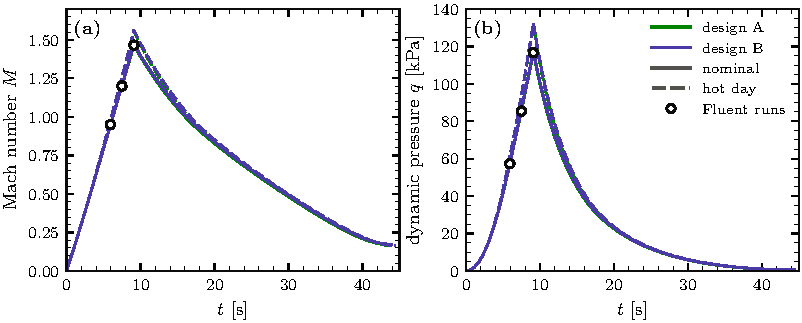
\includegraphics[width=0.9\linewidth]{fig_flight}
\caption{Mach number (a) and dynamic pressure (b) during the flight. Solid: nominal day; dashed: hot day.
The circles mark the three Fluent runs.}
\label{fig:flight}
\end{figure}

\subsection{Three load cases}

Three moments of the flight cover the largest air loads (Table~\ref{tab:lcs}).

\begin{table}[H]
\centering
\caption{The three load cases. Values for design A on a nominal day; design B differs by less than
0.5\,s. On a hot day burnout is reached at $M = \val{A-hot-LC1-M}$ and $q = \val{A-hot-LC1-q}$\,kPa.}
\label{tab:lcs}
\small
\begin{tabularx}{\linewidth}{@{}lcccc>{\raggedright\arraybackslash}X@{}}
\toprule
Load case & Time & Mach & Dynamic & Outside & Critical for\\
 & [s] & & pressure [kPa] & pressure [kPa] & \\
\midrule
\textbf{LC1, burnout} & \val{A-nominal-LC1-t} & \val{A-nominal-LC1-M} & \val{A-nominal-LC1-q} & \val{A-nominal-LC1-pinf} &
inward pressure on the tip, drag, side force and heating\\
\addlinespace
\textbf{LC2, transonic} & \val{A-nominal-LC2-t} & \val{A-nominal-LC2-M} & \val{A-nominal-LC2-q} & \val{A-nominal-LC2-pinf} &
the flow pattern changes near Mach~1; loads lower than at LC1\\
\addlinespace
\textbf{LC3, apogee} & \val{A-nominal-LC3-t} & \val{A-nominal-LC3-M} & \val{A-nominal-LC3-q} & \val{A-nominal-LC3-pinf} &
lowest outside pressure: outward pressure and pull-off force of the sealed nose\\
\bottomrule
\end{tabularx}
\end{table}

\subsection{The sealed nose}

The nose has no vent holes, so the air inside keeps the pressure it had on the pad,
$p_{pad} = \val{pad-p}$\,kPa. When the shell heats this air, its pressure rises:
\begin{equation}
p_{in} = p_{pad}\,\frac{T_{in}}{T_{pad}}.
\label{eq:dp}
\end{equation}
The temperature of the inside air $T_{in}$ is not computed. Two bounds are used instead:
\begin{itemize}
\item \textbf{cold inside air}, $T_{in} = T_{pad}$: lowest inside pressure, so the largest
\emph{inward} load;
\item \textbf{heated inside air}, $T_{in}$ = mean temperature of the inner face of the shell: highest
inside pressure, so the largest \emph{outward} load.
\end{itemize}
Each table says which bound it uses.

\subsection{Sign conventions}

Figure~\ref{fig:conventions} shows the conventions used everywhere in this report.
\begin{itemize}
\item $x$ is the distance from the tip along the axis. Four stations are followed during the flight:
the tip, 50\,mm, mid-length (half the curved part) and the shoulder (end of the curved part, where the
coupler starts).
\item The \textbf{net pressure} on the shell is $\Delta p = p_w - p_{in}$: the pressure on the outside of
the wall minus the pressure inside. $\Delta p > 0$ pushes the shell \textbf{inward}; $\Delta p < 0$ pushes
it \textbf{outward}.
\item An \textbf{axial force} $> 0$ is compression: it pushes the nose aft onto the joint. An axial
force $< 0$ is tension: it pulls the nose forward, off the joint.
\end{itemize}

\begin{figure}[H]
\centering
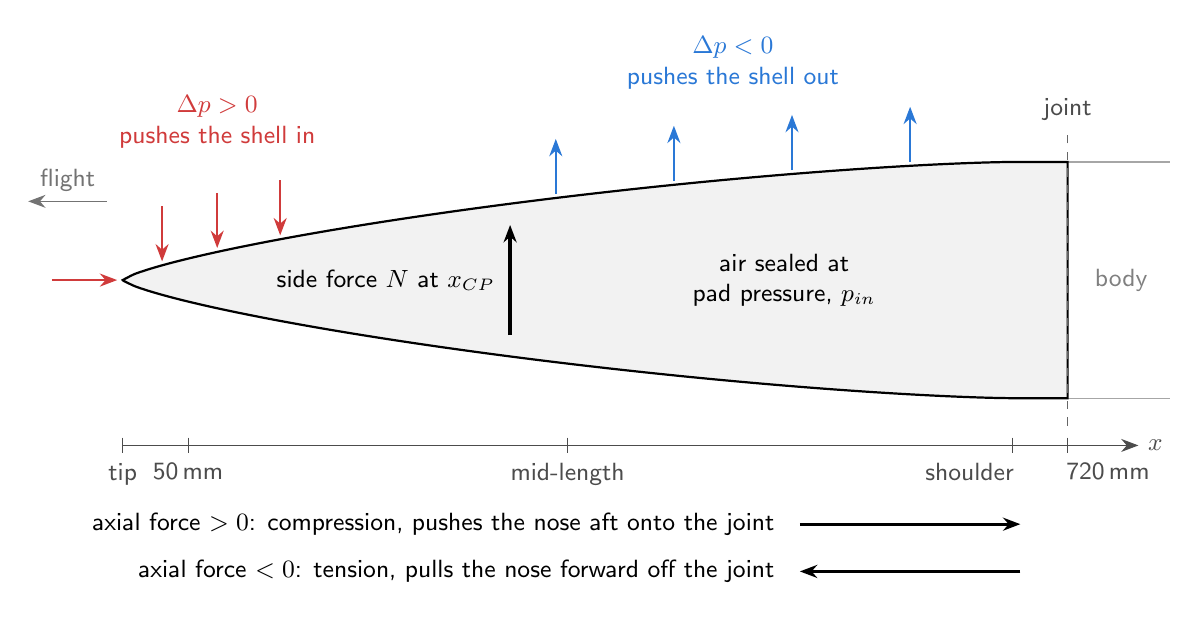
\begin{tikzpicture}[x=1cm, y=1cm, >={Stealth[length=2.2mm]},
  declare function={rr(\t) = 1.5*sqrt(max(0, (rad(acos(1 - 2*\t)) - 0.5*sin(2*acos(1 - 2*\t)))/pi));}]
  \def\xs{11.3}  % end of the curved part (60 mm per cm)
  \def\xj{12}    % joint plane, 720 mm
  % body tube behind the joint
  \draw[black!35] (\xj,1.5) -- (13.3,1.5) (\xj,-1.5) -- (13.3,-1.5);
  \node[black!50, font=\small] at (12.68,0) {body};
  % nose
  \filldraw[fill=black!5, draw=black, thick]
    plot[domain=0:1, samples=80, smooth] ({\xs*\x}, {rr(\x)}) -- (\xj,1.5) -- (\xj,-1.5)
    -- plot[domain=1:0, samples=80, smooth] ({\xs*\x}, {-rr(\x)}) -- cycle;
  % joint plane
  \draw[dashed, black!60] (\xj,-1.85) -- (\xj,1.9) node[above, font=\small, black!70] {joint};
  % inside air
  \node[font=\small, align=center] at (8.4,0) {air sealed at\\pad pressure, $p_{in}$};
  % flight direction
  \draw[->, black!55] (-0.2,1.0) -- (-1.2,1.0) node[midway, above, font=\small] {flight};
  % inward pressure on the front
  \foreach \px in {0.5, 1.2, 2.0}
    \draw[->, inward, thick] (\px, {rr(\px/\xs) + 0.75}) -- (\px, {rr(\px/\xs) + 0.05});
  \draw[->, inward, thick] (-0.9,0) -- (-0.07,0);
  \node[inward, font=\small, anchor=south, align=center] at (1.2,1.55) {$\Delta p > 0$\\pushes the shell in};
  % outward pressure on the rest of the shell
  \foreach \px in {5.5, 7.0, 8.5, 10.0}
    \draw[->, outward, thick] (\px, {rr(\px/\xs) + 0.05}) -- (\px, {rr(\px/\xs) + 0.75});
  \node[outward, font=\small, anchor=south, align=center] at (7.75,2.3) {$\Delta p < 0$\\pushes the shell out};
  % side force at the centre of pressure (design A)
  \draw[->, very thick] (4.92,-0.7) -- (4.92,0.7);
  \node[font=\small, anchor=east] at (4.85,0) {side force $N$ at $x_{CP}$};
  % stations
  \draw[->, black!70] (0,-2.1) -- (12.9,-2.1) node[right, font=\small] {$x$};
  \foreach \px/\lab in {0/tip, 0.83/50\,mm, 5.65/mid-length}
    \draw[black!70] (\px,-2.0) -- (\px,-2.2) node[below, font=\small] {\lab};
  \draw[black!70] (\xs,-2.0) -- (\xs,-2.2) node[anchor=north east, xshift=4pt, font=\small] {shoulder};
  \draw[black!70] (\xj,-2.0) -- (\xj,-2.2) node[anchor=north west, xshift=-4pt, font=\small] {720\,mm};
  % axial force convention
  \draw[->, very thick] (8.6,-3.1) -- (11.4,-3.1);
  \node[anchor=east, font=\small] at (8.4,-3.1) {axial force $> 0$: compression, pushes the nose aft onto the joint};
  \draw[->, very thick] (11.4,-3.7) -- (8.6,-3.7);
  \node[anchor=east, font=\small] at (8.4,-3.7) {axial force $< 0$: tension, pulls the nose forward off the joint};
\end{tikzpicture}
\caption{Sketch of the nose with the conventions used in all tables and figures.}
\label{fig:conventions}
\end{figure}

\section{Thermal profile}
\label{sec:heating}

\begin{keybox}
\begin{itemize}
\item At burnout the air stopped at the tip reaches the stagnation temperature,
\val{A-nominal-T0}--\val{B-nominal-T0}\,\si{\celsius} on a nominal day and
\val{A-hot-T0}--\val{B-hot-T0}\,\si{\celsius} on a hot day. Along the
rest of the nose the air drives the wall towards \val{A-Taw-far-lo}--\val{A-Taw-far-hi}\,K (about
107--110\,\si{\celsius}).
\item The shell is hottest just behind the tip and cools along the nose
(Figure~\ref{fig:thprofile}). The \textbf{outer face} stays below the \SI{120}{\celsius} of the DP490
bond everywhere: at most \val{th-B-nominal-Tout-hi}\,\si{\celsius} on a nominal day, but
\val{th-B-hot-Tout-hi}\,\si{\celsius} on a hot day, just behind the tip, a margin of only a few degrees.
\item The \textbf{inner face} goes above the \SI{67}{\celsius} of Req\_10 \textbf{over the whole length},
already on a nominal day: \val{th-A-nominal-Tin-lo} to \val{th-B-nominal-Tin-hi}\,\si{\celsius} (nominal)
and \val{th-A-hot-Tin-lo} to \val{th-B-hot-Tin-hi}\,\si{\celsius} (hot day). So does the air inside.
\item \textbf{A and B heat up the same way}: the shell temperatures differ by at most
\val{th-AB-diff}\,\si{\celsius}. Only the tip insert of B is 5--6\,\si{\celsius} cooler.
\end{itemize}
\end{keybox}

\subsection{What Fluent shows}

Burnout is the hottest moment of the flight: the rocket is at its highest speed, $M = \val{pt-M147-M}$.
Each design was run twice at this point:
\begin{itemize}
\item with an \textbf{adiabatic wall} (no heat goes into the wall): the wall then takes the temperature the
air drives it towards, the adiabatic wall temperature $T_{aw}$;
\item with the \textbf{wall held at \SI{300}{K}}: this gives the heat flux $q_w$ into a cold wall, and
from the two runs the heat-transfer coefficient $h = q_w/(T_{aw} - \SI{300}{K})$.
\end{itemize}

\paragraph{The air around the tip.} The air that hits the rounded tip is stopped and heats up to the
stagnation temperature. Figure~\ref{fig:tiptemp} follows this through the climb:
\begin{itemize}
\item at $M = 0.95$ there is no shock yet: the air warms up gradually as it approaches the tip, to
about 333\,K;
\item at $M = 1.20$ a bow shock stands ahead of the tip, and the air behind it reaches about 359\,K;
\item at burnout the shock sits closer to the tip and the air reaches about \SI{391}{K}, the hottest
moment of the flight.
\end{itemize}
The two tips look the same at every point: the tip radius is the same, and so is the heating. Further
back, the hot air stays in a thin layer along the wall, the boundary layer (Figure~\ref{fig:tempfield}).

\begin{figure}[H]
\centering
\begin{subfigure}[t]{0.325\linewidth}
\centering
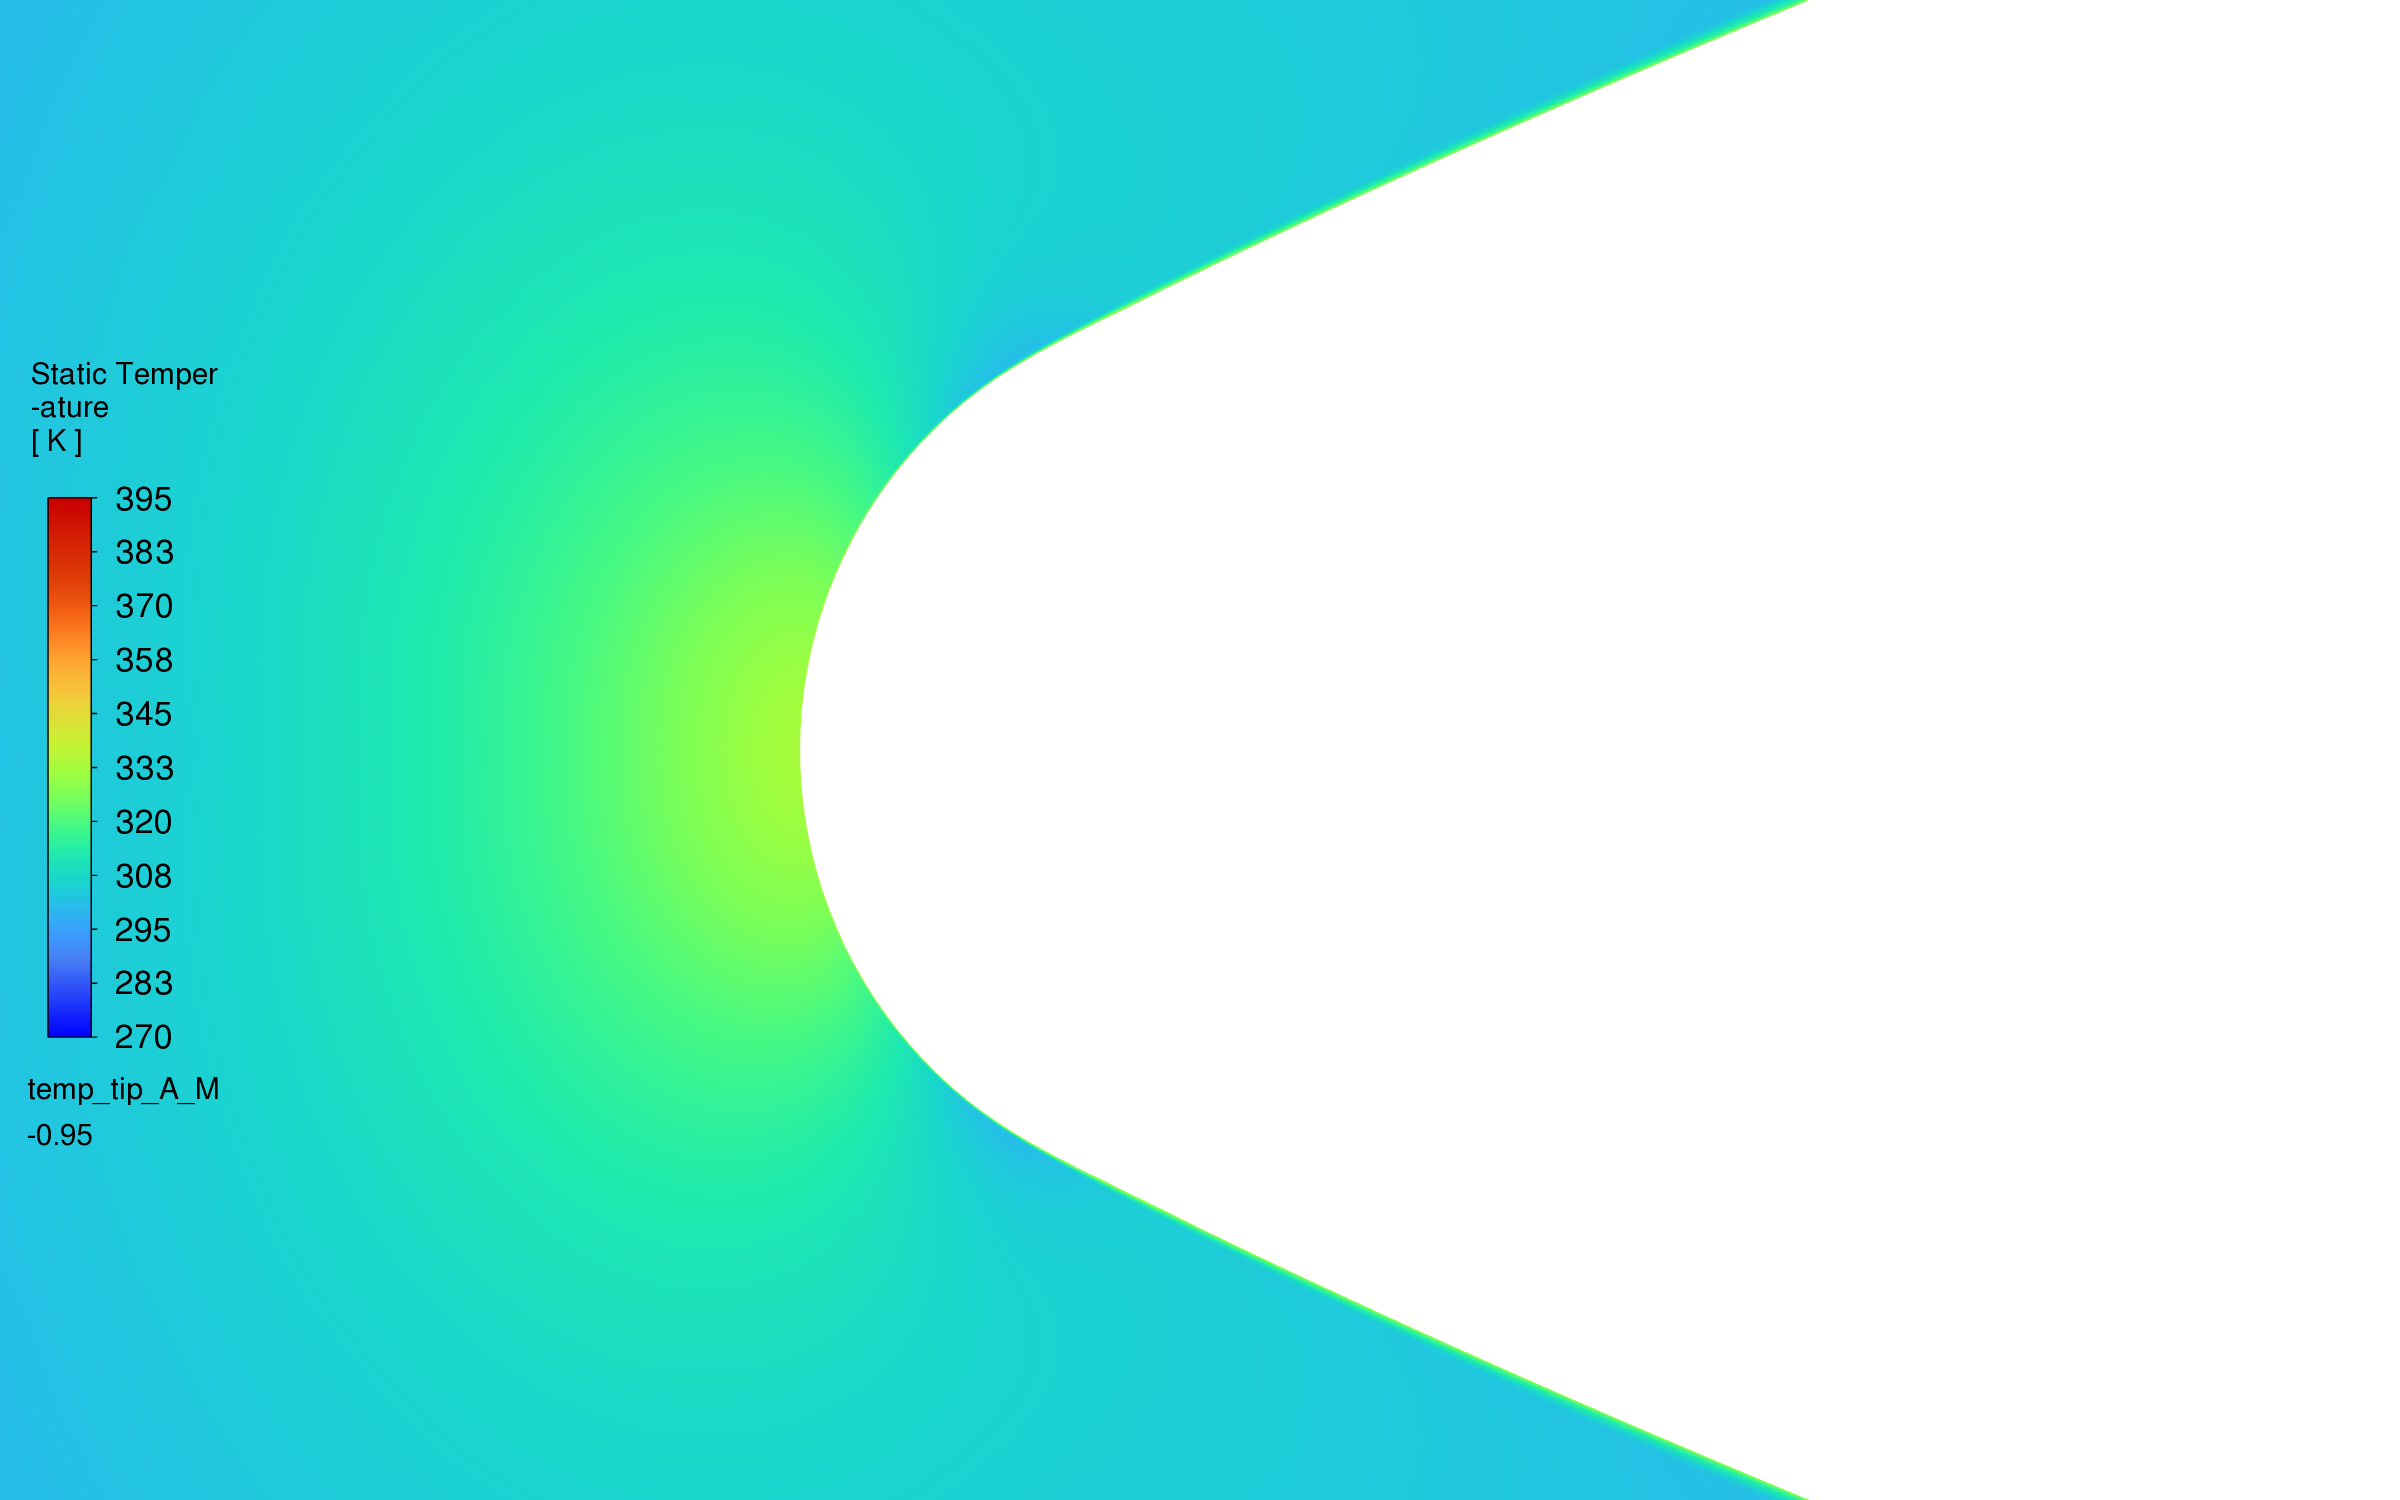
\includegraphics[width=\linewidth]{fluent_temp_tip_A_M0.95}
\caption{A, $M = 0.95$.}
\end{subfigure}\hfill
\begin{subfigure}[t]{0.325\linewidth}
\centering
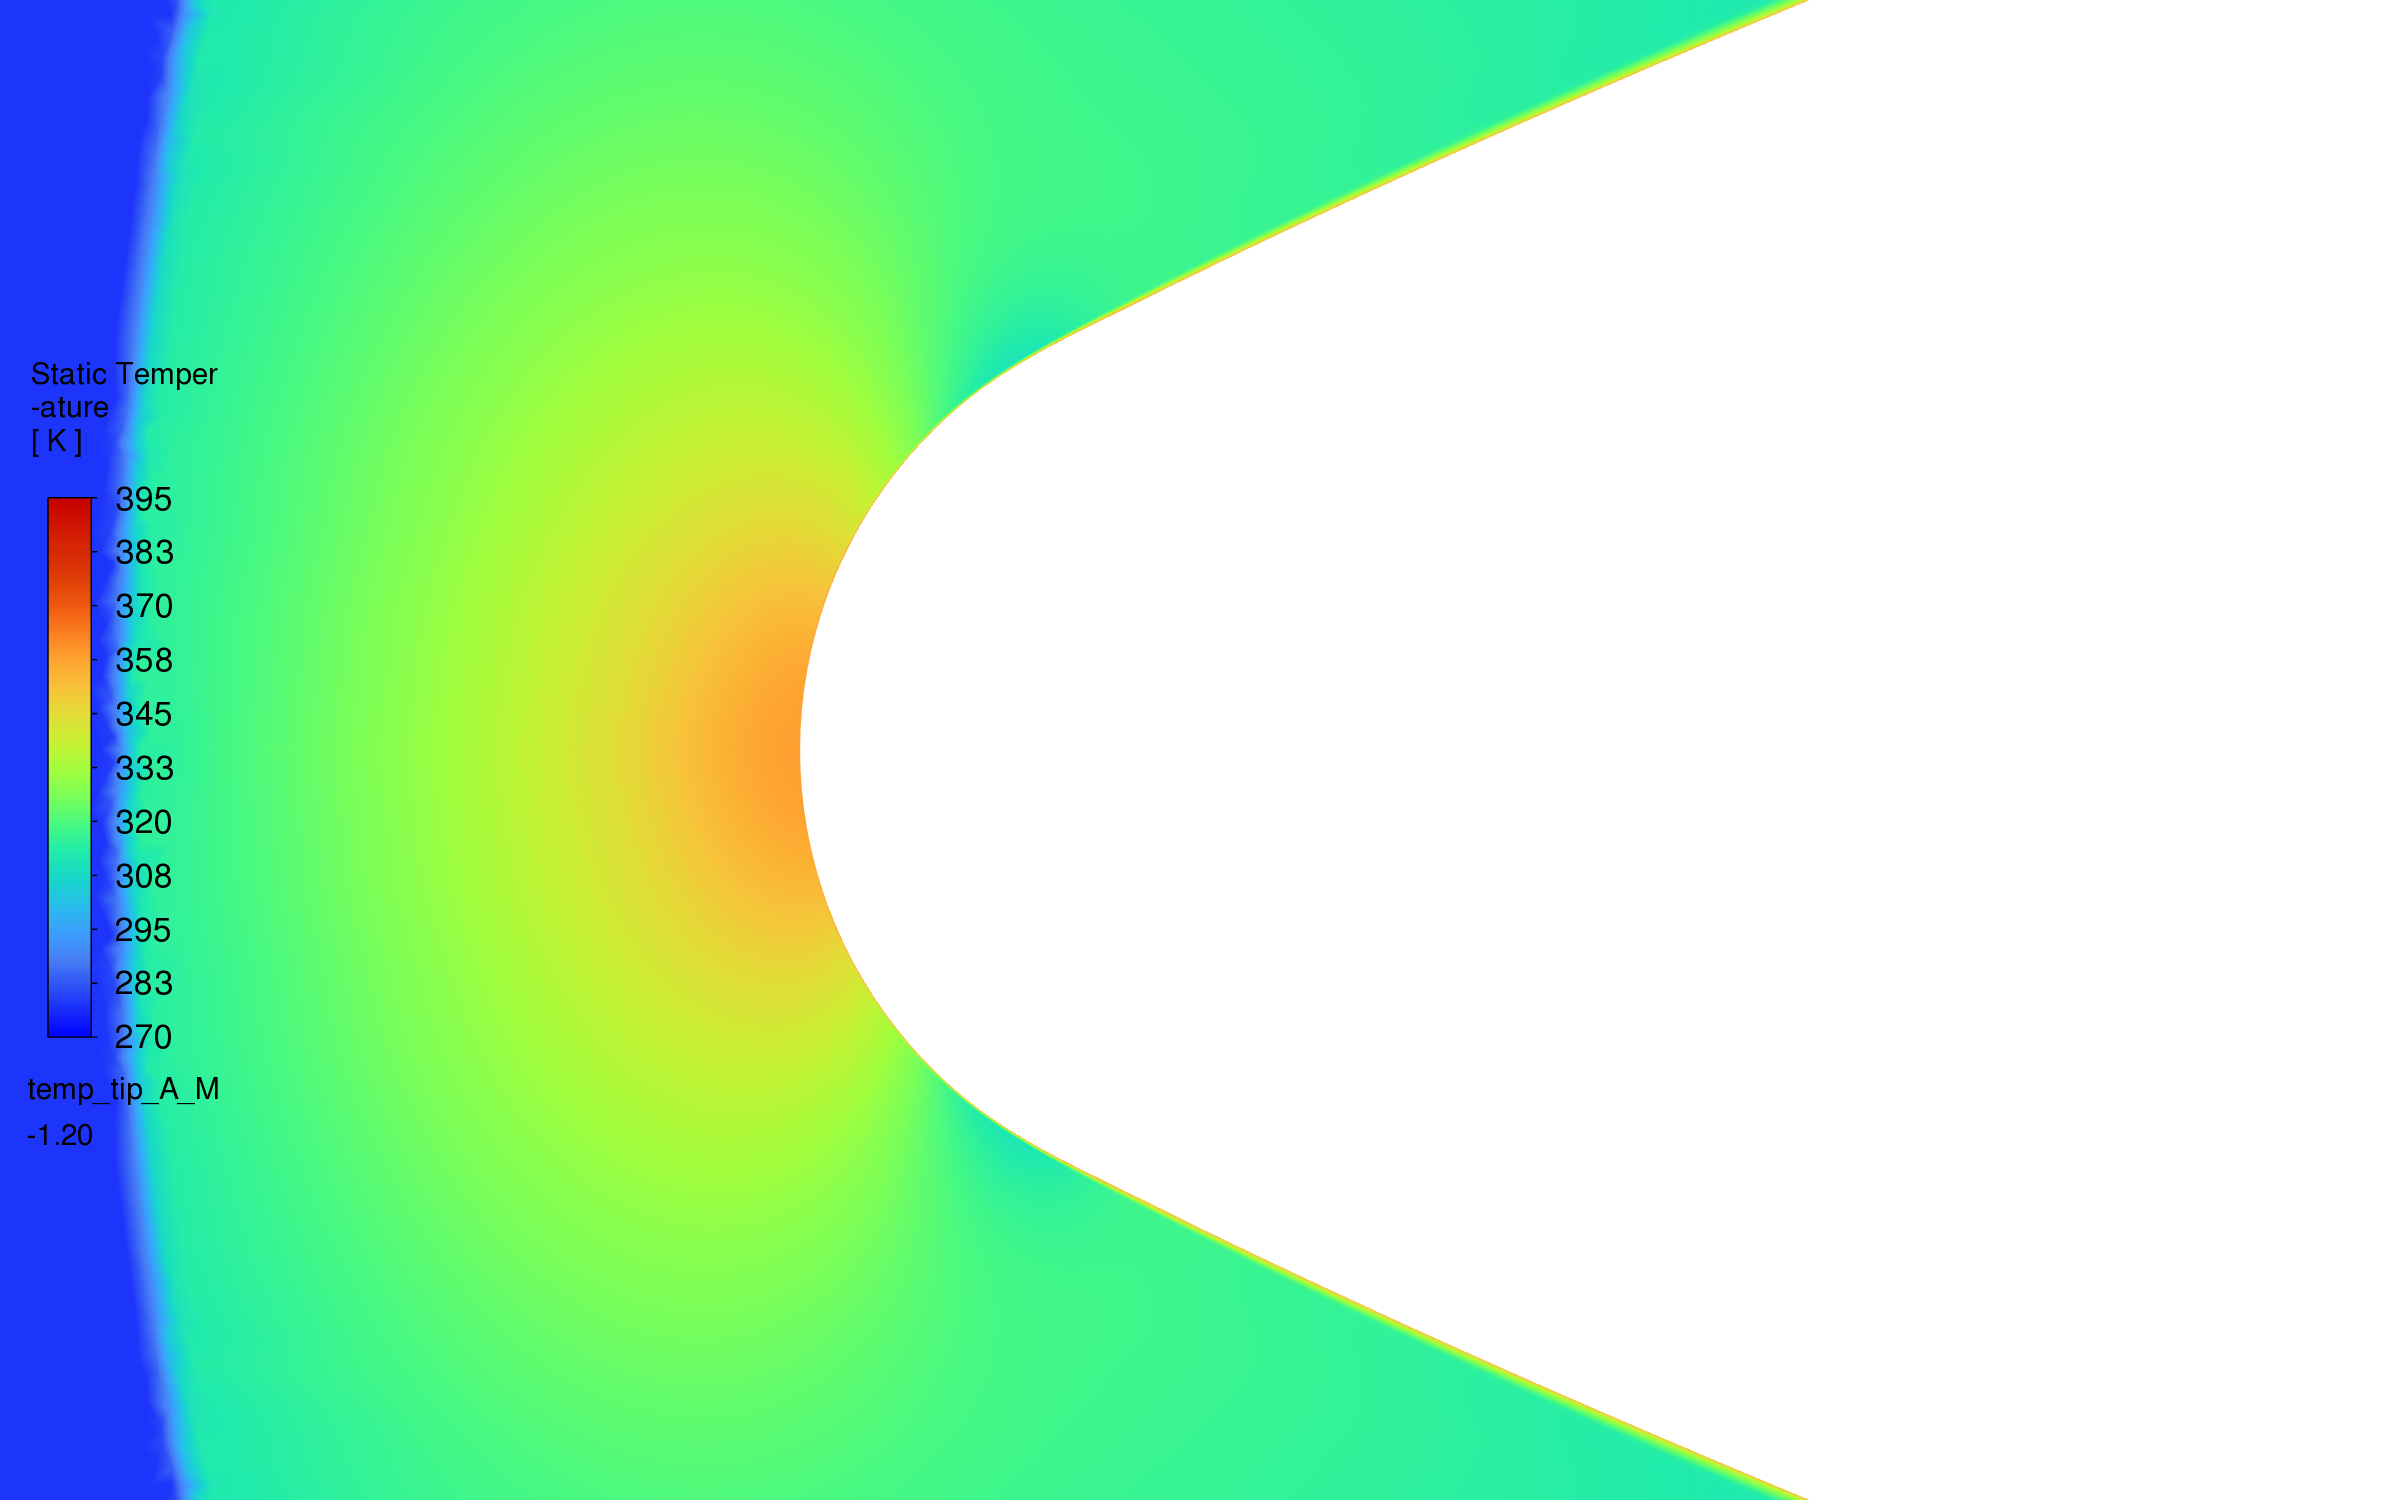
\includegraphics[width=\linewidth]{fluent_temp_tip_A_M1.20}
\caption{A, $M = 1.20$.}
\end{subfigure}\hfill
\begin{subfigure}[t]{0.325\linewidth}
\centering
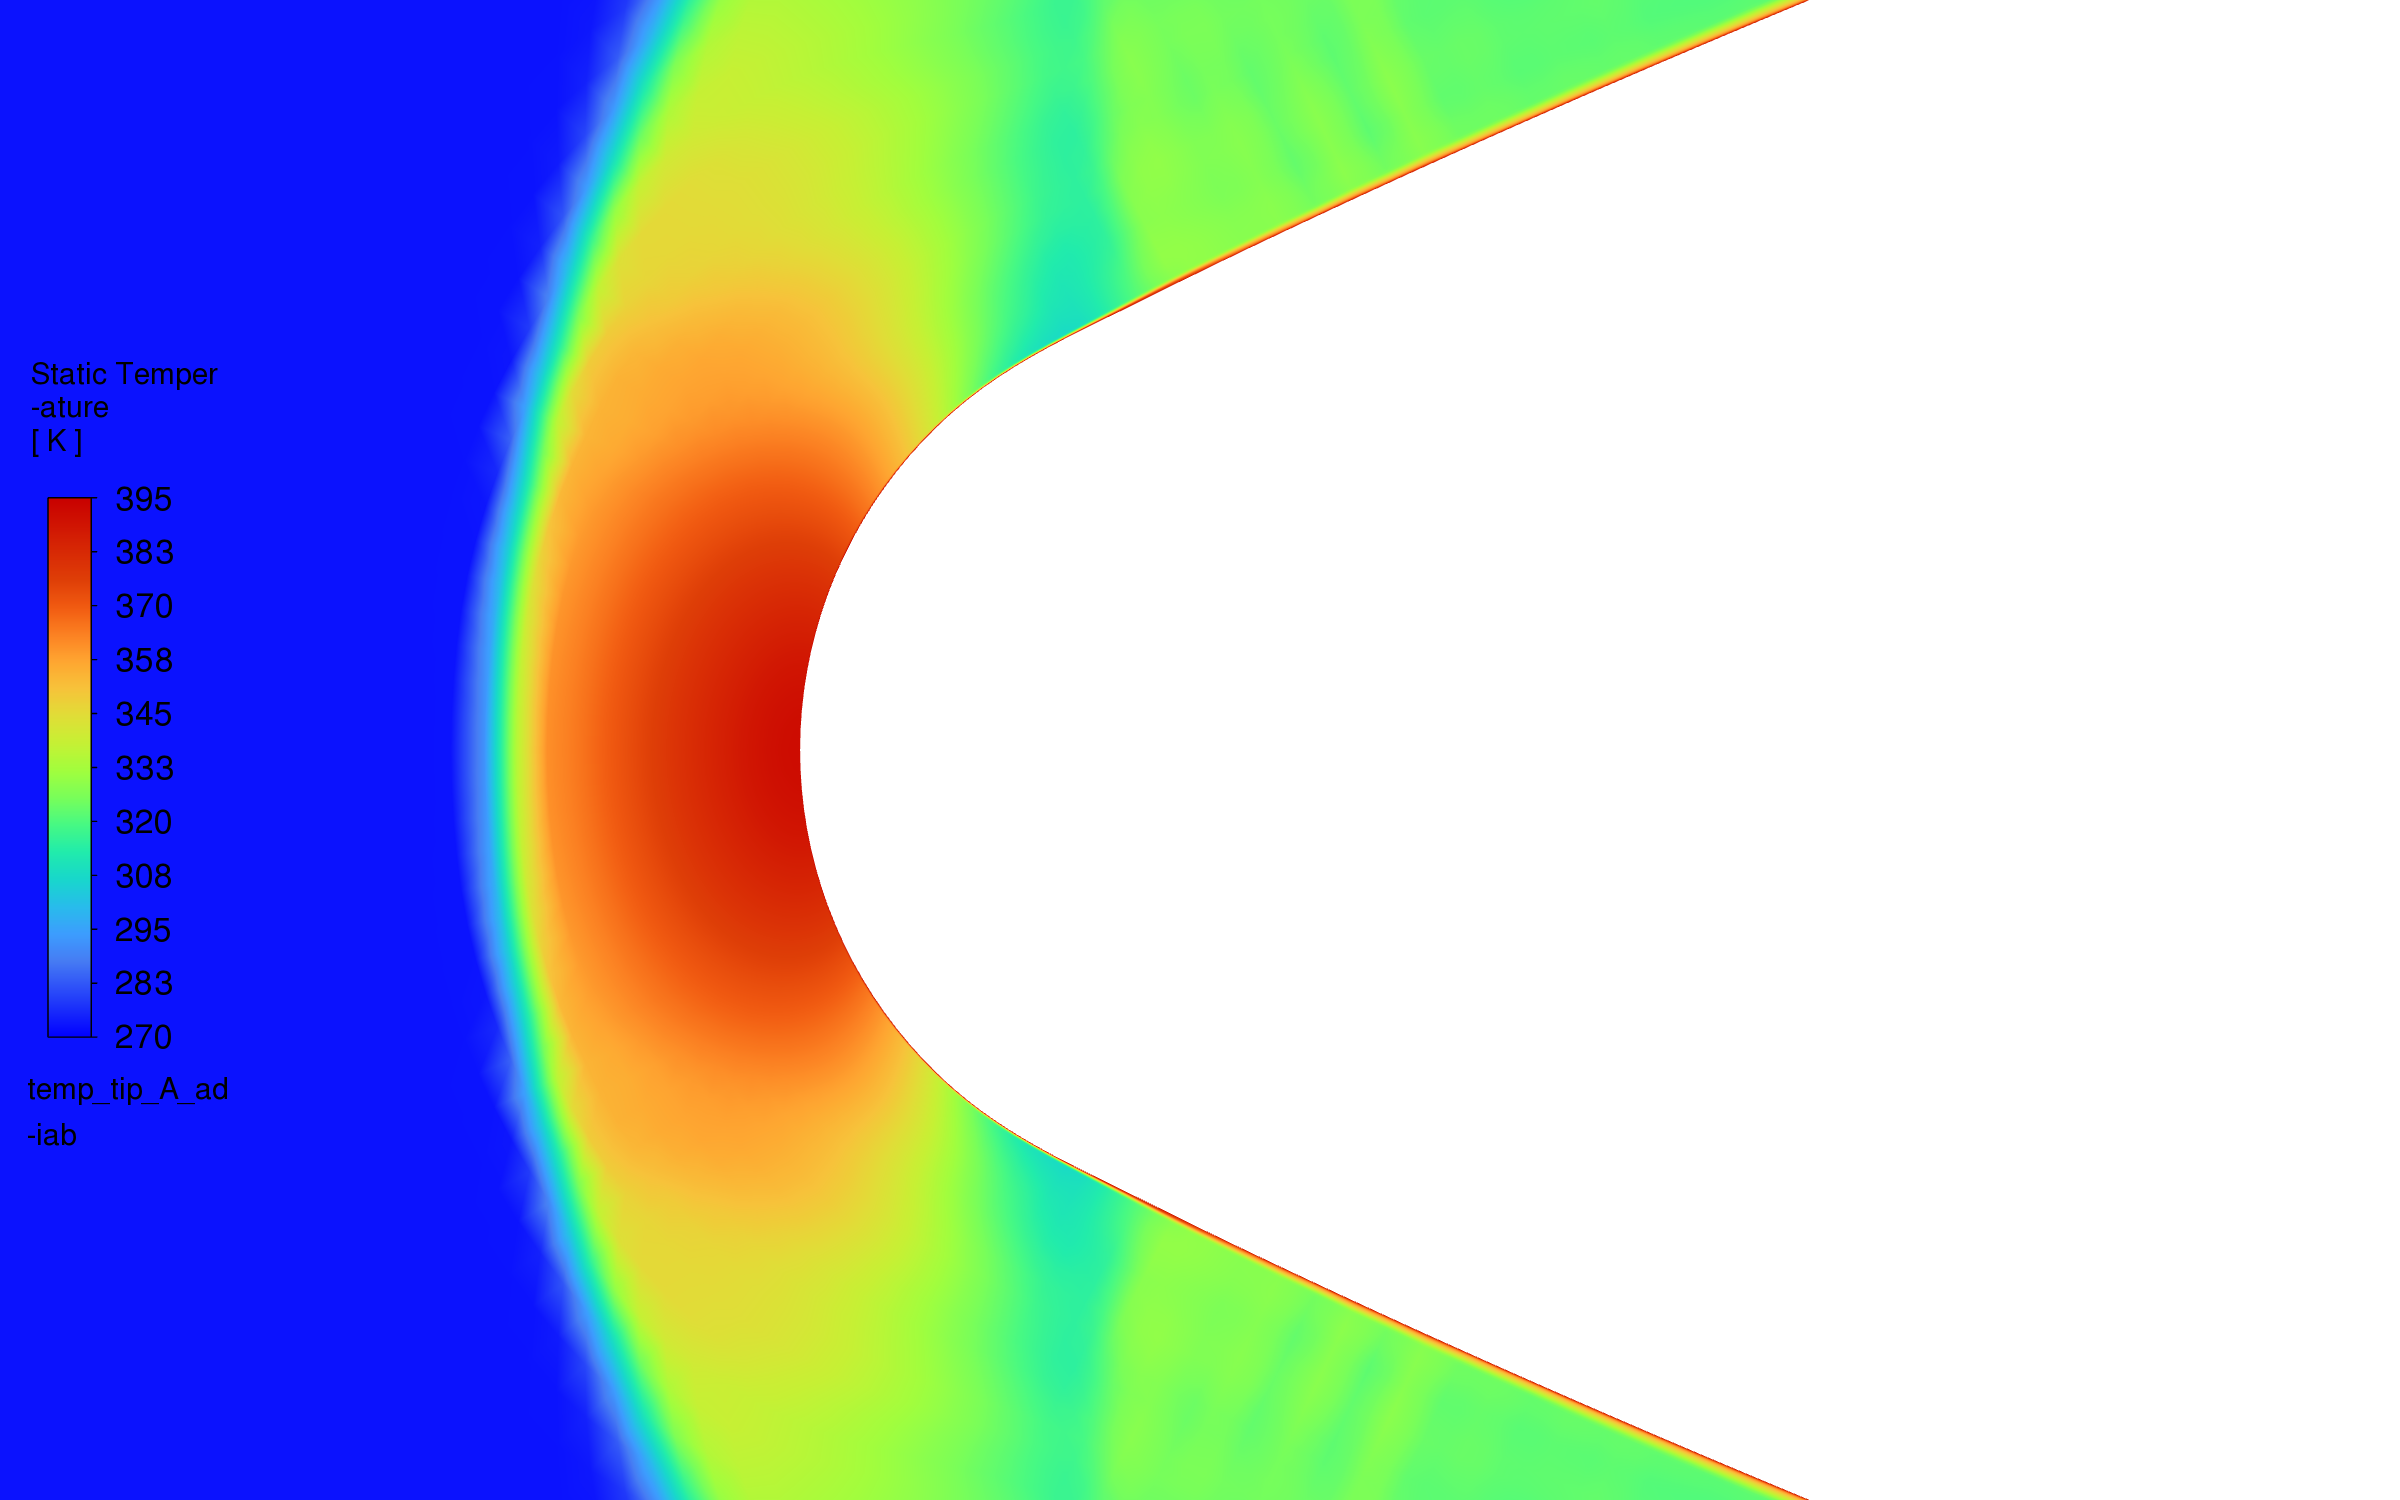
\includegraphics[width=\linewidth]{fluent_temp_tip_A_adiab}
\caption{A, burnout.}
\end{subfigure}

\smallskip
\begin{subfigure}[t]{0.325\linewidth}
\centering
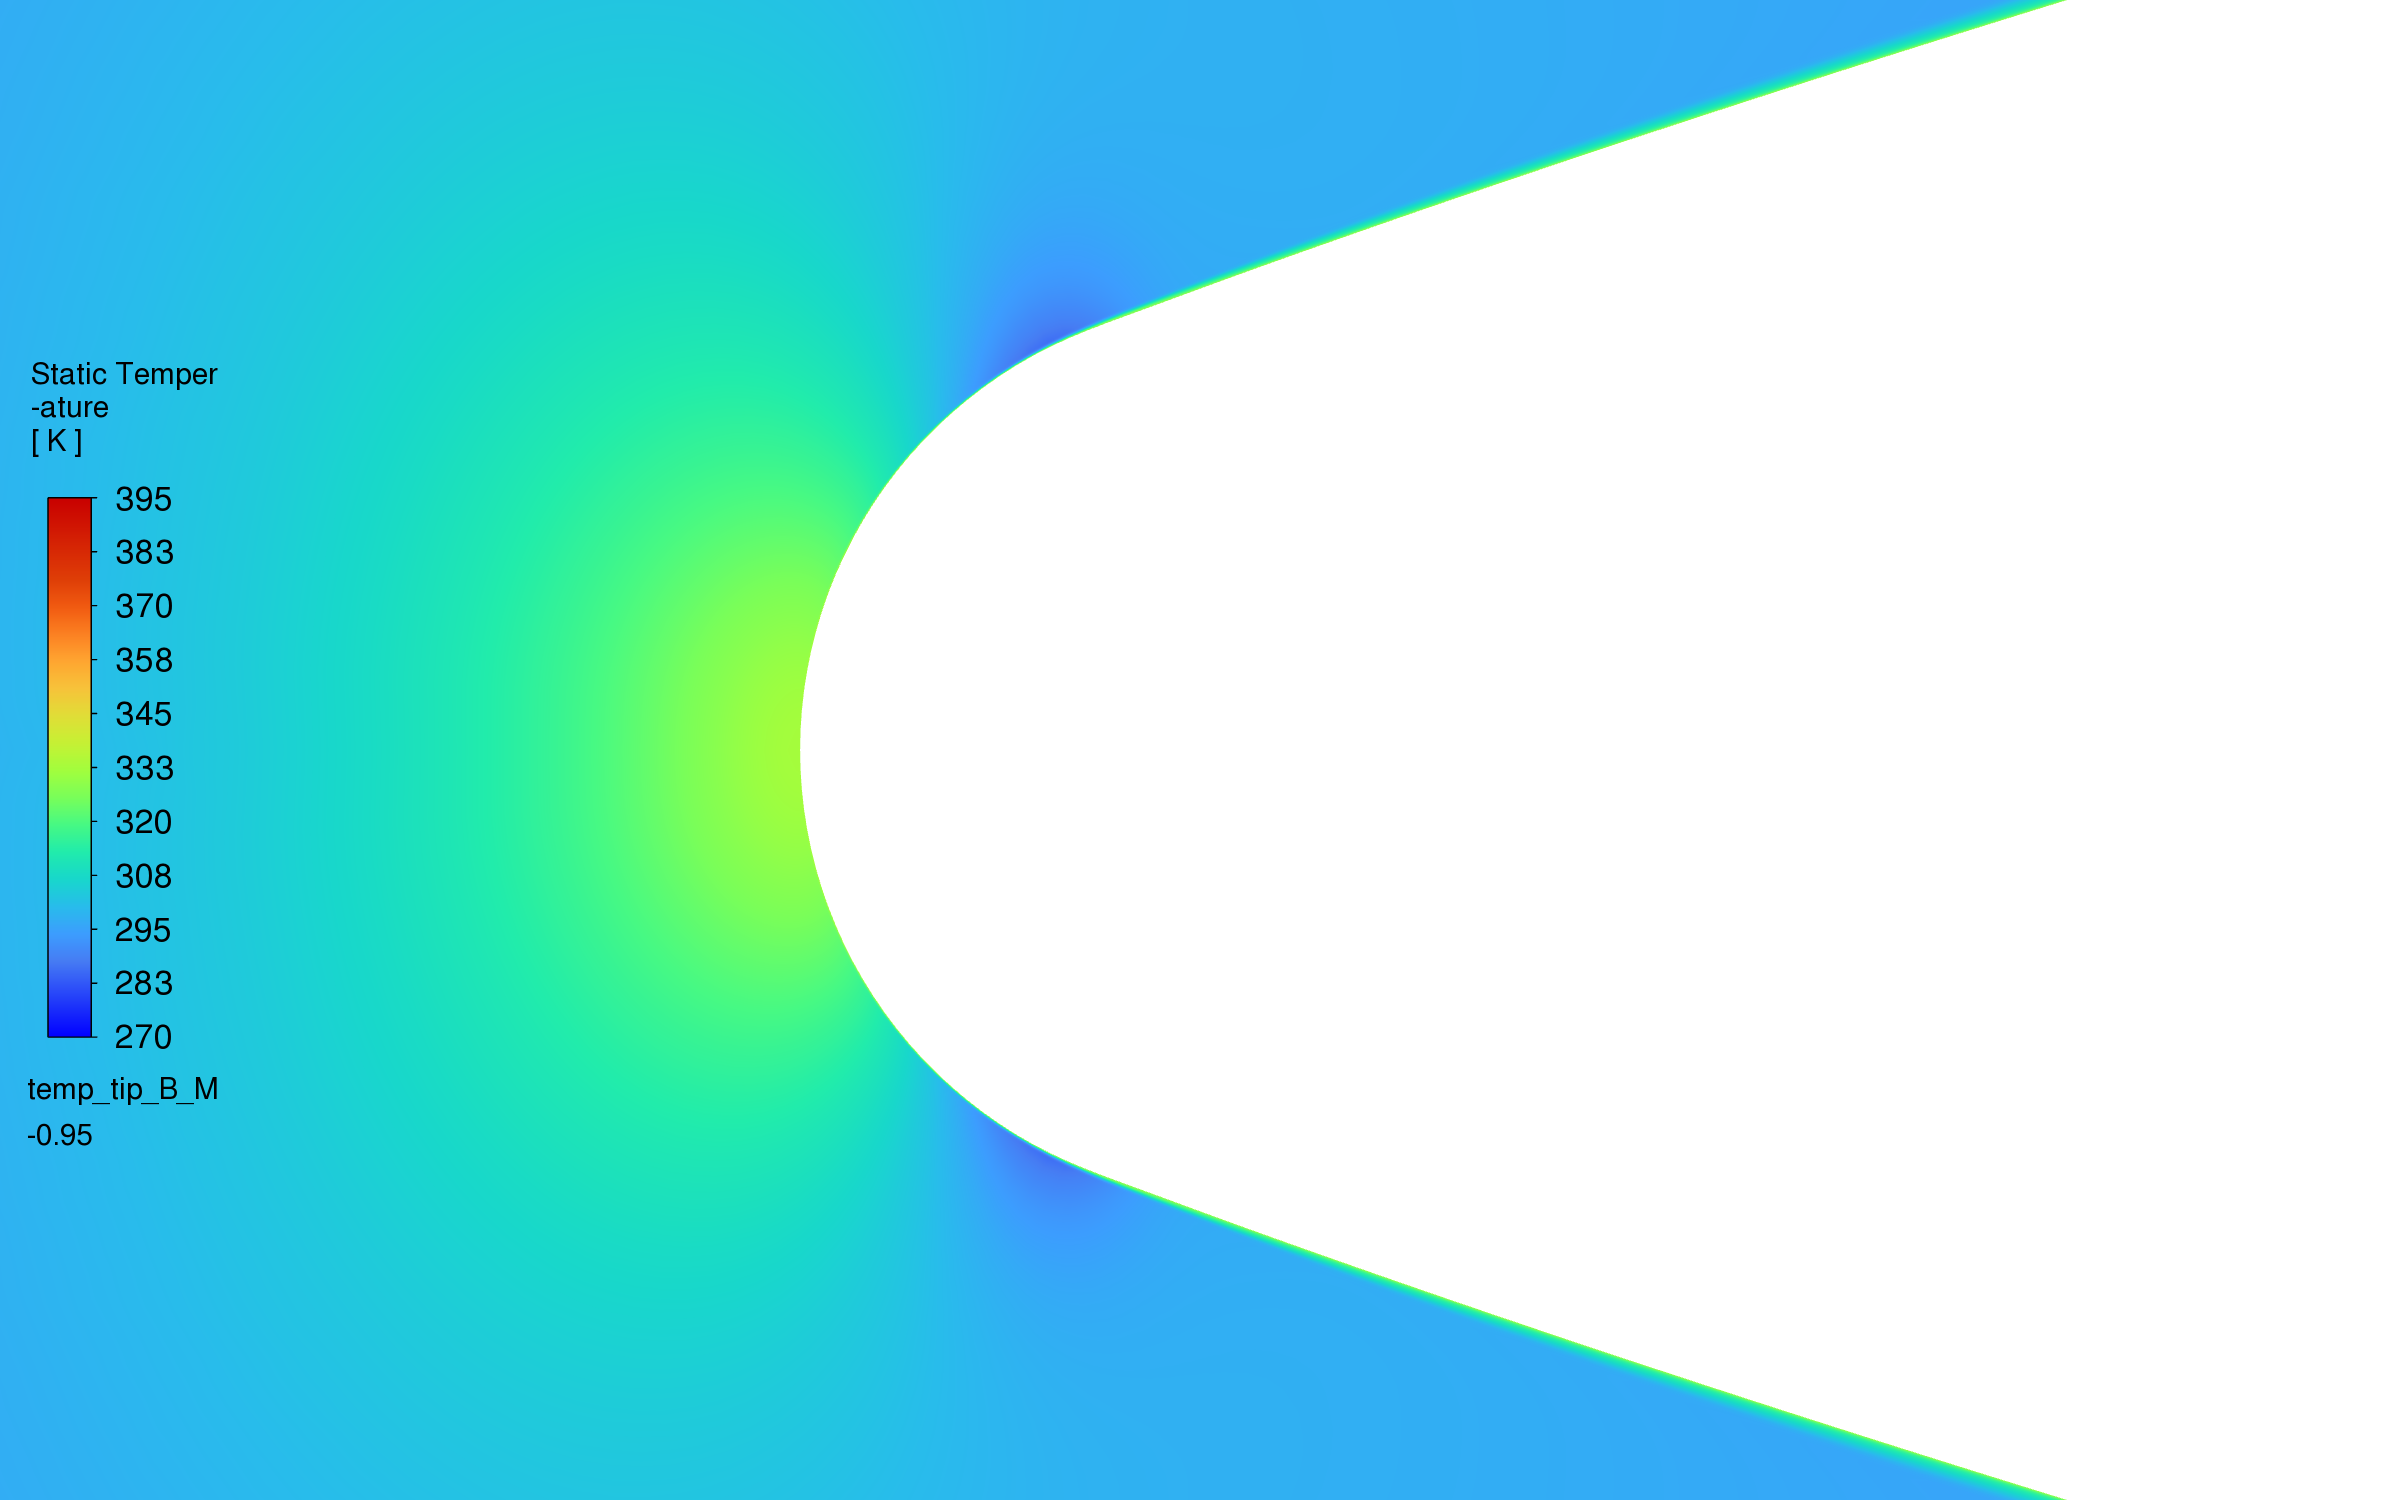
\includegraphics[width=\linewidth]{fluent_temp_tip_B_M0.95}
\caption{B, $M = 0.95$.}
\end{subfigure}\hfill
\begin{subfigure}[t]{0.325\linewidth}
\centering
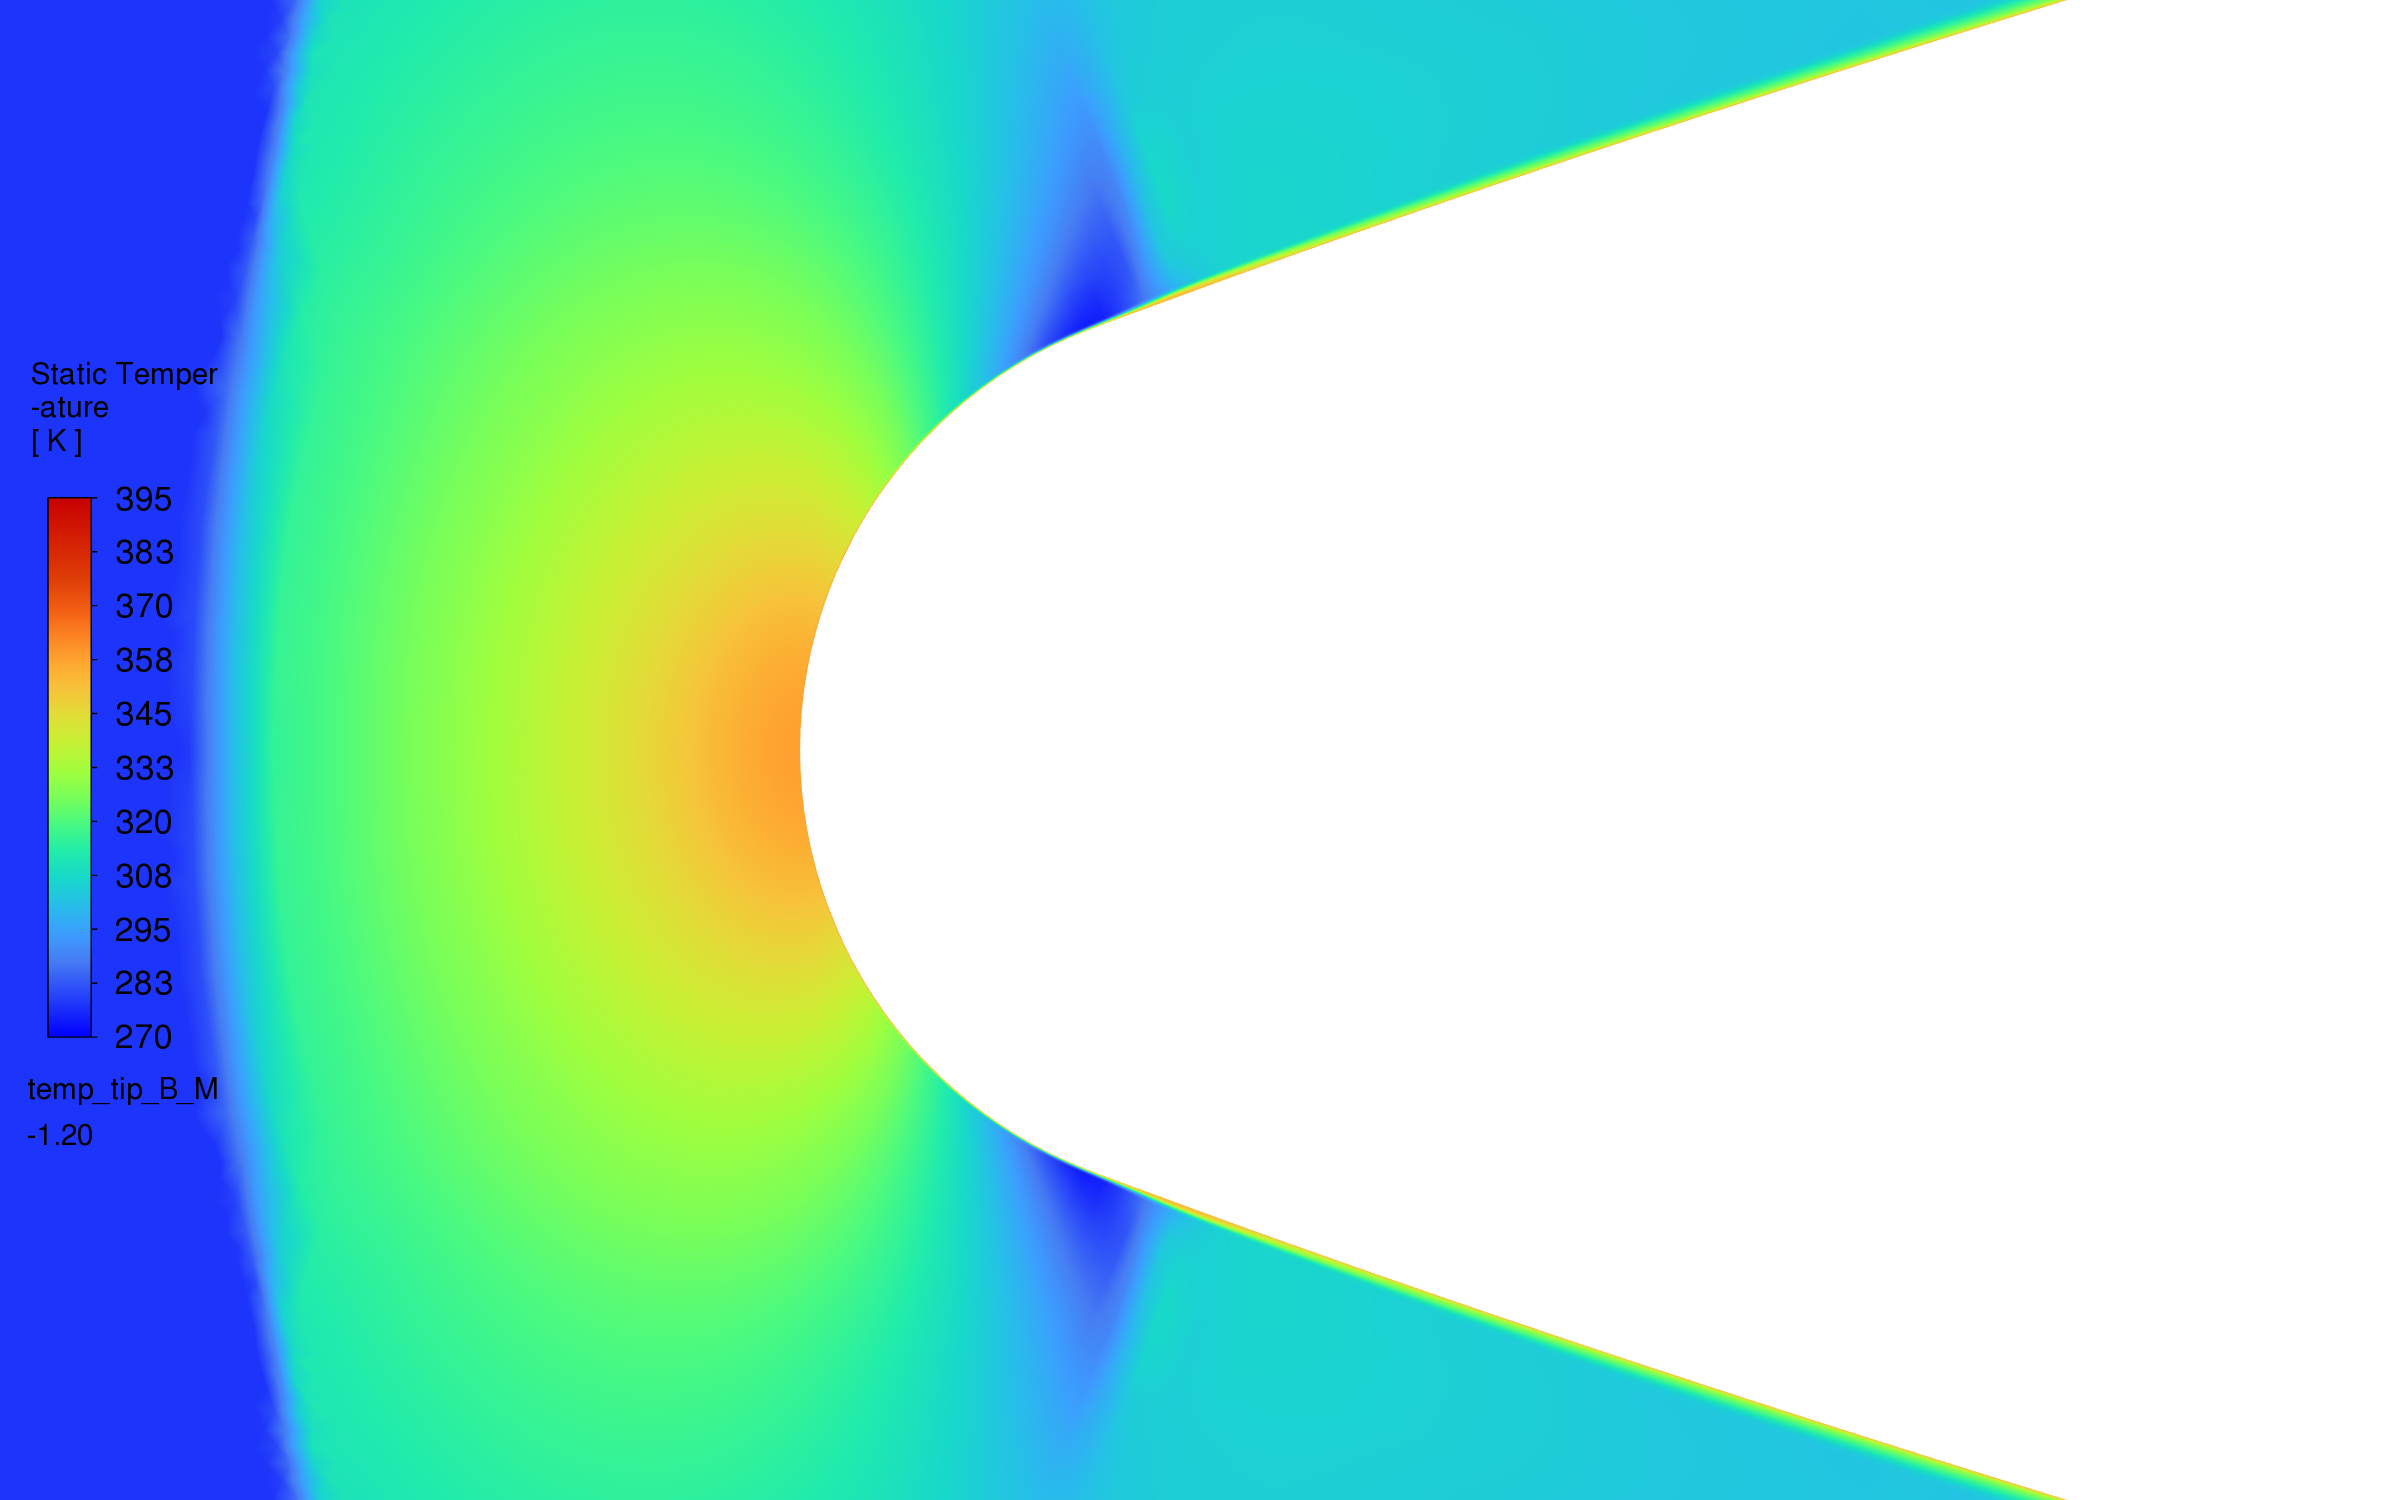
\includegraphics[width=\linewidth]{fluent_temp_tip_B_M1.20}
\caption{B, $M = 1.20$.}
\end{subfigure}\hfill
\begin{subfigure}[t]{0.325\linewidth}
\centering
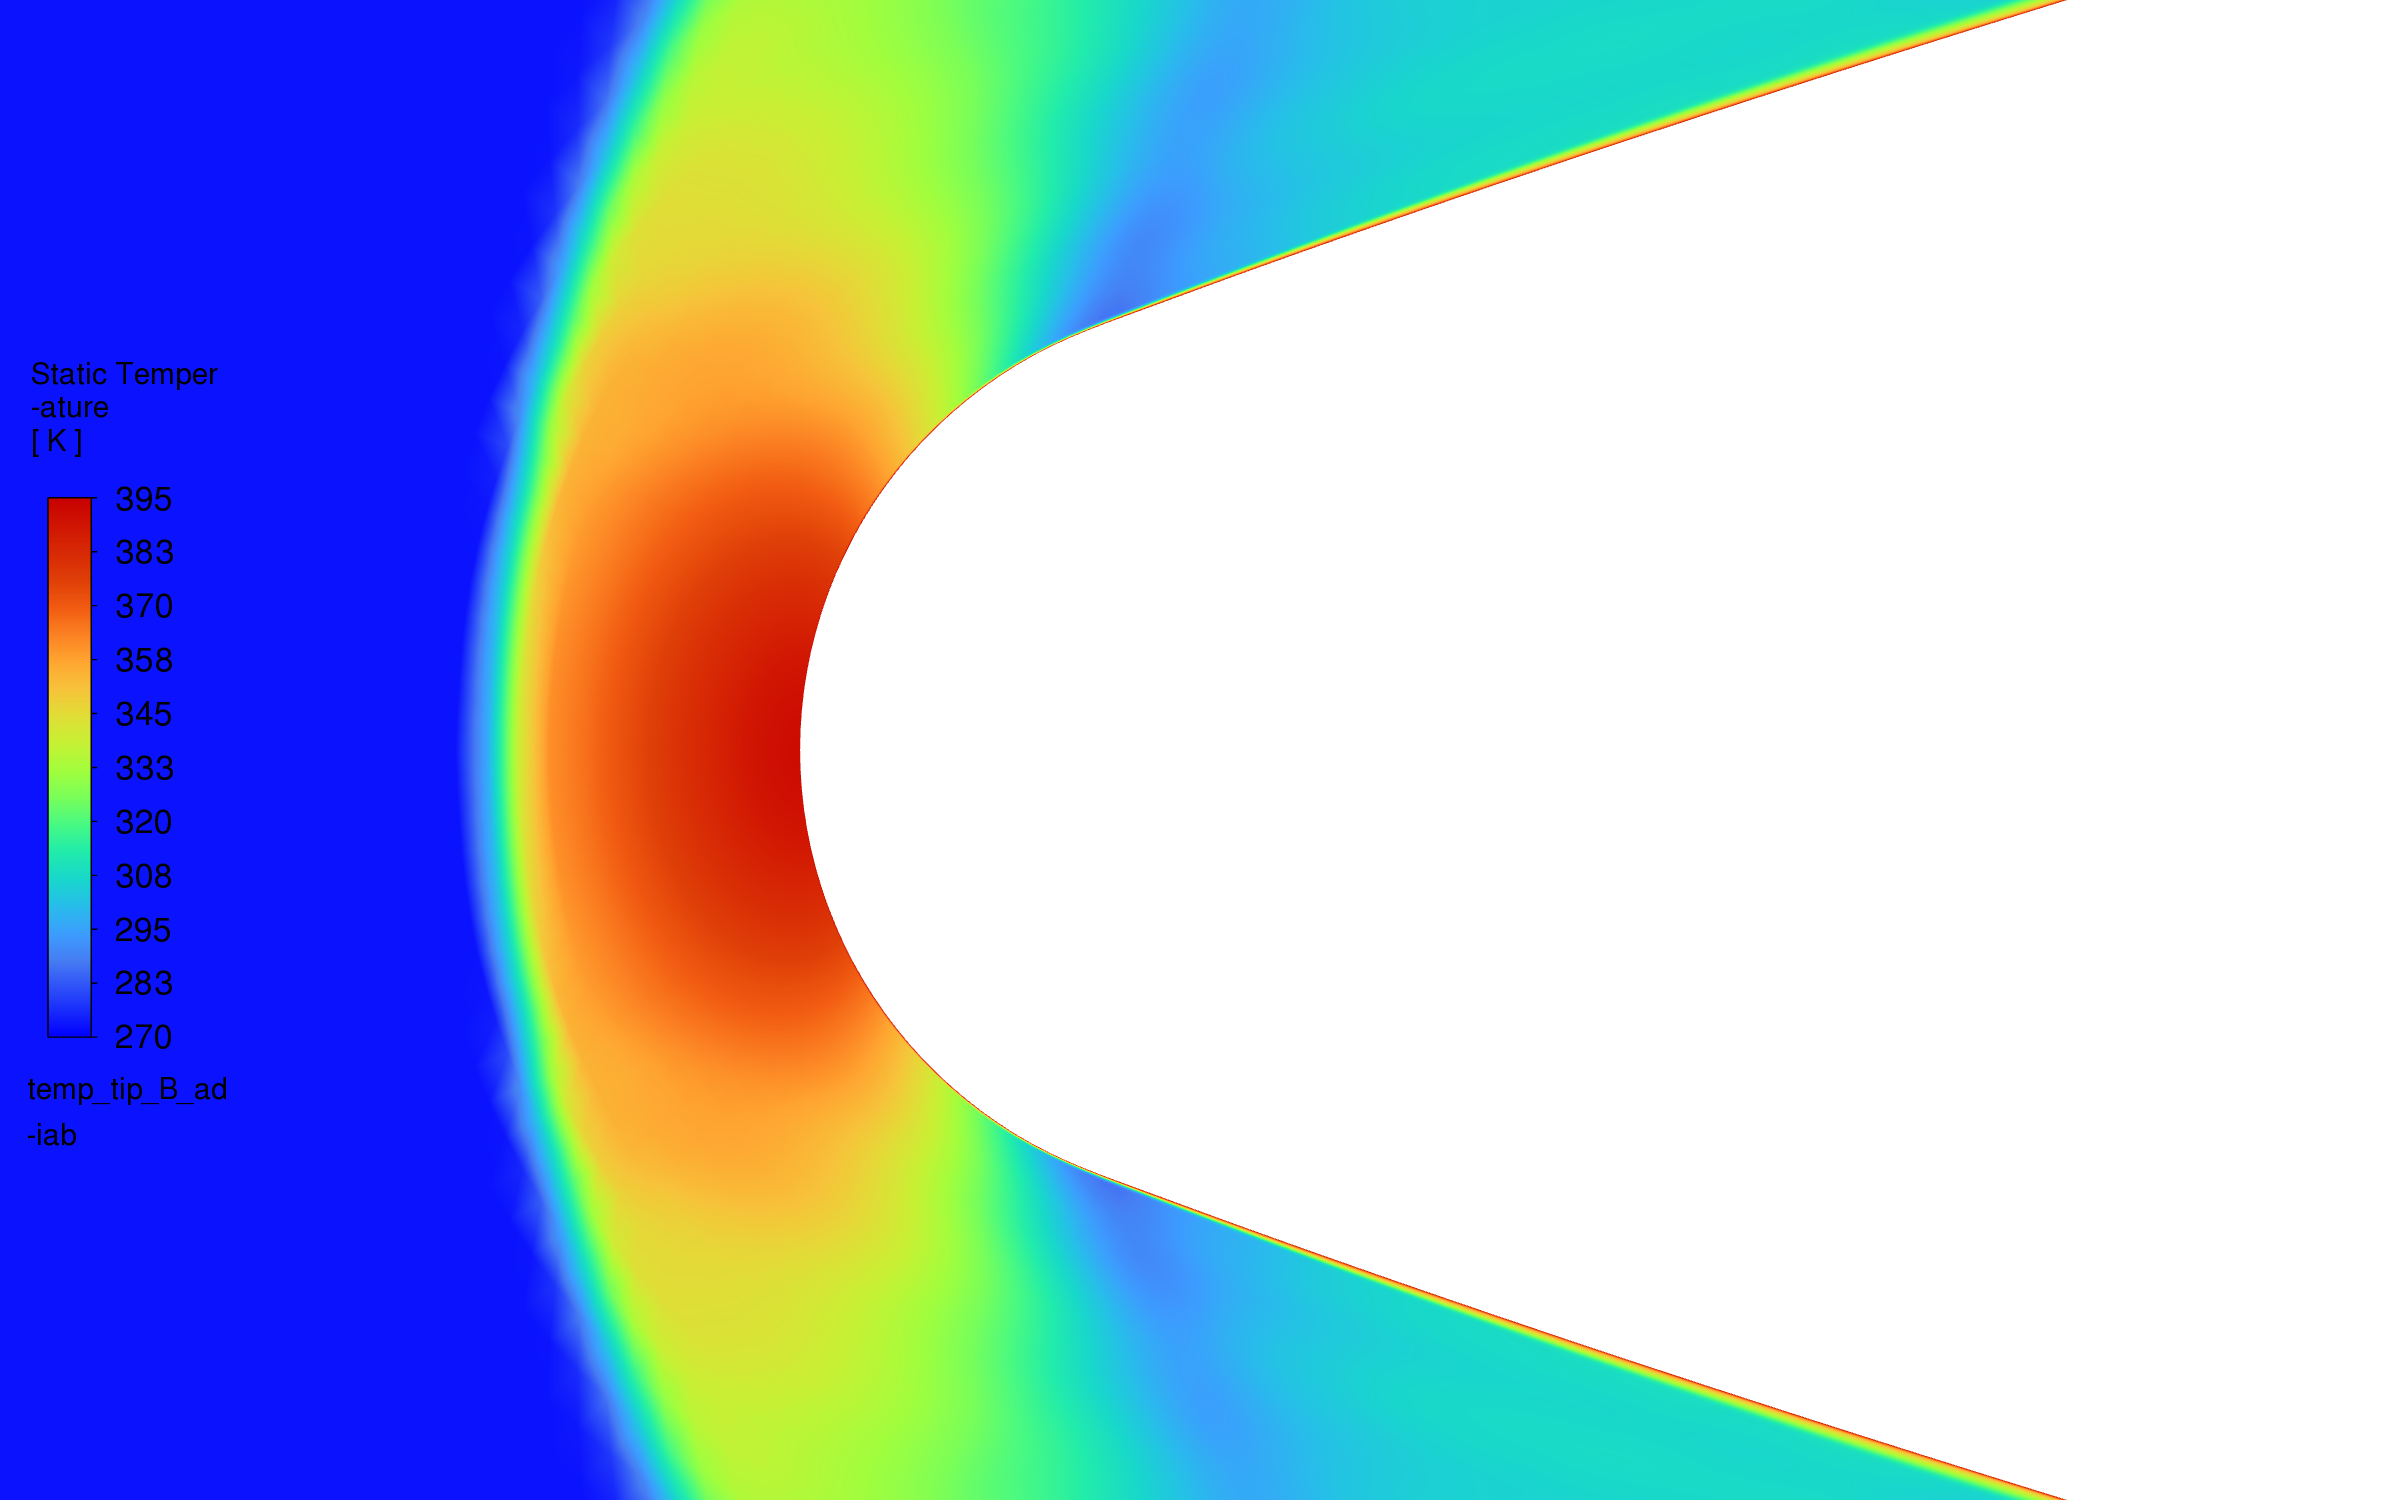
\includegraphics[width=\linewidth]{fluent_temp_tip_B_adiab}
\caption{B, burnout.}
\end{subfigure}
\caption{Air temperature around the tip at the three Fluent points of the climb (left to right: $M = 0.95$,
1.20 and burnout, $M = \val{pt-M147-M}$), adiabatic wall; top: design A, bottom: design B. Same colour
scale in all: 270\,K (blue) to 395\,K (red). The air at the tip heats up from about 333\,K to 359\,K and
391\,K.}
\label{fig:tiptemp}
\end{figure}

\begin{figure}[H]
\centering
\begin{subfigure}[t]{0.49\linewidth}
\centering
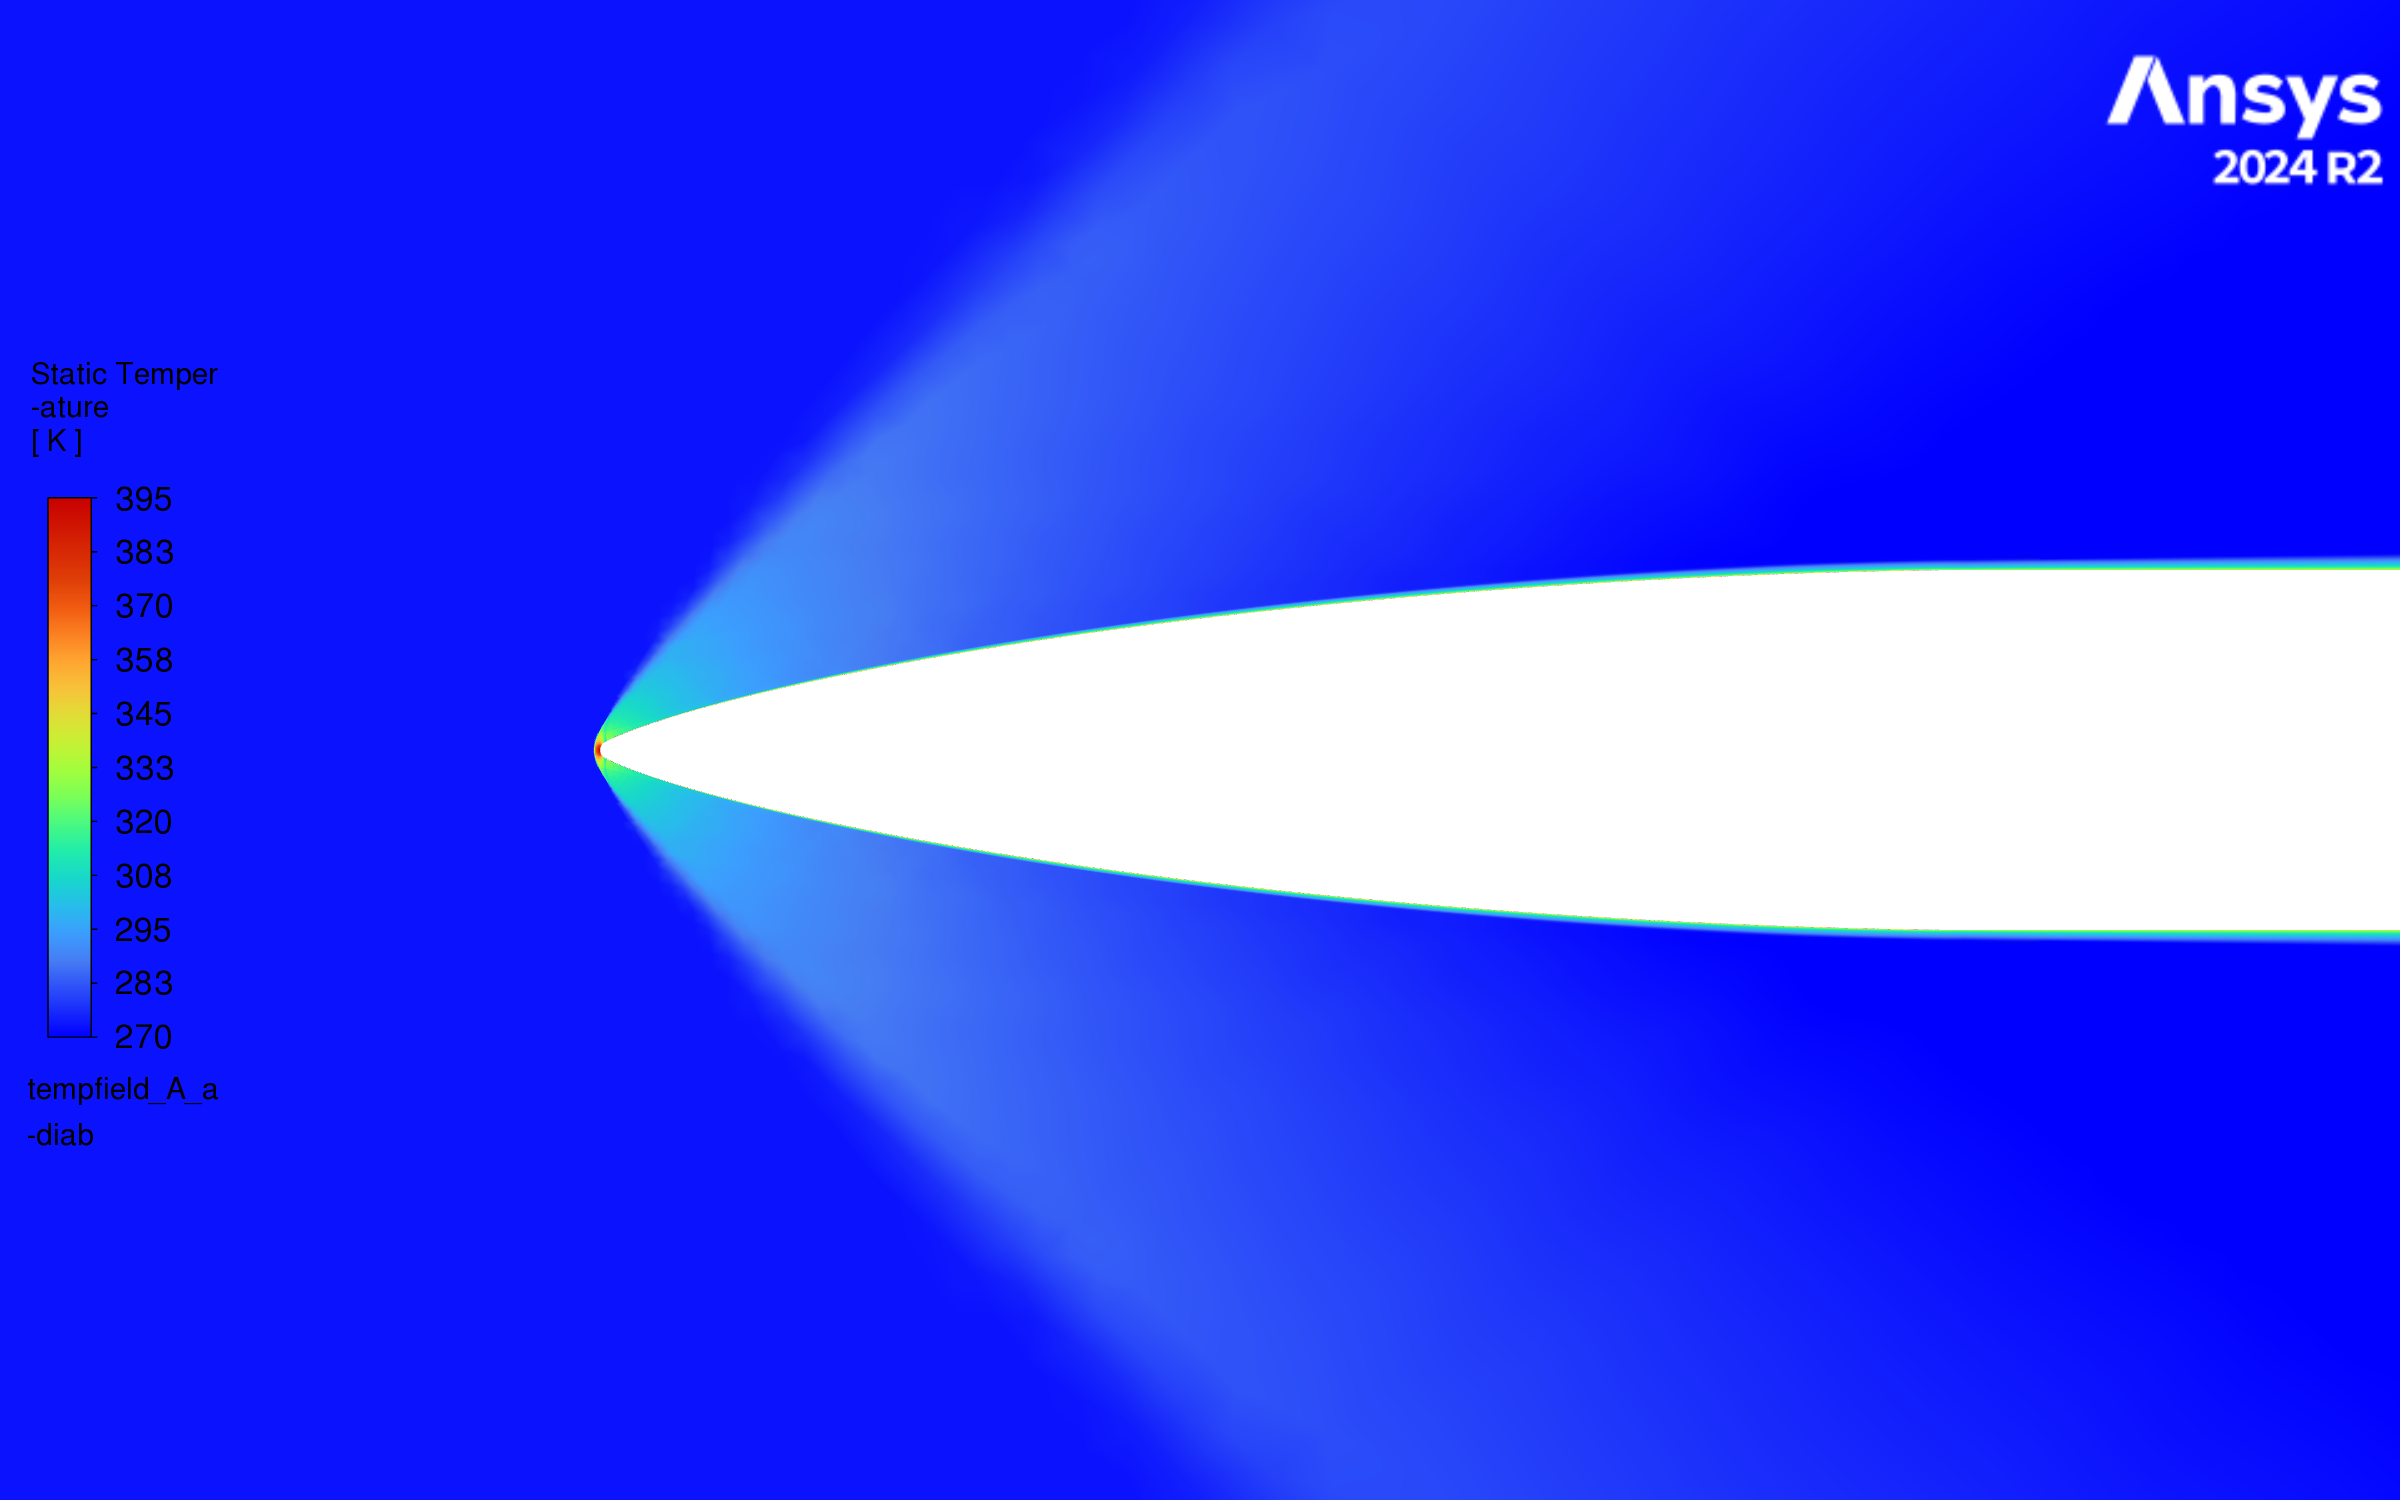
\includegraphics[width=\linewidth]{fluent_tempfield_A_adiab}
\caption{Design A.}
\end{subfigure}\hfill
\begin{subfigure}[t]{0.49\linewidth}
\centering
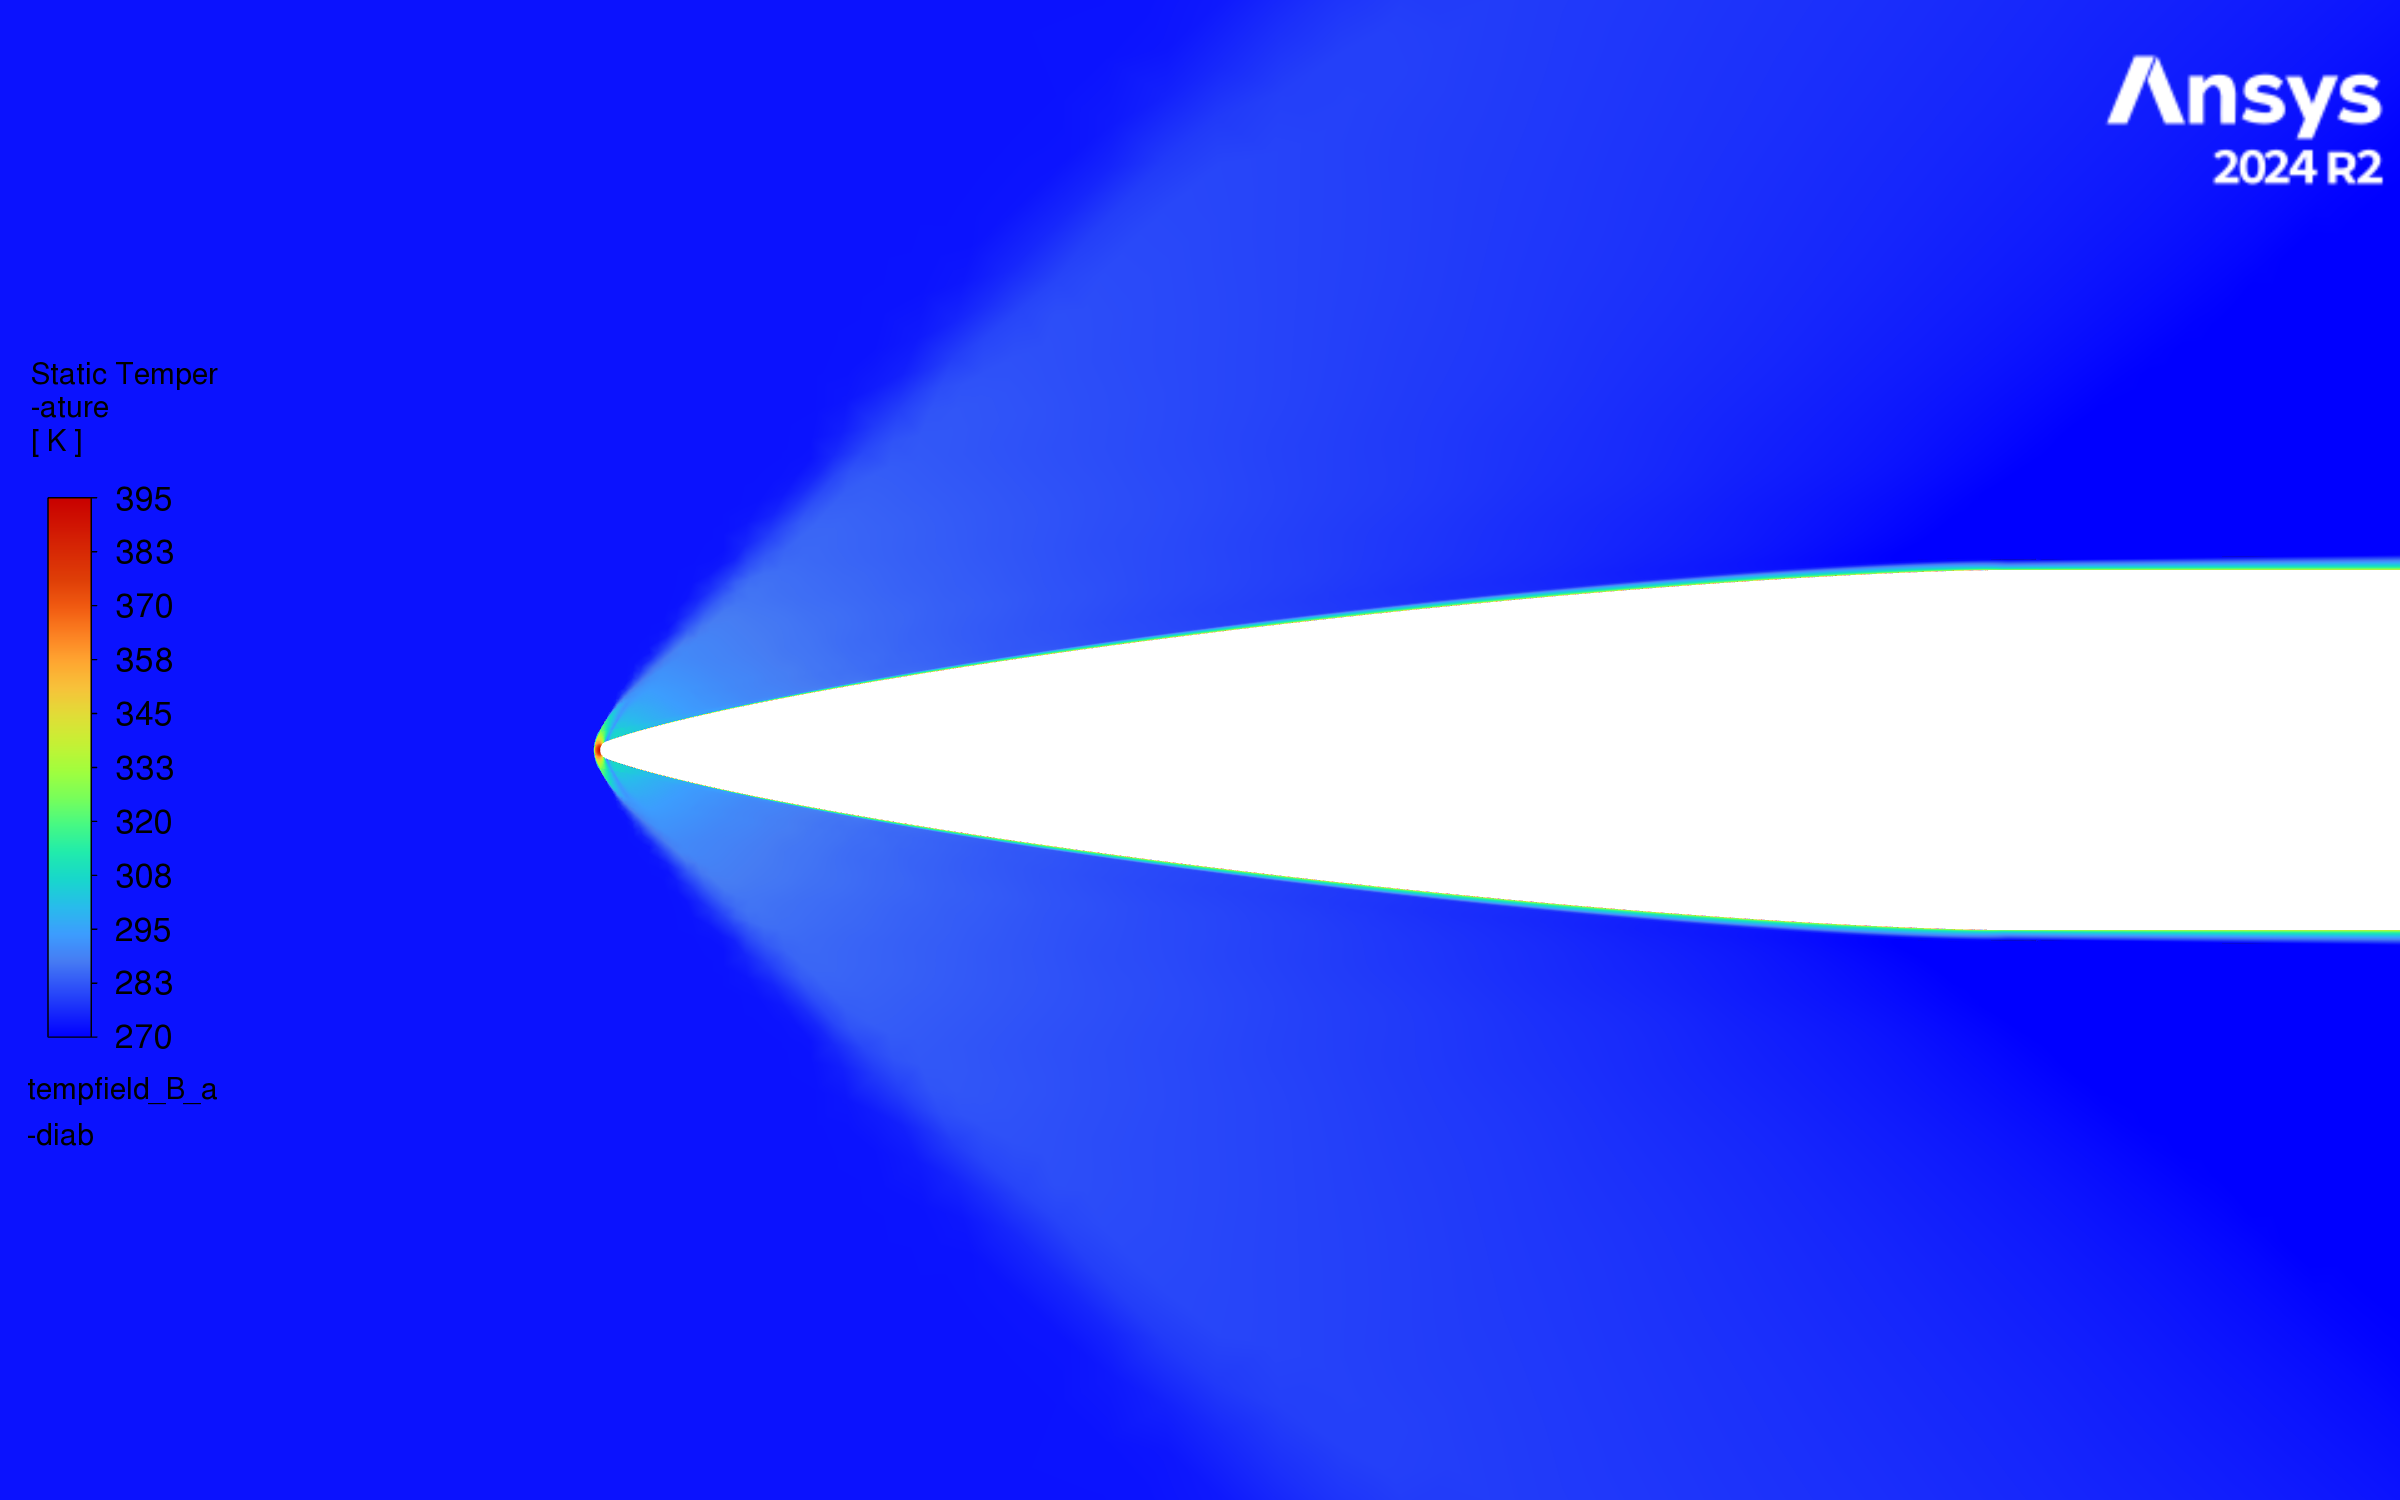
\includegraphics[width=\linewidth]{fluent_tempfield_B_adiab}
\caption{Design B.}
\end{subfigure}
\caption{Air temperature around the whole nose at burnout, adiabatic wall (Fluent). The hot air stays in a
thin layer along the wall; the light band is the air heated by the bow shock. Colour scale: 270\,K (blue) to 395\,K (red).}
\label{fig:tempfield}
\end{figure}

\begin{figure}[H]
\centering
\begin{subfigure}[t]{0.49\linewidth}
\centering
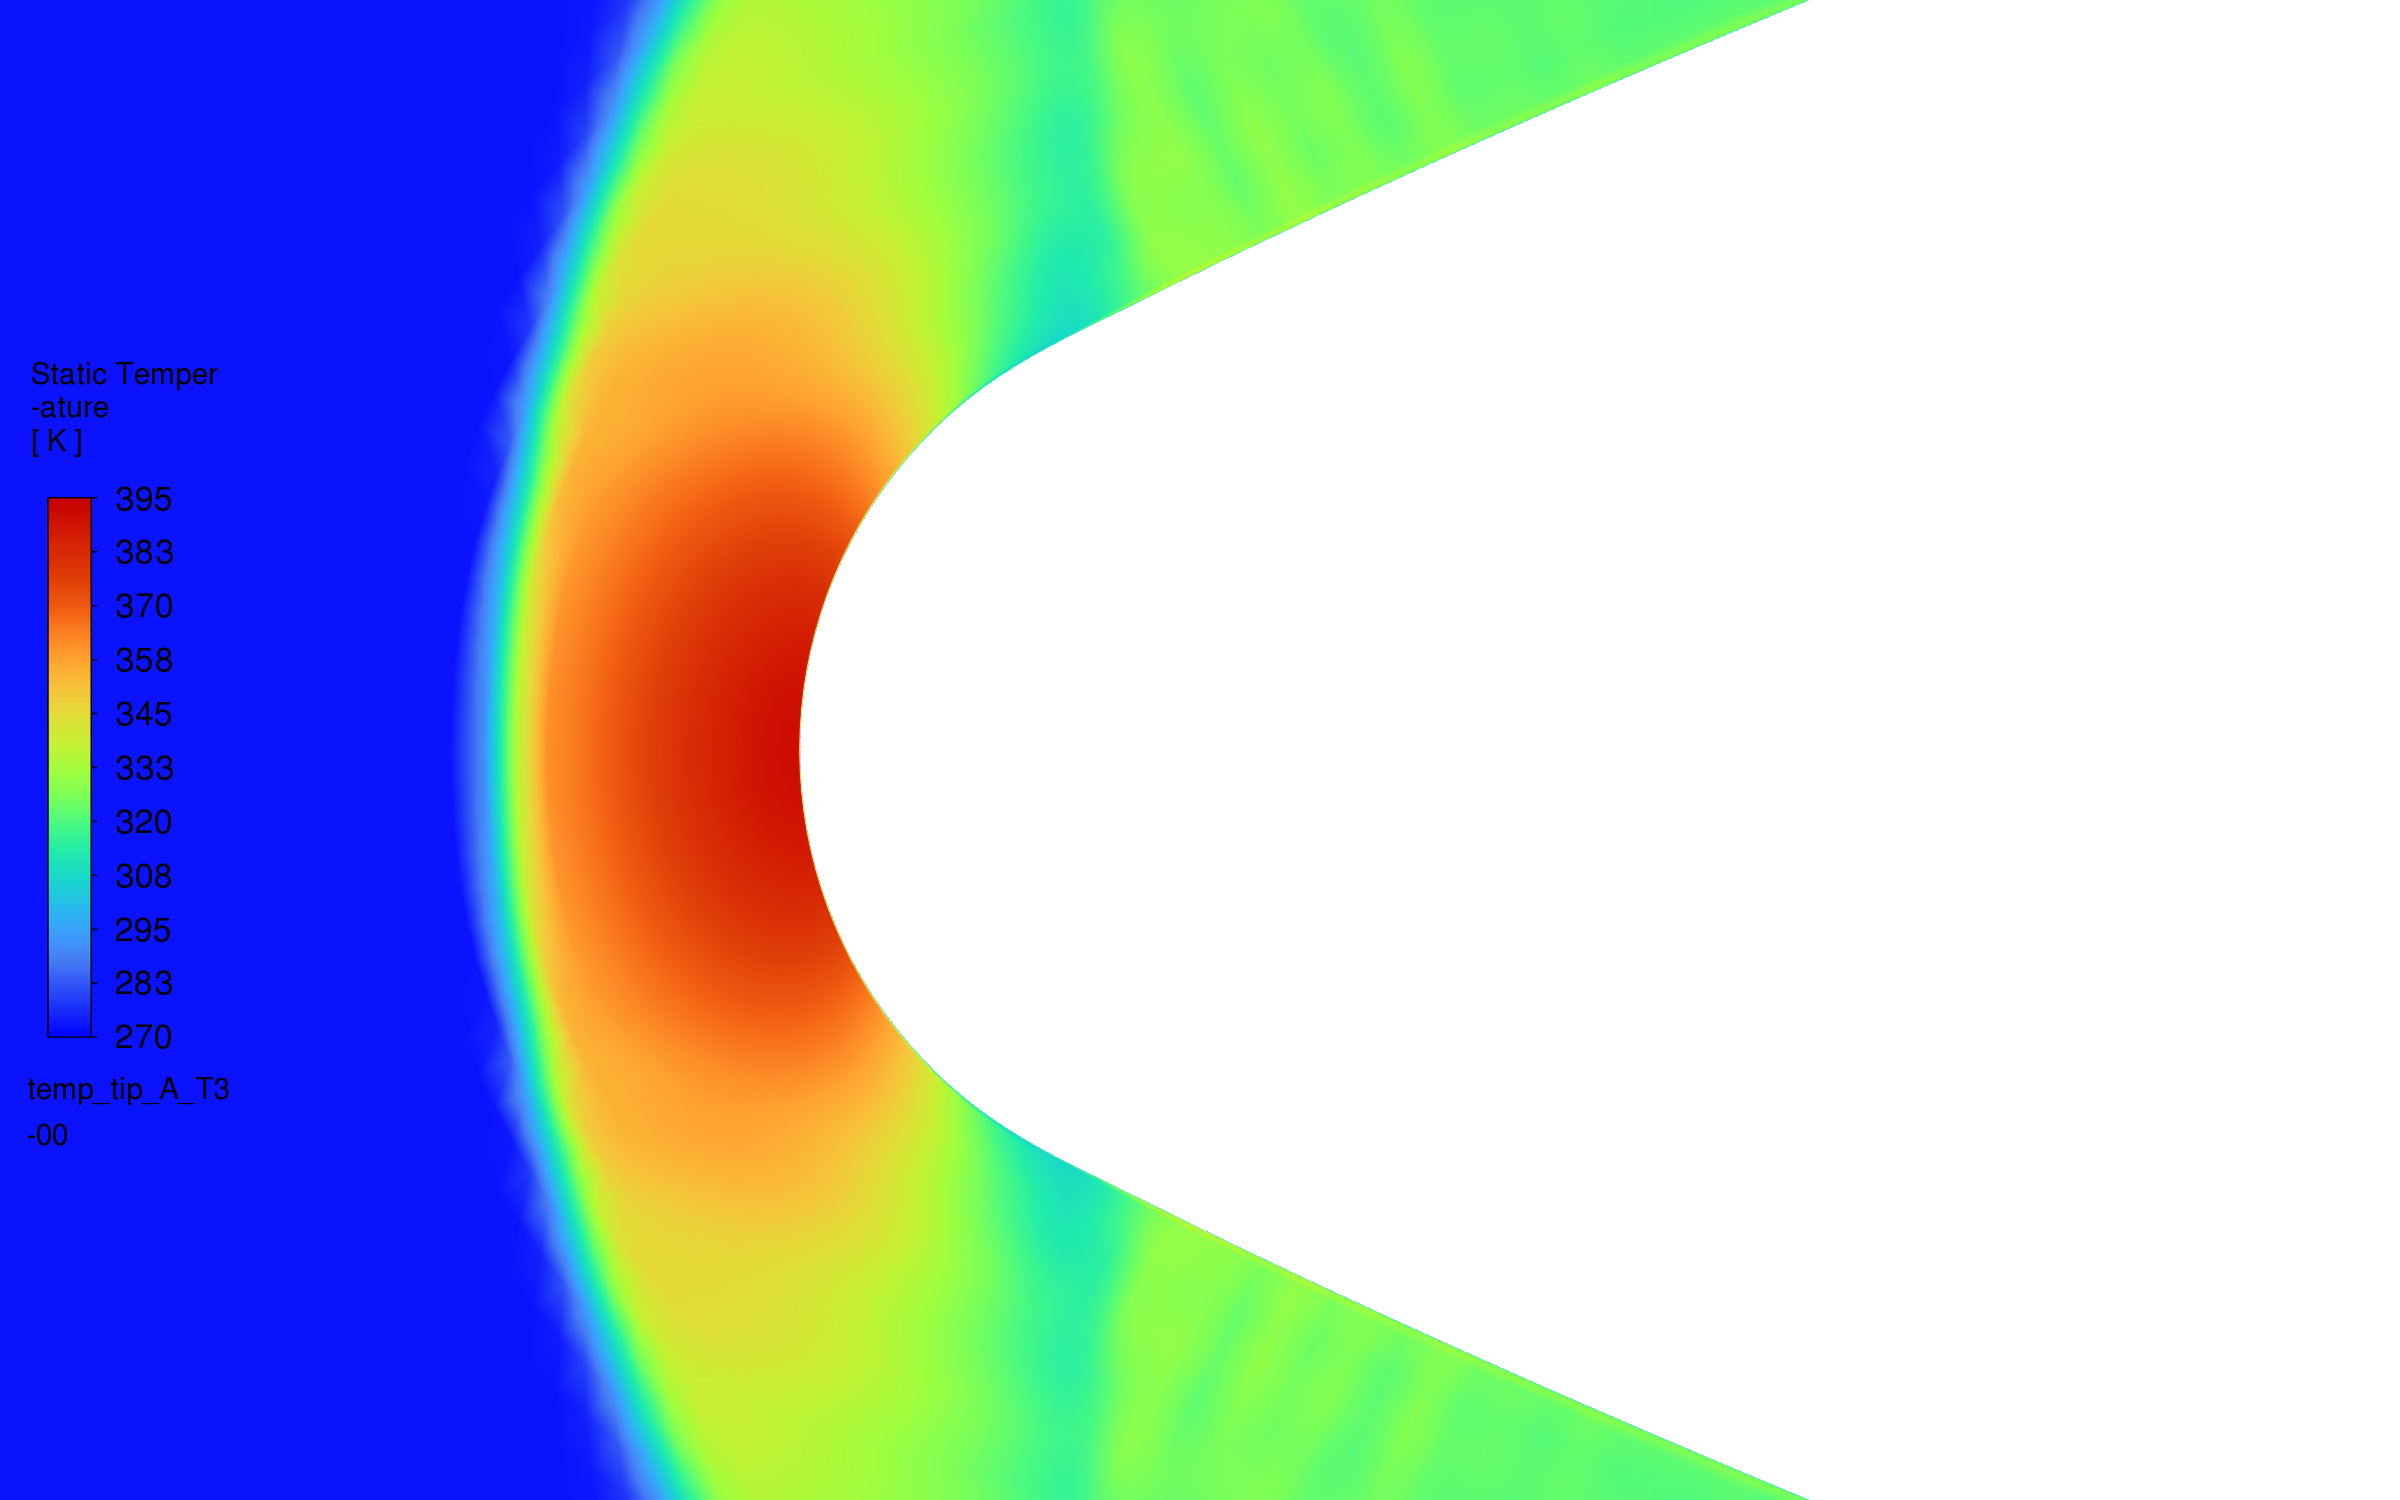
\includegraphics[width=\linewidth]{fluent_temp_tip_A_T300}
\caption{Design A.}
\end{subfigure}\hfill
\begin{subfigure}[t]{0.49\linewidth}
\centering
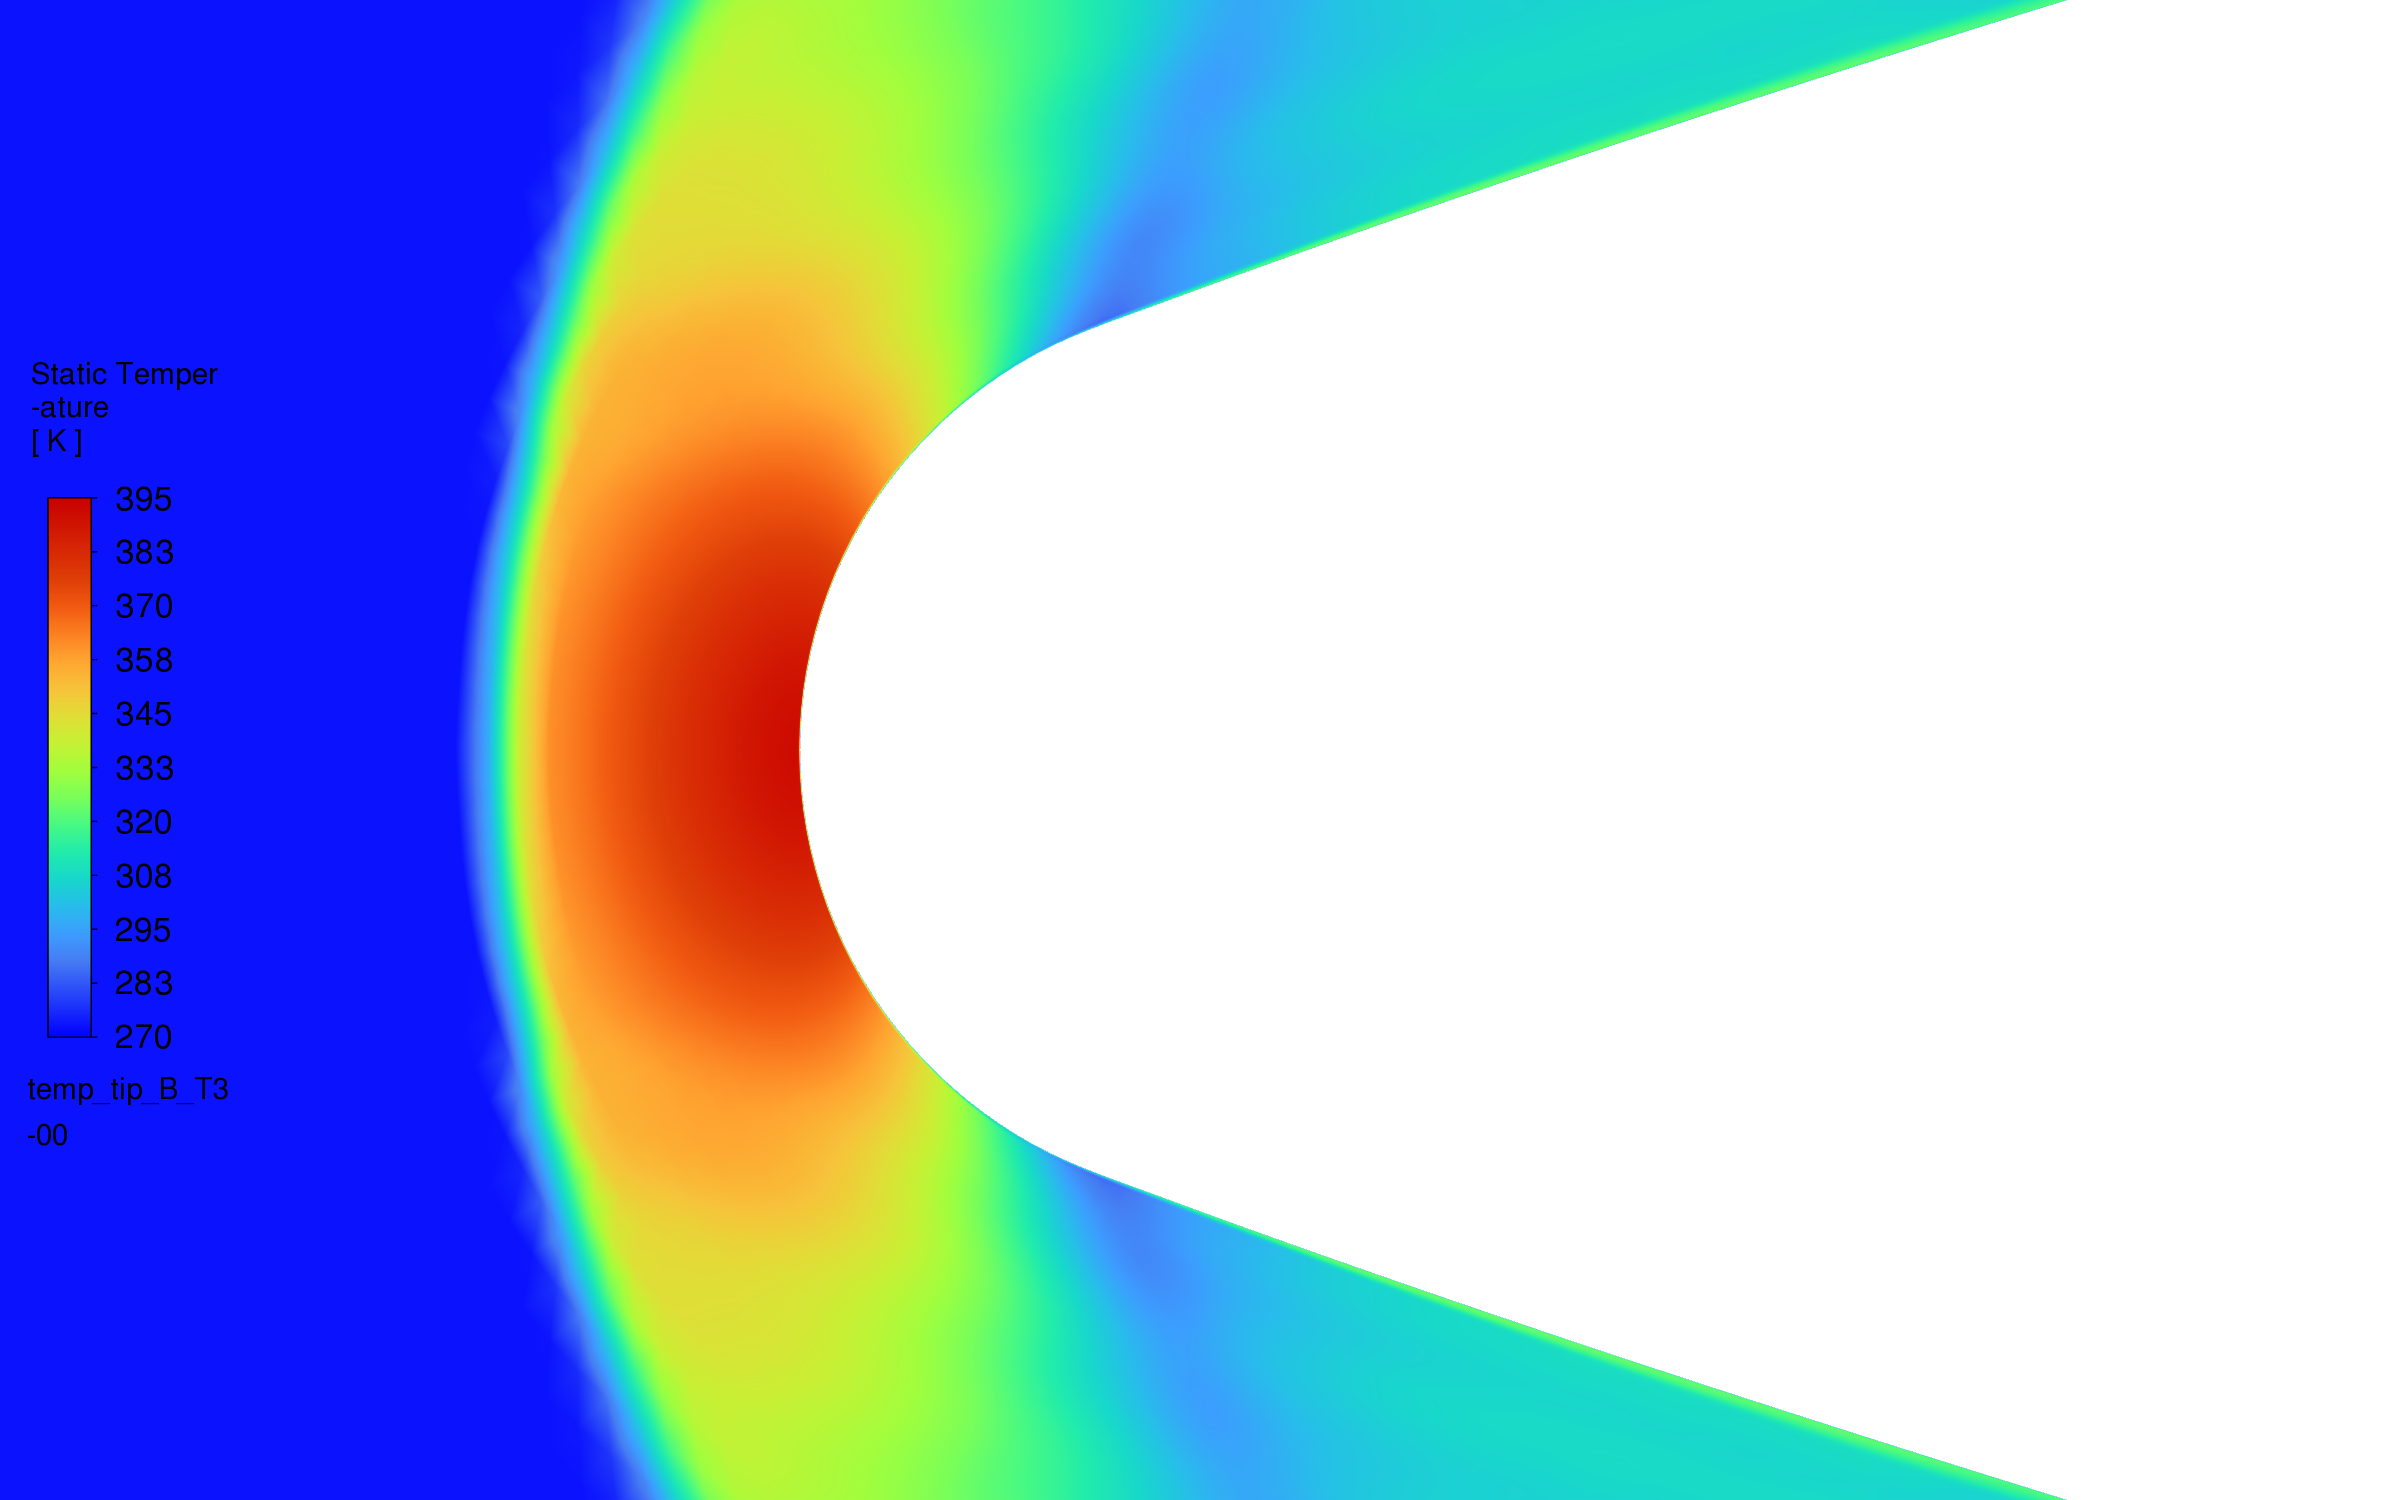
\includegraphics[width=\linewidth]{fluent_temp_tip_B_T300}
\caption{Design B.}
\end{subfigure}
\caption{Air temperature around the tip at burnout with the wall held at \SI{300}{K} (Fluent). The cold
wall cools the air next to it: this temperature drop at the wall is the heat going into the nose. Colour scale: 270\,K (blue) to 395\,K (red).}
\label{fig:tipT300}
\end{figure}

\paragraph{Heating along the wall.} Figures~\ref{fig:taw}--\ref{fig:hfluent} give the heating along the
wall of both designs, and Table~\ref{tab:fluentheat} sums it up.
\begin{itemize}
\item The \textbf{wall temperature} $T_{aw}$ is \val{A-Taw0}\,K at the tip and
\val{A-Taw-far-lo}--\val{A-Taw-far-hi}\,K further back: the whole nose is driven to about
107--110\,\si{\celsius} at burnout.
\item The \textbf{heat flux} and $h$ are highest at the tip and fall along the nose: $h$ goes from about
\SI{1900}{W/(m^2K)} at the tip to about \SI{1000}{W/(m^2K)} at 50\,mm and about \SI{550}{W/(m^2K)} at
the shoulder. So the front of the shell heats up fastest.
\item A and B differ only over the first 10\,cm, and by little. The heating does not separate the two
designs.
\end{itemize}

\begin{figure}[H]
\centering
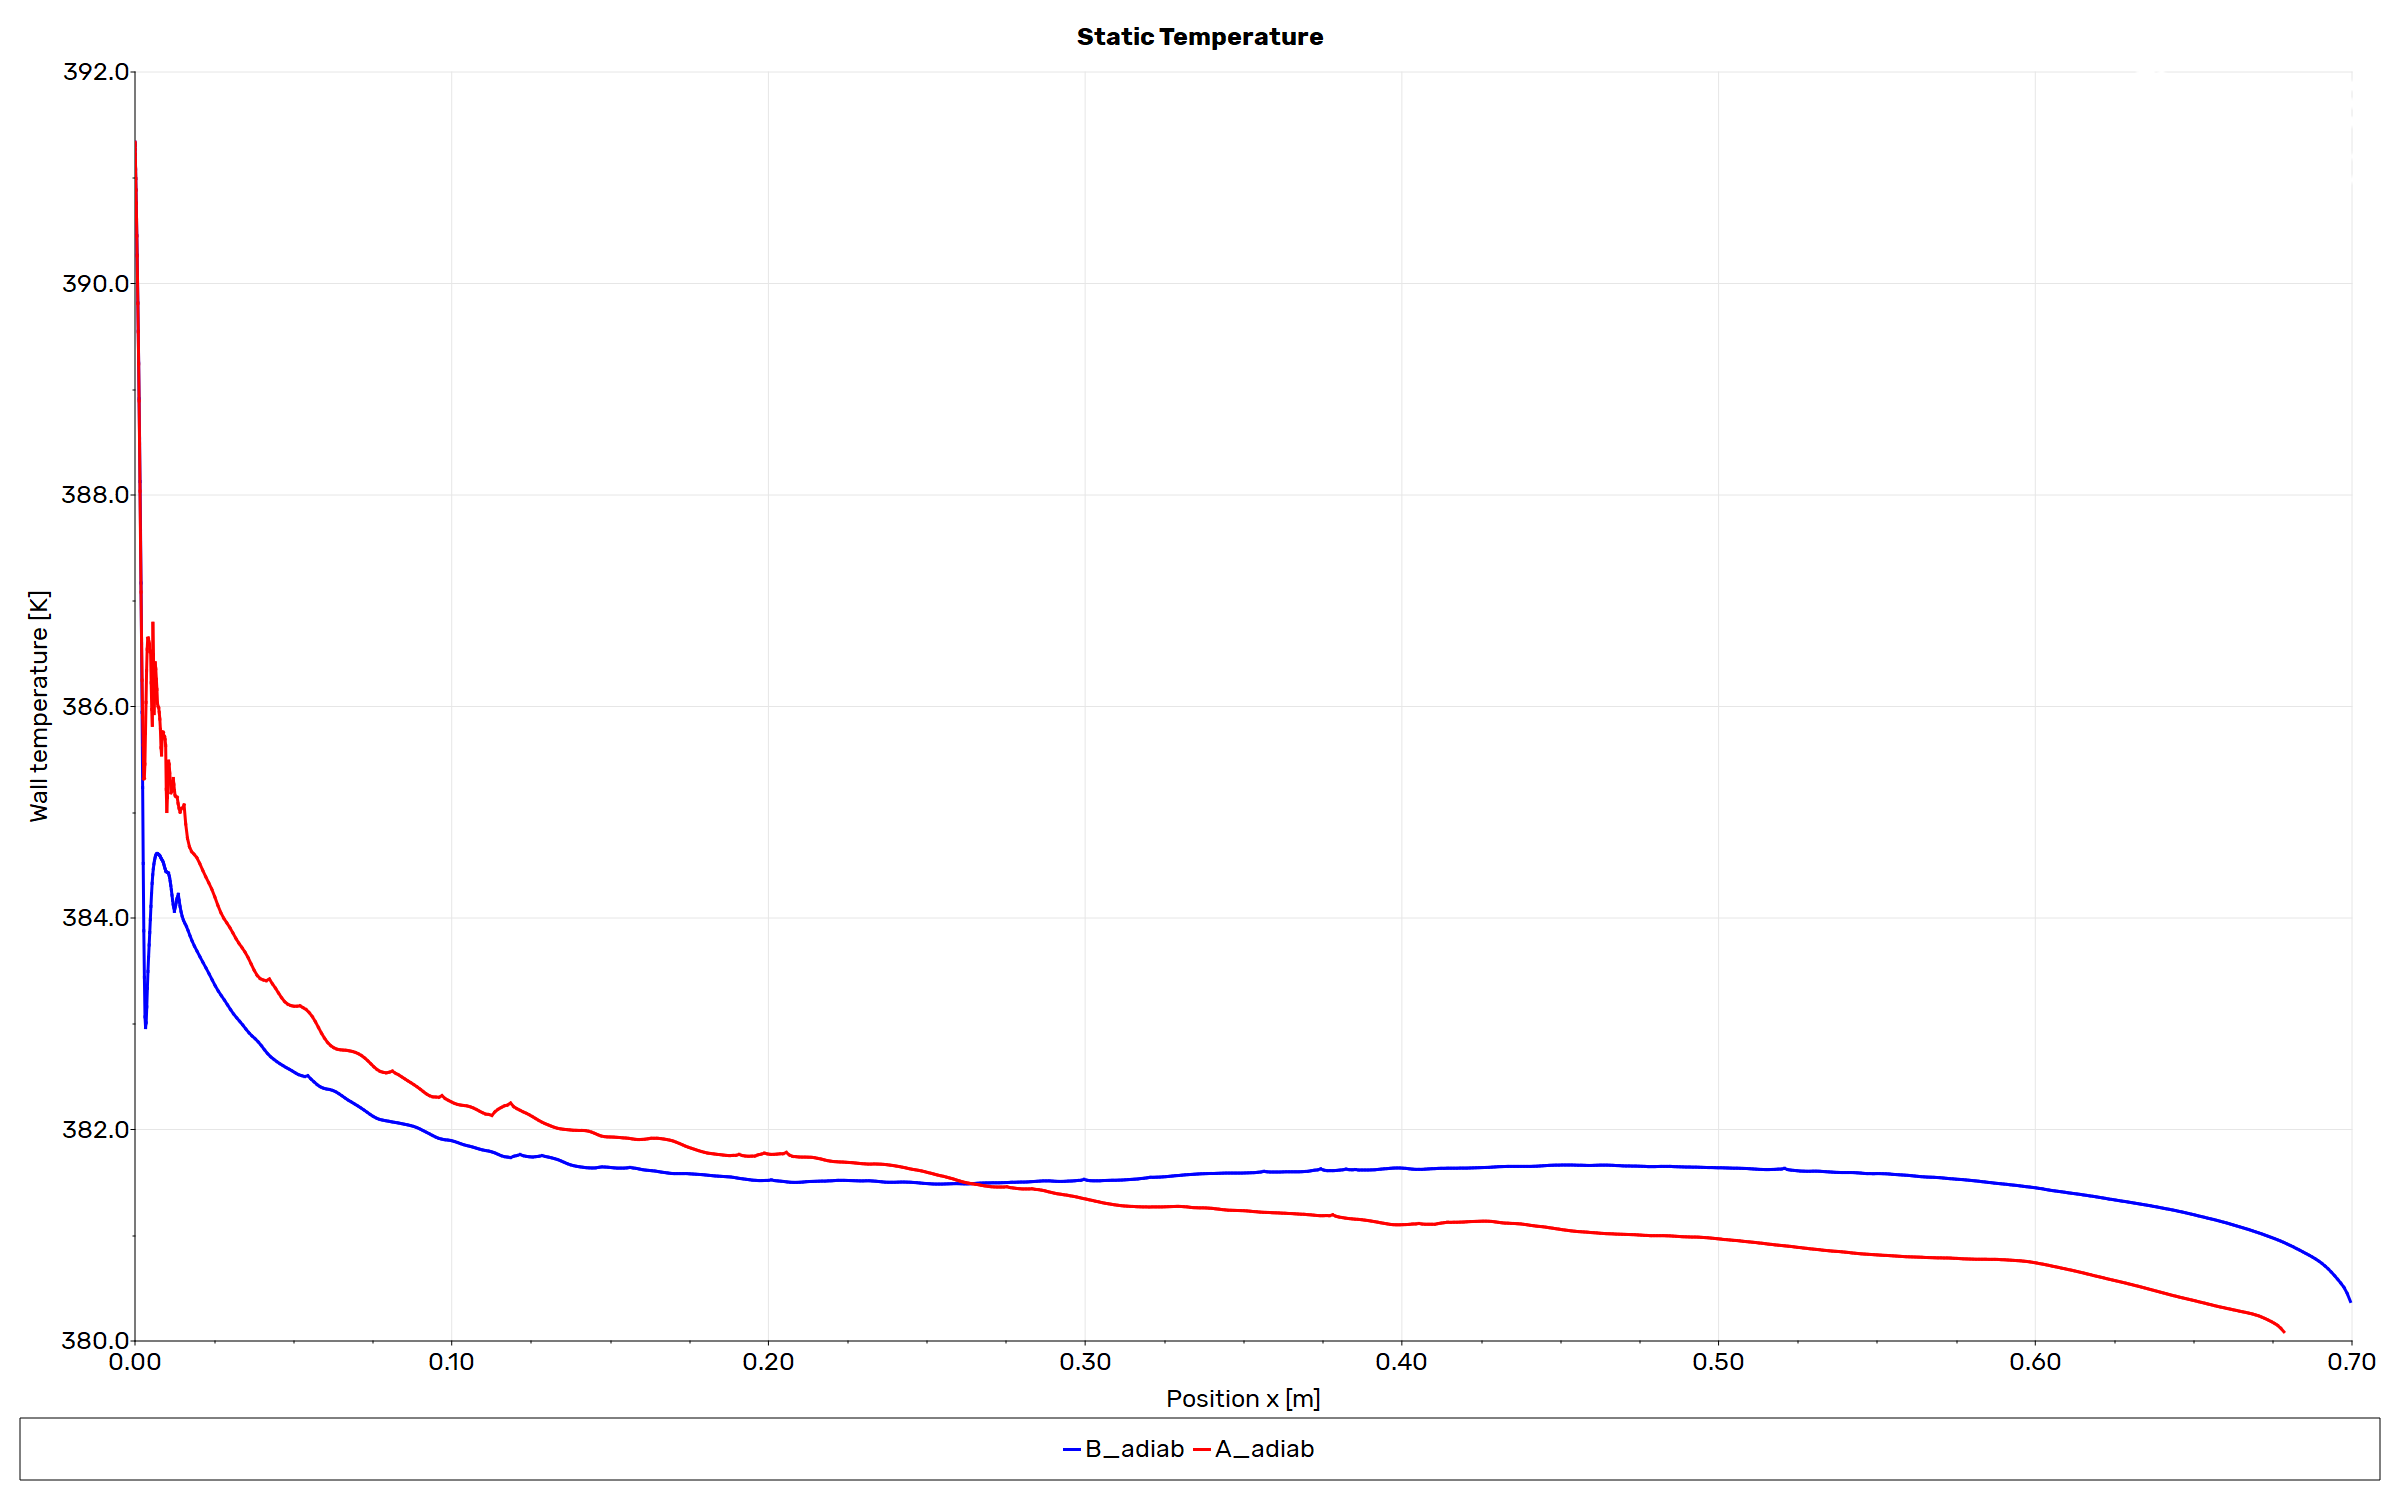
\includegraphics[width=0.9\linewidth]{fluent_twall_AB_adiab}
\caption{Adiabatic wall temperature along the nose at burnout, design A (red) and B (blue), Fluent. This
is the temperature the air drives the wall towards. The ripple over the first 15\,mm is a mesh effect,
where the fine tip cells meet the wall cells.}
\label{fig:taw}
\end{figure}

\begin{figure}[H]
\centering
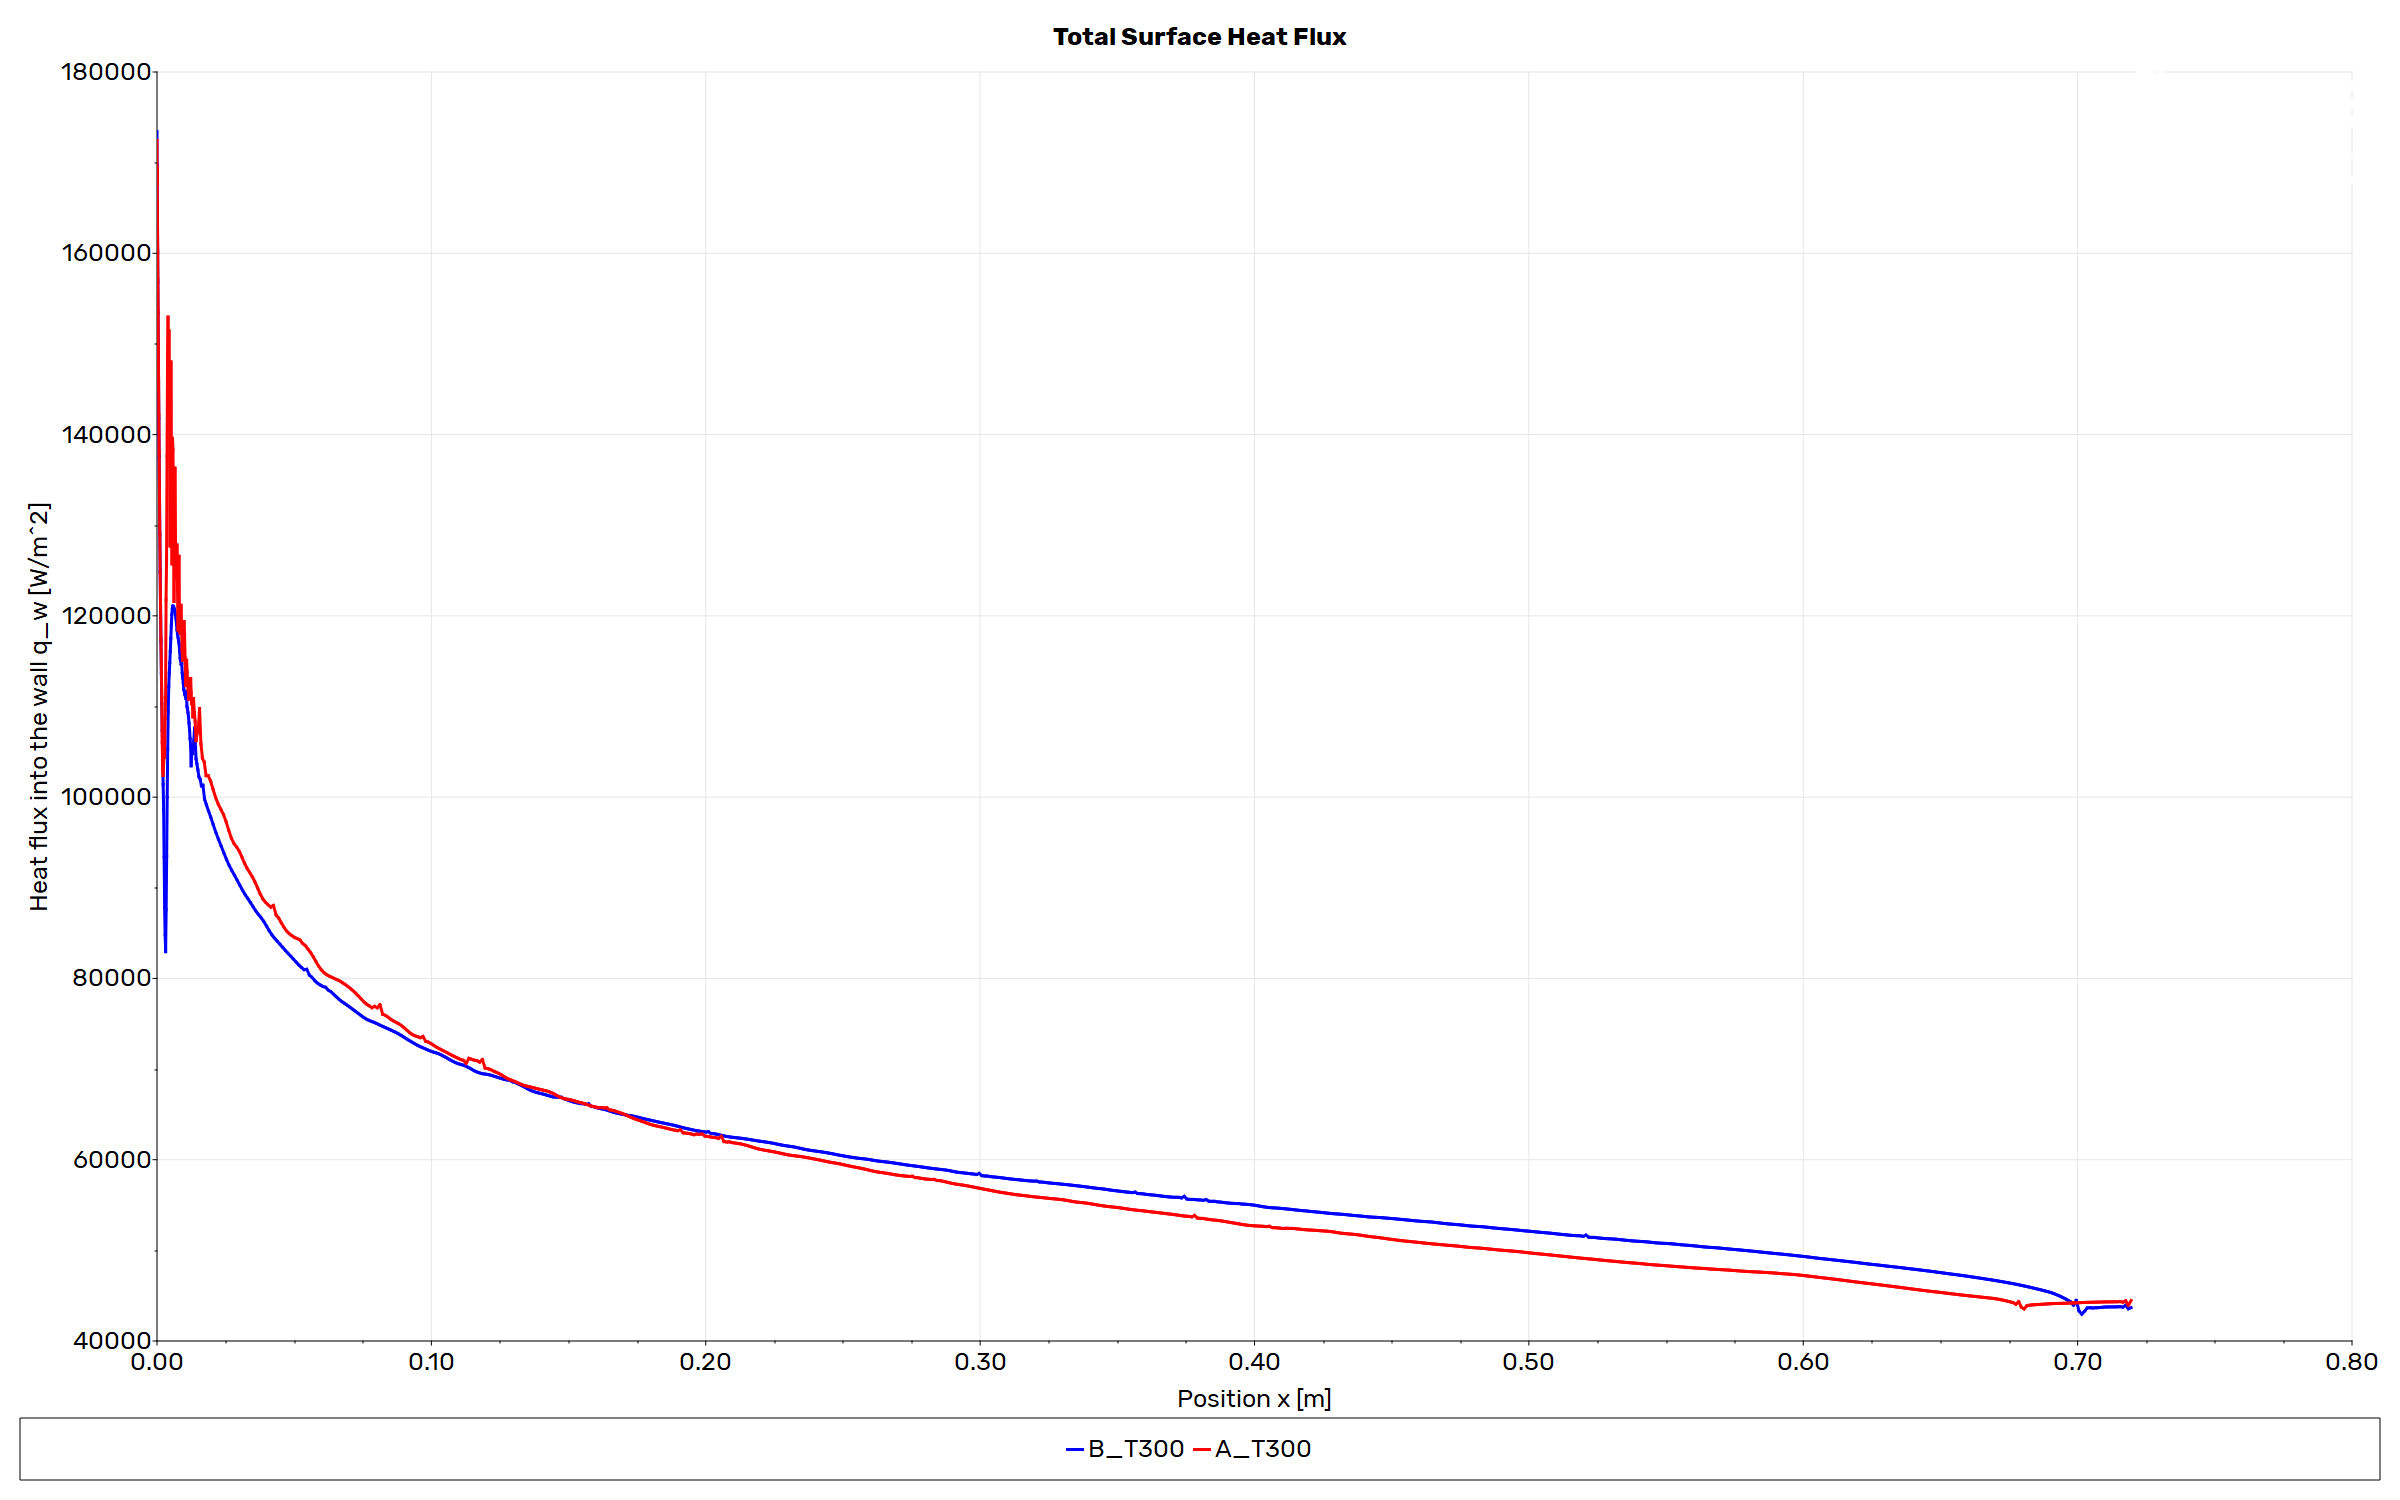
\includegraphics[width=0.9\linewidth]{fluent_qw_AB_T300}
\caption{Heat flux into a wall held at \SI{300}{K} along the nose at burnout, design A (red) and B
(blue), Fluent.}
\label{fig:qw}
\end{figure}

\begin{figure}[H]
\centering
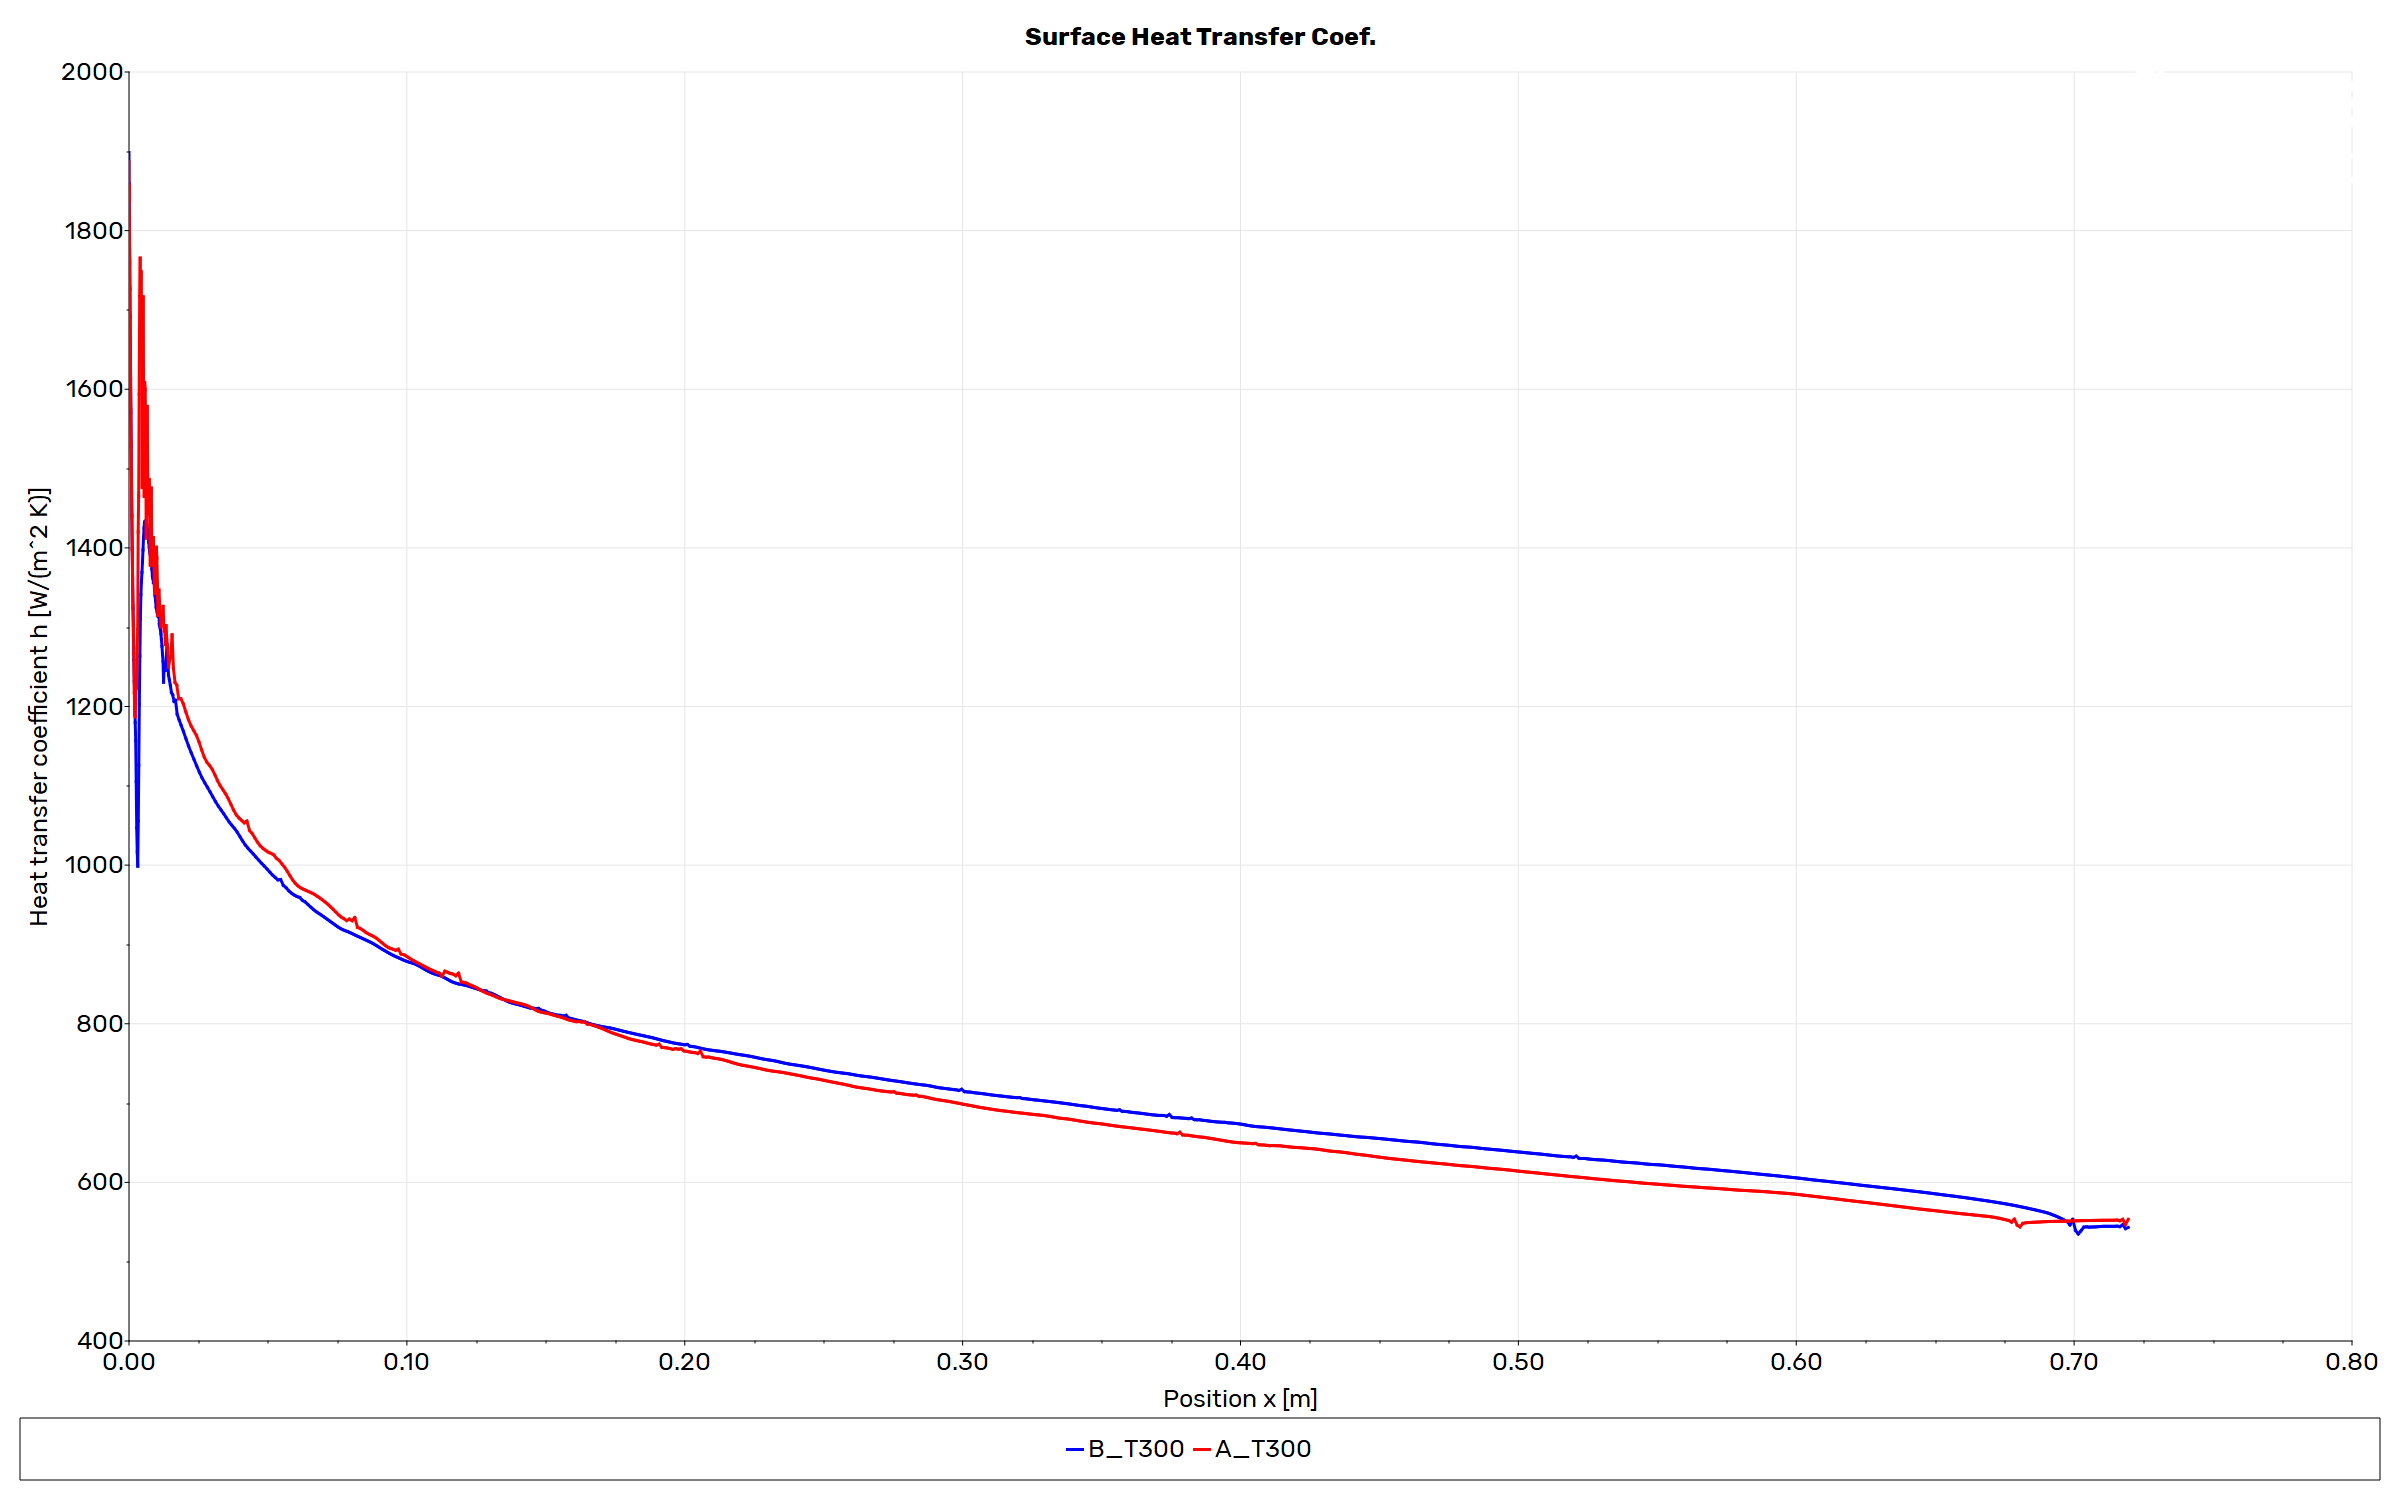
\includegraphics[width=0.9\linewidth]{fluent_h_AB_T300}
\caption{Heat-transfer coefficient $h = q_w / (T_{aw} - \SI{300}{K})$ along the nose at burnout, design A
(red) and B (blue), Fluent. This is the input of the shell model.}
\label{fig:hfluent}
\end{figure}

\begin{table}[H]
\centering
\caption{Heating at burnout from Fluent, nominal day.}
\label{tab:fluentheat}
\small
\begin{tabular}{@{}llcc@{}}
\toprule
 & Unit & Design A & Design B\\
\midrule
Stagnation temperature of the air & K & \val{T0-burnout} & \val{T0-burnout}\\
Wall temperature (adiabatic) at the tip & K & \val{A-Taw0} & \val{B-Taw0}\\
Wall temperature (adiabatic) beyond 50\,mm & K & \val{A-Taw-far-lo}--\val{A-Taw-far-hi} & \val{B-Taw-far-lo}--\val{B-Taw-far-hi}\\
Heat flux at the tip, wall at \SI{300}{K} & kW/m$^2$ & \val{A-qw0} & \val{B-qw0}\\
Heat-transfer coefficient $h$ at the tip & W/(m$^2$K) & \val{A-h0} & \val{B-h0}\\
Heat-transfer coefficient $h$ at the shoulder & W/(m$^2$K) & \val{A-hS} & \val{B-hS}\\
\bottomrule
\end{tabular}
\end{table}

\subsection{Temperature profile along the nose}

Fluent gives the heating at burnout only. To follow the temperatures through the whole flight, the
Python model of report~1 is used, with its heating calibrated on Fluent (Appendix~\ref{app:heatmethod}).
It computes the heat conduction through the \val{shell-t}\,mm CFRP shell at stations from 10\,mm to the
shoulder, heated on the outside. Two simplifications make the shell temperatures slightly high: no heat
is lost on the inside, and over the first 80\,mm the aluminium tip insert under the shell is ignored.

Figure~\ref{fig:thprofile} gives the \textbf{highest temperature reached during the flight} at every point
of the nose, and Figure~\ref{fig:thmap} shows \textbf{when and where} the shell is hot.
\begin{itemize}
\item Both faces are hottest near the tip and cool towards the shoulder, because $h$ falls along the nose.
\item The outer face stays below the DP490 limit everywhere. The inner face is above Req\_10 everywhere.
\item The inner face lags the outer face by about 2\,s, because the heat needs time to cross the CFRP.
Req\_10 is exceeded from about \val{th-A-nominal-req10-t0}\,s to \val{th-A-nominal-req10-t1}\,s on a
nominal day, and from \val{th-A-hot-req10-t0}\,s to \val{th-A-hot-req10-t1}\,s on a hot day.
\end{itemize}

\begin{figure}[H]
\centering
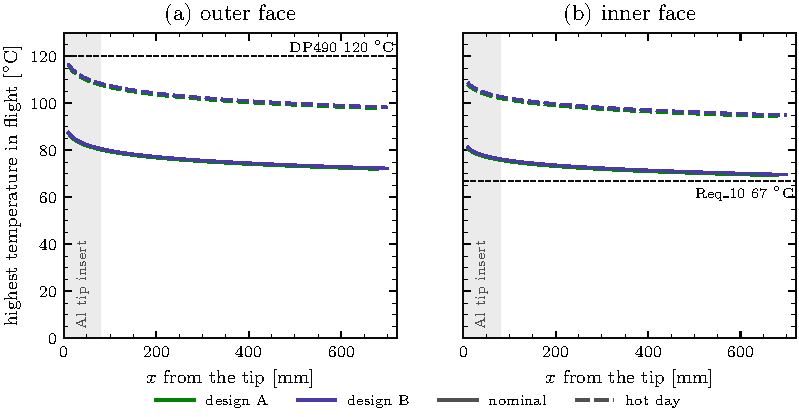
\includegraphics[width=\linewidth]{fig_thermal_profile}
\caption{Highest temperature of the shell during the flight, along the nose: (a) outer face, (b) inner
face. Design A in green, B in purple; solid: nominal day, dashed: hot day. Grey band: the first 80\,mm,
where the aluminium tip insert sits under the shell.}
\label{fig:thprofile}
\end{figure}

\begin{figure}[H]
\centering
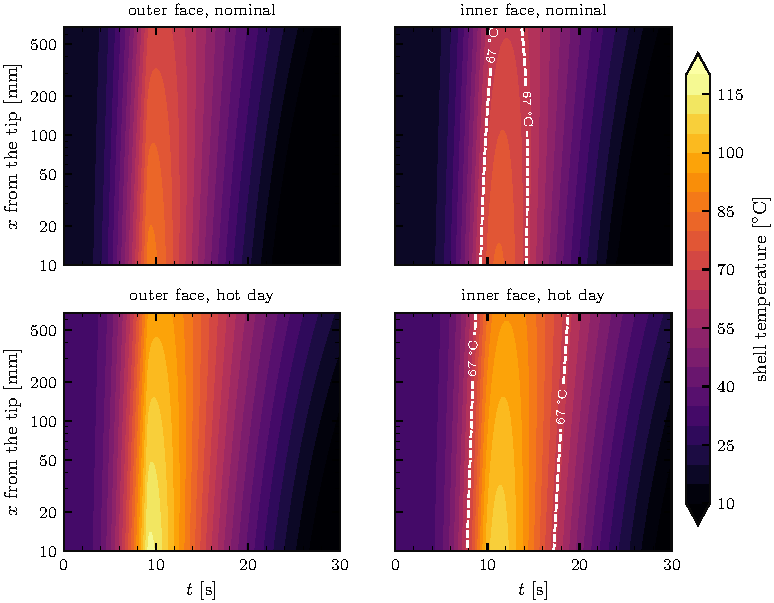
\includegraphics[width=0.8\linewidth]{fig_thermal_map}
\caption{Shell temperature of design A against time and position. Left: outer face; right: inner face.
Top: nominal day; bottom: hot day. White dashed line: \SI{67}{\celsius} (Req\_10) on the inner face. The outer face
stays below \SI{120}{\celsius} (DP490), so it has no line. Design B is the same within \val{th-AB-diff}\,\si{\celsius}.}
\label{fig:thmap}
\end{figure}

\begin{table}[H]
\centering
\caption{Highest shell temperature during the flight at four stations [\si{\celsius}]. \ok: below the limit; \bad: above it.}
\label{tab:thstations}
\small
\begin{tabular}{@{}lccccc@{}}
\toprule
 & \multicolumn{2}{c}{Design A} & \multicolumn{2}{c}{Design B} & \\
\cmidrule(lr){2-3}\cmidrule(lr){4-5}
 & Nominal & Hot day & Nominal & Hot day & Limit\\
\midrule
\grouprow{6}{Outer face}
20\,mm & \val{th-A-nominal-Tout-20} & \val{th-A-hot-Tout-20} & \val{th-B-nominal-Tout-20} & \val{th-B-hot-Tout-20} & 120 (DP490) \ok\\
50\,mm & \val{A-nominal-Tout50} & \val{A-hot-Tout50} & \val{B-nominal-Tout50} & \val{B-hot-Tout50} & 120 (DP490) \ok\\
Mid-length & \val{th-A-nominal-Tout-mid} & \val{th-A-hot-Tout-mid} & \val{th-B-nominal-Tout-mid} & \val{th-B-hot-Tout-mid} & 120 (DP490) \ok\\
Shoulder & \val{th-A-nominal-Tout-shoulder} & \val{th-A-hot-Tout-shoulder} & \val{th-B-nominal-Tout-shoulder} & \val{th-B-hot-Tout-shoulder} & 120 (DP490) \ok\\
\midrule
\grouprow{6}{Inner face}
20\,mm & \val{th-A-nominal-Tin-20} & \val{th-A-hot-Tin-20} & \val{th-B-nominal-Tin-20} & \val{th-B-hot-Tin-20} & 67 (Req\_10) \bad\\
50\,mm & \val{A-nominal-Tin50} & \val{A-hot-Tin50} & \val{B-nominal-Tin50} & \val{B-hot-Tin50} & 67 (Req\_10) \bad\\
Mid-length & \val{th-A-nominal-Tin-mid} & \val{th-A-hot-Tin-mid} & \val{th-B-nominal-Tin-mid} & \val{th-B-hot-Tin-mid} & 67 (Req\_10) \bad\\
Shoulder & \val{th-A-nominal-Tin-shoulder} & \val{th-A-hot-Tin-shoulder} & \val{th-B-nominal-Tin-shoulder} & \val{th-B-hot-Tin-shoulder} & 67 (Req\_10) \bad\\
\bottomrule
\end{tabular}
\end{table}

\subsection{Temperatures during the flight}

Figure~\ref{fig:temps} follows the parts that matter most for ST through the flight: the aluminium tip
insert, the shell at 50\,mm (inside the region of the insert) and the air inside the nose. The peaks of
the tip insert and the inside air are in Table~\ref{tab:heat}, those of the shell in
Table~\ref{tab:thstations}.
\begin{itemize}
\item The outer face of the shell peaks just after burnout (9.6\,s), the inner face 2\,s later.
\item The tip insert, with its larger heat capacity, peaks later, at 12--13\,s, and cools slowly.
\item The tip insert of design B gets \SI{20}{\percent} less heat than A's (its front is thinner, so there
is less surface in the first 80\,mm) and stays 5--6\,\si{\celsius} cooler.
\item The air inside follows the inner face of the shell (upper bound). Whether Req\_10 applies to the air or
to the inner wall is still open with SE.
\end{itemize}

\begin{figure}[H]
\centering
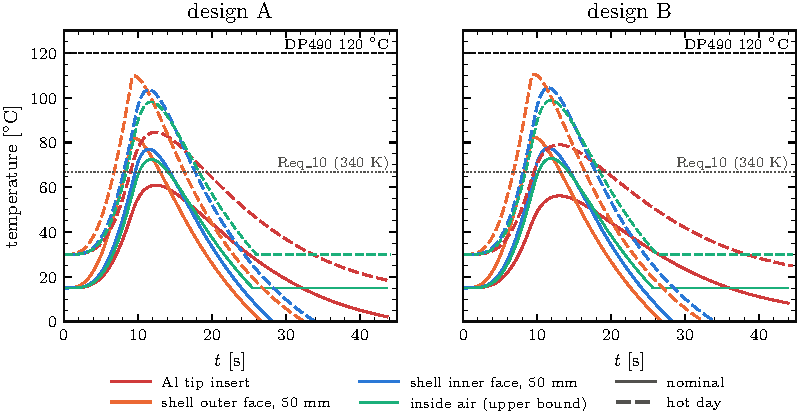
\includegraphics[width=\linewidth]{fig_temperatures}
\caption{Temperatures during the flight, design A (a) and B (b): aluminium tip insert, CFRP shell at
50\,mm (outer and inner face) and the inside air (upper bound). Solid: nominal day; dashed: hot day.}
\label{fig:temps}
\end{figure}

\begin{table}[H]
\centering
\caption{Highest stagnation, tip-insert and inside-air temperatures during the flight (the shell is
in Table~\ref{tab:thstations}). \bad: above the limit. Tip insert: Al\,6082, \val{tip-mass}\,g over the first
\val{tip-length}\,mm.}
\label{tab:heat}
\small
\begin{tabular}{@{}llccccc@{}}
\toprule
 & & \multicolumn{2}{c}{Design A} & \multicolumn{2}{c}{Design B} & \\
\cmidrule(lr){3-4}\cmidrule(lr){5-6}
 & Unit & Nominal & Hot day & Nominal & Hot day & Limit\\
\midrule
Stagnation temperature of the air & \si{\celsius} & \val{A-nominal-T0} & \val{A-hot-T0} & \val{B-nominal-T0} & \val{B-hot-T0} & \\
Aluminium tip insert & \si{\celsius} & \val{A-nominal-Ttip} & \val{A-hot-Ttip} & \val{B-nominal-Ttip} & \val{B-hot-Ttip} & \\
Inside air, upper bound & \si{\celsius} & \val{A-nominal-Tair} & \val{A-hot-Tair} & \val{B-nominal-Tair} & \val{B-hot-Tair} & 67 (Req\_10) \bad\\
\bottomrule
\end{tabular}
\end{table}


\clearpage
\section{Drag: design A against design B}
\label{sec:drag}

\begin{keybox}
\begin{itemize}
\item \textbf{Below Mach 1 the two noses have the same drag.} About \SI{90}{\percent} of it is skin
friction, which depends on the wetted surface, and that is almost the same for both.
\item \textbf{Above Mach 1 design B has \val{BlessA-M120} to \val{BlessA-M147}\,\% less drag.} The drag
is then mostly shock (wave) drag, which comes from the front of the nose, and B's front is thinner.
\item At burnout Fluent gives \val{A-F-M147}\,N for A and \val{B-F-M147}\,N for B. In flight, with a
rough wall, the drag peaks at \val{A-nominal-Dnmax}\,N (A) and \val{B-nominal-Dnmax}\,N (B),
\val{A-hot-Dnmax} and \val{B-hot-Dnmax}\,N on a hot day.
\item The lower drag gives B a higher apogee: \val{B-apogee}\,m against \val{A-apogee}\,m (nominal day).
\end{itemize}
\end{keybox}

\subsection{Drag at the three Fluent points}

\begin{table}[H]
\centering
\caption{Drag of the nose from Fluent [N], smooth wall. Pressure: the pressure drag of the curved part,
mostly wave drag above Mach 1. The coupler only has friction. $C_D$: drag coefficient of the curved part,
on $A_{ref} = \pi R^2$.}
\label{tab:forces}
\small
\begin{tabular}{@{}lcccccc@{}}
\toprule
 & \multicolumn{2}{c}{$M = 0.95$} & \multicolumn{2}{c}{$M = 1.20$} & \multicolumn{2}{c}{Burnout, $M = \val{pt-M147-M}$}\\
\cmidrule(lr){2-3}\cmidrule(lr){4-5}\cmidrule(l){6-7}
 & A & B & A & B & A & B\\
\midrule
Pressure drag, nose & \val{A-Fp-M095} & \val{B-Fp-M095} & \val{A-Fp-M120} & \val{B-Fp-M120} & \val{A-Fp-M147} & \val{B-Fp-M147}\\
Friction, nose & \val{A-Fv-M095} & \val{B-Fv-M095} & \val{A-Fv-M120} & \val{B-Fv-M120} & \val{A-Fv-M147} & \val{B-Fv-M147}\\
Friction, coupler & \val{A-Fc-M095} & \val{B-Fc-M095} & \val{A-Fc-M120} & \val{B-Fc-M120} & \val{A-Fc-M147} & \val{B-Fc-M147}\\
\textbf{Total} & \textbf{\val{A-F-M095}} & \textbf{\val{B-F-M095}} & \textbf{\val{A-F-M120}} & \textbf{\val{B-F-M120}} & \textbf{\val{A-F-M147}} & \textbf{\val{B-F-M147}}\\
\midrule
$C_D$ of the nose & \val{A-cd-M095} & \val{B-cd-M095} & \val{A-cd-M120} & \val{B-cd-M120} & \val{A-cd-M147} & \val{B-cd-M147}\\
B against A & \multicolumn{2}{c}{\val{BvsA-M095}\,\%} & \multicolumn{2}{c}{\val{BvsA-M120}\,\%} & \multicolumn{2}{c}{\val{BvsA-M147}\,\%}\\
\bottomrule
\end{tabular}
\end{table}

\subsection{Why B has less drag: the flow at burnout}

At burnout a bow shock stands in front of each tip and the air slows down around the front of the nose
(Figures~\ref{fig:mach} and~\ref{fig:machtip}). The fuller front of design A slows the air more: it keeps a
higher pressure on the front of the nose (Figure~\ref{fig:cpfield}), and this pressure, acting on the
forward-facing surface, is the wave drag. Over the first centimetres A has about twice the pressure of B
(Figure~\ref{fig:cp}). Further back both noses are close to the outside pressure, and slightly below it
towards the shoulder, where the air speeds up onto the cylinder.

\begin{figure}[H]
\centering
\begin{subfigure}[t]{0.49\linewidth}
\centering
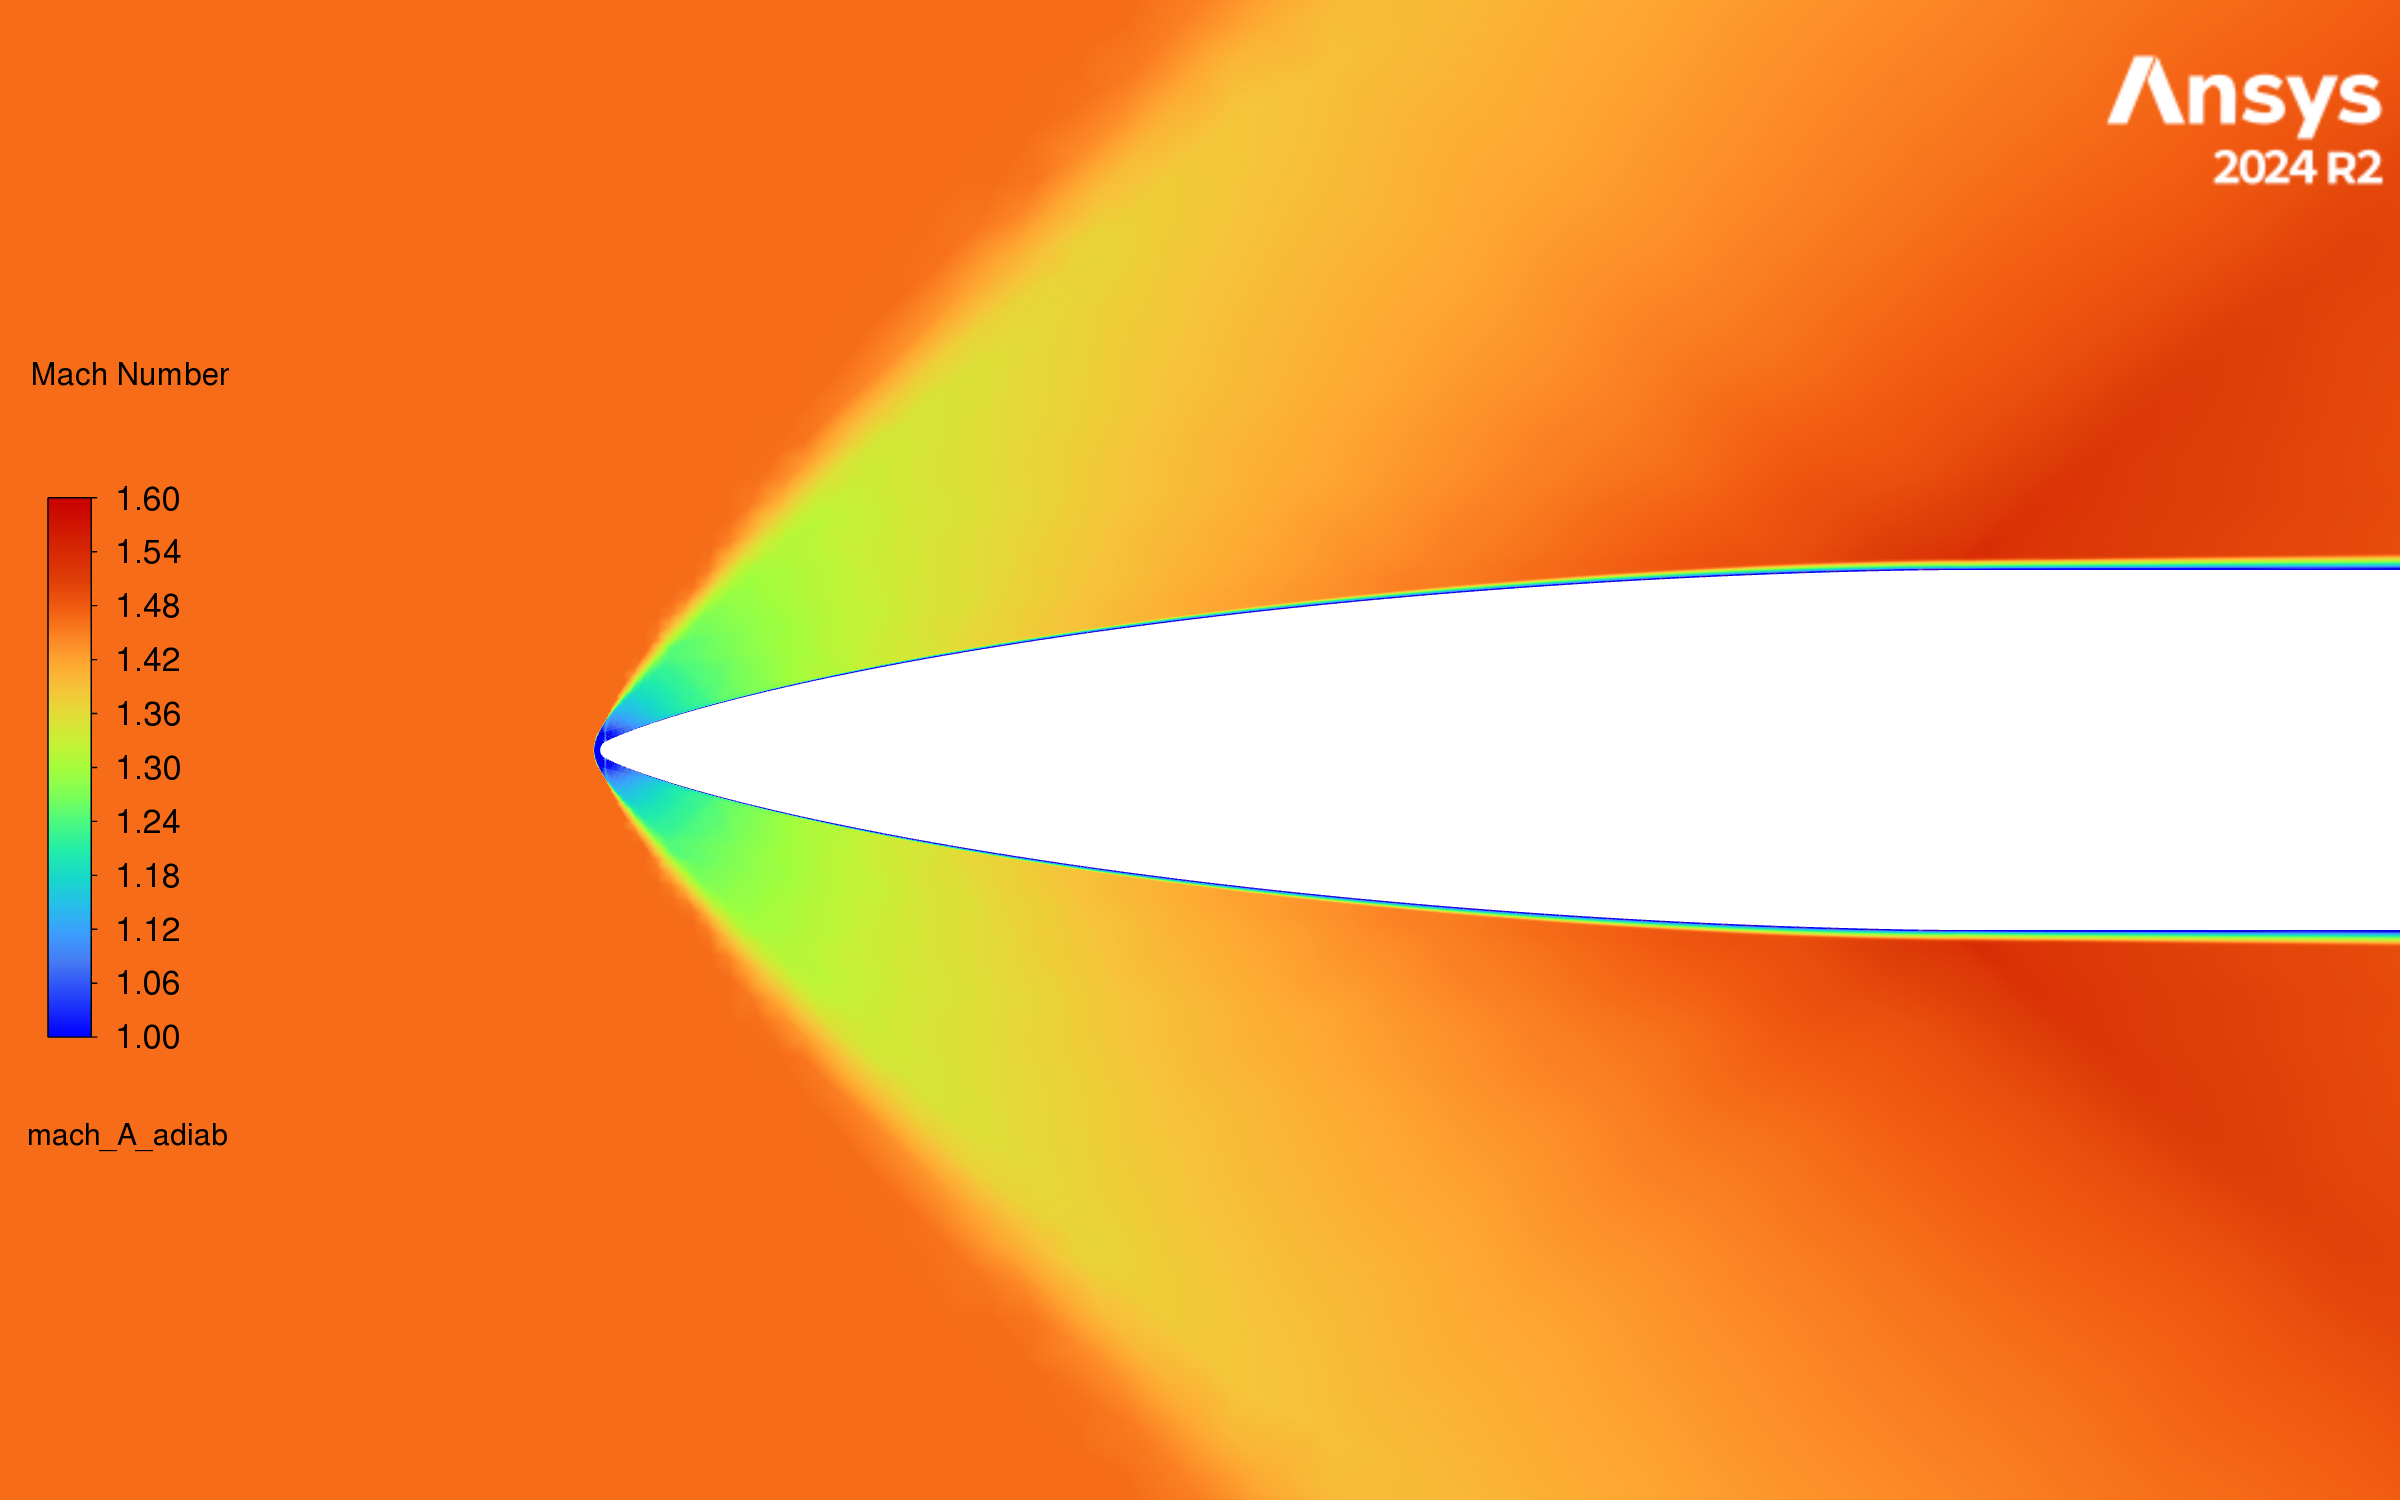
\includegraphics[width=\linewidth]{fluent_mach_A_adiab}
\caption{Design A.}
\end{subfigure}\hfill
\begin{subfigure}[t]{0.49\linewidth}
\centering
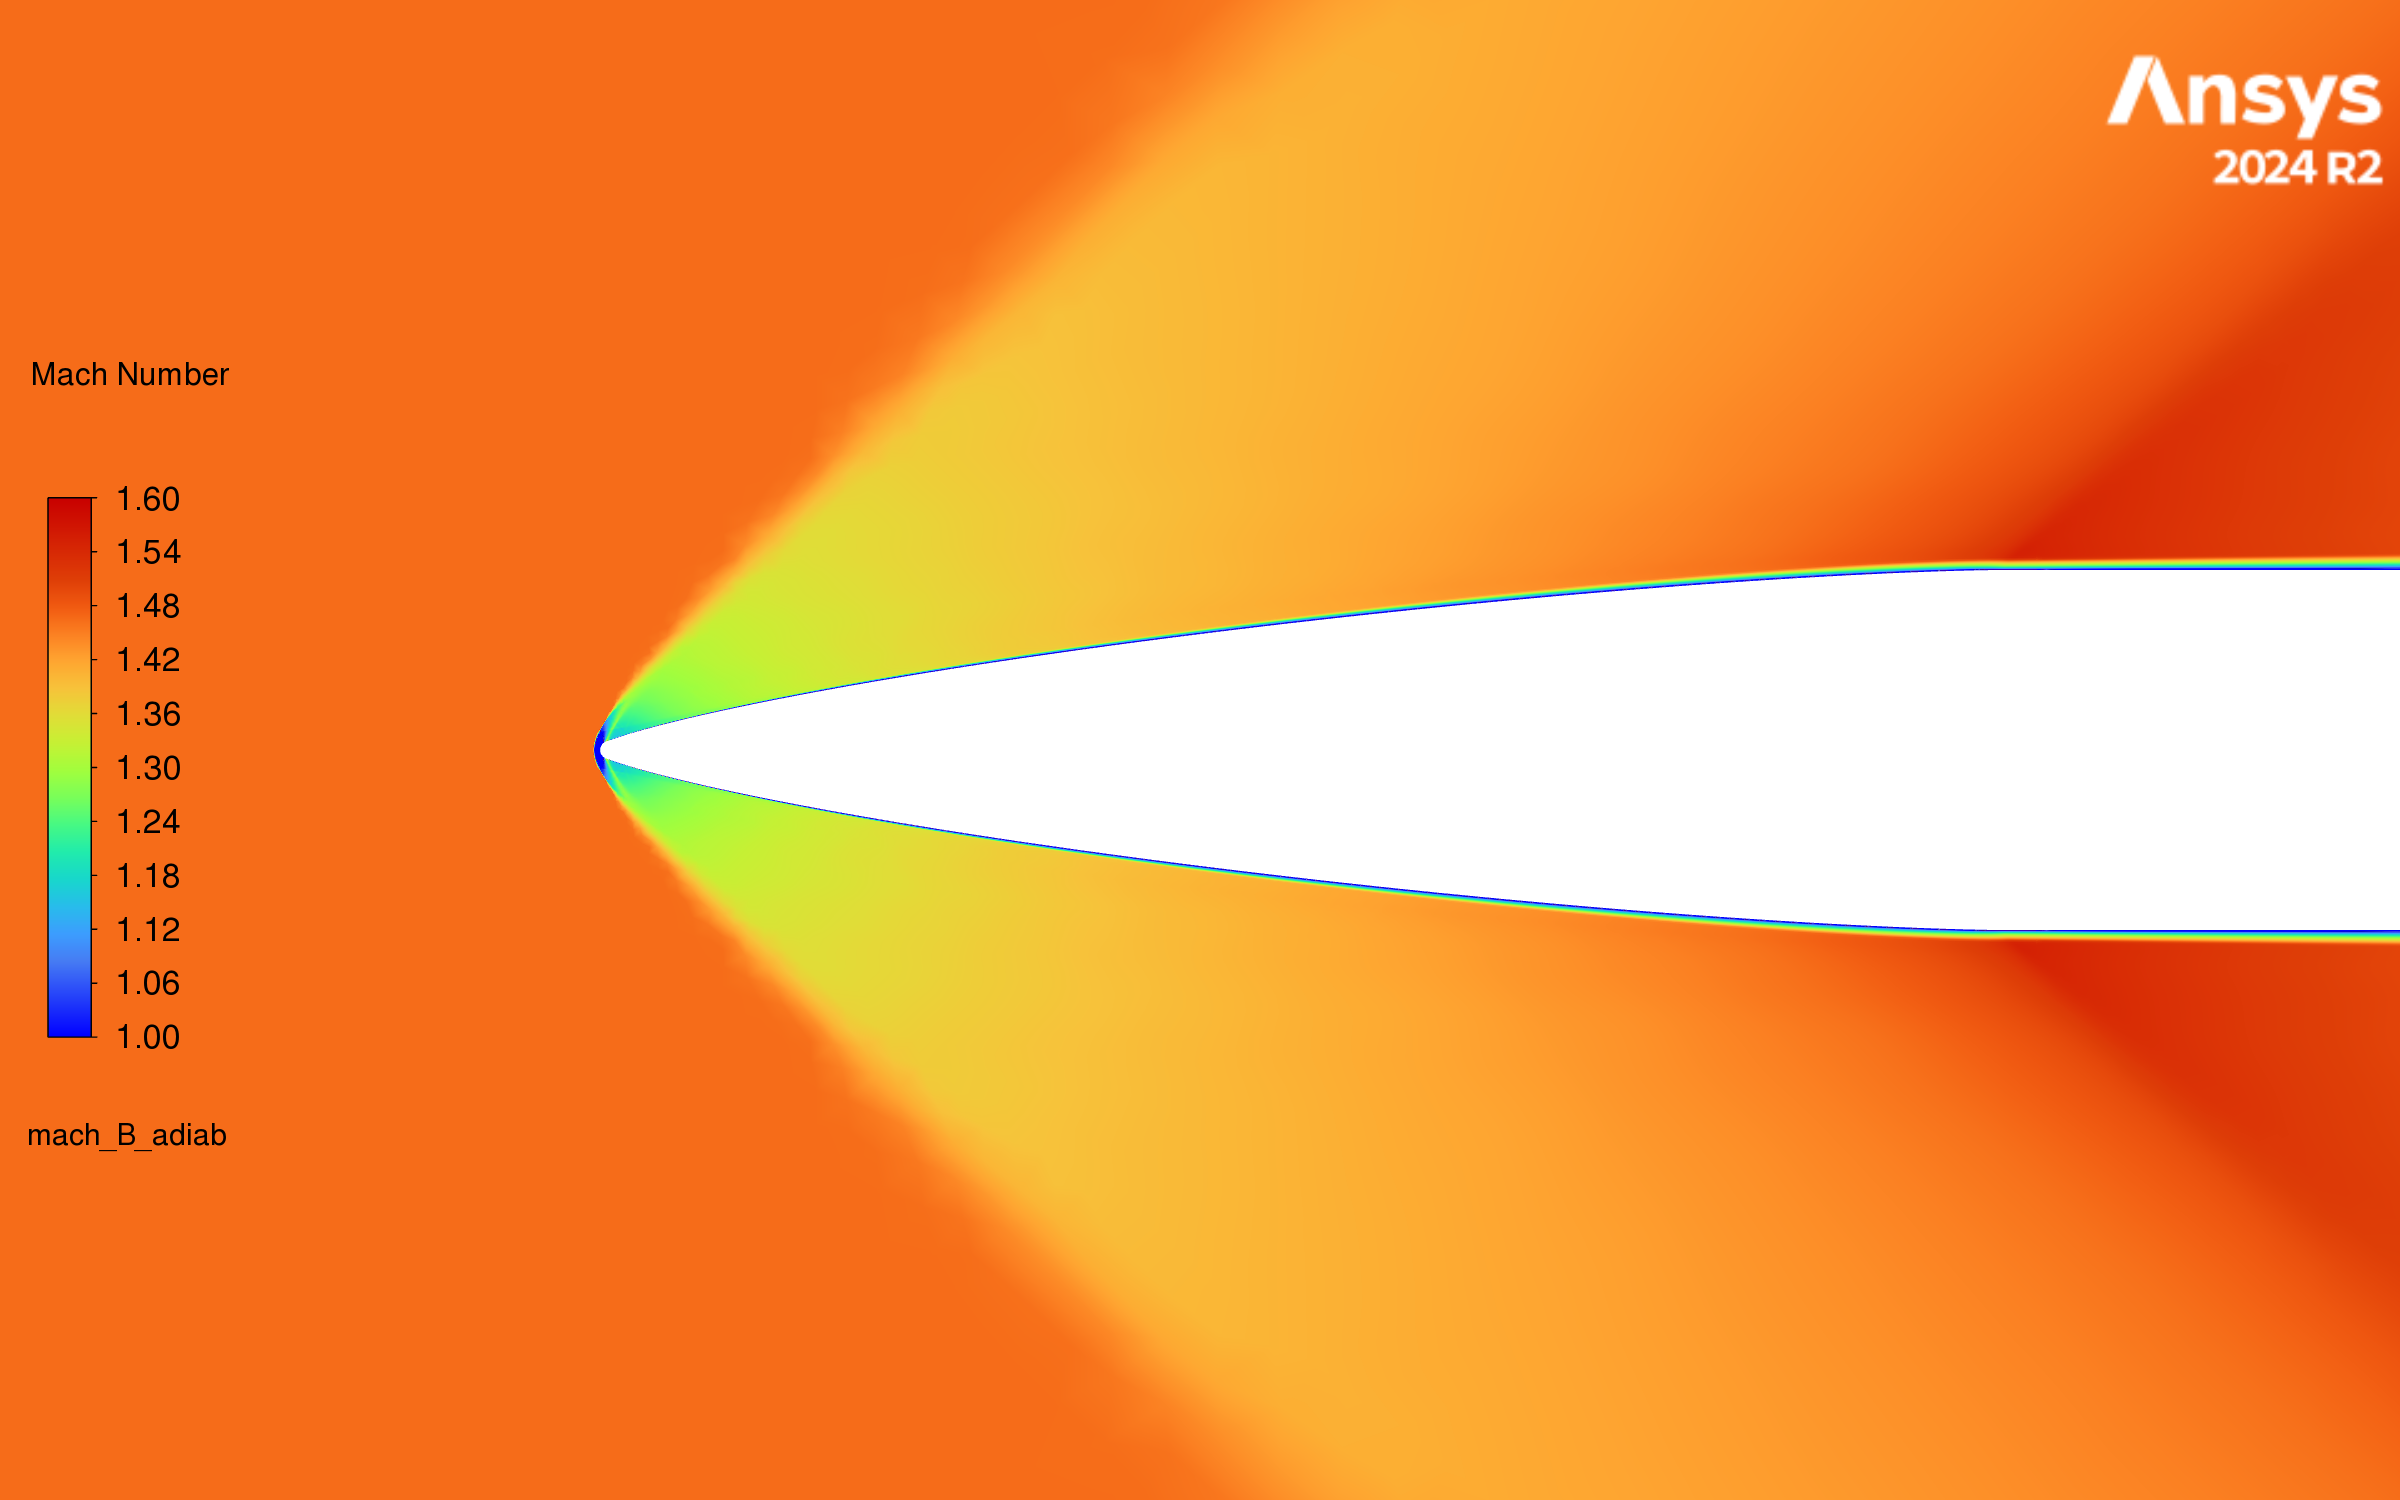
\includegraphics[width=\linewidth]{fluent_mach_B_adiab}
\caption{Design B.}
\end{subfigure}
\caption{Mach number around the nose at burnout (Fluent). Yellow and green: the air slowed down by the bow
shock and the front of the nose.}
\label{fig:mach}
\end{figure}

\begin{figure}[H]
\centering
\begin{subfigure}[t]{0.49\linewidth}
\centering
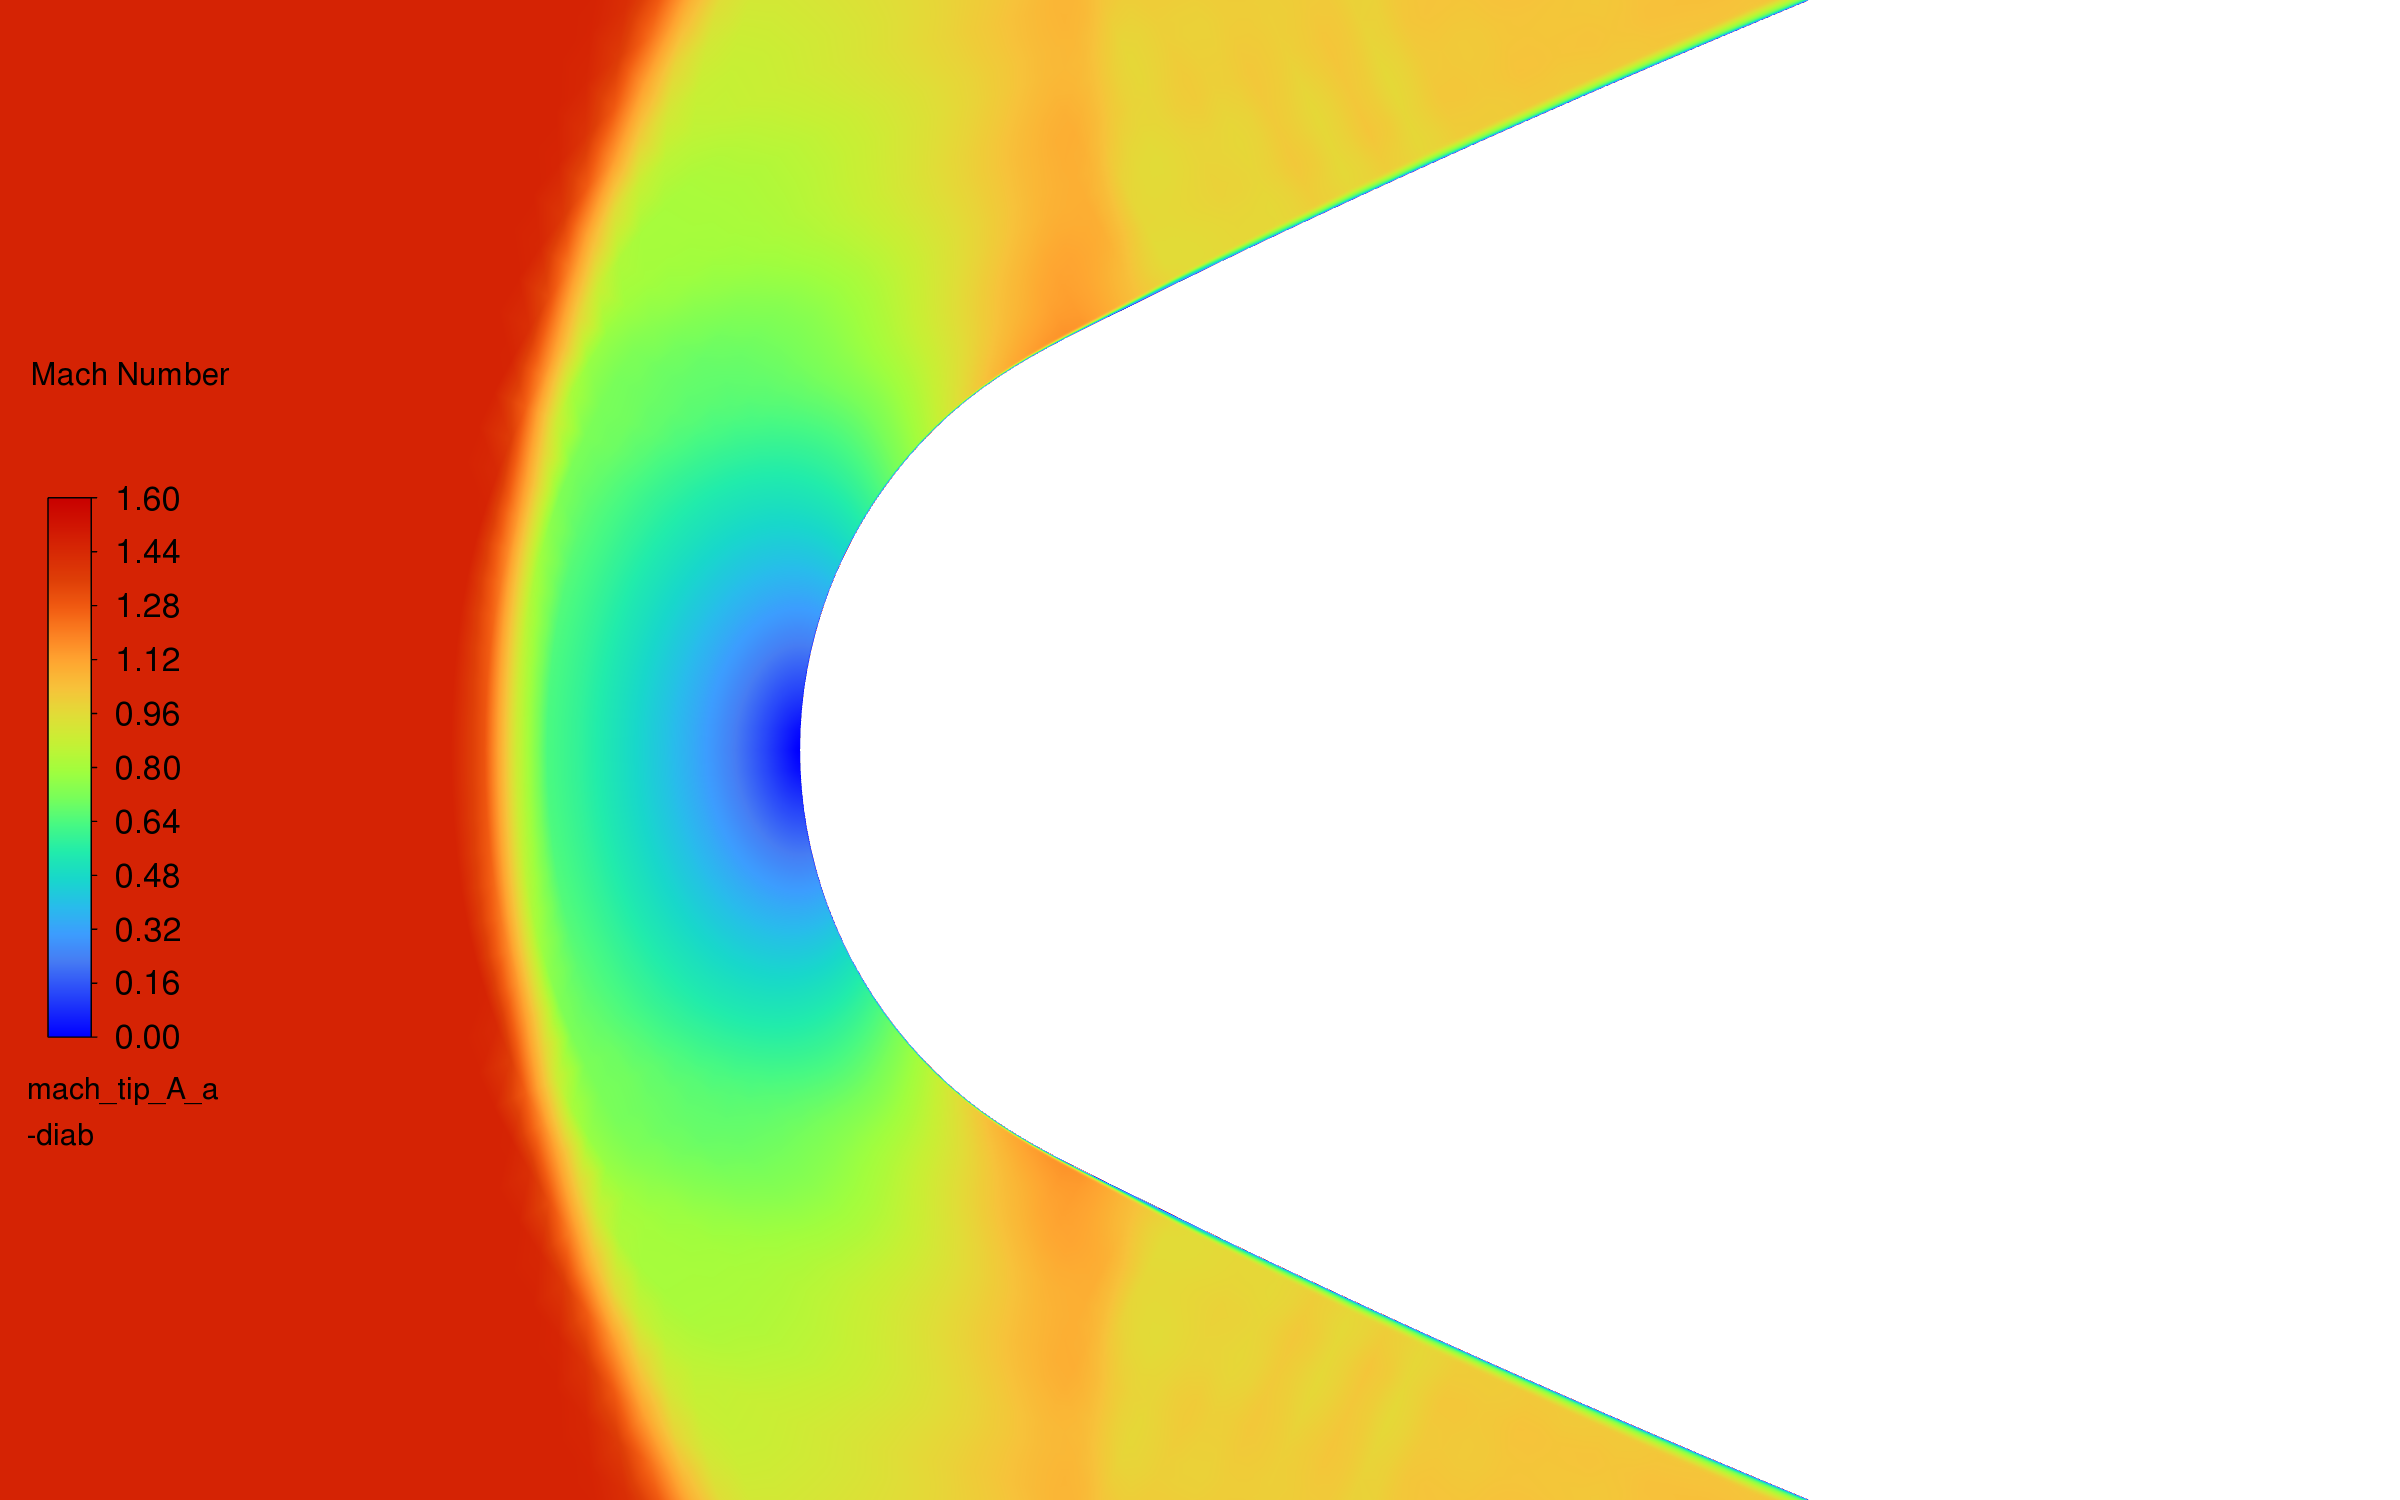
\includegraphics[width=\linewidth]{fluent_mach_tip_A_adiab}
\caption{Design A.}
\end{subfigure}\hfill
\begin{subfigure}[t]{0.49\linewidth}
\centering
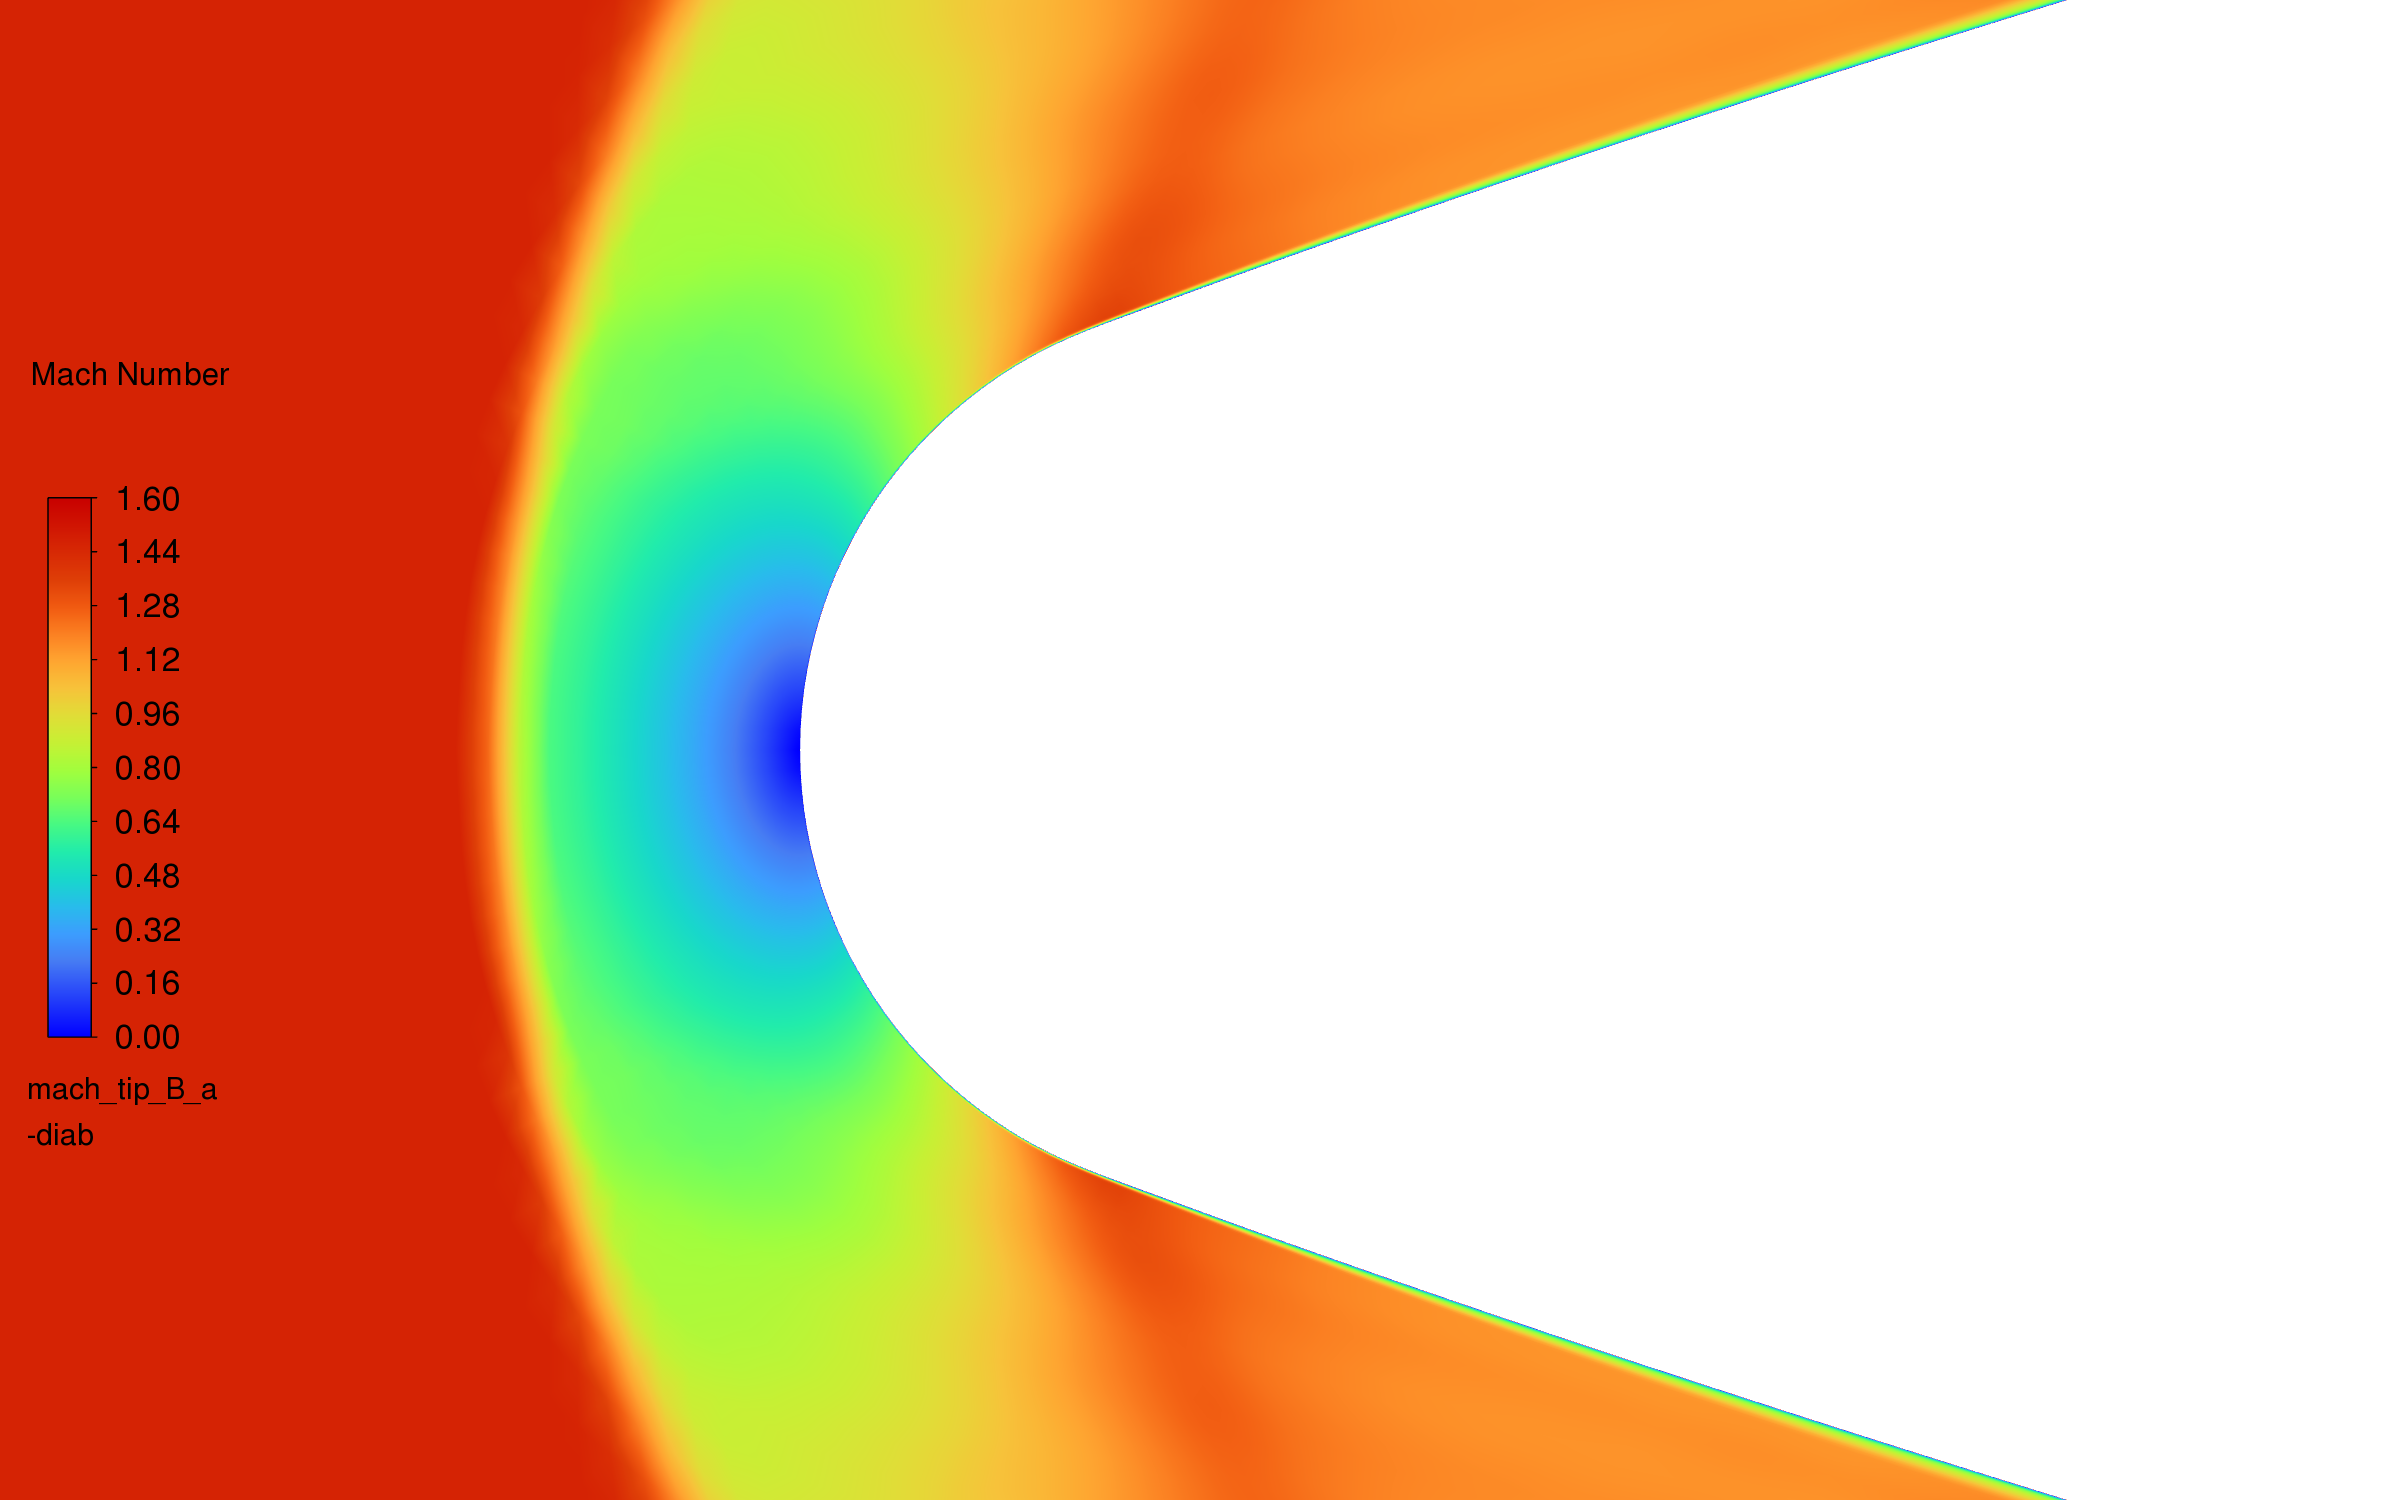
\includegraphics[width=\linewidth]{fluent_mach_tip_B_adiab}
\caption{Design B.}
\end{subfigure}
\caption{Mach number around the tip at burnout (Fluent). The bow shock stands just ahead of the rounded
tip, with a small subsonic region behind it.}
\label{fig:machtip}
\end{figure}

\begin{figure}[H]
\centering
\begin{subfigure}[t]{0.49\linewidth}
\centering
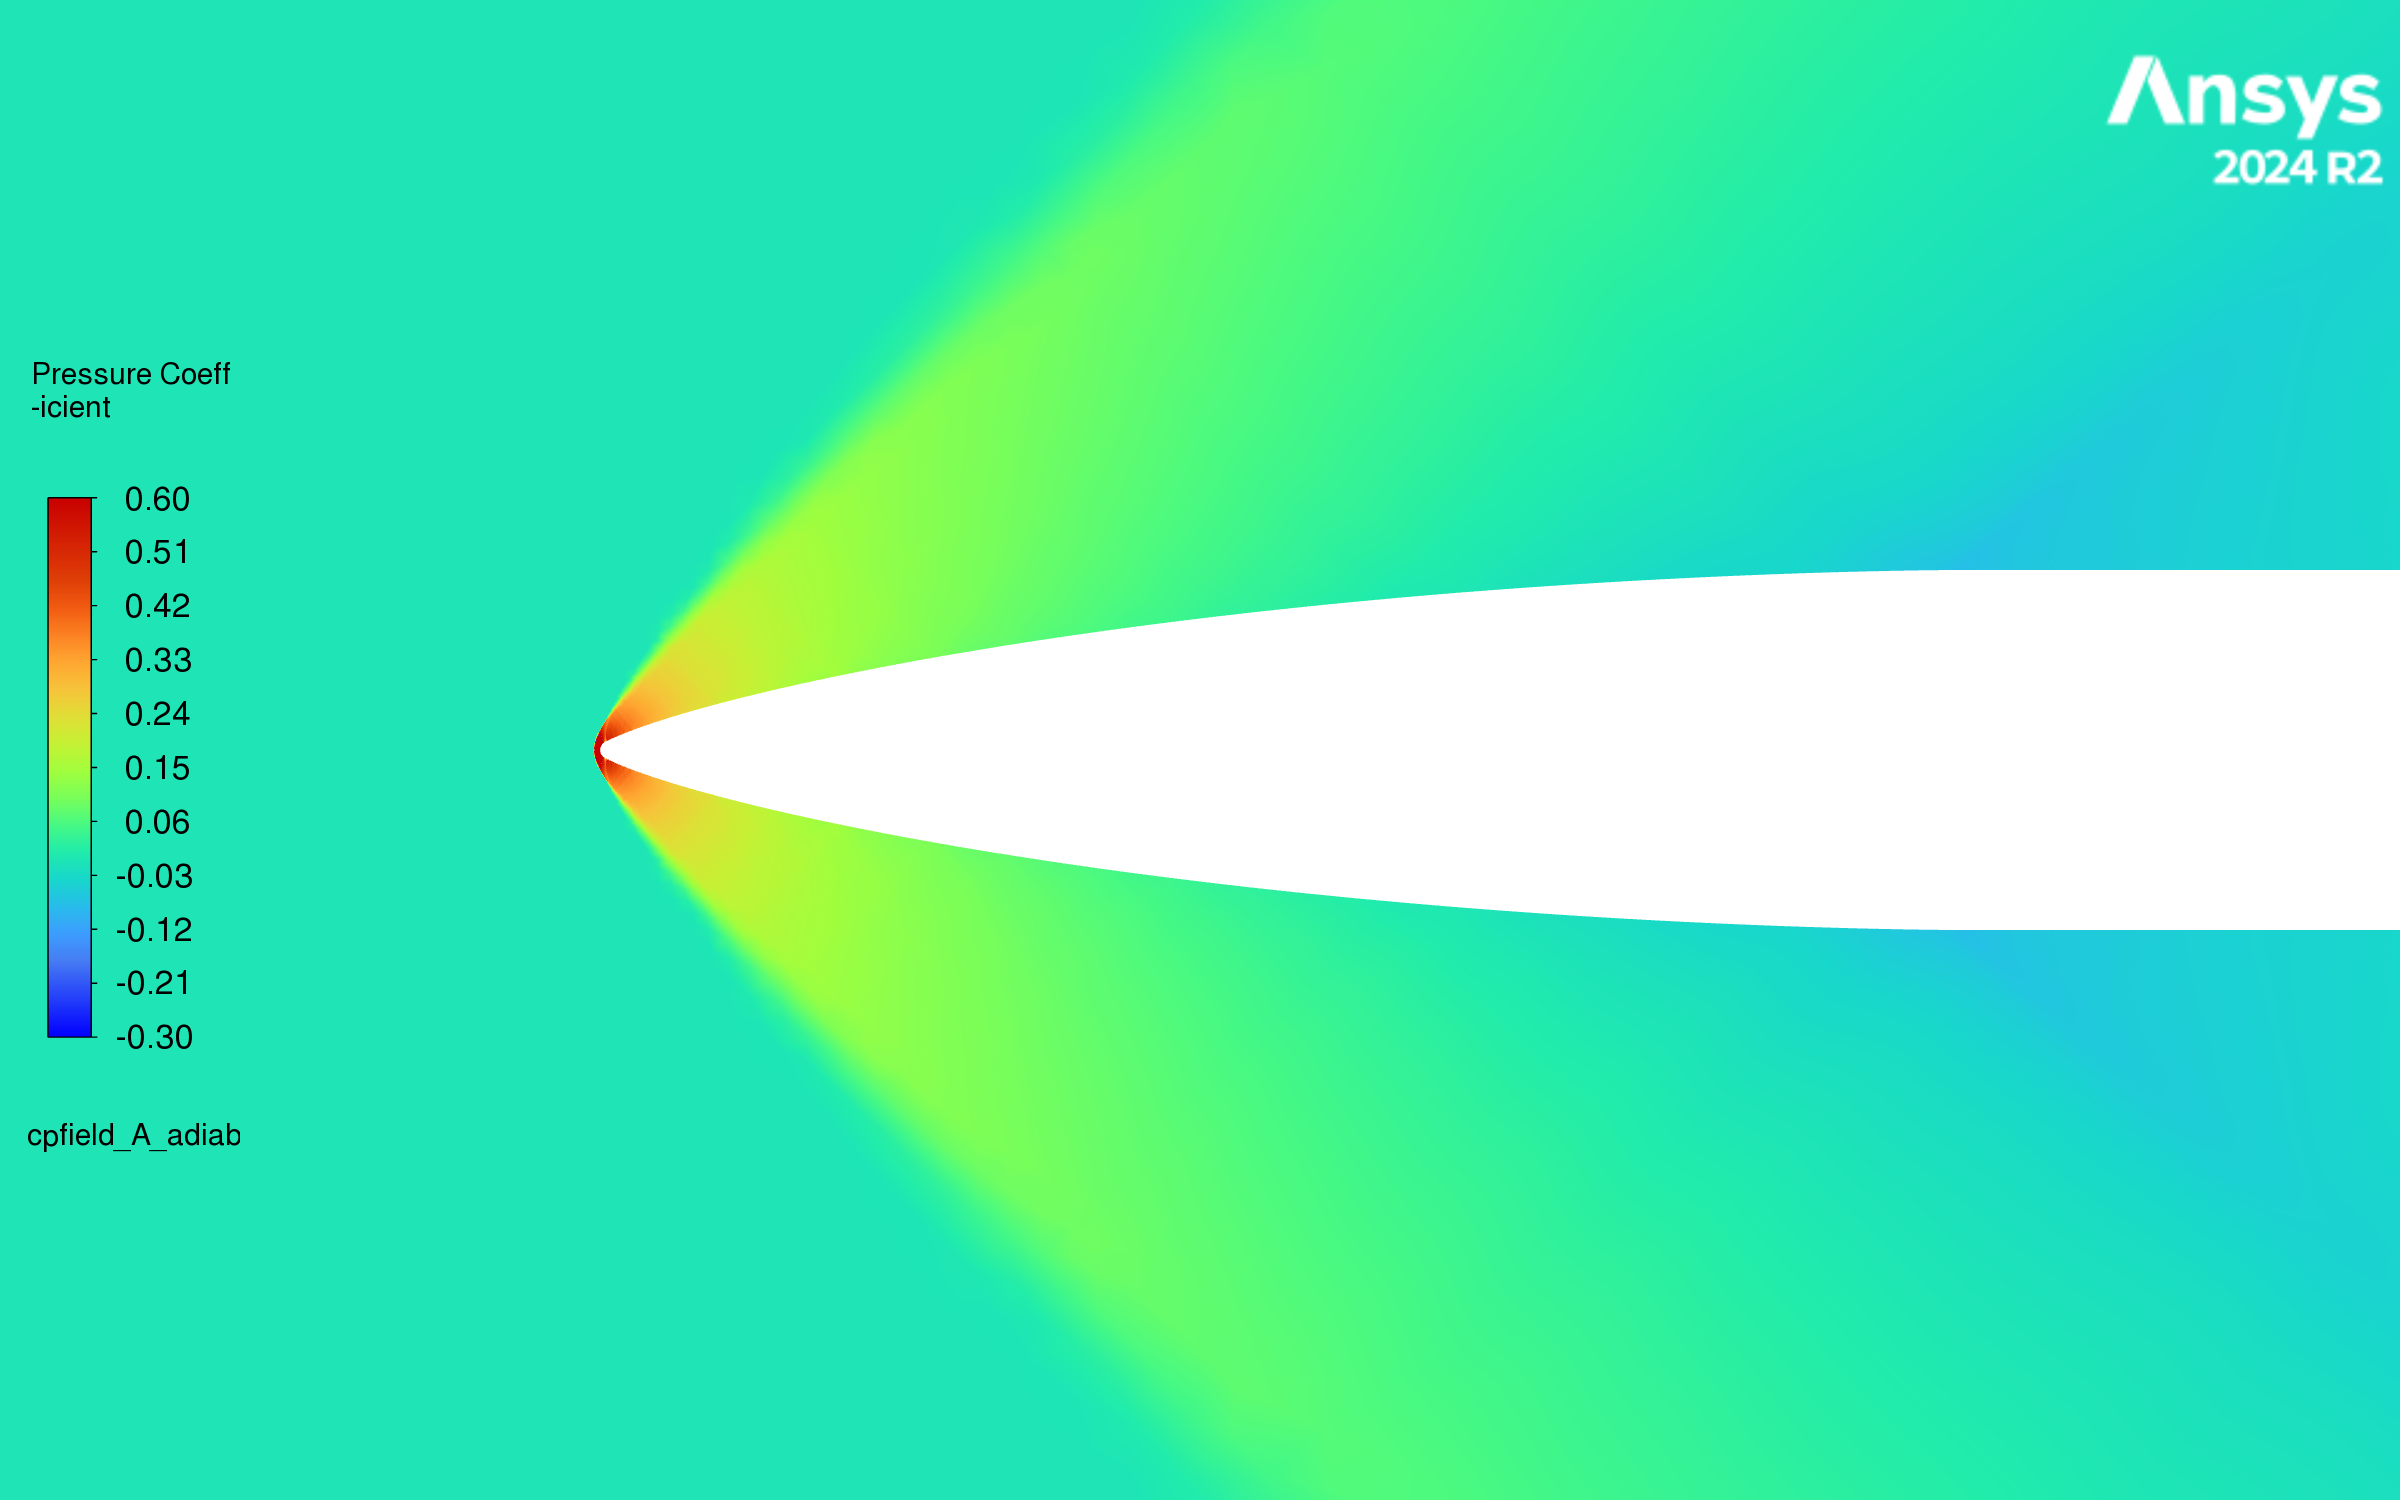
\includegraphics[width=\linewidth]{fluent_cpfield_A_adiab}
\caption{Design A.}
\end{subfigure}\hfill
\begin{subfigure}[t]{0.49\linewidth}
\centering
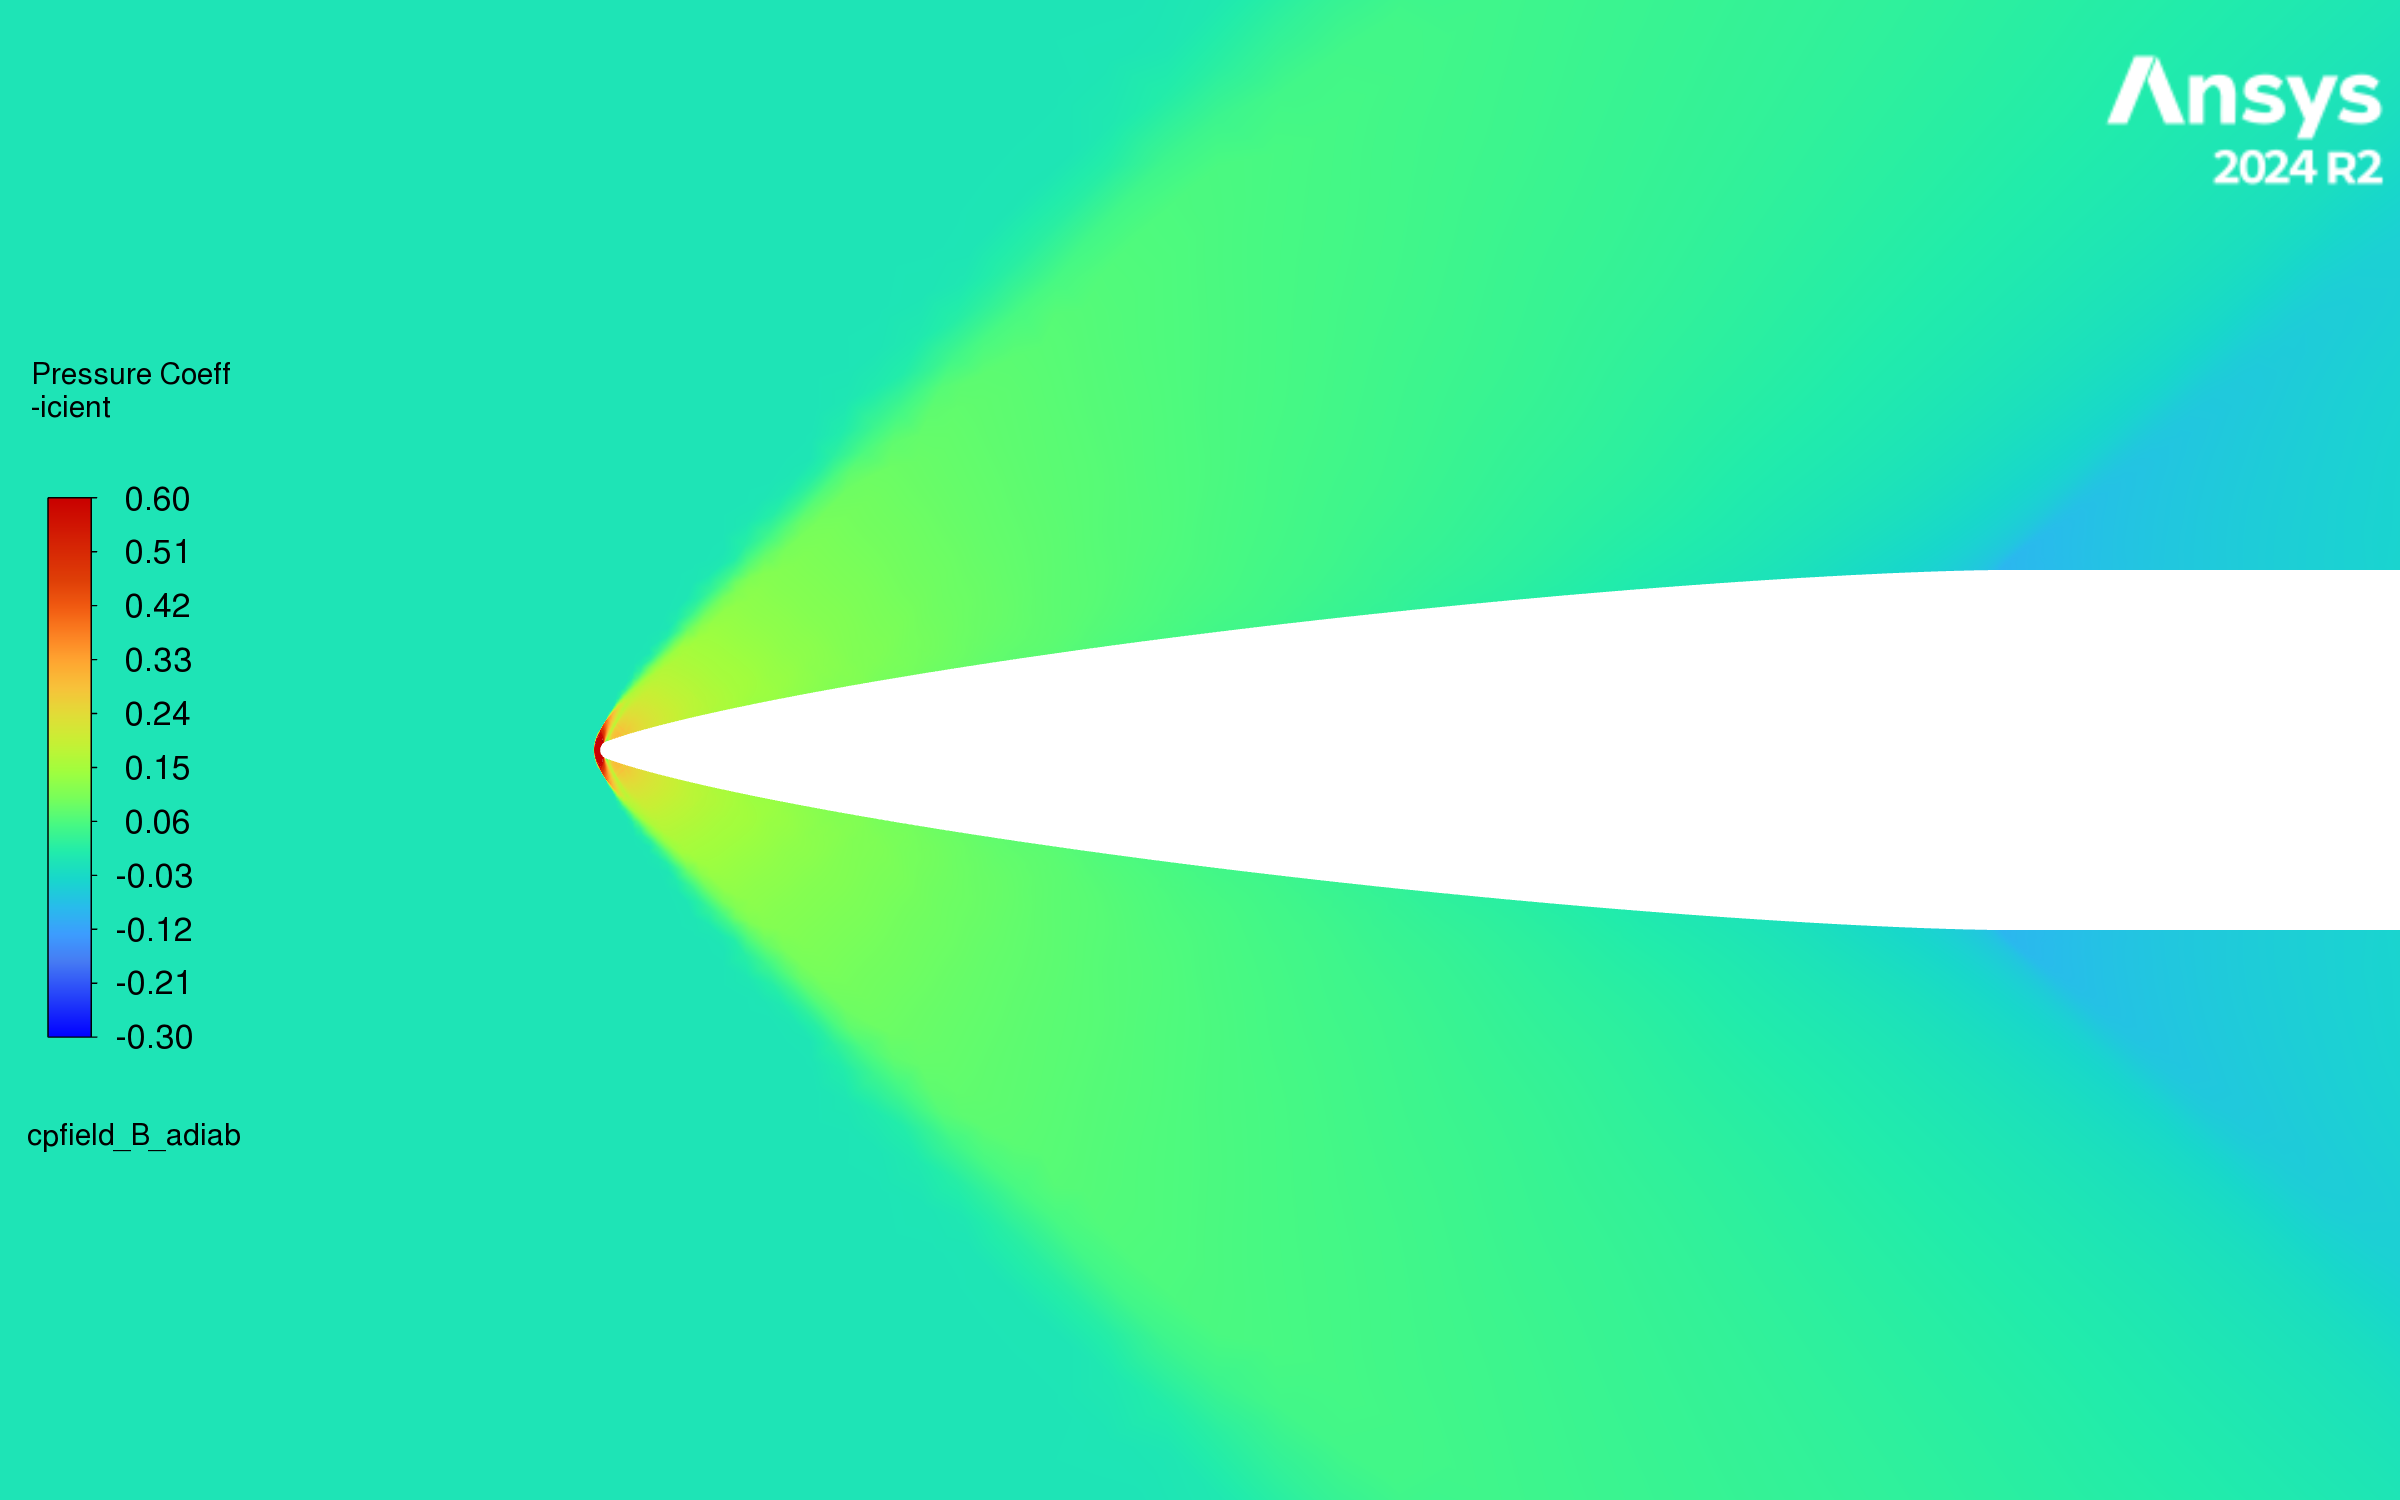
\includegraphics[width=\linewidth]{fluent_cpfield_B_adiab}
\caption{Design B.}
\end{subfigure}
\caption{Pressure coefficient around the nose at burnout (Fluent), $C_p = (p - p_\infty)/q$. Warm colours:
pressure above the outside pressure, which pushes the nose back.}
\label{fig:cpfield}
\end{figure}

\begin{figure}[H]
\centering
\begin{subfigure}[t]{\linewidth}
\centering
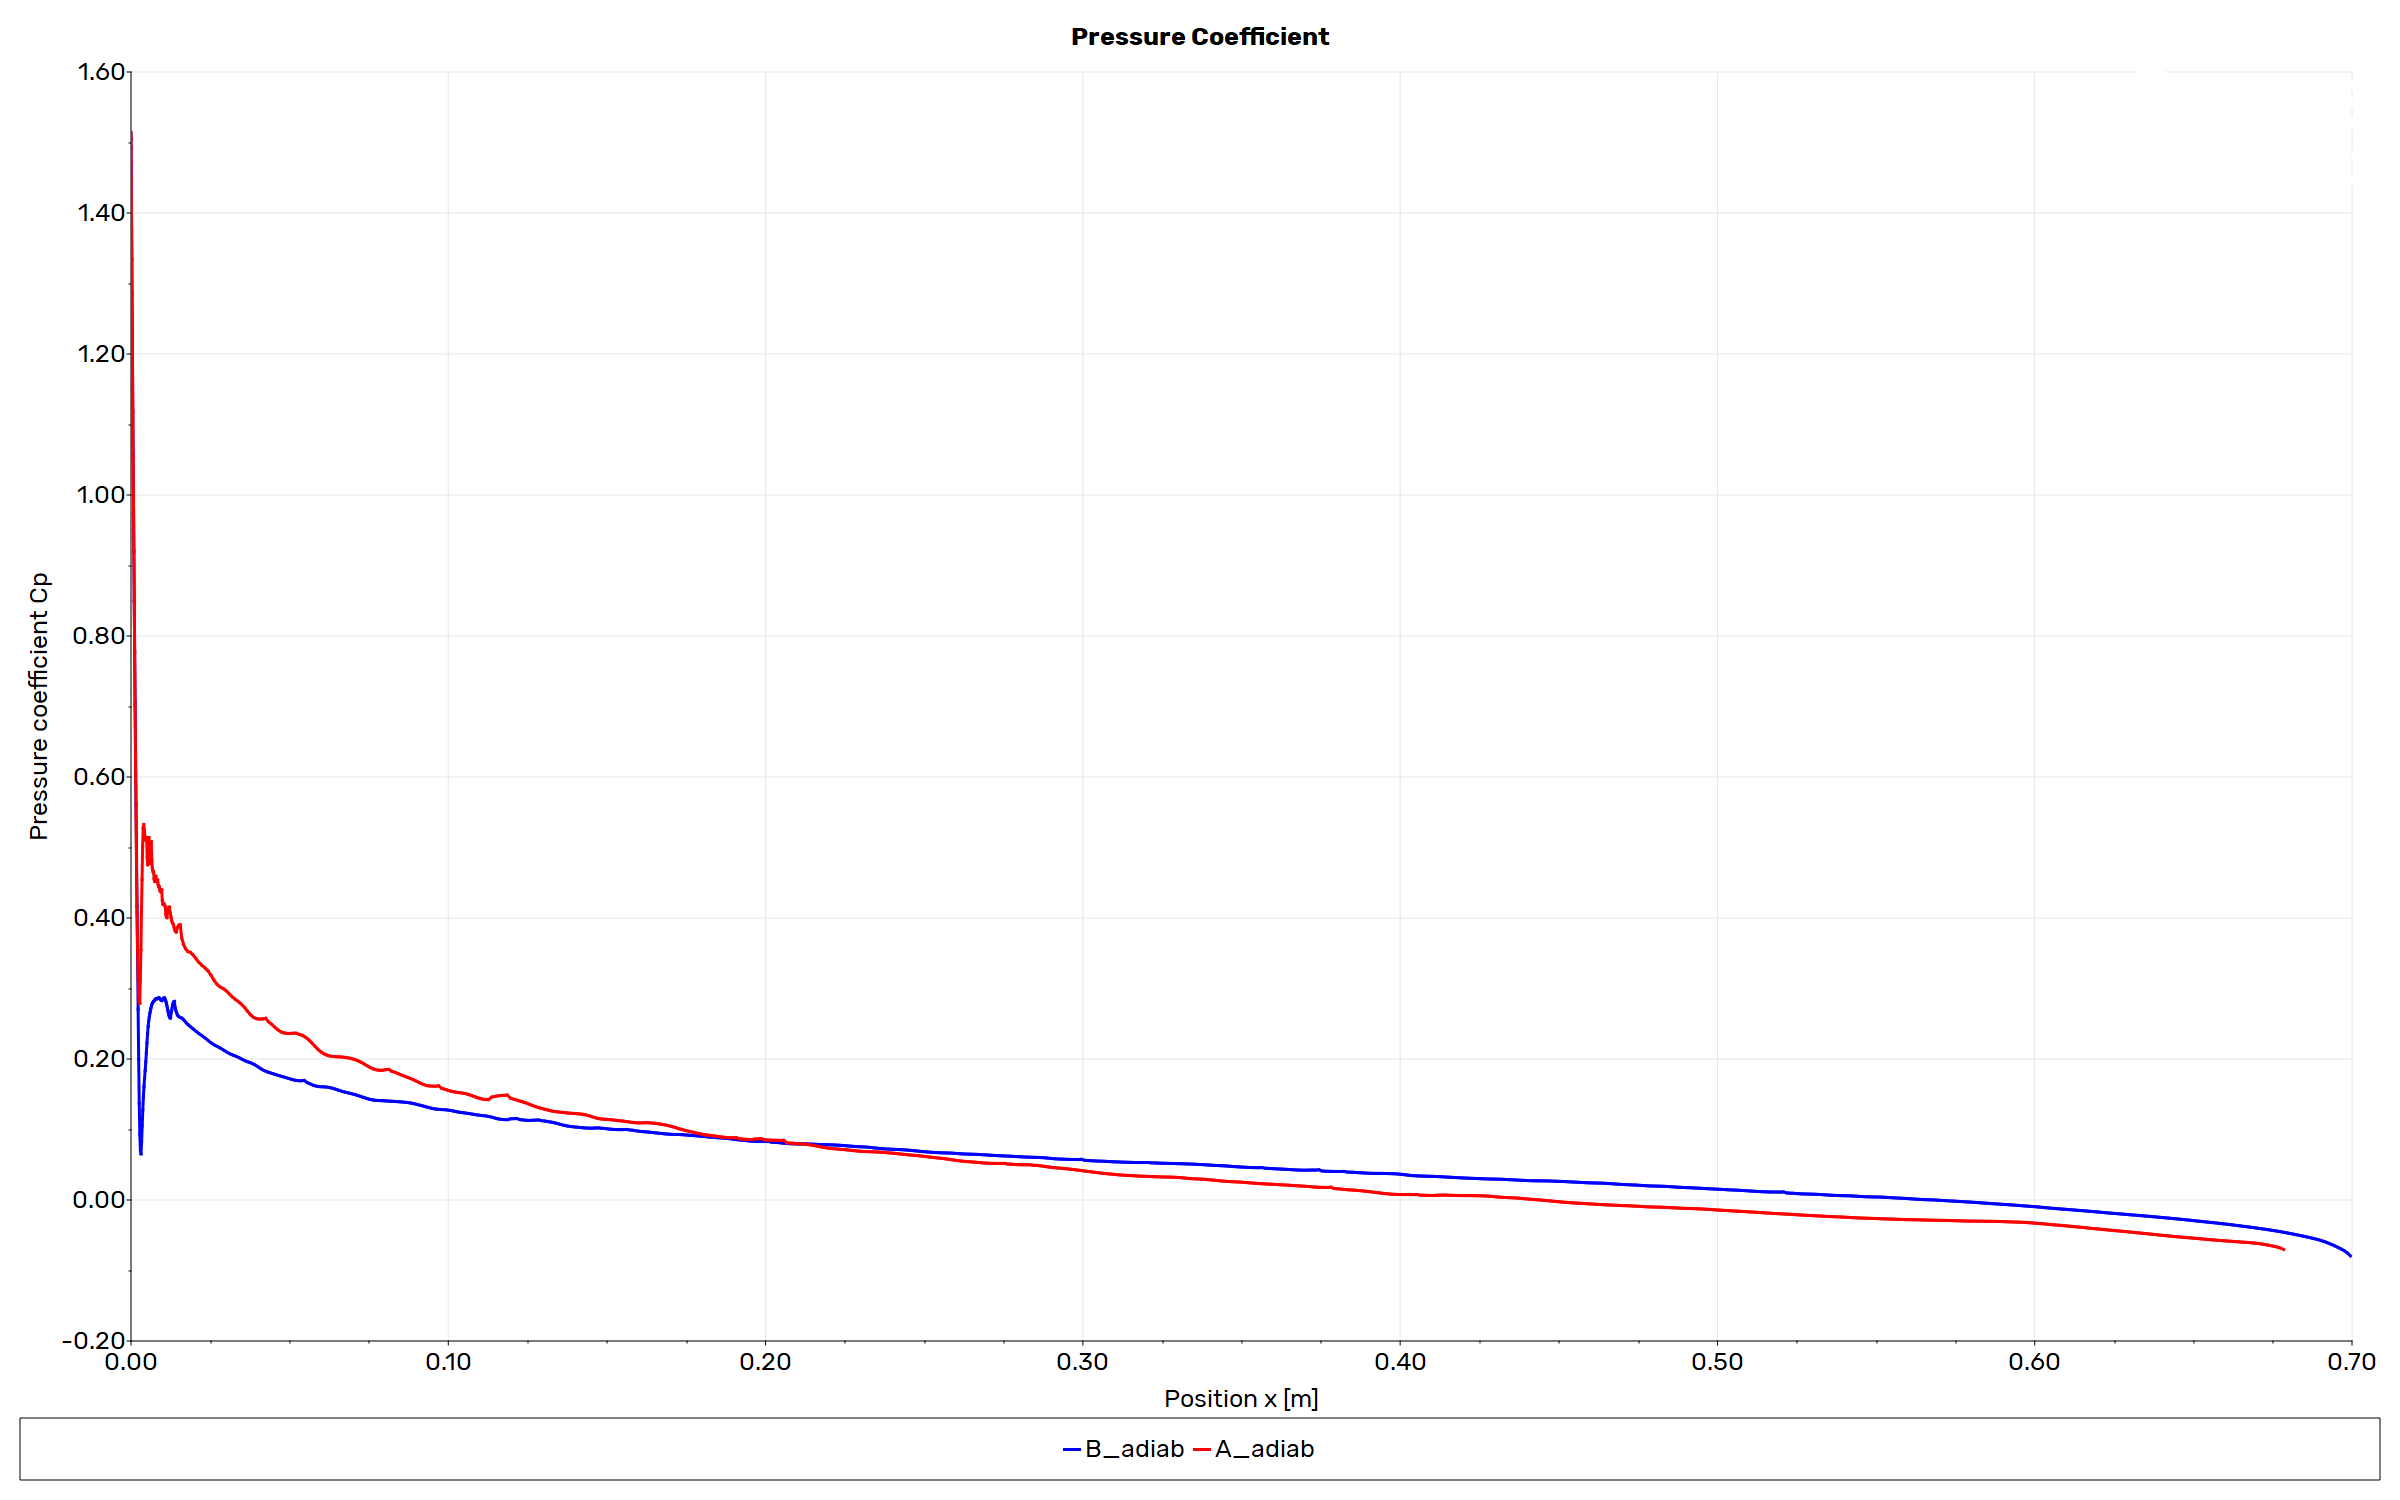
\includegraphics[width=\linewidth]{fluent_cp_AB_adiab}
\caption{Burnout, $M = \val{pt-M147-M}$.}
\end{subfigure}

\medskip
\begin{subfigure}[t]{\linewidth}
\centering
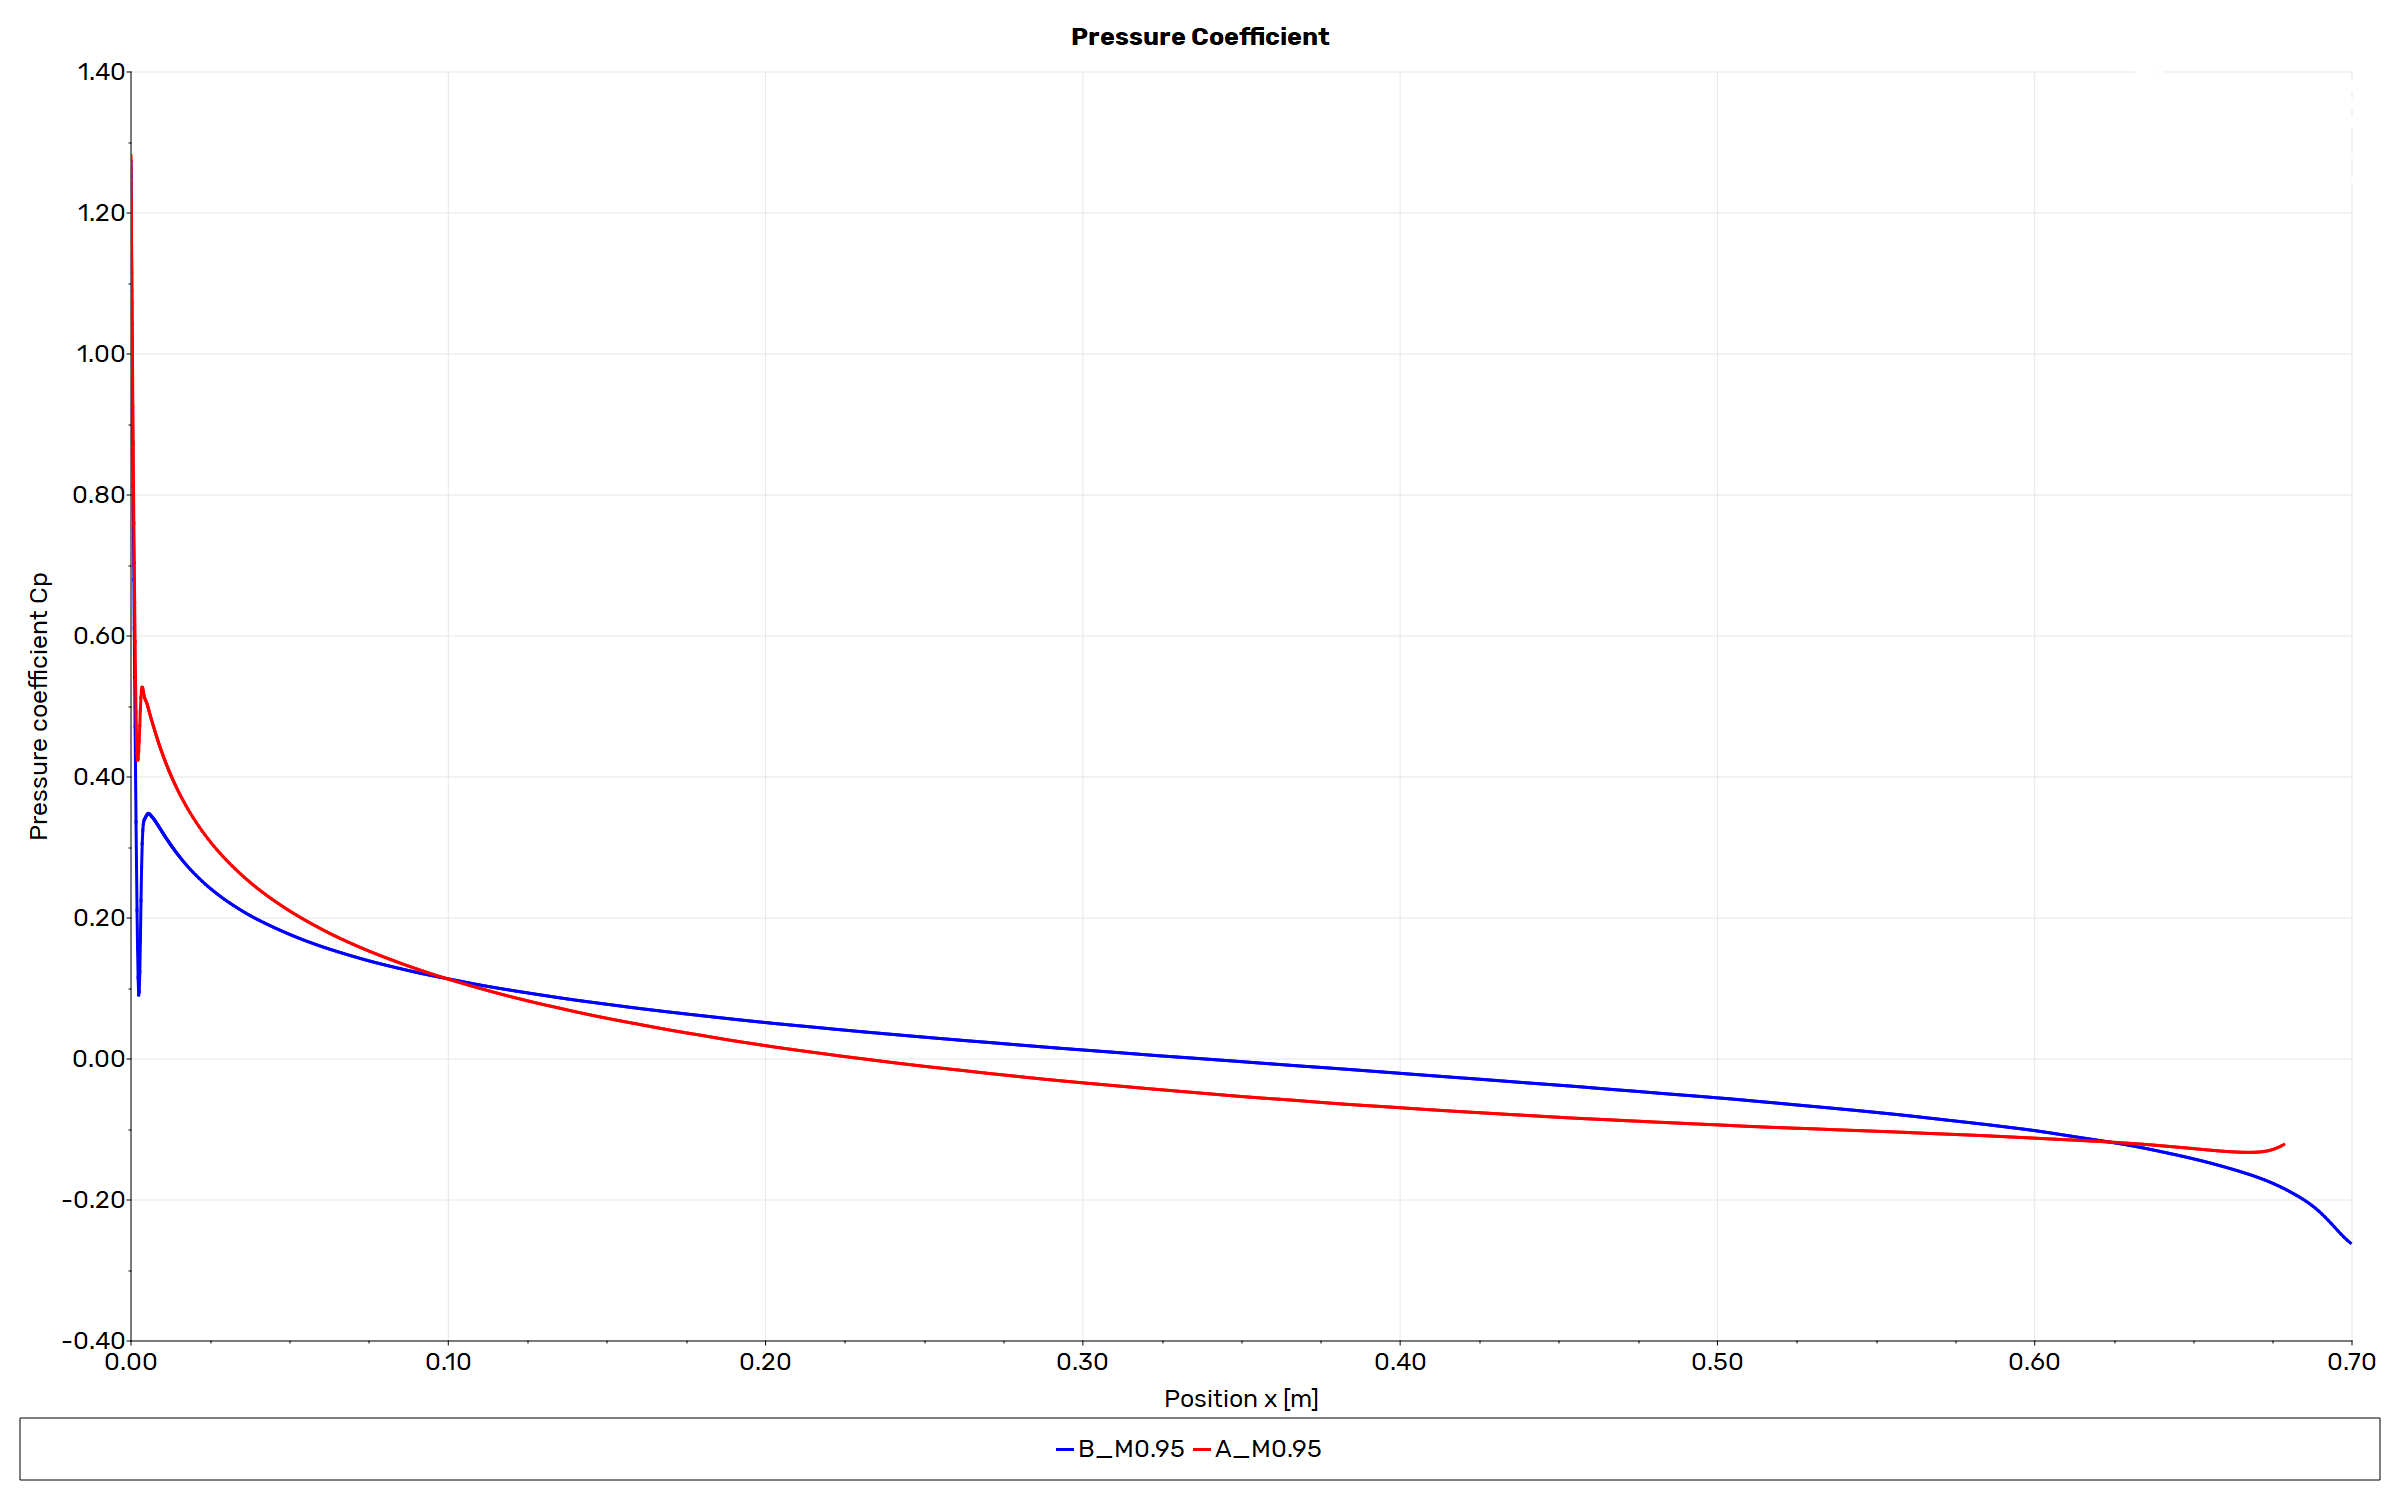
\includegraphics[width=\linewidth]{fluent_cp_AB_M0.95}
\caption{Transonic, $M = 0.95$.}
\end{subfigure}
\caption{Pressure coefficient along the wall, design A (red) and B (blue), Fluent. The $M = 1.20$ run lies
between the two.}
\label{fig:cp}
\end{figure}

\subsection{Below Mach 1: same drag}

At $M = 0.95$ no bow shock forms ahead of the nose (Figure~\ref{fig:mach095}). The pressure drag is only
about 5\,N for both designs (Table~\ref{tab:forces}), so the drag is almost all skin friction. The friction
along the wall is nearly the same for both noses (Figure~\ref{fig:cf}), so their drag is the same.

\begin{figure}[H]
\centering
\begin{subfigure}[t]{0.49\linewidth}
\centering
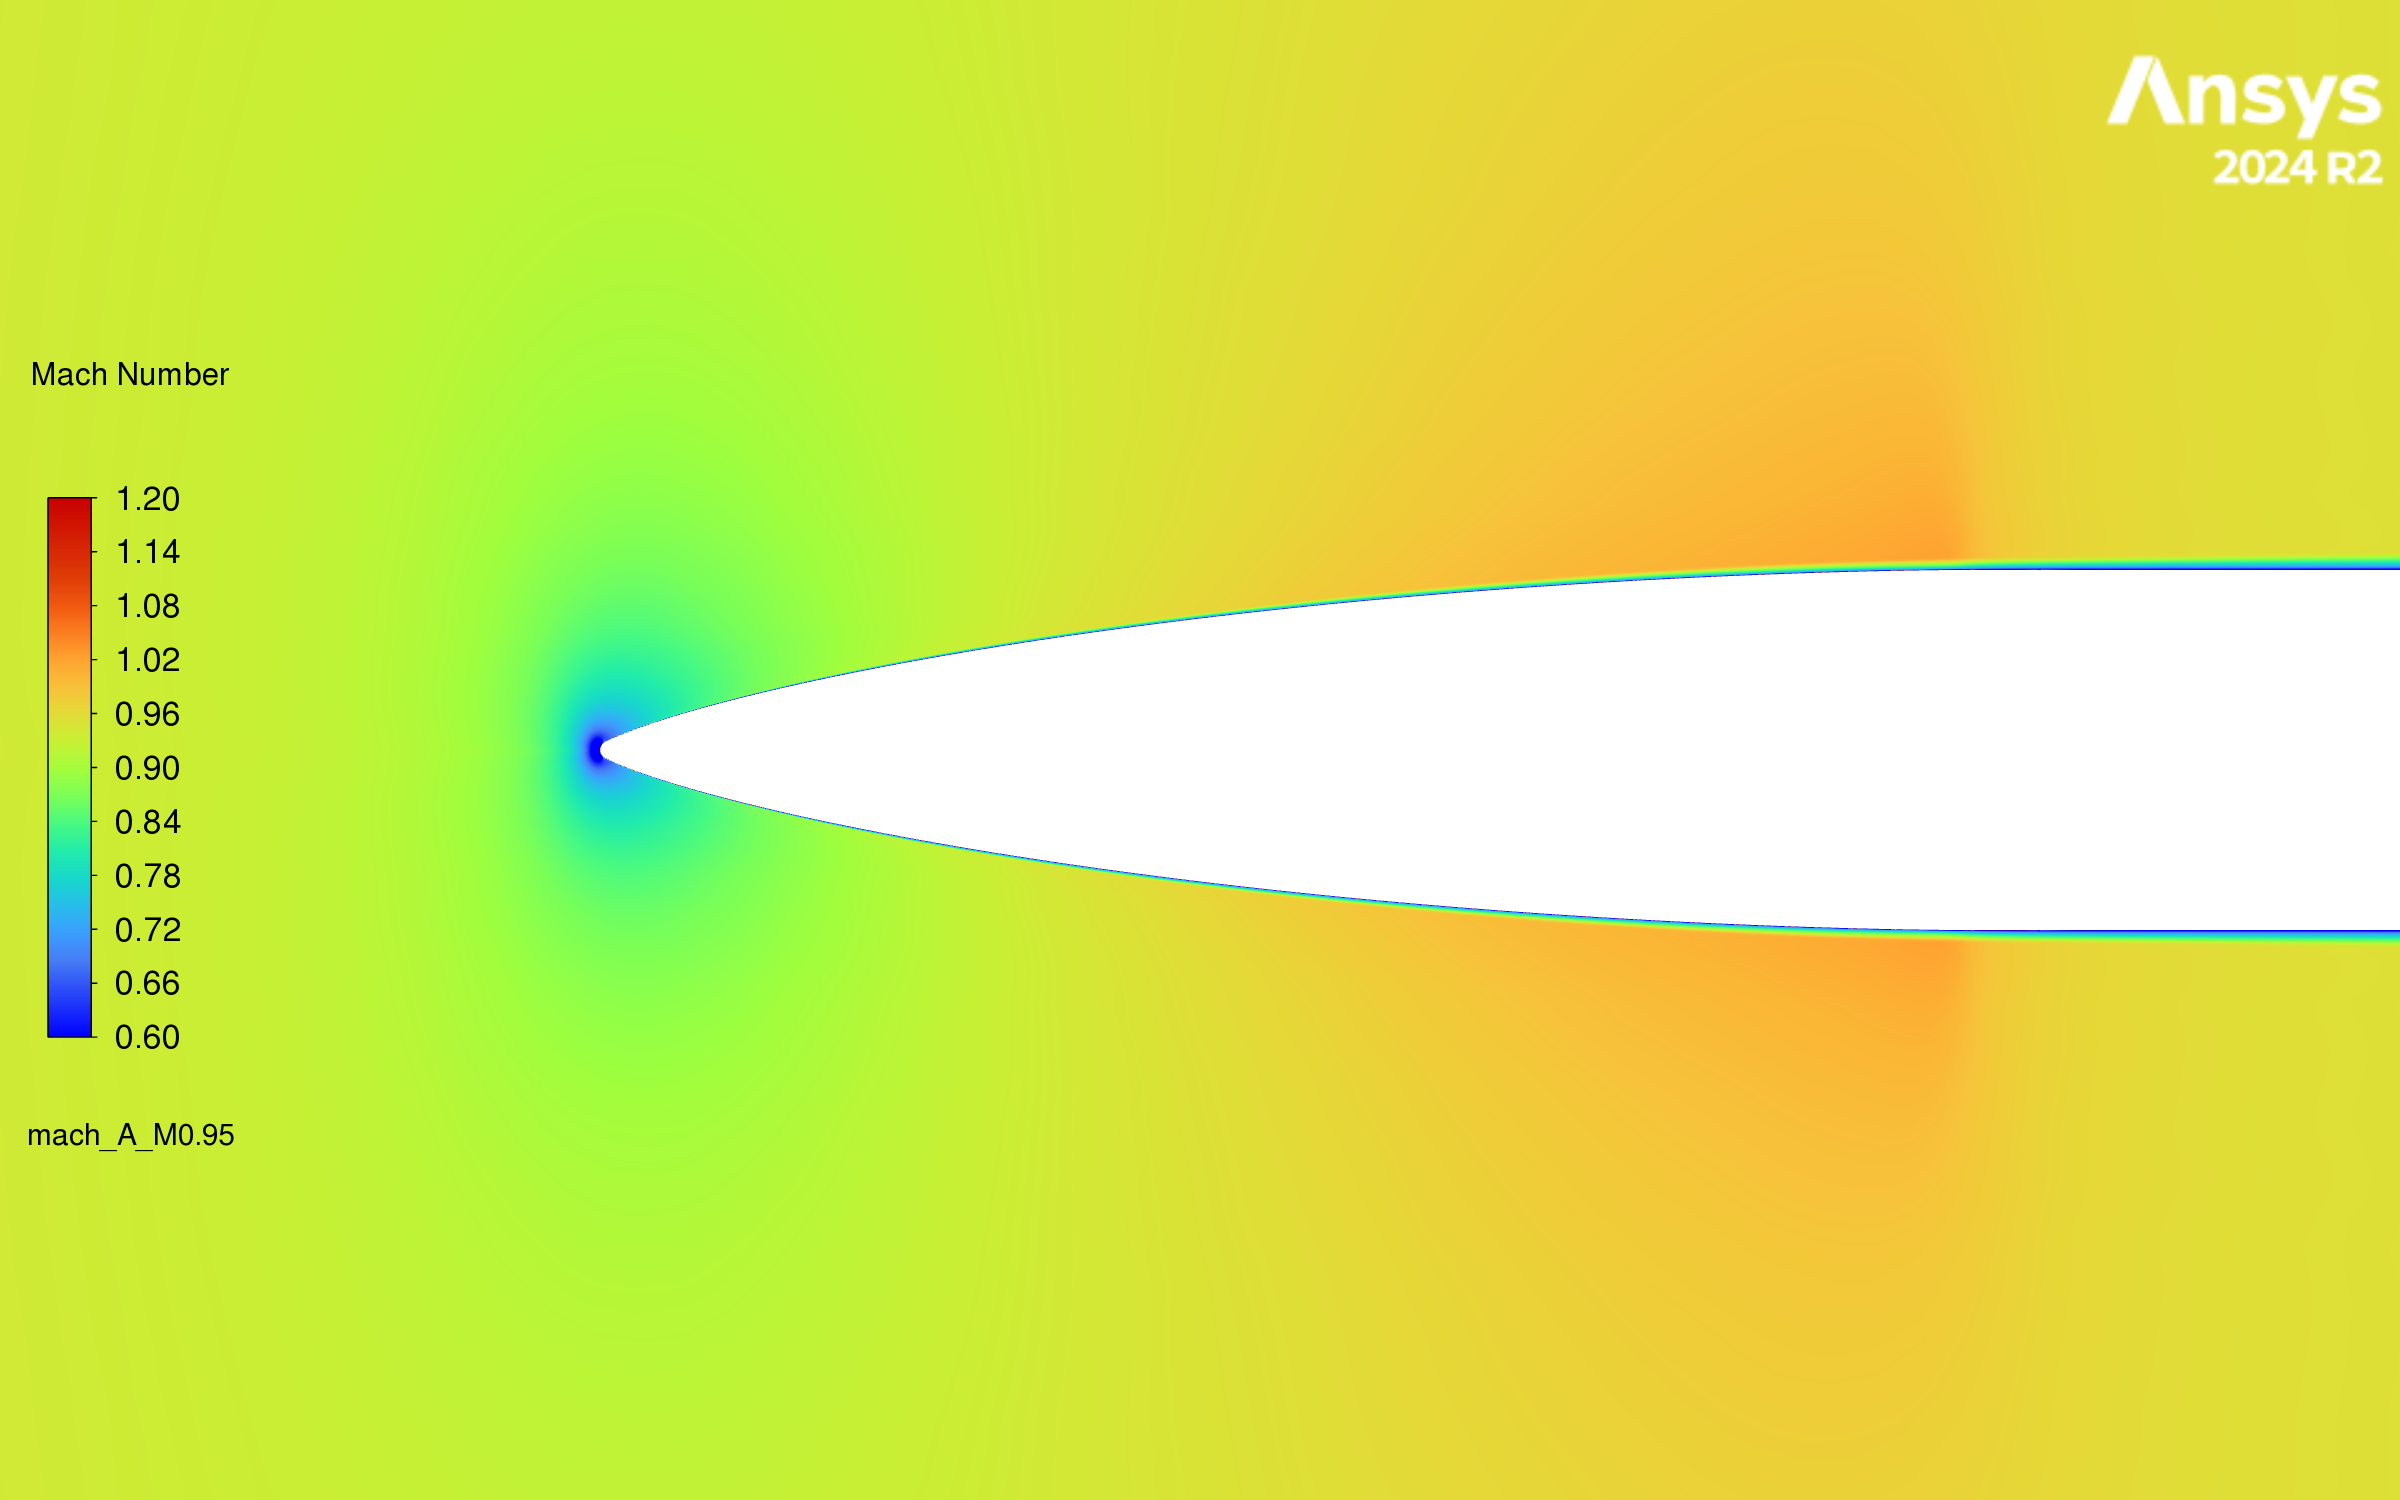
\includegraphics[width=\linewidth]{fluent_mach_A_M0.95}
\caption{Design A.}
\end{subfigure}\hfill
\begin{subfigure}[t]{0.49\linewidth}
\centering
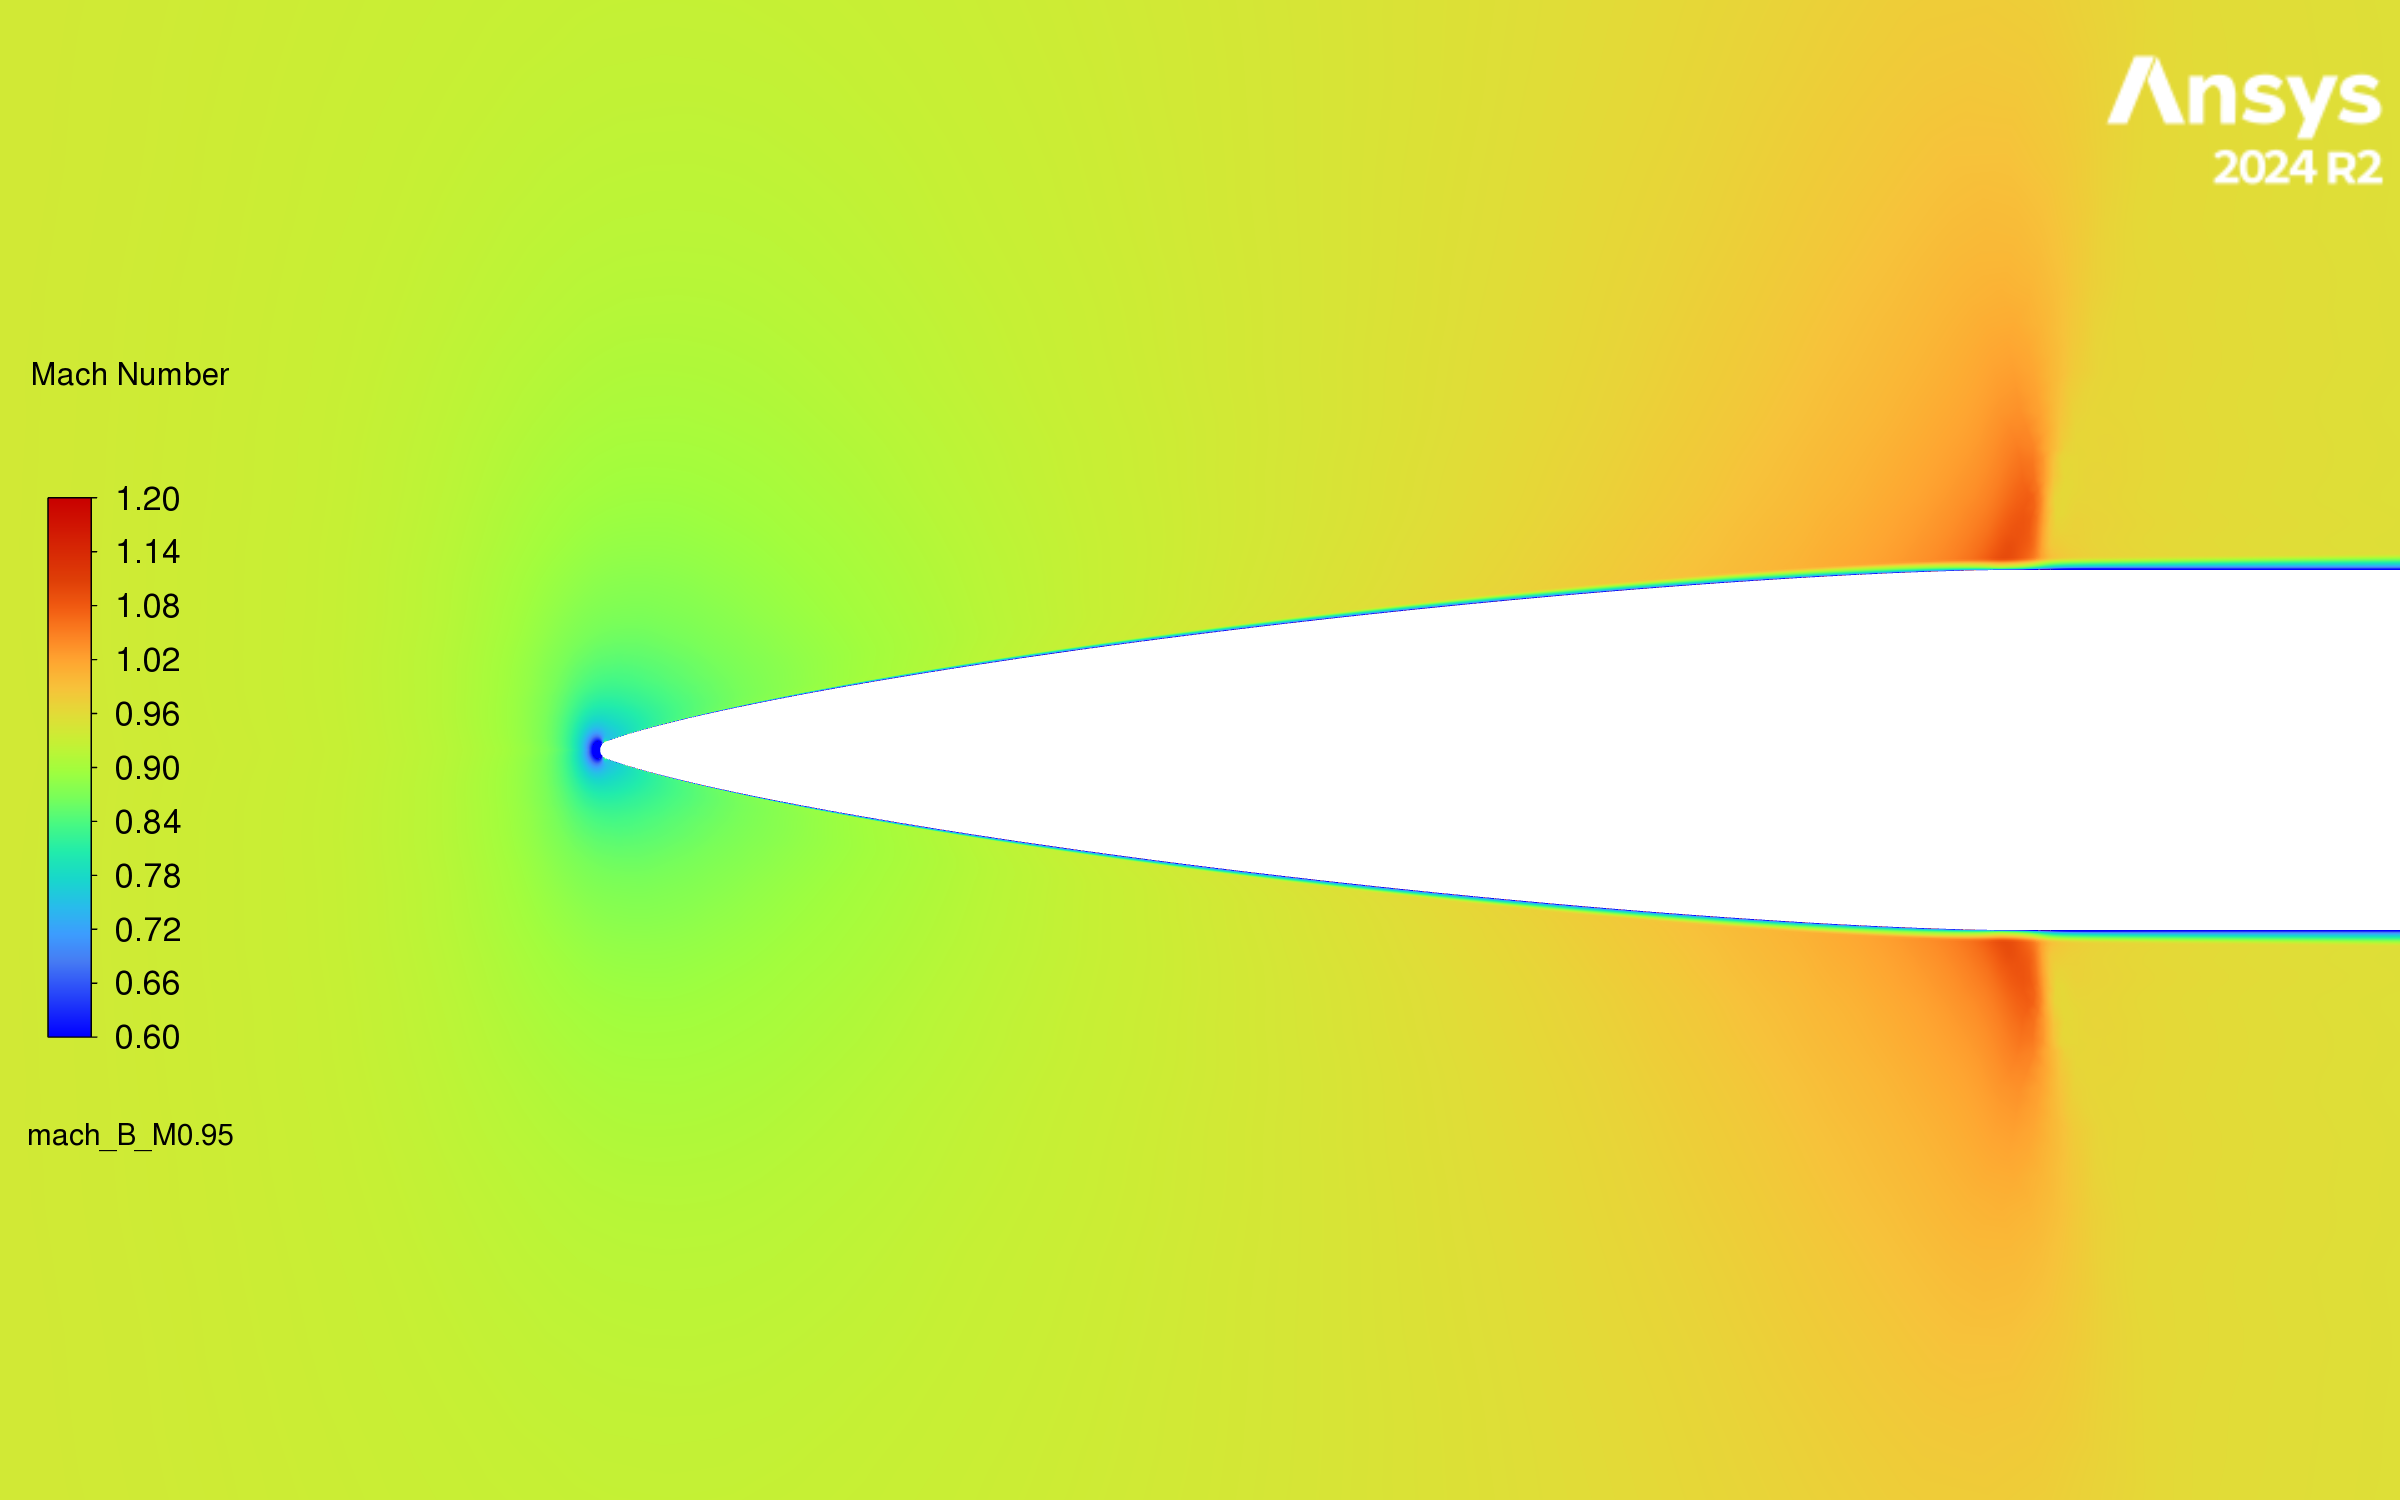
\includegraphics[width=\linewidth]{fluent_mach_B_M0.95}
\caption{Design B.}
\end{subfigure}
\caption{Mach number around the nose at $M = 0.95$ (Fluent). The air speeds up over the shoulder.}
\label{fig:mach095}
\end{figure}

\begin{figure}[H]
\centering
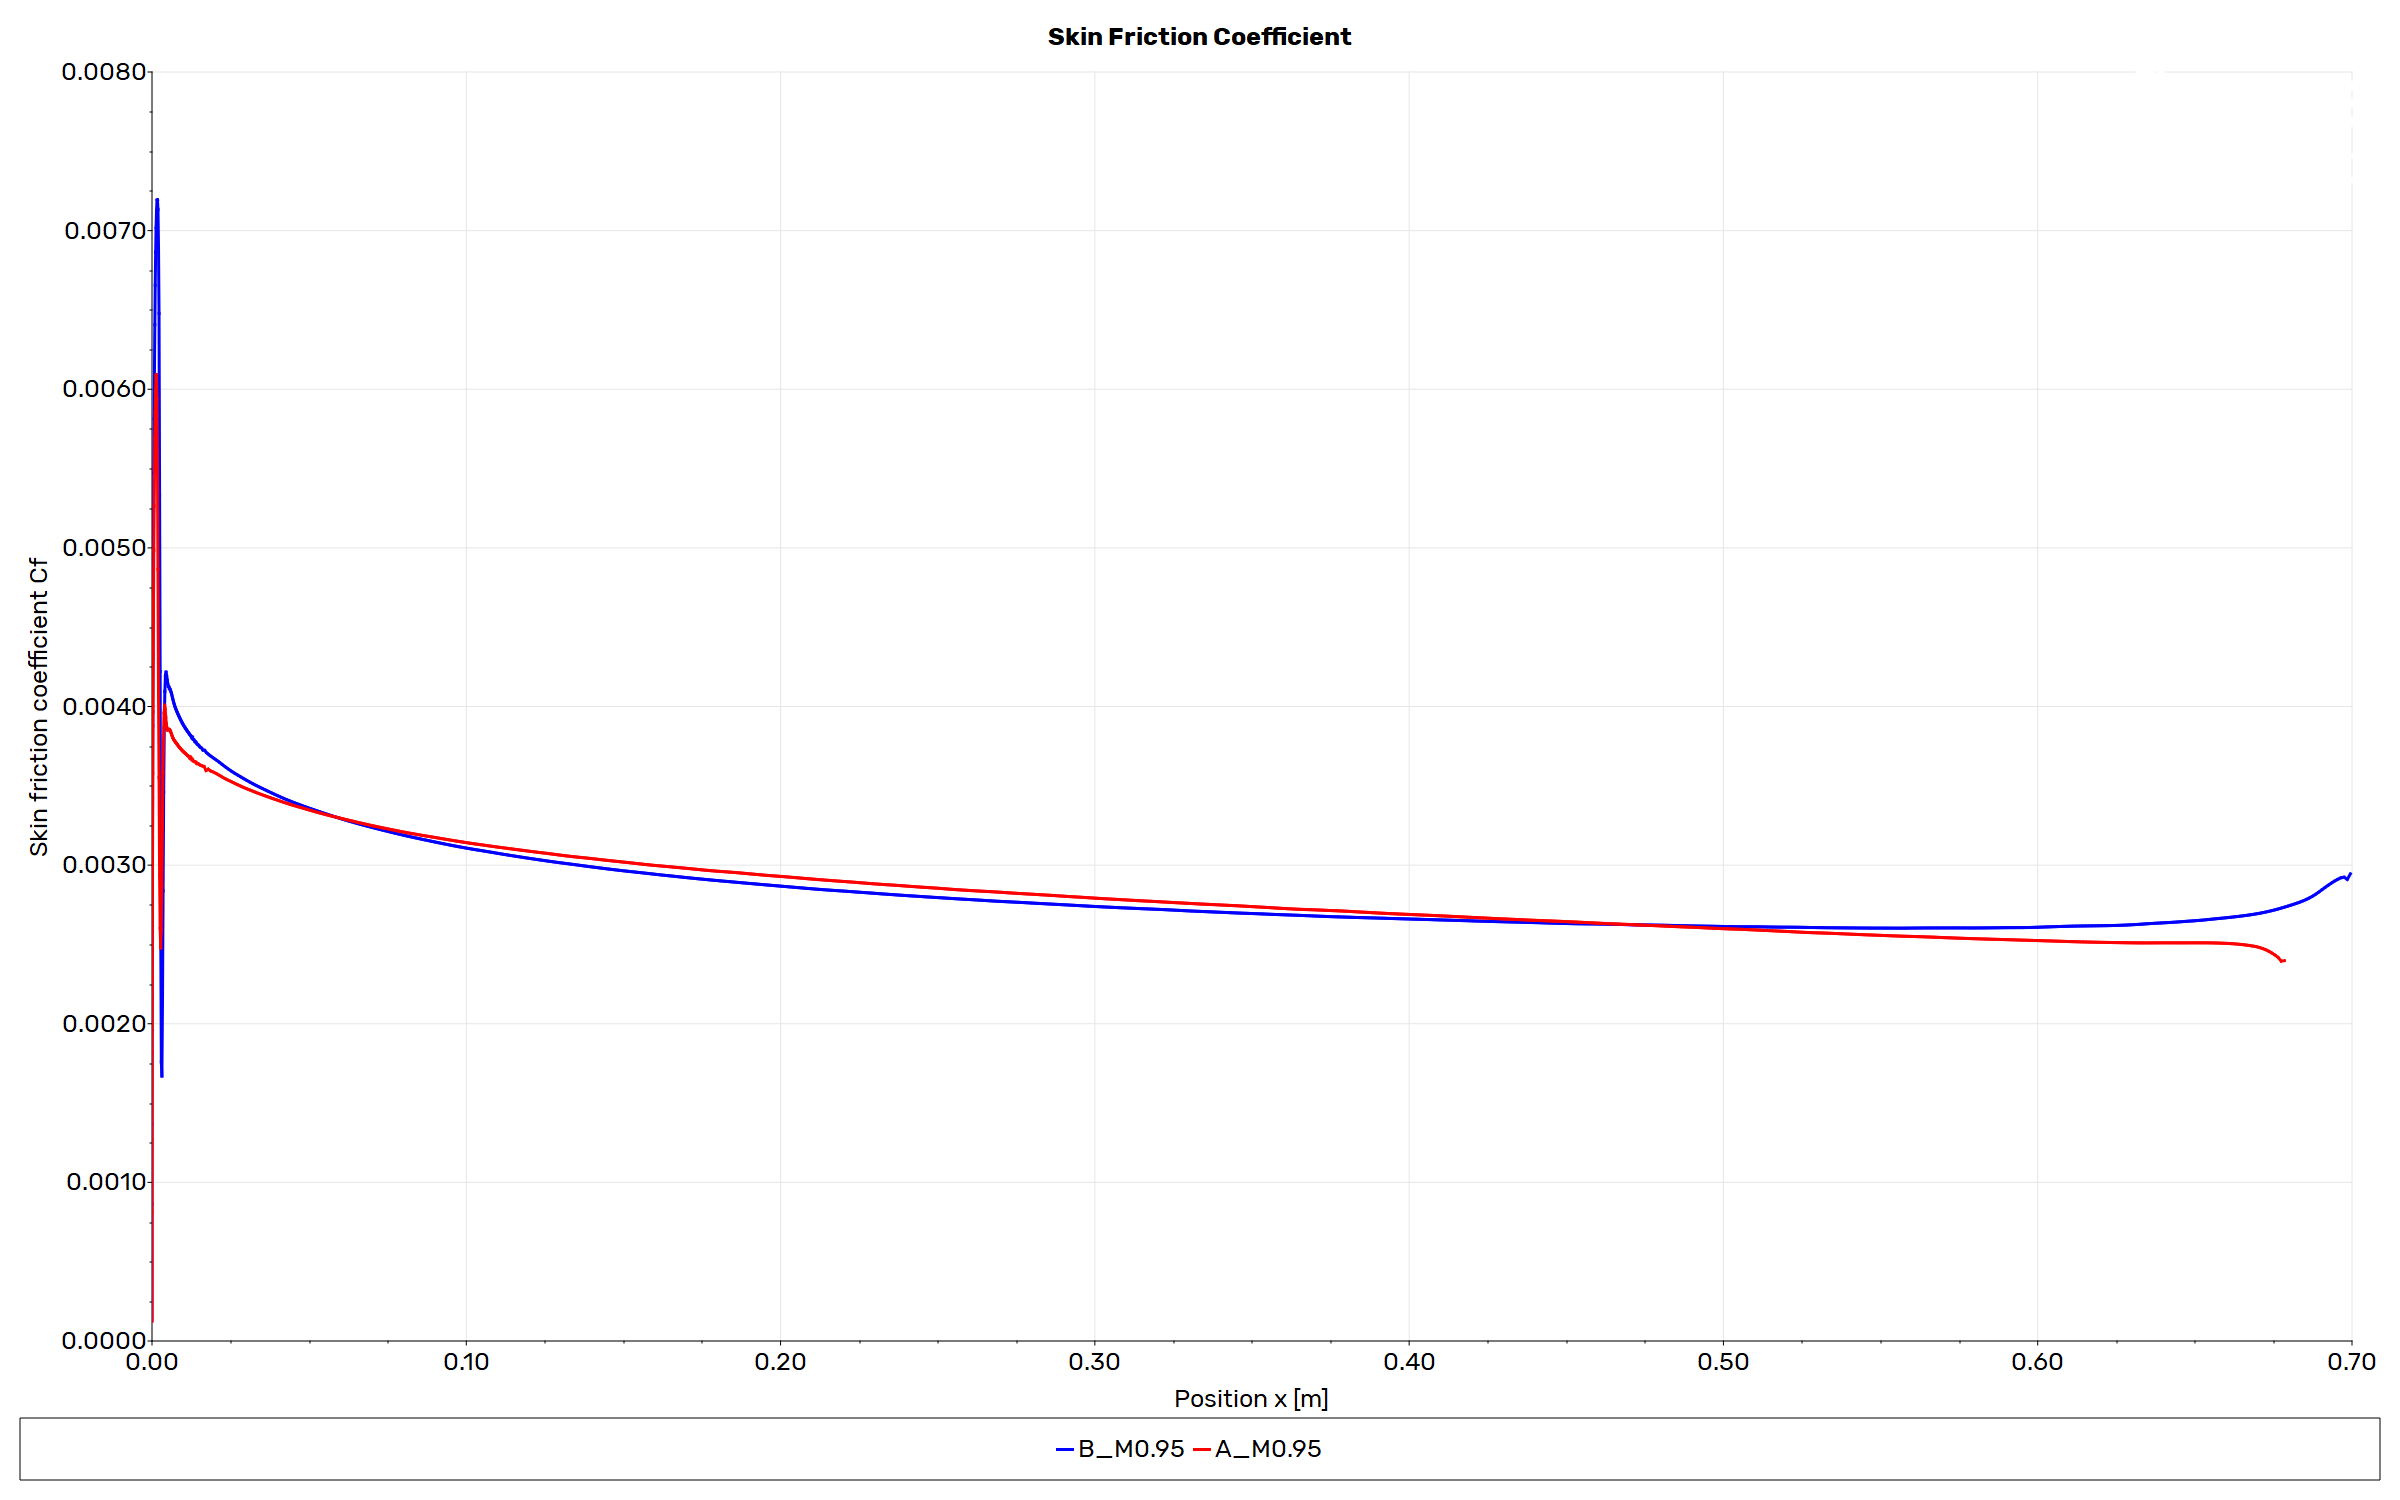
\includegraphics[width=\linewidth]{fluent_cf_AB_M0.95}
\caption{Skin-friction coefficient along the wall at \(M = 0.95\), design A (red) and B (blue), Fluent.}
\label{fig:cf}
\end{figure}

\subsection{Drag over the whole flight}

The flight model uses a drag curve against Mach number. With the start of the drag rise moved from
$M = 0.8$ to 0.94 (report~2 used 0.8), it matches Fluent at all three points within
\SI{5}{\percent} (Figure~\ref{fig:cd}; details in Appendix~\ref{app:dragmethod}). The drag force then
follows the dynamic pressure and peaks at burnout (Figure~\ref{fig:axial}). With the \SI{20}{\micro m}
roughness of the flight model the burnout drag is within \SI{2}{\percent} of Fluent's smooth wall.

\begin{figure}[H]
\centering
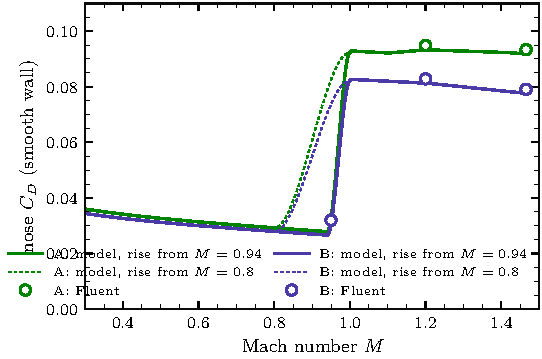
\includegraphics[width=0.75\linewidth]{fig_cd_mach}
\caption{Drag coefficient of the nose against Mach number: flight model with the old (dotted) and new
(solid) start of the drag rise, and Fluent (circles). Design A in green, B in purple; smooth wall in both.}
\label{fig:cd}
\end{figure}

\begin{figure}[H]
\centering
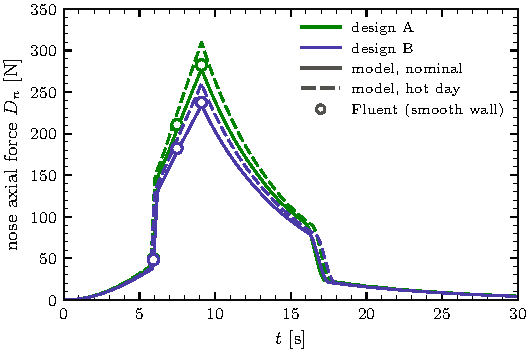
\includegraphics[width=0.75\linewidth]{fig_axial_force}
\caption{Drag of the nose during the flight (flight model, rough wall) and the Fluent points (smooth
wall).}
\label{fig:axial}
\end{figure}

\section{Loads on the structure}
\label{sec:loads}

\begin{keybox}
\begin{itemize}
\item The pressure pushes the shell \textbf{inward only at the front}: on the rounded tip at burnout (up to
\val{B-hot-LC1-dpstag}\,kPa), and on design A over the first few centimetres (up to
\val{A-hot-LC1-dpmax2}\,kPa). From mid-length to the shoulder the net pressure is \textbf{never inward}.
\item The \textbf{outward} pressure grows during the whole climb as the outside air gets thinner. At
apogee it is about \absval{A-nominal-LC3-dpmin}\,kPa on the whole shell, for both designs.
\item \textbf{Along the axis, the sealed nose is pulled off the joint at every load case.} The
overpressure inside outweighs the drag already at burnout, and at apogee the pull reaches about
\absval{B-hot-LC3-Fphi}\,N.
\item \textbf{Side force}: \val{A-nominal-LC1-Nperdeg}\,N per degree of angle of attack at burnout
(\val{B-hot-LC1-Nperdeg}\,N on a hot day), the same for both designs. It acts \val{A-xcp}\,mm (A) or
\val{B-xcp}\,mm (B) behind the tip.
\end{itemize}
\end{keybox}

\subsection{Pressure along the nose, at the three load cases}
\label{sec:pressure}

At the tip the oncoming air is stopped and presses hard on the rounded cap. The pressure falls quickly
over the first few millimetres. Further back the wall pressure is close to the outside pressure, and
slightly below it towards the shoulder, where the air speeds up onto the cylinder. The inside stays at
the pad pressure, so the rear half of the shell is pushed outward at every load case
(Figure~\ref{fig:dpx}). Over the first 10\,cm design A, with its fuller front, has about twice the
pressure of design B.

\begin{figure}[H]
\centering
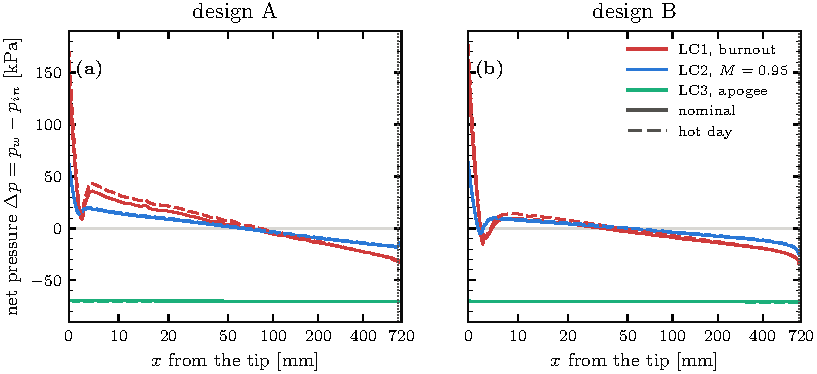
\includegraphics[width=\linewidth]{fig_dp_x}
\caption{Net pressure along the nose at the three load cases, design A (a) and design B (b). Above zero
the shell is pushed inward, below zero outward. Solid: nominal day; dashed: hot day. The $x$ axis is
stretched near the tip (logarithmic beyond 20\,mm); the dotted line is the shoulder.}
\label{fig:dpx}
\end{figure}

\begin{table}[H]
\centering
\caption{Net pressure at the three load cases [kPa]. Positive: inward, with cold inside air. Negative:
outward, with heated inside air. Each bound is the one that gives the larger load.}
\label{tab:dp_lc}
\small
\begin{tabular}{@{}lccccc@{}}
\toprule
 & \multicolumn{2}{c}{Design A} & \multicolumn{2}{c}{Design B}\\
\cmidrule(lr){2-3}\cmidrule(l){4-5}
 & Nominal & Hot day & Nominal & Hot day\\
\midrule
\grouprow{5}{LC1, burnout}
On the rounded tip (inward) & \val{A-nominal-LC1-dpstag} & \val{A-hot-LC1-dpstag} & \val{B-nominal-LC1-dpstag} & \val{B-hot-LC1-dpstag}\\
Highest behind the tip, $x > 2$\,mm (inward) & \val{A-nominal-LC1-dpmax2} & \val{A-hot-LC1-dpmax2} & \val{B-nominal-LC1-dpmax2} & \val{B-hot-LC1-dpmax2}\\
Lowest on the shell (outward) & \val{A-nominal-LC1-dpmin} & \val{A-hot-LC1-dpmin} & \val{B-nominal-LC1-dpmin} & \val{B-hot-LC1-dpmin}\\
\midrule
\grouprow{5}{LC2, transonic}
On the rounded tip (inward) & \val{A-nominal-LC2-dpstag} & \val{A-hot-LC2-dpstag} & \val{B-nominal-LC2-dpstag} & \val{B-hot-LC2-dpstag}\\
Highest behind the tip, $x > 2$\,mm (inward) & \val{A-nominal-LC2-dpmax2} & \val{A-hot-LC2-dpmax2} & \val{B-nominal-LC2-dpmax2} & \val{B-hot-LC2-dpmax2}\\
Lowest on the shell (outward) & \val{A-nominal-LC2-dpmin} & \val{A-hot-LC2-dpmin} & \val{B-nominal-LC2-dpmin} & \val{B-hot-LC2-dpmin}\\
\midrule
\grouprow{5}{LC3, apogee}
Whole shell (outward) & \val{A-nominal-LC3-dpmin} & \val{A-hot-LC3-dpmin} & \val{B-nominal-LC3-dpmin} & \val{B-hot-LC3-dpmin}\\
\bottomrule
\end{tabular}
\end{table}

\subsection{Pressure during the flight, at four stations}

Figure~\ref{fig:dpt} follows the net pressure at the four stations of Figure~\ref{fig:conventions}
through the whole flight, and Table~\ref{tab:stations} gives the extremes.
\begin{itemize}
\item The tip is pushed inward from lift-off until 15--17\,s, with the peak at burnout.
\item The other stations are pushed outward for almost the whole flight, more and more as the rocket
climbs.
\item When the shell heats the inside air, the inside pressure rises and adds a few kPa of outward
pressure during the coast (thin lines). At the shoulder of design B this gives the largest outward value
of the flight, \val{B-hot-stshoulder-min}\,kPa at \val{B-hot-stshoulder-tmin}\,s on the hot day.
\end{itemize}

\begin{figure}[H]
\centering
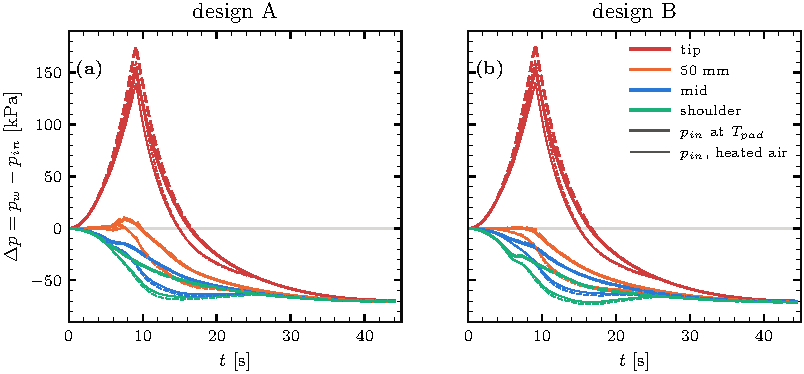
\includegraphics[width=\linewidth]{fig_dp_t}
\caption{Net pressure during the flight at the four stations, design A (a) and design B (b). Above zero
the shell is pushed inward. Thick: cold inside air; thin: heated inside air. Solid: nominal day; dashed:
hot day.}
\label{fig:dpt}
\end{figure}

\begin{table}[H]
\centering
\caption{Largest net pressure over the flight at the four stations [kPa]. Inward peaks: at the tip at
burnout, at 50\,mm at 7.2--7.5\,s ($M \approx 1.2$); 0 means never inward. Outward peaks: at apogee,
except the shoulder of design B (\val{B-hot-stshoulder-tmin}--\val{B-nominal-stshoulder-tmin}\,s).}
\label{tab:stations}
\small
\begin{tabular}{@{}lcccc@{}}
\toprule
 & \multicolumn{2}{c}{Design A} & \multicolumn{2}{c}{Design B}\\
\cmidrule(lr){2-3}\cmidrule(l){4-5}
 & Nominal & Hot day & Nominal & Hot day\\
\midrule
\grouprow{5}{Inward (cold inside air)}
Tip & \val{A-nominal-sttip-max} & \val{A-hot-sttip-max} & \val{B-nominal-sttip-max} & \val{B-hot-sttip-max}\\
50\,mm & \val{A-nominal-st50-max} & \val{A-hot-st50-max} & \val{B-nominal-st50-max} & \val{B-hot-st50-max}\\
Mid-length & \val{A-nominal-stmid-max} & \val{A-hot-stmid-max} & \val{B-nominal-stmid-max} & \val{B-hot-stmid-max}\\
Shoulder & \val{A-nominal-stshoulder-max} & \val{A-hot-stshoulder-max} & \val{B-nominal-stshoulder-max} & \val{B-hot-stshoulder-max}\\
\midrule
\grouprow{5}{Outward (heated inside air)}
Tip & \val{A-nominal-sttip-min} & \val{A-hot-sttip-min} & \val{B-nominal-sttip-min} & \val{B-hot-sttip-min}\\
50\,mm & \val{A-nominal-st50-min} & \val{A-hot-st50-min} & \val{B-nominal-st50-min} & \val{B-hot-st50-min}\\
Mid-length & \val{A-nominal-stmid-min} & \val{A-hot-stmid-min} & \val{B-nominal-stmid-min} & \val{B-hot-stmid-min}\\
Shoulder & \val{A-nominal-stshoulder-min} & \val{A-hot-stshoulder-min} & \val{B-nominal-stshoulder-min} & \val{B-hot-stshoulder-min}\\
\bottomrule
\end{tabular}
\end{table}

\subsection{Axial force on the joint}
\label{sec:forces}

Table~\ref{tab:axial} gives the \textbf{net pressure force} of the sealed nose: the outside wall pressure
minus the inside pressure, summed over the shell. It contains the pressure part of the drag and the pull
of the inside overpressure; friction is not in it. The \textbf{drag} of the nose, which is what a vented
nose would put on the joint, is in Section~\ref{sec:drag}.

\begin{table}[H]
\centering
\caption{Net pressure force on the joint at the three load cases [N]. Positive: compression, the nose is
pushed onto the joint. Negative: tension, the nose is pulled off the joint.}
\label{tab:axial}
\small
\begin{tabular}{@{}lcccc@{}}
\toprule
 & \multicolumn{2}{c}{Design A} & \multicolumn{2}{c}{Design B}\\
\cmidrule(lr){2-3}\cmidrule(l){4-5}
 & Nominal & Hot day & Nominal & Hot day\\
\midrule
\grouprow{5}{LC1, burnout}
Net pressure force, cold inside air & \val{A-nominal-LC1-Fplo} & \val{A-hot-LC1-Fplo} & \val{B-nominal-LC1-Fplo} & \val{B-hot-LC1-Fplo}\\
Net pressure force, heated inside air & \val{A-nominal-LC1-Fphi} & \val{A-hot-LC1-Fphi} & \val{B-nominal-LC1-Fphi} & \val{B-hot-LC1-Fphi}\\
\midrule
\grouprow{5}{LC2, transonic}
Net pressure force, cold inside air & \val{A-nominal-LC2-Fplo} & \val{A-hot-LC2-Fplo} & \val{B-nominal-LC2-Fplo} & \val{B-hot-LC2-Fplo}\\
Net pressure force, heated inside air & \val{A-nominal-LC2-Fphi} & \val{A-hot-LC2-Fphi} & \val{B-nominal-LC2-Fphi} & \val{B-hot-LC2-Fphi}\\
\midrule
\grouprow{5}{LC3, apogee}
Net pressure force & \val{A-nominal-LC3-Fphi} & \val{A-hot-LC3-Fphi} & \val{B-nominal-LC3-Fphi} & \val{B-hot-LC3-Fphi}\\
\bottomrule
\end{tabular}
\end{table}

At apogee the pull of about 1.8\,kN is close to the 2000\,N of Req\_07. Vent holes would bring the inside
pressure to the outside pressure and remove it; the air load on the joint would then be the drag only. The
inertial loads at the joint and the recovery load are not in this report.

\subsection{Side force under an angle of attack}
\label{sec:normal}

Fluent was run at zero angle of attack only. For a small angle of attack $\alpha$, slender-body theory gives
the side (normal) force of the nose and where it acts:
\begin{equation}
N = 2\,q\,A_{ref}\,\alpha \quad (\alpha \text{ in rad}), \qquad
M_b = N\,(x_j - x_{CP}),
\end{equation}
with $M_b$ the bending moment at the joint plane $x_j$. The force is carried mostly by the front half of the
nose (Figure~\ref{fig:normal}); the coupler carries none. ST chooses the design angle of attack (Req\_12).

\begin{table}[H]
\centering
\caption{Side force per degree of angle of attack, and its point of action.}
\label{tab:normal}
\small
\begin{tabular}{@{}llcccc@{}}
\toprule
\caseheader
\midrule
Side force at LC1, burnout & N/$^\circ$ & \val{A-nominal-LC1-Nperdeg} & \val{A-hot-LC1-Nperdeg} & \val{B-nominal-LC1-Nperdeg} & \val{B-hot-LC1-Nperdeg}\\
Side force at LC2, transonic & N/$^\circ$ & \val{A-nominal-LC2-Nperdeg} & \val{A-hot-LC2-Nperdeg} & \val{B-nominal-LC2-Nperdeg} & \val{B-hot-LC2-Nperdeg}\\
Centre of pressure $x_{CP}$, from the tip & mm & \multicolumn{2}{c}{\val{A-xcp}} & \multicolumn{2}{c}{\val{B-xcp}}\\
\bottomrule
\end{tabular}
\end{table}

\begin{figure}[H]
\centering
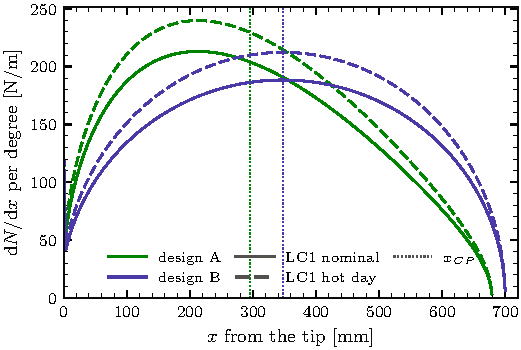
\includegraphics[width=0.75\linewidth]{fig_normal_load}
\caption{Side force per unit length and per degree of angle of attack at burnout (slender-body theory).
Dotted: centre of pressure.}
\label{fig:normal}
\end{figure}


\clearpage
\appendix
\section{How the numbers were obtained}
\label{app:method}

\subsection{Flight model and Fluent points}

The trajectory comes from the Python design tool (report~2), flown with the nose of each design. Along it,
\begin{equation}
q = \tfrac12\,\rho_\infty V^2 = \tfrac12\,\gamma\,p_\infty M^2, \qquad
T_0 = T_\infty\left(1 + \tfrac{\gamma - 1}{2}\,M^2\right).
\end{equation}
Nominal day: \SI{\val{pad-T}}{K} on the pad, propellant mass from the total impulse. Hot day:
\SI{\val{pad-Thot}}{K} on the pad and the LVO masses.

The three Fluent runs use the free stream of design~A's nominal trajectory (Table~\ref{tab:points}).
Design~B is run at the same points, so that A and B differ by shape only (B's own burnout is at
$M = \val{B-own-burnout-M}$).

\begin{table}[H]
\centering
\caption{Free stream of the Fluent runs. Reynolds number per metre: $\rho_\infty V/\mu_\infty$.}
\label{tab:points}
\small
\begin{tabular}{@{}lccc@{}}
\toprule
 & Transonic & Supersonic & Burnout\\
\midrule
Time $t$ [s] & \val{pt-M095-t} & \val{pt-M120-t} & \val{pt-M147-t}\\
Altitude $z$ [m] & \val{pt-M095-z} & \val{pt-M120-z} & \val{pt-M147-z}\\
Mach number $M$ & \val{pt-M095-M} & \val{pt-M120-M} & \val{pt-M147-M}\\
Static pressure $p_\infty$ [Pa] & \val{pt-M095-p} & \val{pt-M120-p} & \val{pt-M147-p}\\
Static temperature $T_\infty$ [K] & \val{pt-M095-T} & \val{pt-M120-T} & \val{pt-M147-T}\\
Dynamic pressure $q$ [kPa] & \val{pt-M095-q} & \val{pt-M120-q} & \val{pt-M147-q}\\
Reynolds number per metre [$10^6$/m] & \val{pt-M095-Re} & \val{pt-M120-Re} & \val{pt-M147-Re}\\
\bottomrule
\end{tabular}
\end{table}

\begin{table}[H]
\centering
\caption{Geometry of the two noses. $L$: Haack length to the sharp apex; the \SI{4.5}{mm} spherical tip
removes $\delta$, so the curved part is $x_S = L - \delta$ long.}
\label{tab:designs}
\small
\begin{tabular}{@{}lcc@{}}
\toprule
 & A (baseline) & B (backup)\\
\midrule
Profile & LV-Haack ($C = 1/3$) & Von K\'arm\'an ($C = 0$)\\
$L$ / $\delta$ [mm] & \val{A-L} / \val{A-delta} & \val{B-L} / \val{B-delta}\\
Curved part $x_S$ + coupler $c$ [mm] & \val{A-xS} + \val{A-c} & \val{B-xS} + \val{B-c}\\
Fineness $L/D$ & \val{A-fineness} & \val{B-fineness}\\
\bottomrule
\end{tabular}
\end{table}

\subsection{Drag}
\label{app:dragmethod}

The axial force is integrated over the Fluent wall faces, with $r$ the local radius:
\begin{equation}
F_p = \sum (p_w - p_\infty)\,2\pi r\,\mathrm{d}r, \qquad
F_v = \sum \tau_w\,2\pi r\,\mathrm{d}x, \qquad
C_D = \frac{F_p + F_v}{q\,A_{ref}}, \quad A_{ref} = \pi R^2 = \SI{0.025447}{m^2}.
\end{equation}
The sums reproduce Fluent's own force report to \SI{0.1}{N}. The net pressure force of the sealed nose
(Table~\ref{tab:axial}) is $\sum (p_w - p_{in})\,2\pi r\,\mathrm{d}r = F_p + (p_\infty - p_{in})\,A_{ref}$.

The flight model (report~2) adds a wave drag from Euler simulations and a flat-plate friction,
\begin{equation}
C_{D,n}(M) = C_{D,w}(M) + C_f\,\frac{S_{wet}}{A_{ref}}, \qquad
C_{D,w}(M) = C_{D,w}(1.1)\,s^2(3 - 2s), \quad s = \frac{M - M_{on}}{1 - M_{on}} \in [0, 1]
\end{equation}
below $M = 1.1$. Report~2 used $M_{on} = 0.8$, which gave 2.6 times Fluent's drag at $M = 0.95$
(\val{A-cdold-M095} against \val{A-cd-M095}). With $M_{on} = 0.94$ the model matches Fluent at all three
points:
\begin{center}\small
\begin{tabular}{@{}lccc@{}}
\toprule
Fluent / model $- 1$ & $M = 0.95$ & 1.20 & \val{pt-M147-M}\\
\midrule
A & \val{A-dcd-M095}\,\% & \val{A-dcd-M120}\,\% & \val{A-dcd-M147}\,\%\\
B & \val{B-dcd-M095}\,\% & \val{B-dcd-M120}\,\% & \val{B-dcd-M147}\,\%\\
\bottomrule
\end{tabular}
\end{center}
The change raises the apogee by \SI{7}{m} (A) and \SI{1}{m} (B). Along the flight,
$D_n(t) = q(t)\,A_{ref}\,C_{D,n}\bigl(M(t)\bigr)$, with the friction of a \SI{20}{\micro m} rough wall and
the coupler included.

\subsection{Side force}

Under a small angle of attack $\alpha$ [rad], slender-body theory gives, with $S(x) = \pi r(x)^2$ and $V_n$
the volume of the nose,
\begin{equation}
\frac{\mathrm{d}N}{\mathrm{d}x} = 2\,q\,\alpha\,\frac{\mathrm{d}S}{\mathrm{d}x}, \qquad
N = 2\,q\,A_{ref}\,\alpha, \qquad
x_{CP} = x_S - \frac{V_n}{A_{ref}}.
\end{equation}

\subsection{Heating}
\label{app:heatmethod}

From the two Fluent runs at burnout (adiabatic wall, wall at \SI{300}{K}):
\begin{equation}
h(x) = \frac{q_w(x)}{T_{aw}(x) - \SI{300}{K}}, \qquad r(x) = \frac{T_{aw}(x) - T_\infty}{T_0 - T_\infty}.
\end{equation}
The recovery factor $r$ is \val{A-recovery} (A) and \val{B-recovery} (B) on the shell.

The flight model of report~1 uses
\begin{gather}
h_s = 0.763\,\mathrm{Pr}^{-0.6}\sqrt{\rho_s\,\mu(T_0)\,\frac{\mathrm{d}u_e}{\mathrm{d}x}}\;c_p, \quad
\frac{\mathrm{d}u_e}{\mathrm{d}x} = \frac{1}{r_n}\sqrt{\frac{2(p_0 - p_\infty)}{\rho_s}}
\quad\text{(tip, Fay--Riddell)},\\
h_t = \mathrm{St}\,\rho^* V c_p, \quad \mathrm{St} = 0.0296\,\mathrm{Re}_x^{*\,-0.2}\,\mathrm{Pr}^{-2/3},
\quad T_r = T_\infty\left(1 + r\,\tfrac{\gamma - 1}{2}M^2\right),\ r = \mathrm{Pr}^{1/3}
\quad\text{(shell, Eckert)},
\end{gather}
with $\rho^*$, $\mathrm{Re}_x^*$ at Eckert's reference temperature
$T^* = T_\infty(1 + 0.032M^2 + 0.58(T_w/T_\infty - 1))$.

At burnout the model and Fluent can be compared directly (Figure~\ref{fig:hcal}). Without any correction
the model is already within \SI{6}{\percent} of Fluent at the tip and along the shell. Three small
factors bring it onto Fluent (Table~\ref{tab:calibfull}).

\begin{figure}[H]
\centering
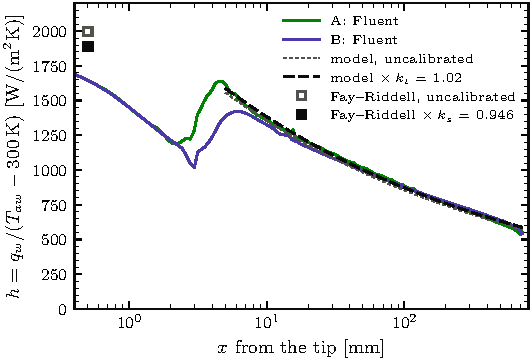
\includegraphics[width=0.75\linewidth]{fig_h_calibration}
\caption{Heat-transfer coefficient at burnout on a \SI{300}{K} wall: Fluent for A and B (smoothed between
3 and 15\,mm), the model of the shell before and after calibration (lines), and the model of the tip
before and after calibration (squares, placed at 0.5\,mm).}
\label{fig:hcal}
\end{figure}

\begin{table}[H]
\centering
\caption{Fluent against the uncalibrated model at burnout, wall at \SI{300}{K}, and the factor used in the
flight model.}
\label{tab:calibfull}
\small
\begin{tabular}{@{}lccc@{}}
\toprule
Fluent / model & A & B & Factor\\
\midrule
Heat flux at the tip & \val{A-ratio-s} & \val{B-ratio-s} & $k_s = \val{ks}$\\
$h$ along the shell, 50\,mm to shoulder (median, 10--90\,\%) & \val{A-ratio-t} (\val{A-ratio-t-lo}--\val{A-ratio-t-hi}) & \val{B-ratio-t} (\val{B-ratio-t-lo}--\val{B-ratio-t-hi}) & $k_t = \val{kt}$\\
Heat into the first \val{tip-length}\,mm (tip insert) [W] & \val{A-Qtip-fluent} / \val{A-Qtip-model} & \val{B-Qtip-fluent} / \val{B-Qtip-model} & $k_{tip} = \val{ktip}$\\
\bottomrule
\end{tabular}
\end{table}

The lumped tip insert takes its side heating at $x_{tip}/2$, which misses the high $h$ just behind the
spherical cap; with $k_s$ and $k_t$ applied it still gets 13--\SI{15}{\percent} too little heat, hence
$k_{tip}$. Fluent's recovery factor (\val{A-recovery}) is a little above the model's
$\mathrm{Pr}^{1/3} = \val{recovery-model}$, so the model's driving temperature on the shell
($T_r = \SI{\val{Tr-model}}{K}$) is 1--\SI{4}{K} below Fluent's $T_{aw}$.

With the calibrated $h$, two wall models are integrated along the trajectories:
\begin{itemize}
\item \textbf{shell}: one-dimensional conduction through the CFRP, heated outside, adiabatic inside,
\begin{equation}
\rho c\,\frac{\partial T}{\partial t} = k\,\frac{\partial^2 T}{\partial y^2}, \qquad
-k\frac{\partial T}{\partial y}\Big|_{out} = h\,(T_r - T_w), \qquad \frac{\partial T}{\partial y}\Big|_{in} = 0;
\end{equation}
run at 50\,mm for the histories of Section~\ref{sec:heating} and at 22 stations from 10\,mm to the shoulder
for the thermal profile (\file{report_720/thermal_profile.py});
\item \textbf{Al tip insert}: one temperature (aluminium conducts fast),
\begin{equation}
m\,c\,\frac{\mathrm{d}T}{\mathrm{d}t} = k_{tip}\left[0.55\,h_s A_{cap}(T_0 - T) + h_t(x_{tip}/2)\,A_{lat}(T_r - T)\right].
\end{equation}
\end{itemize}
The inside air (upper bound) is the mean inner-face temperature at 50\,mm, mid-length and shoulder, never
below the pad temperature.

\section{Quality of the runs}
\label{app:setup}

\begin{itemize}
\item \textbf{Convergence}: $(\max C_D - \min C_D)/\overline{C_D}$ of \zone{wall\_nose} over the last 500
iterations is \val{conv-lo}--\val{conv-hi}\,\% in all eight runs, below the \SI{0.1}{\percent} of REPORT-4
(Figure~\ref{fig:cdhist}).
\item \textbf{Wall resolution}: over the eight runs, the largest $y^+$ is \val{yplus-nose} on the nose and
\val{yplus-coupler} on the coupler (Figure~\ref{fig:yplus} shows burnout), so the boundary layer is resolved
down to the wall as SST requires.
\item \textbf{Mesh}: the REPORT-4 recipe, 174\,380 (A) and 174\,155 (B) cells, maximum skewness 0.90 and
0.94. No mesh study was made for these two noses; the recipe was checked on study~A only.
\end{itemize}

\begin{figure}[H]
\centering
\begin{subfigure}[t]{0.49\linewidth}
\centering
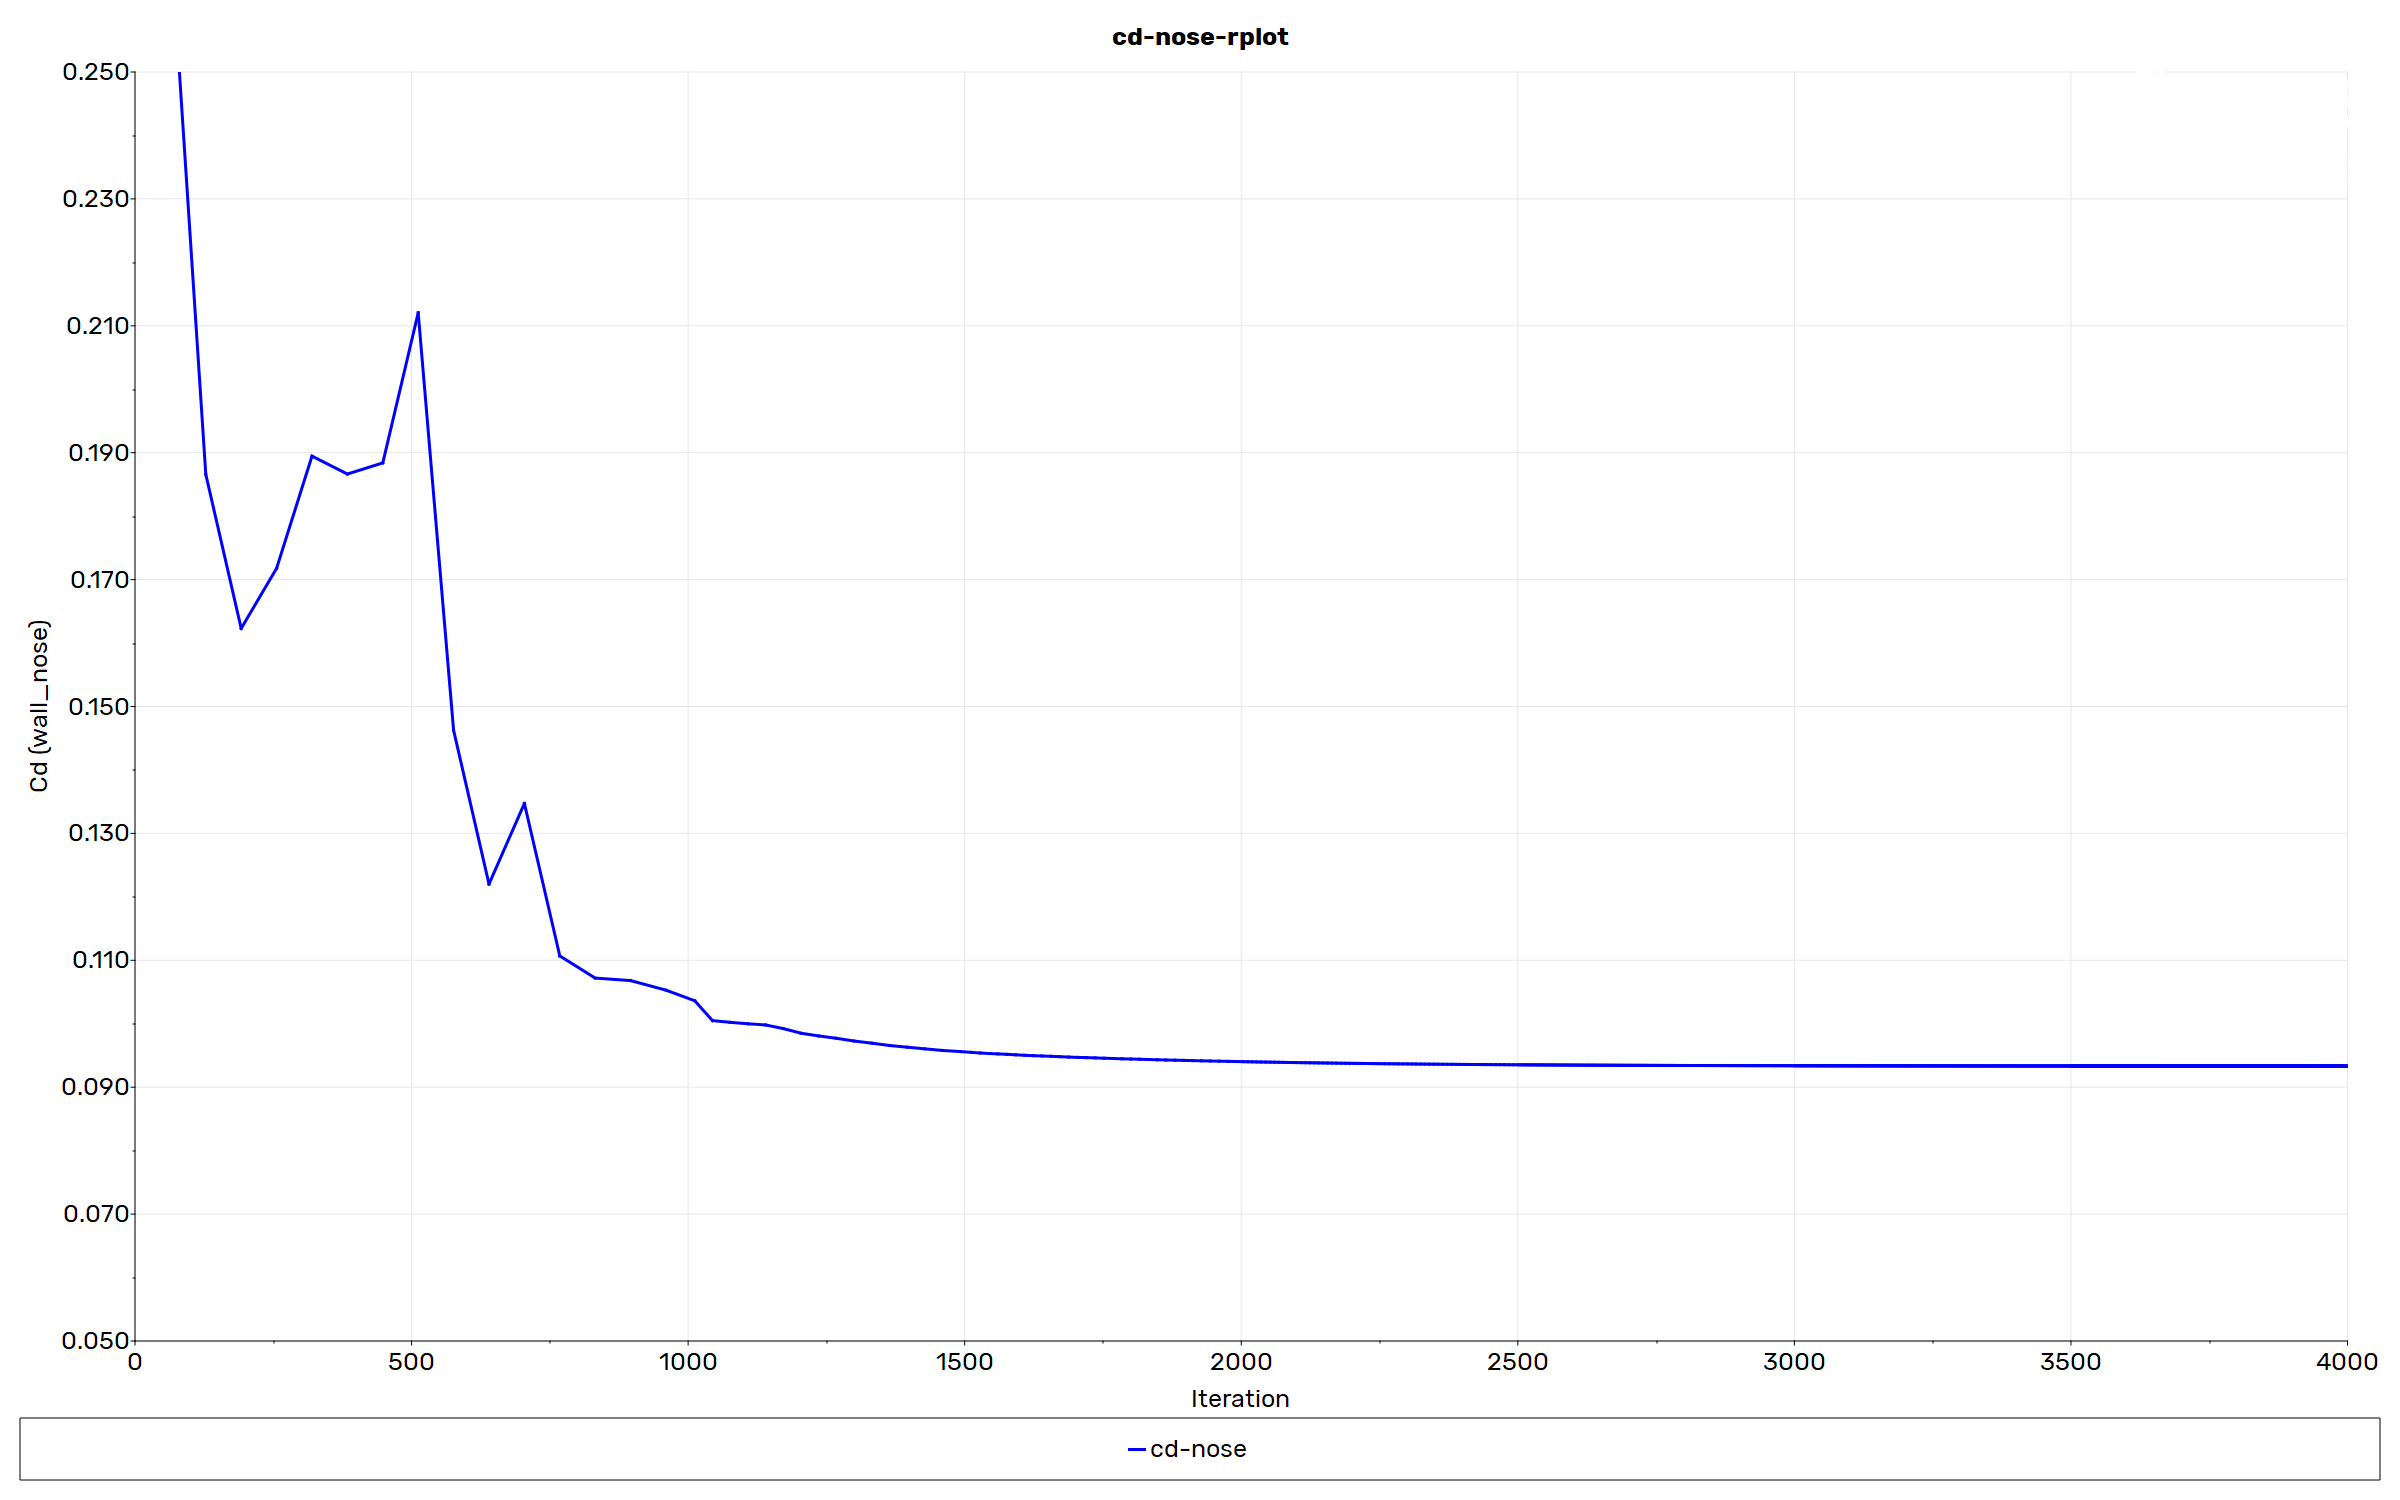
\includegraphics[width=\linewidth]{fluent_cd_A_adiab}
\caption{Design A, burnout.}
\end{subfigure}\hfill
\begin{subfigure}[t]{0.49\linewidth}
\centering
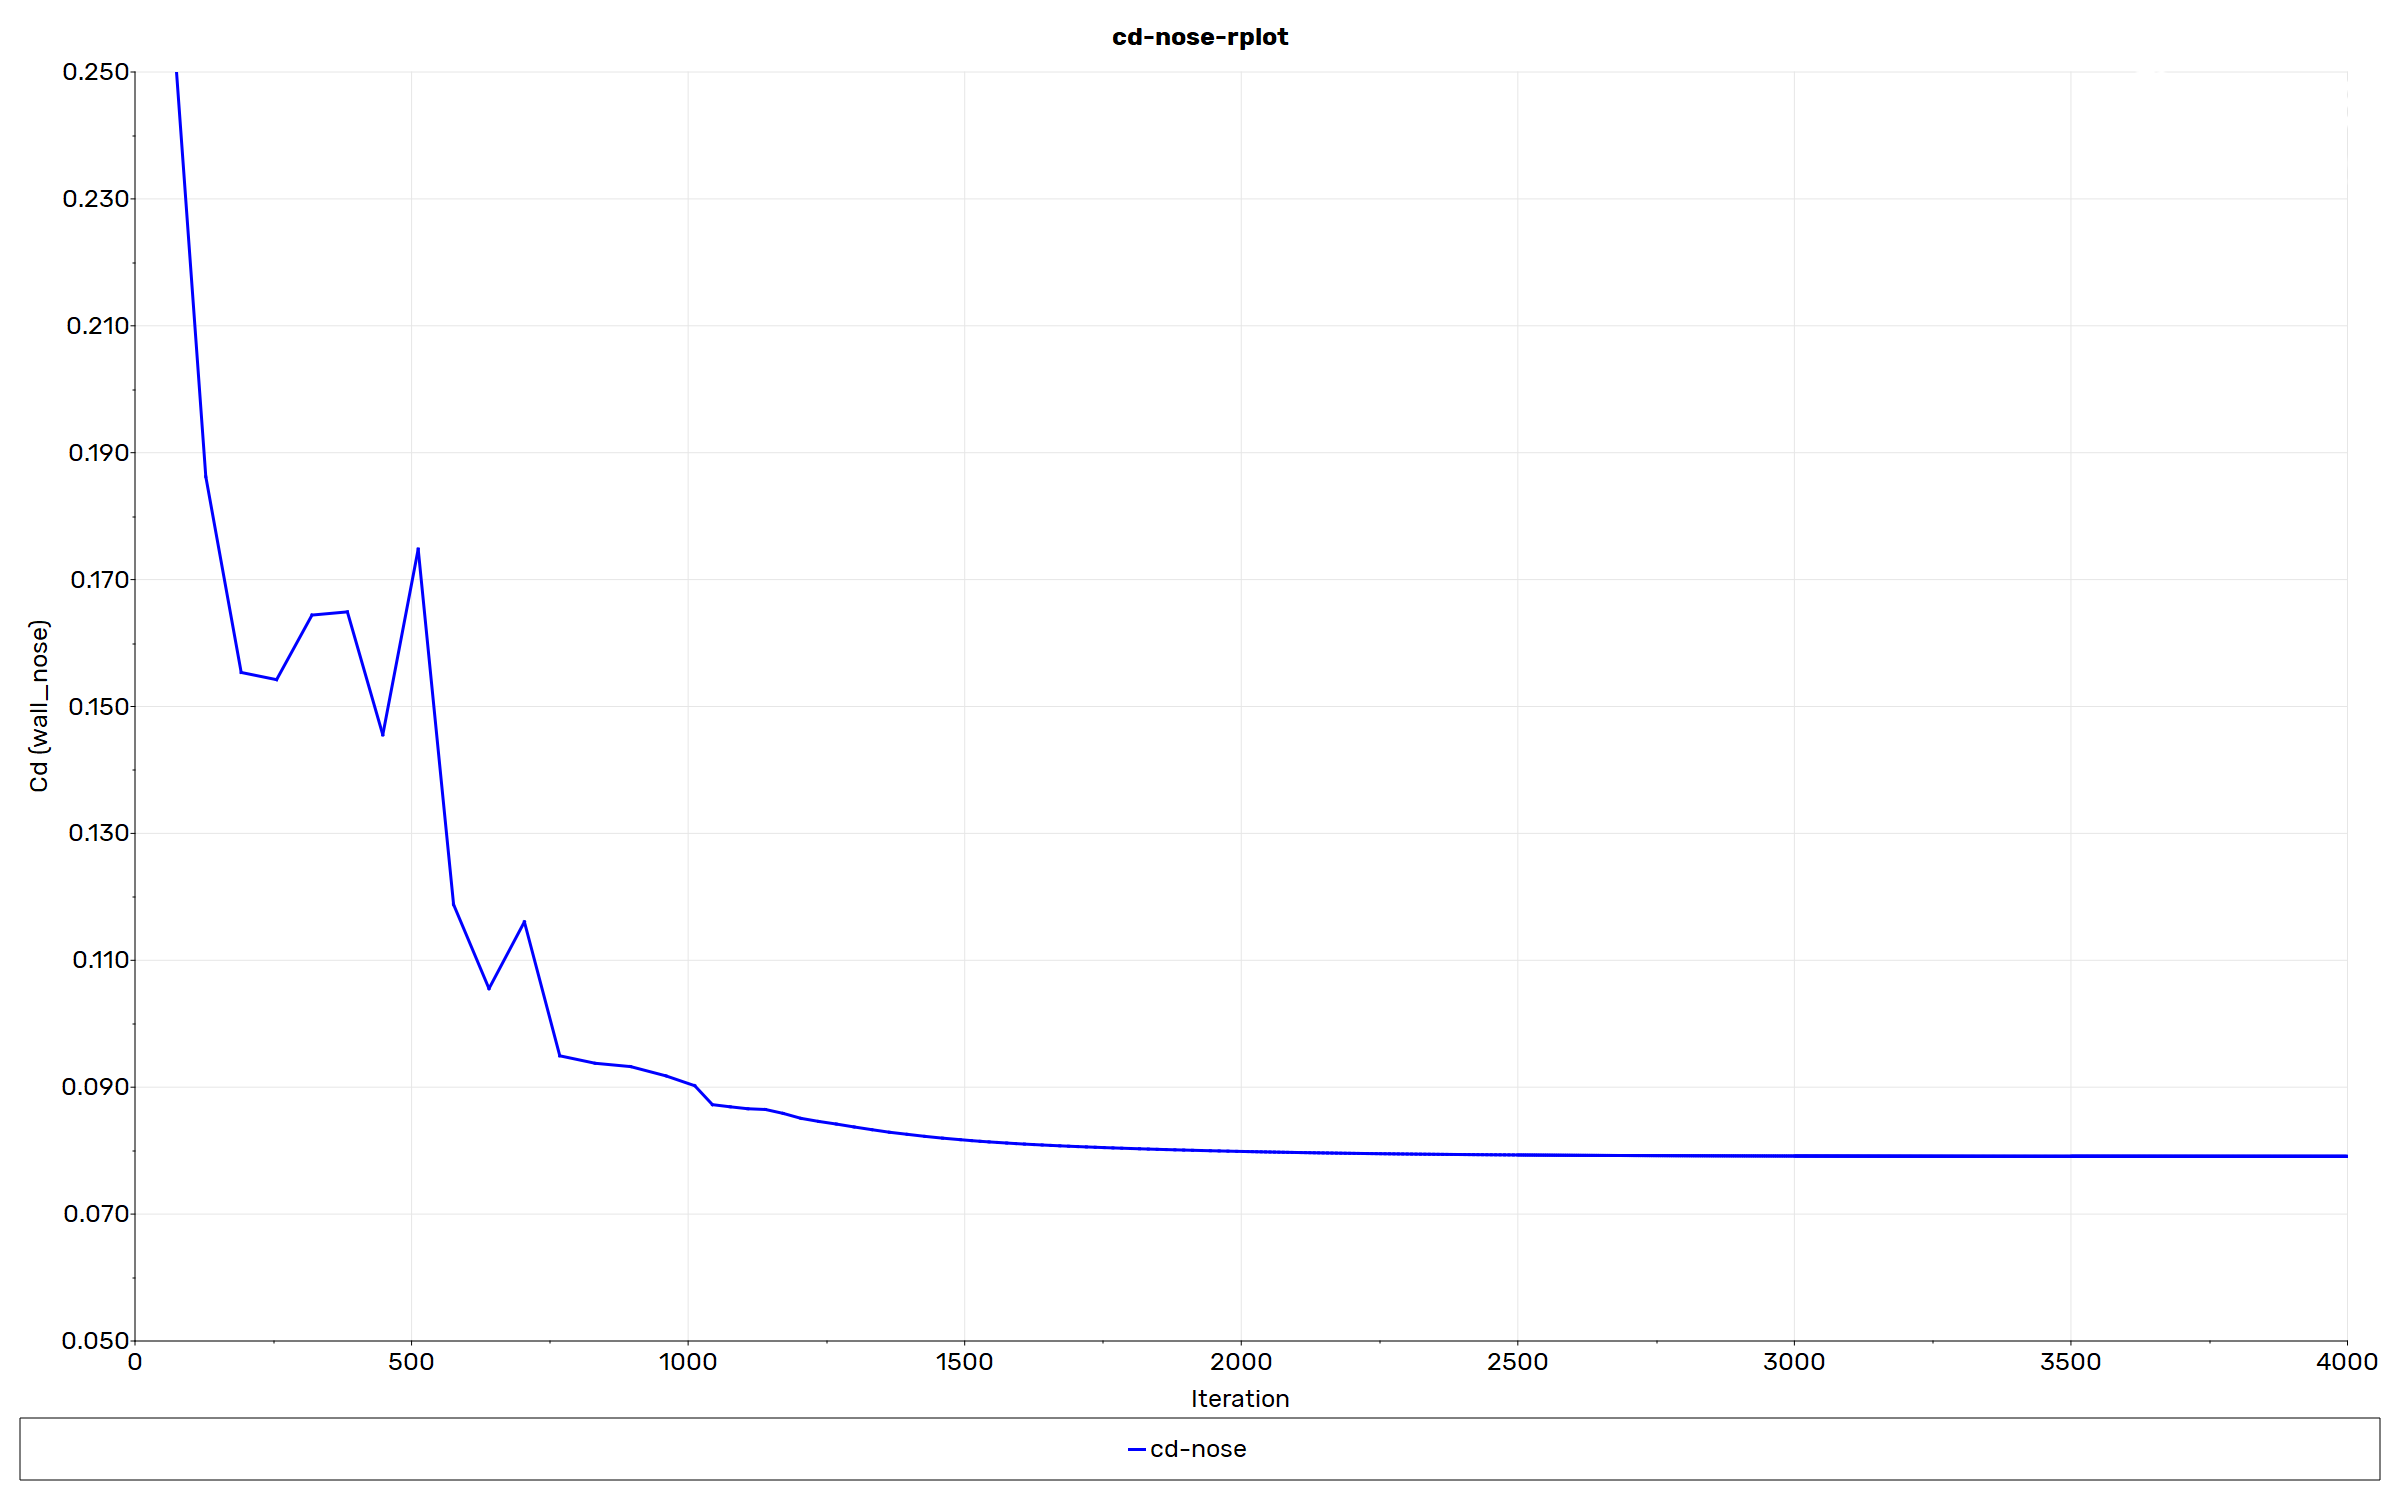
\includegraphics[width=\linewidth]{fluent_cd_B_adiab}
\caption{Design B, burnout.}
\end{subfigure}
\caption{Drag coefficient against iterations (Fluent).}
\label{fig:cdhist}
\end{figure}

\begin{figure}[H]
\centering
\begin{subfigure}[t]{0.49\linewidth}
\centering
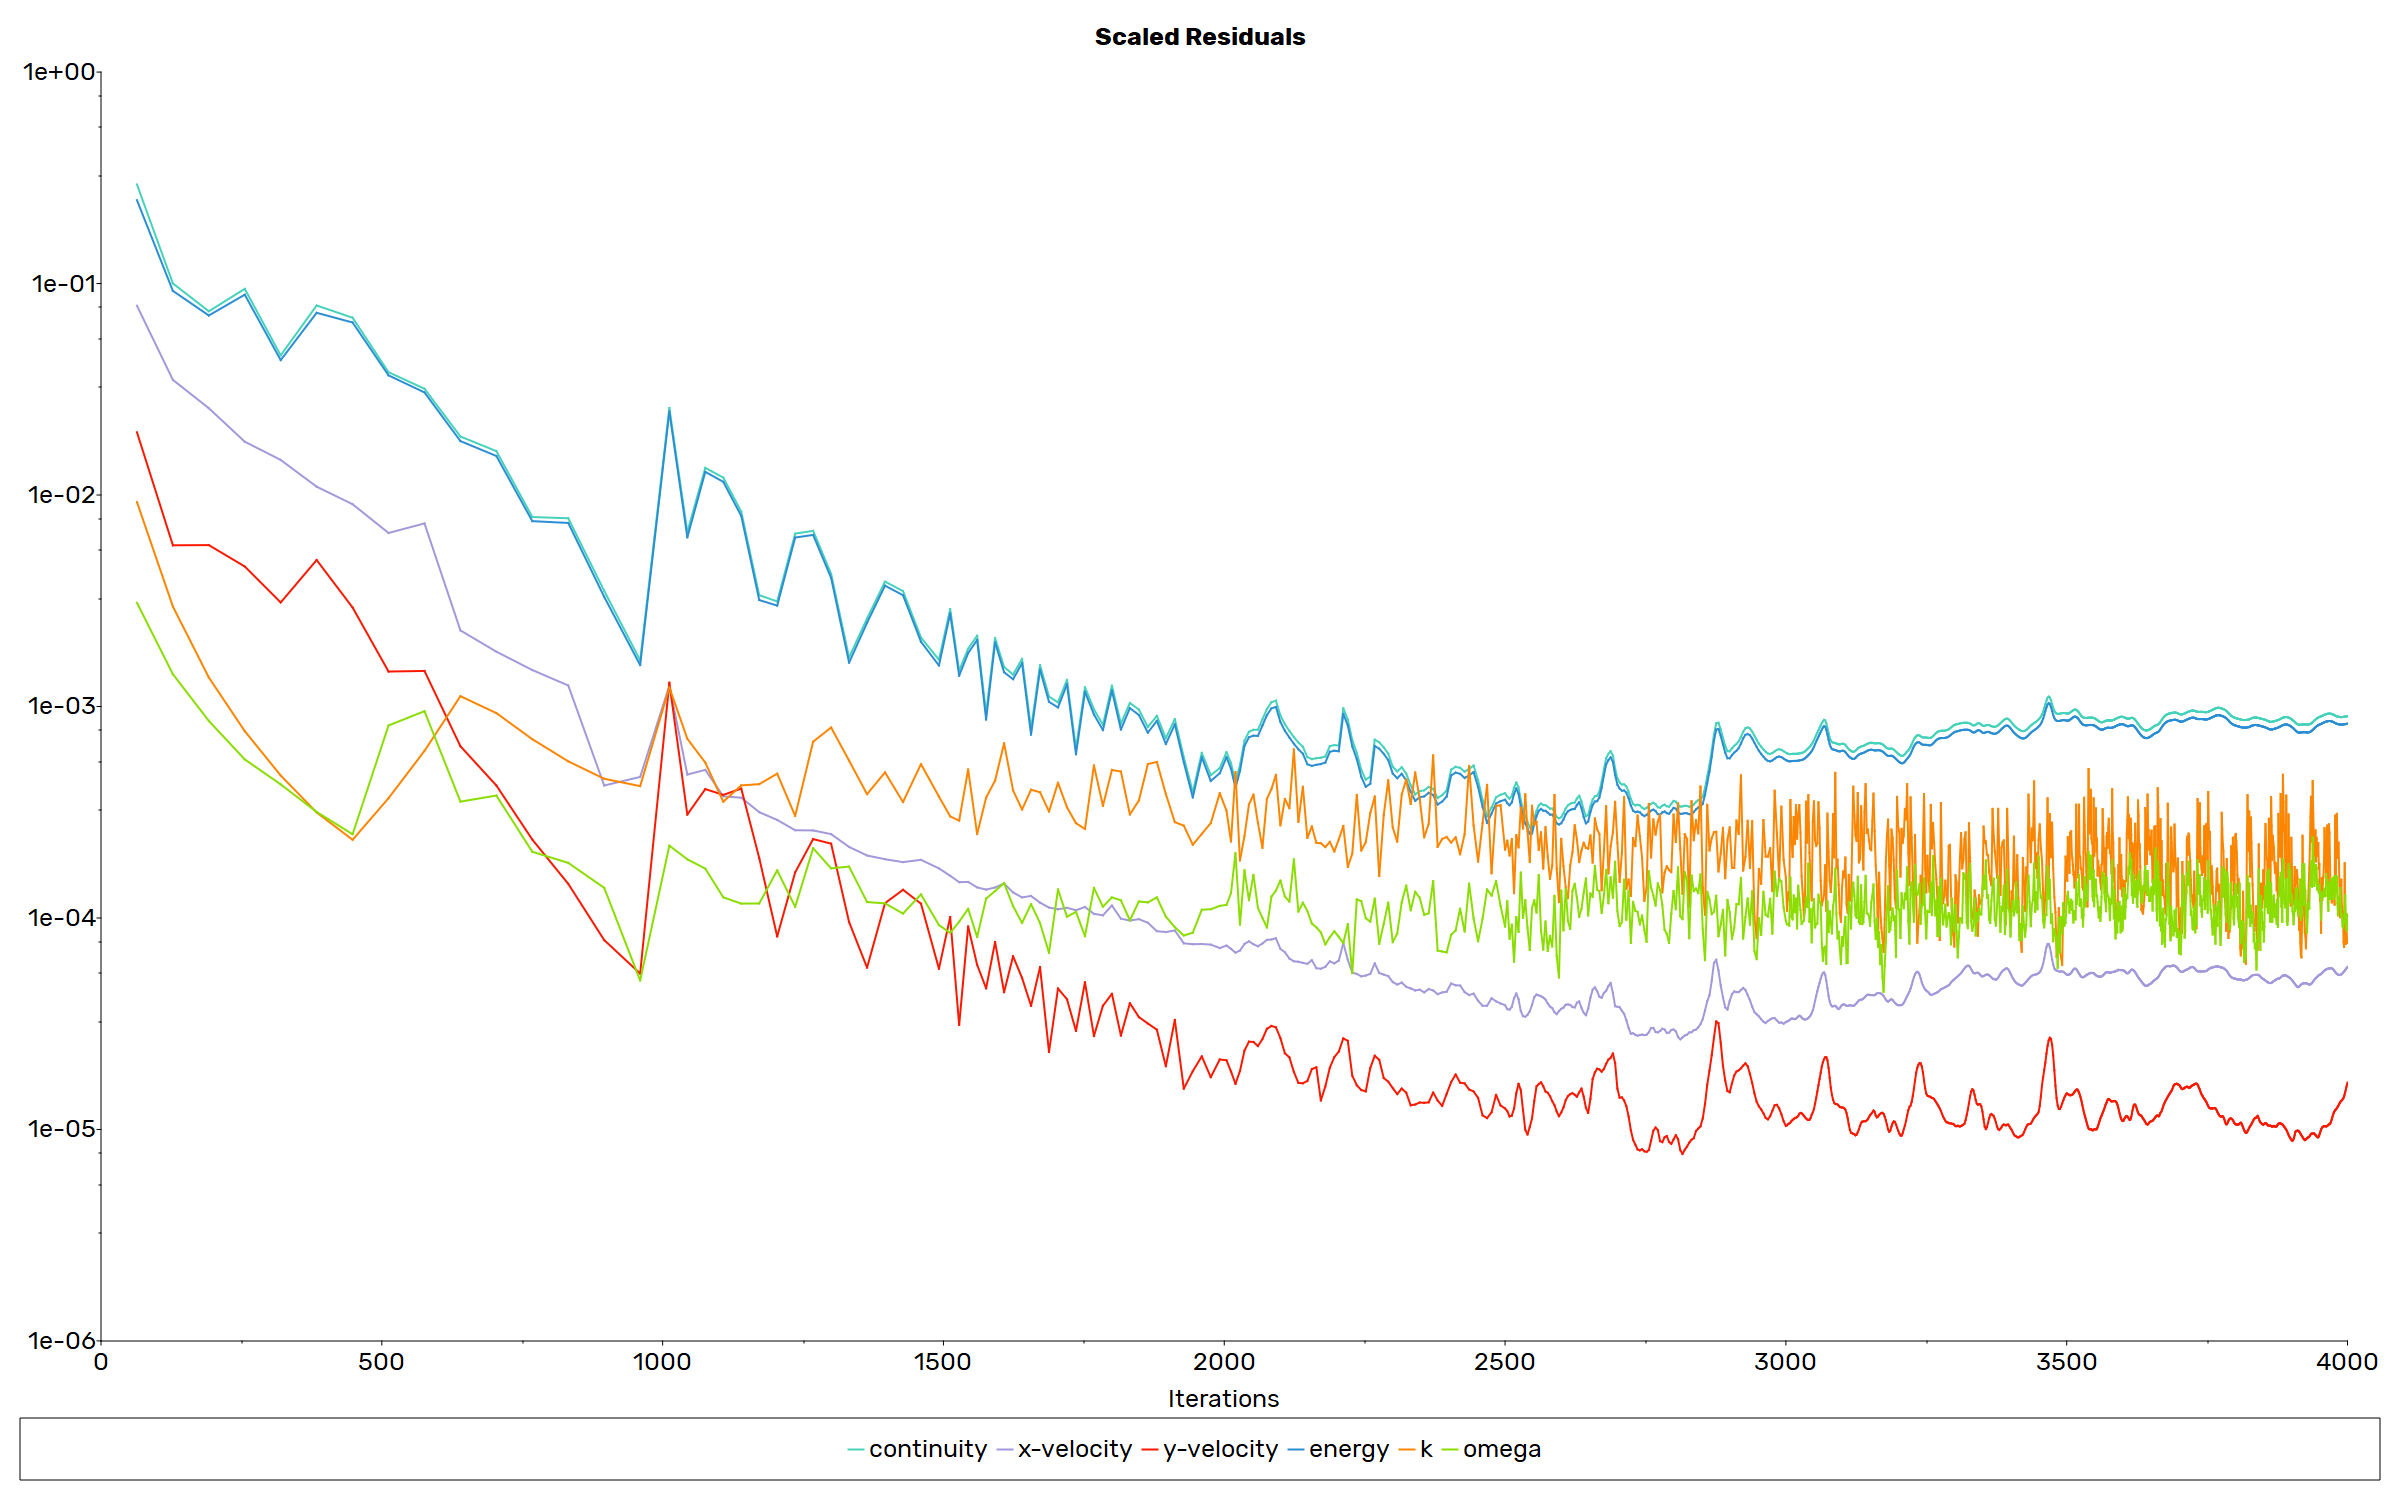
\includegraphics[width=\linewidth]{fluent_residuals_A_adiab}
\caption{Design A, burnout.}
\end{subfigure}\hfill
\begin{subfigure}[t]{0.49\linewidth}
\centering
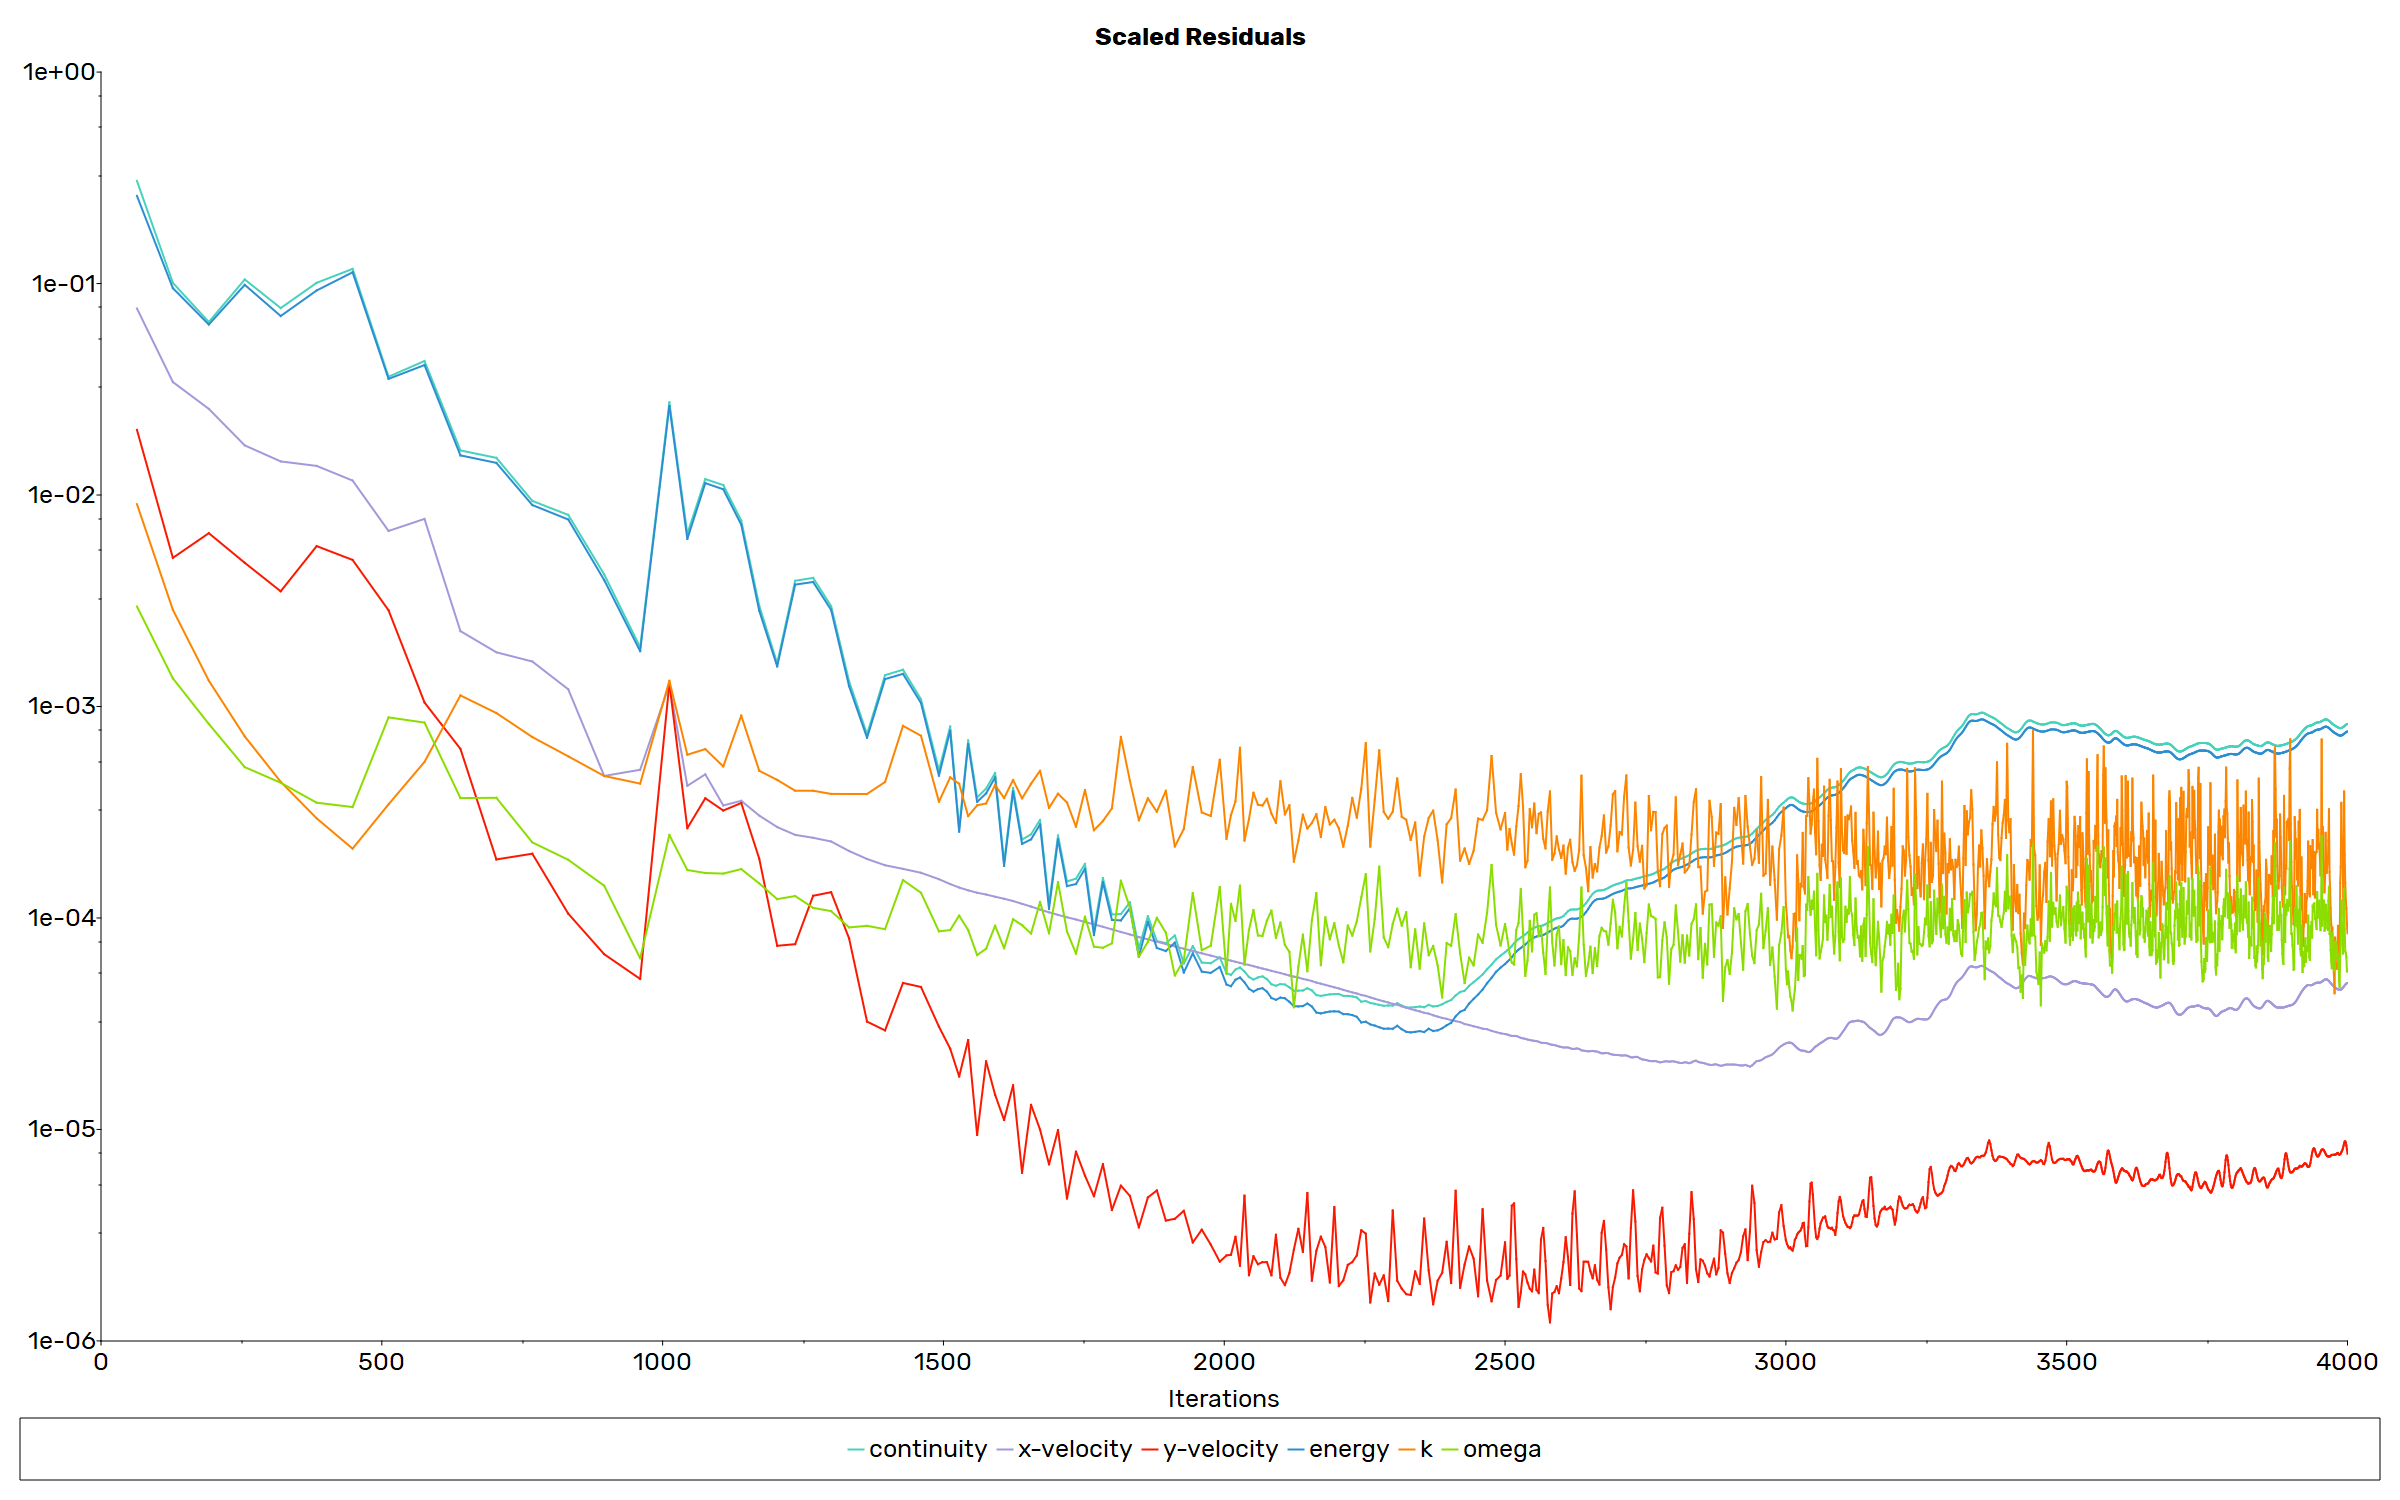
\includegraphics[width=\linewidth]{fluent_residuals_B_adiab}
\caption{Design B, burnout.}
\end{subfigure}
\caption{Residuals against iterations (Fluent).}
\label{fig:residuals}
\end{figure}

\begin{figure}[H]
\centering
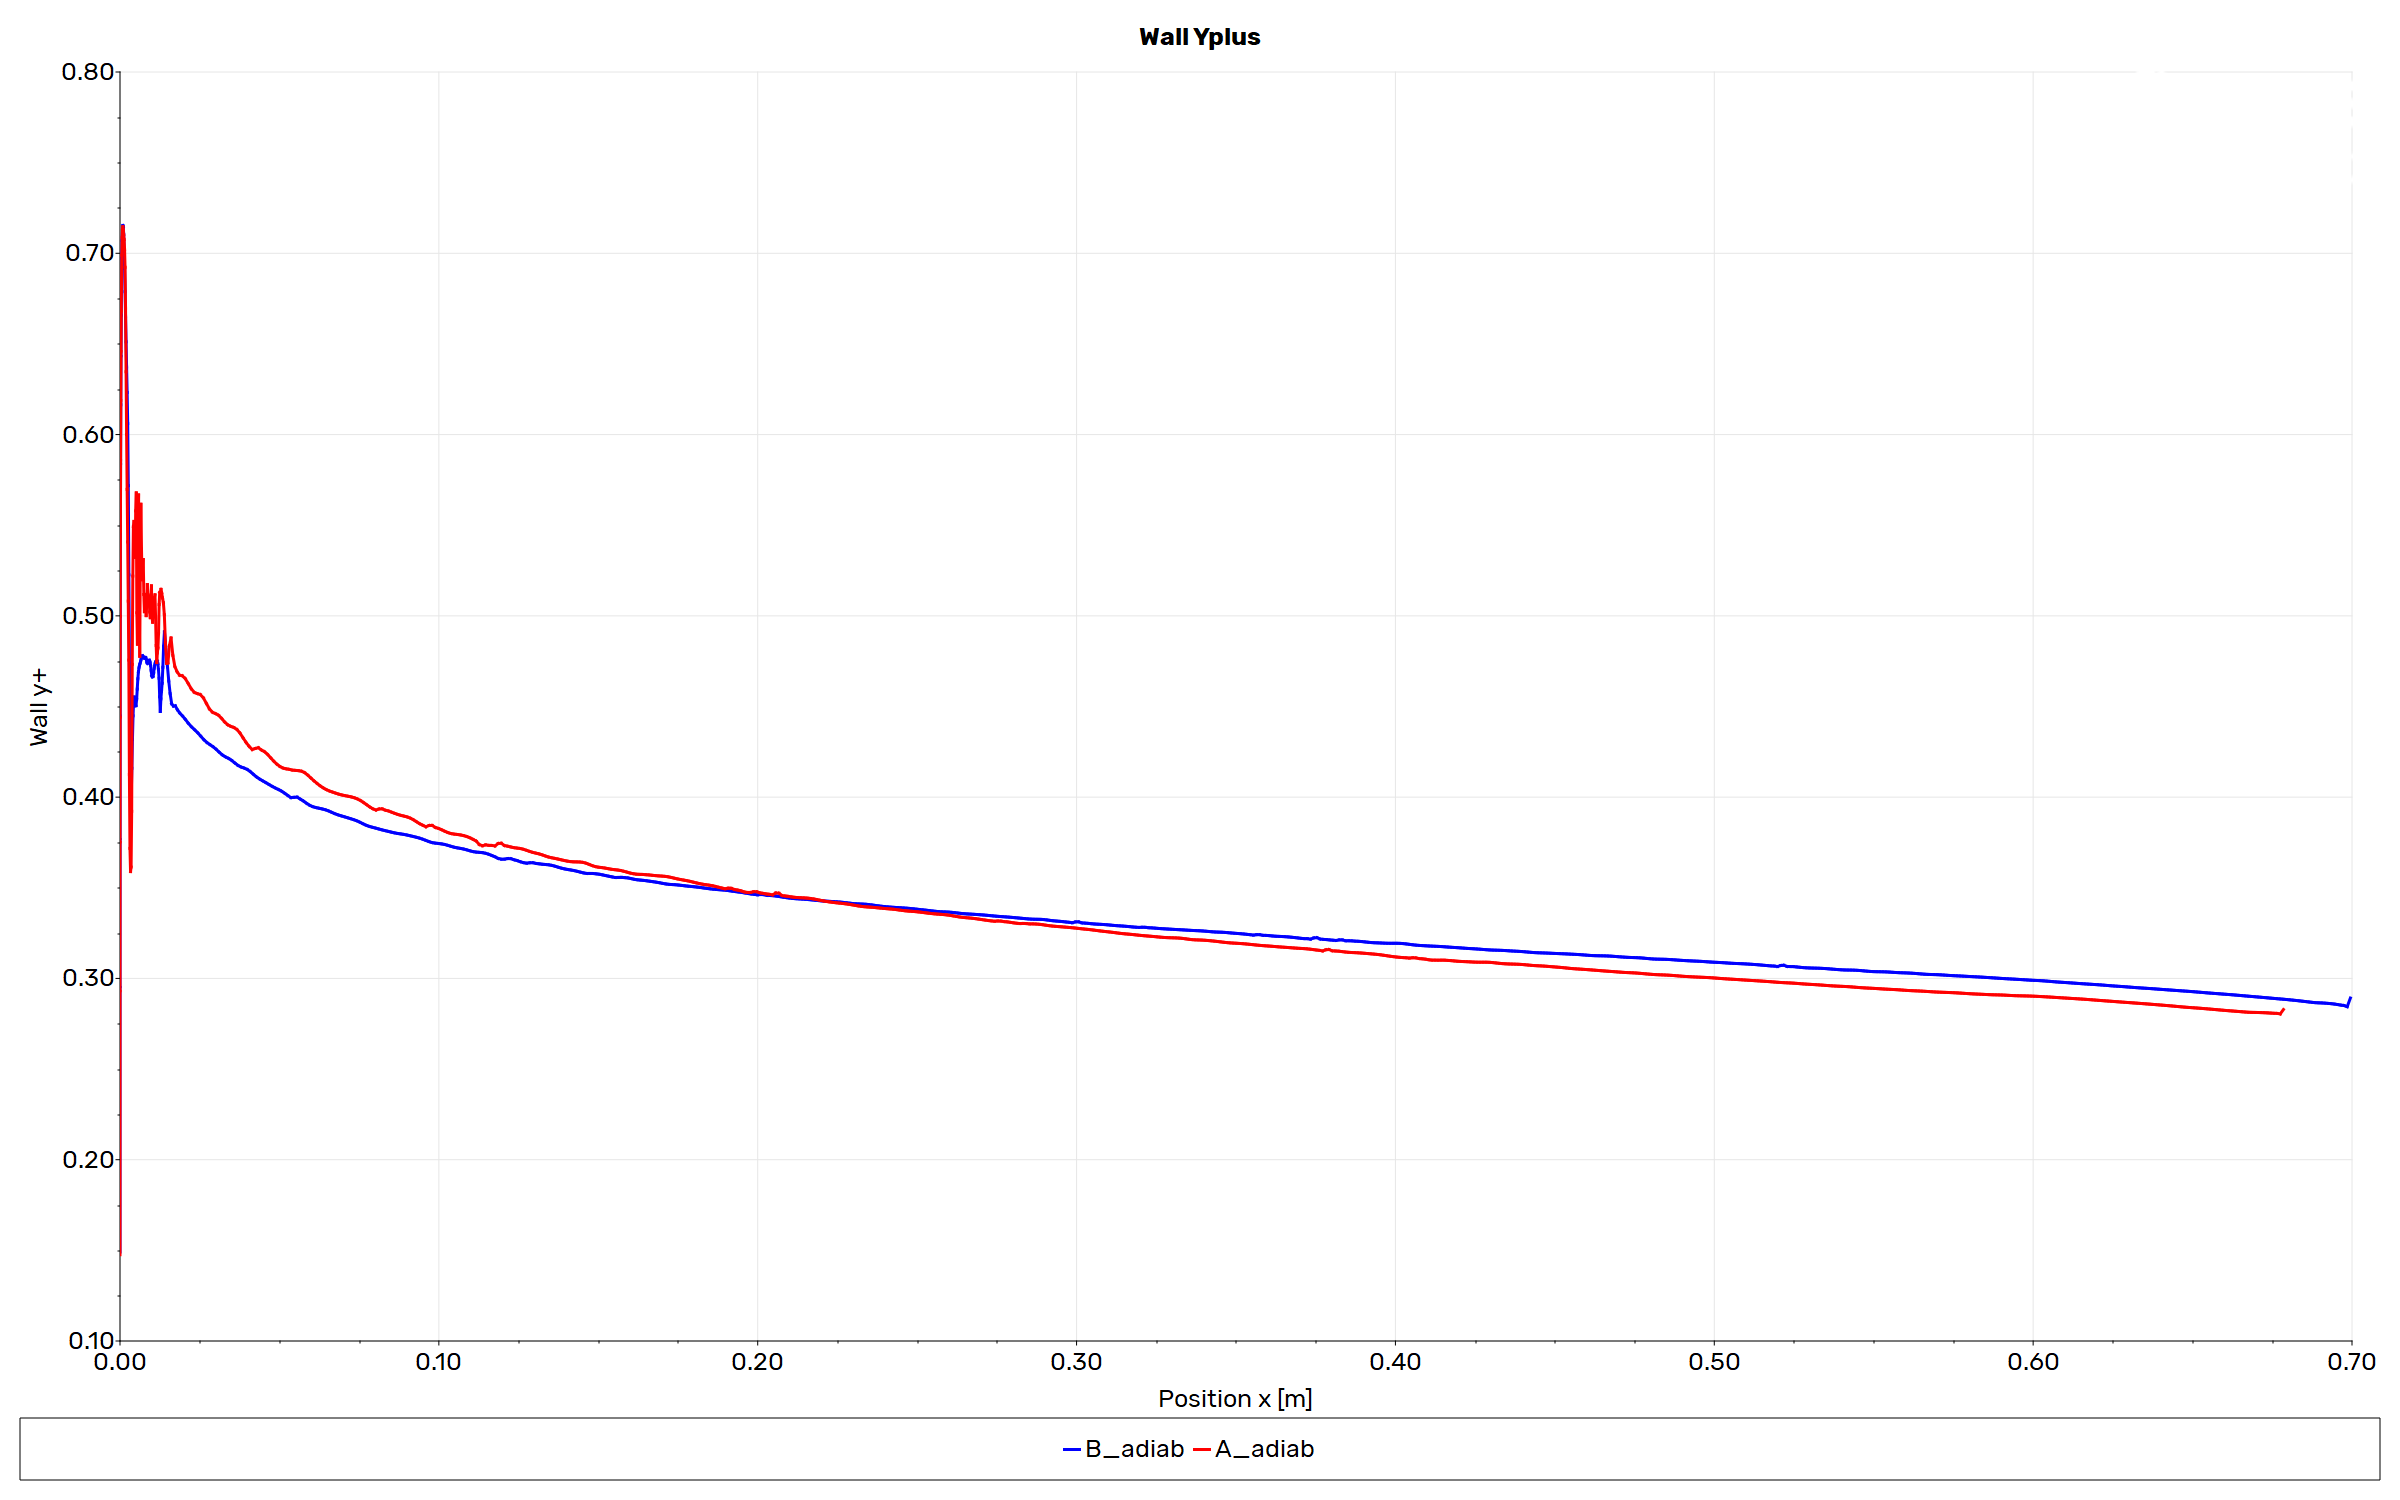
\includegraphics[width=\linewidth]{fluent_yplus_AB_adiab}
\caption{$y^+$ of the first cell along the wall at burnout, design A (red) and B (blue), Fluent.}
\label{fig:yplus}
\end{figure}


\end{document}
